\pagebreak

\chapter{Libraries}\label{ch:libraries}

    \index{library}
    3PL libraries are source files containing modules, procedures,
    functions and global structs and variables which can be accessed by
    application code and other libraries. They are inserted in the
    application source code via a {\bf module} statement or a {\bf source}
    statement (see "file inclusion" \autorefph{sec:fileinclusion}). These
    library files are searched for by the 3PL compiler in the order -
    \blist
    \item   current directory
    \item   directories listed in -I options to the 3PL command line
    \item   directories listed in environment variable {\bf THREEPL\_INCLUDE\_DIRS}
    \blend
    
    3PL libraries may be -
    \blist
    \item   generic
    \item   interfaces to hardware specific to FPGA families
    \item   platform-specific
    \blend
    
    Our libraries are arranged in the following directory structure -
    \begin{verbatim}
        boards/
            avnet/
                aes_sp3a_eval400.3pl
                microzed_7010.3pl
                microzed_7020.3pl
            dangerous_prototypes
                breakout_xc2c64a.3pl
                breakout_xc9572xl.3pl
            digilent
                zybo.3pl
            gadgetfactory
                papilio_one_100.3pl
                papilio_one_250.3pl
                papilio_one_500.3pl
                papilio_pro.3pl
            memec/
                v4fx12lc.3pl
                v4fx12mm.3pl
            xilinx/
                ml505.3pl
        capture.3pl
        ctypes.3pl
        divlib.3pl
        DS2431.3pl
        float.3pl
        jsontype.3pl
        multlib.3pl
        qdr2_ram.3pl
        spi.3pl
        stdlib.3pl
        uart.3pl
        uarts.3pl
        xilinx/
            clocks.3pl
            common.3pl
            cpu.3pl
            dsp48.3pl
            gtp_dual.3pl
            io.3pl
            mgt.3pl
            postprocess.3pl
            ppc405lib.3pl
            ppclib.3pl
            ps7.3pl
            uart_cpu.3pl
            xc2s.3pl
            xc2v.3pl
            xc2vp.3pl
            xc3s.3pl
            xc4v.3pl
            xc5v.3pl
            xc6s.3pl
            xc6v.3pl
            xc7.3pl
            xcv.3pl
            zynq_axi.3pl
        zbt_ram.3pl
    \end{verbatim}
    
    The following are generic libraries -
    \blist
    \item   capture.3pl - capture a data stream
    \item   ctypes.3pl - generate C types from 3PL structs and enums
    \item   divlib.3pl - pipelined integer divider
    \item   float.3pl - pipelined floating point modules
    \item   jsontype.3pl - conversion of a 3PL type to a JSON string
    \item   multlib.3pl - pipelined integer multiplier
    \item   qdr2\_ram.3pl - external quad data rate synchronous static RAM interface
    \item   stdlib.3pl - useful elements such as pulse generators, pulse
            stretchers, adder/subtractors, incrementer/decrementers.
    \item   uart.3pl - generalised UART modules
    \item   uarts.3pl - simple UART modules
    \item   spi.3pl - SPI interface
    \item   zbt\_ram.3pl - external zero bus turnaround synchronous static RAM interface
    \blend
    
    DS2431.3pl provides a module to read and write the DS2431 single wire
    EPROM chip.
    
    The libraries in directory {\bf xilinx} contain elements specific to
    FPGA families. The same elements may be contained in several libraries
    with perhaps detail differences in implementation. These libraries are -
    \blist
    \item   clocks.3pl - clock managers and clock buffers
    \item   common.3pl - low-level elements and functions common to all FPGA
            families
    \item   cpu.3pl - interface between the FPGA and a CPU
    \item   dsp48.3pl - Virtex4 and later DSP blocks
    \item   gtp\_dual.3pl - a GTP dual multi-gigabit transceiver tile
    \item   io.3pl - input/output functions for Virtex5 and later
    \item   mgt.3pl - an MGT transceiver
    \item   postprocess.3pl - a module to generate the configuration file from
            the EDIF file using ISE or VIVADO
    \item   ppc405lib.3pl - an embedded PowerPC instance with instruction and data RAMs
    \item   ppclib.3pl - interface for an embedded PowerPC
    \item   uart\_cpu.3pl - low level UART CPU interface 
    \item   xc2s.3pl - Spartan 2 elements
    \item   xc3s.3pl - Spartan 3 elements
    \item   xc6s.3pl - Spartan 6 elements
    \item   xcv.3pl - Virtex and Virtex-E elements
    \item   xc2v.3pl - Virtex2 elements
    \item   xc2vp.3pl - Virtex2Pro elements
    \item   xc4v.3pl - Virtex 4 elements
    \item   xc5v.3pl - Virtex 5 elements
    \item   xc6v.3pl - Virtex 6 elements
    \item   xc7.3pl - Artix 7, Kintex 7, Virtex 7 and Zynq 7000 elements
    \item   zynq\_axi.3pl - Zynq PL instance and AXI interface to CPU
    \blend

    Directory {\bf boards} contains header files for a variety of FPGA
    boards. Some of these are (or were) commercially available and the
    others were developed in-house by our CSIRO group or by our collaborators.
    These non-commercial boards are included for two reasons - firstly
    we use this documentation ourselves for reference and secondly these files
    illustrate 3PL coding techniques that will be applicable to other FPGA
    platforms.
    
    The {\bf boards} directory contains header files for commercial
    Xilinx boards. There are four subdirectories, avnet, xilinx, memec and
    gadgetfactory.
    
    The {\bf avnet} directory contains header files for Xilinx boards supplied
    by AVNET. At the moment there are four -
    \blist
    \item   aes\_sp3a\_eval400.3pl - Avnet Xilinx Spartan3A evaluation kit
    \item   microzed\_7010.3pl - Avnet Xilinx xc7010 microzed Zynq evaluation kit
    \item   microzed\_7020.3pl - Avnet Xilinx xc7020 microzed Zynq evaluation kit
    \blend

    The {\bf digilent} directory contains one header file for the Digilent zybo
    Zynq evaluation board.
    \blist
    \item   zybo.3pl - Digilent Zybo Zynq evaluation kit
    \blend
    
    The {\bf xilinx} directory contains header files for Xilinx boards supplied
    from Xilinx. At the moment there is one -
    \blist
    \item   ml505.3pl - Xilinx Virtex-5 evaluation board
    \blend
    This file does not support all features of the board.
    
    The {\bf memec} directory contains header files for Xilinx boards supplied
    from Memec. At the moment there are two -
    
    \blist
    \item   v4fx12lc.3pl - Xilinx Virtex4 demonstration board
    \item   v4fx12mm.3pl - Xilinx Virtex4 mini module board
    \blend
    These files so far are only the equivalent of "hello world" and provide
    only the main clock, an optional divided clock and a few pin definitions.

    The {\bf gadgetfactory} directory contains header files for papilio boards
    supplied by the Gadget Factory. At the moment there are four -
    
    \blist
    \item   papilio\_one\_100.3pl - Papilio board with XC3S100E Spartan 3E
    \item   papilio\_one\_250.3pl - Papilio board with XC3S250E Spartan 3E
    \item   papilio\_one\_500.3pl - Papilio board with Xc3S500E Spartan 3E
    \item   papilio\_pro.3pl - Papilio board with XC6SLX9 Spartan
    \blend

    Note that these library files are often also refered to as "header" files
    since they define FPGA pinouts and establish clocks as well as defining
    modules, procedures and functions.

    For an embedded Virtex2 PRO FPGA the program must begin as
    follows -
    \begin{lstlisting}[gobble=8, language=threepl]
       part("XC2VP4FG456-6");      // for example Virtex2 Pro               
    \end{lstlisting}
    but this is usually inclyded in the header file for the device, e.g.
    \begin{lstlisting}[gobble=8, language=threepl]
       module "xilinx/xc2vp.3pl"   // Virtex2 PRO 3PL library
    \end{lstlisting}
    There are matching files for each platform, e.g. xc2s.3pl, xc3s.3pl,
    xcv.3pl, xc7a.3pl etc. It is then useful to inlude the libraries -
    \begin{lstlisting}[gobble=8, language=threepl]
       module "xilinx/common.3pl"  // common Xilinx 3PL library
       module "stdlib.3pl"         // standard 3PL library
    \end{lstlisting}
    Other libraries to be included may be - \\
    xilinx/mgt.3pl\\
    xilinx/gtp\_dual.3pl\\
    xilinx/ppclib.3pl\\
    ctypes.3pl\\
    mutex.3pl\\
    and others.

    The program must include code for establishing clocks and applying
    timing constraints appropriate to those clocks.
    
    
\pagebreak

\heading{Platform-specific module files}

    There is a module file for each Xilinx platform device that should
    be included in source code.

    These files must be incorporated by using a {\bf module} statement,
    e.g. -
    \begin{lstlisting}[gobble=4, language=threepl]
       module "xilinx/xc2s.3pl"
    \end{lstlisting}
    
    Each of these module files includes other module files appropriate
    to the platform device. This avoids the necessity to include these
    files in the source code.
    
    Note that libraries exist for MGT and GTP serial channels, but not yet
    for GTX, GTH or GTZ. Also the GT11 element for Virtex4 has not been
    implemented.

    \begin{tabular}{| l | l | l |}
    \hline
    module file      & device                          & includes module files  \\
    \hline \hline
    xilinx/xc2s.3pl  & Spartan2                        & stdlib.3pl \\
                     &                                 & xilinx/common.3pl \\
                     &                                 & xilinx/clocks.3pl \\ \hline
    xilinx/xc3s.3p   & Spartan3                        & stdlib.3pll \\
                     &                                 & xilinx/common.3pl \\
                     &                                 & xilinx/clocks.3pl \\ \hline
    xilinx/xc6s.3pl  & Spartan6                        & stdlib.3pl \\
                     &                                 & xilinx/common.3pl \\
                     &                                 & xilinx/clocks.3pl \\
                     &                                 & xilinx/io.3pl \\ \hline
    xilinx/xcv.3p    & Virtex and Virtex-E             & stdlib.3pl \\
                     &                                 & xilinx/common.3pl \\
                     &                                 & xilinx/clocks.3pl \\ \hline
    xilinx/xcv2.3pl  & Virtex2                         & stdlib.3pll \\
                     &                                 & xilinx/common.3pl \\
                     &                                 & xilinx/clocks.3pl \\ \hline
    xilinx/xcv2p.3pl & Virtex2 Pro                     & stdlib.3pl \\
                     &                                 & xilinx/common.3pl \\
                     &                                 & xilinx/clocks.3pl \\
                     &                                 & xilinx/ppclib.3pl \\
                     &                                 & xilinx/mgt.3pl \\ \hline
    xilinx/xcv4.3pl  & Virtex4                         & stdlib.3pl \\
                     &                                 & xilinx/common.3pl \\
                     &                                 & xilinx/clocks.3pl \\
                     &                                 & xilinx/io.3pl \\
                     &                                 & xilinx/dsp48.3pl \\
                     &                                 & xilinx/ppclib.3pl \\ \hline
    xilinx/xcv5.3pl  & Virtex5                         & stdlib.3pl \\
                     &                                 & xilinx/common.3pl \\
                     &                                 & xilinx/clocks.3pl \\
                     &                                 & xilinx/io.3pl \\
                     &                                 & xilinx/dsp48.3pl \\
                     &                                 & xilinx/ppclib.3pl \\
                     &                                 & xilinx/gtp\_dual.3pl \\ \hline
    xilinx/xcv6.3pl  & Virtex6                         & stdlib.3pl \\
                     &                                 & xilinx/common.3pl \\
                     &                                 & xilinx/clocks.3pl \\
                     &                                 & xilinx/io.3pl \\
                     &                                 & xilinx/dsp48.3pl \\
                     &                                 & xilinx/ppclib.3pl \\
                     &                                 & xilinx/gtp\_dual.3pl \\ \hline
    xilinx/xc7.3pl   & Artix7 Kintex7 Virtex7 Zynq7000 & stdlib.3pl \\
                     &                                 & xilinx/common.3pl \\
                     &                                 & xilinx/clocks.3pl \\
                     &                                 & xilinx/io.3pl \\
                     &                                 & xilinx/dsp48.3pl \\
                     &                                 & xilinx/gtp\_dual.3pl \\ \hline
    xilinx/zynq\_axi.3pl & Zynq7000 & \\ \hline
    
    \end{tabular}
    



\pagebreak

\section{Clock Manager and Clock Buffer Library File - xilinx/clocks.3pl}

    \index{library!xilinx/clocks.3pl}
    This library creates any clock managers or clock buffers for all Xilinx
    FPGAs.
    
    This library must be incorporated by using a {\bf module} statement -
    \begin{lstlisting}[gobble=4, language=threepl]
       module "xilinx/clocks.3pl"
    \end{lstlisting}
    
    {\bf This library is already incorporated by all FPGA family header files.}
    
    The procedures in this library attempt to propagate clock frequencies and
    periods from inputs to outputs using the parameters controlling clock
    division or synthesis. For that reason most take an error exit if an input
    clock does not have a frequency-period attribute.

    At the moment clkmmcm(), pll\_adv() are exceptions to the last paragraph.
    They will be changed to conform ASAP.
    
    Where clock input pads, clock buffers and clock manager are interconnected
    clock mode variables are used (required by parameter modes). Where a clock
    is derived from CLB logic the inbuilt function {\bf clockfromexpr()}
    \autorefph{sec:ipclockfromexpr} can be used to assign a value mode variable
    to a clock mode variable. Where input delays are required for an input clock
    path (see {\bf idelay()} \autorefph{sec:lpidelay}) the input should be input
    mode rather than clock mode. The output from the delay can then be convert
    to clock mode by using {\bf clockfromexpr()}.



    \subsection{library modules}
    
        None.


    \subsection{library procedures}

        \subsubsection{clkdcm - create a Spartan3, Virtex2, Virtex2Pro, Virtex4 or Virtex5 DCM digital clock manager}\label{sec:lpclkdcm}
            
            {\bf Library: xilinx/clocks.3pl}

            {\bf Prototype:} \\
            \vsp
            \begin{lstlisting}[gobble=12, language=threepl]
               global procedure
               clkdcm (
                   clock({clk0, clk90, clk180, clk270, clk2x, clk2x180, clkdv, clkfx, clkfx180}),
                   value({locked, psdone, drdy}, "log"), value(dout, "uint:16"), value(status, "uint:8")
                   <-
                   str(loc), log({clkin_divide_by_2, duty_cycle_correction, startup_wait}),
                   str(clkdv_divide),
                   float(clkin_period), int({clkfx_divide, clkfx_multiply, phase_shift}),
                   str({clk_feedback,
                   clkout_phase_shift, dfs_frequency_mode, dll_frequency_mode, deskew_adjust}),
                   clock({clkin, clkfb, psclk}), value({reset, psincdec, psen, dwe, den}, "log"),
                   value(din, "bits:16"), value(daddr, "uint:7")
               ) {}
            \end{lstlisting}

            {\bf Output parameters:} \\
            \begin{tabular}{| l | l | l | l |}
            \hline
                           & mode  & type   & \\
            \hline \hline
            {\bf clk0}     & clock &         & output clock \\ \hline
            {\bf clk90}    & clock &         & output clock shifted 90$\deg$ \\ \hline
            {\bf clk180}   & clock &         & output clock shifted 180$\deg$ \\ \hline
            {\bf clk270}   & clock &         & output clock shifted 270$\deg$ \\ \hline
            {\bf clk2x}    & clock &         & output clock at double frequency \\ \hline
            {\bf clk2x180} & clock &         & output clock at double frequency shifted 180$\deg$ \\ \hline
            {\bf clkdv}    & clock &         & divided output clock \\ \hline
            {\bf clkfx}    & clock &         & frequency synthesised output clock \\ \hline
            {\bf clkfx180} & clock &         & frequency synthesised output clock shifted 180$\deg$ \\ \hline
            {\bf locked}   & value & log     & DLL is locked \\ \hline
            {\bf status}   & value & uint:8  & status \\ \hline
            {\bf psdone}   & value & log     & phase shift has finished \\ \hline
            {\bf drdy}     & value & log     & DCM ready for reconfiguration \\ \hline
            {\bf dout}     & value & bits:16 & status and reconfiguration data output \\ \hline
            \end{tabular}

            {\bf Input parameters:} \\            
            \begin{tabular}{| l | l | l | l |}
            \hline
                           & mode  & type   & \\
            \hline \hline
            {\bf loc}                     & immediate & str   & optional location \\ \hline
            {\bf clkin\_divide\_by\_2}    & immed     & log   & DLL clock output at $f_{in}/2$ \\ \hline
            {\bf duty\_cycle\_correction} & immediate & log   & correct duty cycle to 50\%  \\ \hline
            {\bf startup\_wait}           & immediate & log   & delay startup on lock \\ \hline
            {\bf clkdv\_divide}           & immed     & str   & $n$ for clock output at $f_{in}/n$ \\ \hline
            {\bf clkin\_period}           & immediate & float & input clock period, ns \\ \hline
            {\bf clkfx\_divide}           & immed     & int   & $m$ for DFS clock output at $f_{in} \times n / m$ \\ \hline
            {\bf clkfx\_multiply}         & immed     & int   & $n$ for DFS clock output at $f_{in} \times n / m$ \\ \hline
            {\bf phase\_shift}            & immediate & int   & fixed phase shift value \\ \hline
            {\bf clk\_feedback}           & immediate & str   & "1x", "2x", "none" \\ \hline
            {\bf clkout\_phase\_shift}    & immediate & str   & "none", "fixed", "variable" \\ \hline
            {\bf dfs\_frequency\_mode}    & immediate & str   & "high" or "low" \\ \hline
            {\bf dll\_frequency\_mode}    & immediate & str   & "high" or "low" \\ \hline
            {\bf deskew\_adjust}          & immediate & str   & "system\_synchronous", "source\_synchronous", or 0 - 15 \\ \hline
            {\bf clkin}                   & clock     &       & input clock \\ \hline
            {\bf clkfb}                   & clock     &       & clock feedback \\ \hline
            {\bf psclk}                   & clock     &       & phase shift clock\\ \hline
            {\bf reset}                   & value     & log   & reset \\ \hline
            {\bf psincdec}                & value     & log   & phase shift increment or decrement\\ \hline
            {\bf psen}                    & value     & log   & phase shift enable\\ \hline
            {\bf dwe}                     & value     & log   & reconfiguration data write enable\\ \hline
            {\bf den}                     & value     & log   & select reconfiguration data or status output\\ \hline
            {\bf din}                     & value     & log   & reconfiguration data input \\
            {\bf daddr}                   & value     & log   & reconfiguration address input \\ \hline
            \end{tabular}

            {\bf In-line target execution:} \\
            no

            {\bf description:} \\
            Creates a Virtex4 or Virtex5 DCM digital clock manager. See Xilinx
            documentation for signal and attribute details. The first group of input
            parameters are immediate mode and are attributes. The remaining input
            parameters are input signals, clock mode for clocks and value mode for
            control signals.

            \heading{Attributes}

                {\bf loc} is an optional location string from the
                following list - "DLL0P", "DLL1P", "DLL2P", "DLL3P", "DLL0S", "DLL1S",
                "DLL2S", "DLL3S". These select from the four primary and four secondary
                delay-locked loops. If "" it is ignored.

                {\bf clkin\_divide\_by\_2} - see Xilinx documentation.

                If {\bf duty\_cycle\_correction} is true or missing then duty cycle
                correction is enabled, giving a DLL output duty cycle of 50\%. If
                this attribute is false then the duty cycle will be the same as that
                of the input.

                {\bf startup\_wait} if true causes startup following configuration to
                be delayed until the DCM achieves lock.

                {\bf clkfx\_divide} is the frequency divider for the DFS (1 to 32).

                {\bf clkfx\_multiply} is the frequency multiplier for the DFS (2 to 32).


                {\bf phase\_shift} is the phase shift value which must be in the
                range -255 to +255 inclusive. A unit value represents 1/256 of a cycle.

                {\bf clkdv\_divide} indicates that the divided
                frequency output is being used. The division ratio is a
                string argument which must be one of "1.5", "2.0", "2.5", "3.0",
                "3.5", "4.0", "4.5", "5.0", "5.5", "6.0", "6.5", "7.0", "7.5", "8.0",
                "9.0", "10.0", "11.0", "12.0", "13.0", "14.0", "15.0" or "16.0".

                {\bf clkin\_period} is the input clock period. This must be
                specified if the DFS is used.

                {\bf clk\_feedback} must be "2X" if the clock feedback is at twice
                input frequency. By default the feedback is at the input frequency, or
                this attribute can be explcitly "1X" to achieve the same.

                {\bf clkout\_phase\_shift} is a string selecting the mode of the
                phase shifter. If omitted or "none" the outputs are not phase shifted.
                If this argument is "fixed" a clock skew is added to the input clock
                shifting the phase of all clock outputs. The phase shift is specified by
                the next input argument. If "variable" is specified the phase shift
                is initially set as specified by the next argument, but it can be
                dynamically incremented or decremented - see the 17th to 19th input
                arguments. On reset the phase shift returns to the initial value.

                {\bf dfs\_frequency\_mode} indicates that the DFS is on
                the high frequency range. The low and high frequency ranges are
                given in the data sheets.

                {\bf dll\_frequency\_mode} indicates that the DLL is in
                the high frequency range (see data sheets). In this mode the 90 degree
                and 270 degree outputs and the 2X frequency outputs  are not available.

                {\bf deskew\_adjust} controls the amount of delay in the feedback
                path. Its values can be "system\_synchronous" (default),
                "source\_synchronous" or "0 to 15".

                {\bf dcm\_performance\_mode} optimises the DCM for high frequency low jitter
                ("max\_speed", the default) or low frequency and maximum phase shift range
                ("max\_range").

            \heading{input signals}
            
                {\bf din}, {\bf daddr}, {\bf dwe},  {\bf den} and {\bf dclk}
                are only available on Virtex4 and Virtex5.

                {\bf clkin} is the input clock. This argument must be
                supplied and is the first target mode input argument.

                {\bf clkfb} is the clock feedback. This argument must be
                supplied. This is usually a buffered version of the output clock at
                phase 0.

                {\bf reset} is an optional reset. This resets the
                DLL, DFS and phase shifter and re-establishes lock.

                {\bf psincdec} is true if a phase increment is to be
                executed or false if a phase decrement is to be executed. Execution is
                controlled by the following two inputs.

                {\bf psen} is the phase increment/decrement enable.
                This must be held true for one period of the phase shift adjustment
                clock (the next input argument). 

                {\bf psclk} is the phase increment/decrement clock.

                {\bf din} is data input for a dynamic reconfiguration write.

                {\bf daddr} is the address input for a dynamic reconfiguration
                write.

                {\bf dwe} is driven high for one {\bf dclk} cycle along with
                {\bf den} to execute a dynamic reconfiguration write.

                {\bf den} is driven high for one {\bf dclk} cycle to execute
                a dynamic reconfiguration read or write.

                {\bf dclk} is a clock controlling dynamic reconfiguration
                operations.

            \heading{output signals}

                {\bf drdy} and {\bf dout} are only available on Virtex4 and
                Virtex5.
                
                {\bf status} is only available on Spartan3, Virtex2 and Virtex2Pro.
                
                {\bf clk0}, {\bf clk90}, {\bf clk180} and {\bf clk270} are clock
                outputs at the input frequency. These are at phases 0, 90, 180 and 270
                degree respectively relative to the input clock.

                {\bf clk2x} and {\bf clk2x180} are at twice the input frequency
                at phases 0 and 180 degree respectively.

                {\bf clkdv} is the divided clock frequency where the division ratio
                is given by the 3rd input argument.

                {\bf clkfx} and {\bf clkfx180} are the frequency synthesised clock
                at phases 0 and 180 degree respectively. The frequency is the input
                multiplied by the value of {\bf clkfx\_multiply} and divided by the value
                of {\bf clkfx\_divide}.

                {\bf locked} is high when the DLL and DFS are locked to the input
                clock. This signal has a null clock domain.

                {\bf status} is an 8 bit status (see Xilinx unified library
                documentation). This signal has a null clock domain.

                {\bf psdone} goes high when a phase shift adjustment has been done.
                It remains high for one period of the phase adjustment clock. Note
                that this signal has a null clock domain, but it is synchronous
                with {\bf psclk}.

                {\bf drdy} goes high when the dynamic configuration port finishes
                an operation. On a read the data on {\bf do} must be captured on
                the next rising {\bf dclk} edge. When writing the next operation
                can commence on the same clock cycle in which {\bf drdy} goes high.

                {\bf dout} is the data output when reading dynamic configuration data.
                The data on {\bf do} must be captured on
                the rising {\bf dclk} edge when {\bf drdy} is high.



        \subsubsection{clkdll - create a Spartan2, Virtex or VirtexE DLL delay-locked loop clock manager}\label{sec:lpclkdll}
            
            {\bf Library: xilinx/clocks.3pl}

            {\bf Prototype:} \\
            \vsp
            \begin{lstlisting}[gobble=12, language=threepl]
               global procedure
               clkdlle (
                   clock({clk0, clk90, clk180, clk270, clk2x, clkdv}),
                   value(locked, "log")
                   <-
                   str(loc), log({duty_cycle_correction, startup_wait}),
                   int(clkdv_divide),
                   clock({clkin, clkfb}), value(reset, "log")
               ) {}
            \end{lstlisting}

            {\bf Output parameters:} \\
            \begin{tabular}{| l | l | l | l |}
            \hline
                           & mode  & type   & \\
            \hline \hline
            {\bf clk0}     & clock &        & output clock \\ \hline
            {\bf clk90}    & clock &        & output clock shifted 90$\deg$ \\ \hline
            {\bf clk180}   & clock &        & output clock shifted 180$\deg$ \\ \hline
            {\bf clk270}   & clock &        & output clock shifted 270$\deg$ \\ \hline
            {\bf clk2x}    & clock &        & output clock at double frequency \\ \hline
            {\bf clkdv}    & clock &        & divided output clock \\ \hline
            \end{tabular}

            {\bf Input parameters:} \\            
            \begin{tabular}{| l | l | l | l |}
            \hline
                           & mode  & type   & \\
            \hline \hline
            {\bf loc}                     & immediate & str   & optional location \\ \hline
            {\bf clkin\_divide\_by\_2}    & immediate & log   & divide clock by 2 \\ \hline
            {\bf duty\_cycle\_correction} & immediate & log   & correct duty cycle \\ \hline
            {\bf startup\_wait}           & immediate & log   & delay startup on lock \\ \hline
            {\bf clkdv\_divide}           & immediate & int   & clock division ratio \\ \hline
            {\bf clkin}                   & clock     &       & input clock \\ \hline
            {\bf clkfb}                   & clock     &       & clock feedback \\ \hline
            {\bf reset}                   & value     & log   & reset \\ \hline
            \end{tabular}

            {\bf In-line target execution:} \\
            no

            {\bf description:} \\
            Creates a Virtex DLL delay-locked loop clock manager. See Xilinx
            documentation for signal and attribute details. The first group of input
            parameters are immediate mode and are attributes. The remaining input
            parameters are input signals, clock mode for clocks and value mode for
            control signals.

            \heading{attributes}

                {\bf loc} is an optional location string from the
                following list - "DLL0P", "DLL1P", "DLL2P", "DLL3P", "DLL0S", "DLL1S",
                "DLL2S", "DLL3S". These select from the four primary and four secondary
                delay-locked loops. If "" it is ignored.

                {\bf clkin\_divide\_by\_2} - see Xilinx documentation.

                If {\bf duty\_cycle\_correction} is true or missing then duty cycle
                correction is enabled, giving a DLL output duty cycle of 50\%. If
                this attribute is false then the duty cycle will be the same as that
                of the input.

                {\bf startup\_wait} if true causes startup following configuration to
                be delayed until the DLL achieves lock.

                {\bf clkdv\_divide} indicates that the divided
                frequency output is being used. The division ratio is a
                string argument which must be an integer from 1 to 32 inclusive.

            \heading{input signals}

                {\bf clkin} is the input clock. This argument must be
                supplied and is the first target mode input argument.

                {\bf clkfb} is the clock feedback. This argument must be
                supplied. This is usually a buffered version of the output clock at
                phase 0.

                {\bf reset} is an optional reset. This resets the
                DLL, DFS and phase shifter and re-establishes lock.
                operations.

            \heading{output signals}

                {\bf clk0}, {\bf clk90}, {\bf clk180} and {\bf clk270} are clock
                outputs at the input frequency. These are at phases 0, 90, 180 and 270
                degree respectively relative to the input clock.

                {\bf clk2x} is at twice the input frequency.

                {\bf clkdv} is the divided clock frequency where the division ratio
                is given by the 3rd input argument.

                {\bf locked} is high when the DLL and DFS are locked to the input
                clock. This signal has a null clock domain.






        \subsubsection{clkdlle - create an extended Spartan2, Virtex or VirtexE DLL delay-locked loop clock manager}\label{sec:lpclkdlle}
            
            {\bf Library: xilinx/clocks.3pl}

            {\bf Prototype:} \\
            \vsp
            \begin{lstlisting}[gobble=12, language=threepl]
               global procedure
               clkdlle (
                   clock({clk0, clk90, clk180, clk270, clk2x, clk2x180, clkdv}),
                   value(locked, "log")
                   <-
                   str(loc), log({duty_cycle_correction, startup_wait}),
                   int(clkdv_divide),
                   clock({clkin, clkfb}), value(reset, "log")
               ) {}
            \end{lstlisting}

            {\bf Output parameters:} \\
            \begin{tabular}{| l | l | l | l |}
            \hline
                           & mode  & type   & \\
            \hline \hline
            {\bf clk0}     & clock &        & output clock \\ \hline
            {\bf clk90}    & clock &        & output clock shifted 90$\deg$ \\ \hline
            {\bf clk180}   & clock &        & output clock shifted 180$\deg$ \\ \hline
            {\bf clk270}   & clock &        & output clock shifted 270$\deg$ \\ \hline
            {\bf clk2x}    & clock &        & output clock at double frequency \\ \hline
            {\bf clk2x180} & clock &        & output clock at double frequency shifted 180$\deg$ \\ \hline
            {\bf clkdv}    & clock &        & divided output clock \\ \hline
            \end{tabular}

            {\bf Input parameters:} \\            
            \begin{tabular}{| l | l | l | l |}
            \hline
                           & mode  & type   & \\
            \hline \hline
            {\bf loc}                     & immediate & str   & optional location \\ \hline
            {\bf clkin\_divide\_by\_2}    & immediate & log   & divide clock by 2 \\ \hline
            {\bf duty\_cycle\_correction} & immediate & log   & correct duty cycle \\ \hline
            {\bf startup\_wait}           & immediate & log   & delay startup on lock \\ \hline
            {\bf clkdv\_divide}           & immediate & int   & clock division ratio \\ \hline
            {\bf clkin}                   & clock     &       & input clock \\ \hline
            {\bf clkfb}                   & clock     &       & clock feedback \\ \hline
            {\bf reset}                   & value     & log   & reset \\ \hline
            \end{tabular}

            {\bf In-line target execution:} \\
            no

            {\bf description:} \\
            Creates a Virtex DLLE extended delay-locked loop clock manager. See
            Xilinx documentation for signal and attribute details. The first group
            of input parameters are immediate mode and are attributes. The remaining
            input parameters are input signals, clock mode for clocks and value mode
            for control signals.

            \heading{attributes}

                {\bf loc} is an optional location string from the
                following list - "DLL0P", "DLL1P", "DLL2P", "DLL3P", "DLL0S", "DLL1S",
                "DLL2S", "DLL3S". These select from the four primary and four secondary
                delay-locked loops. If "" it is ignored.

                {\bf clkin\_divide\_by\_2} - see Xilinx documentation.

                If {\bf duty\_cycle\_correction} is true or missing then duty cycle
                correction is enabled, giving a DLL output duty cycle of 50\%. If
                this attribute is false then the duty cycle will be the same as that
                of the input.

                {\bf startup\_wait} if true causes startup following configuration to
                be delayed until the DLL achieves lock.

                {\bf clkdv\_divide} indicates that the divided
                frequency output is being used. The division ratio is a
                string argument which must be an integer from 1 to 32 inclusive.

            \heading{input signals}

                {\bf clkin} is the input clock. This argument must be
                supplied and is the first target mode input argument.

                {\bf clkfb} is the clock feedback. This argument must be
                supplied. This is usually a buffered version of the output clock at
                phase 0.

                {\bf reset} is an optional reset. This resets the
                DLL, DFS and phase shifter and re-establishes lock.
                operations.

            \heading{output signals}

                {\bf clk0}, {\bf clk90}, {\bf clk180} and {\bf clk270} are clock
                outputs at the input frequency. These are at phases 0, 90, 180 and 270
                degree respectively relative to the input clock.

                {\bf clk2x} and {\bf clk2x180} are at twice the input frequency
                at phases 0 and 180 degree respectively.

                {\bf clkdv} is the divided clock frequency where the division ratio
                is given by the 3rd input argument.

                {\bf locked} is high when the DLL and DFS are locked to the input
                clock. This signal has a null clock domain.






        \subsubsection{clkdllhf - create a high frequency Spartan2, Virtex or VirtexE DLL delay-locked loop clock manager}\label{sec:lpclkdllhf}
            
            {\bf Library: xilinx/clocks.3pl}

            {\bf Prototype:} \\
            \vsp
            \begin{lstlisting}[gobble=12, language=threepl]
               global procedure
               clkdlle (
                   clock({clk0, clk180, clkdv}),
                   value(locked, "log")
                   <-
                   str(loc), log({duty_cycle_correction, startup_wait}),
                   int(clkdv_divide),
                   clock({clkin, clkfb}), value(reset, "log")
               ) {}
            \end{lstlisting}

            {\bf Output parameters:} \\
            \begin{tabular}{| l | l | l | l |}
            \hline
                           & mode  & type   & \\
            \hline \hline
            {\bf clk0}     & clock &        & output clock \\ \hline
            {\bf clk180}   & clock &        & output clock shifted 180$\deg$ \\ \hline
            {\bf clkdv}    & clock &        & divided output clock \\ \hline
            \end{tabular}

            {\bf Input parameters:} \\            
            \begin{tabular}{| l | l | l | l |}
            \hline
                           & mode  & type   & \\
            \hline \hline
            {\bf loc}                     & immediate & str   & optional location \\ \hline
            {\bf clkin\_divide\_by\_2}    & immediate & log   & divide clock by 2 \\ \hline
            {\bf duty\_cycle\_correction} & immediate & log   & correct duty cycle \\ \hline
            {\bf startup\_wait}           & immediate & log   & delay startup on lock \\ \hline
            {\bf clkdv\_divide}           & immediate & int   & clock division ratio \\ \hline
            {\bf clkin}                   & clock     &       & input clock \\ \hline
            {\bf clkfb}                   & clock     &       & clock feedback \\ \hline
            {\bf reset}                   & value     & log   & reset \\ \hline
            \end{tabular}

            {\bf In-line target execution:} \\
            no

            {\bf description:} \\
            Creates a Virtex DLL high frequency delay-locked loop clock manager. See
            Xilinx documentation for signal and attribute details. The first group
            of input parameters are immediate mode and are attributes. The remaining
            input parameters are input signals, clock mode for clocks and value mode
            for control signals.

            \heading{attributes}

                {\bf loc} is an optional location string from the
                following list - "DLL0P", "DLL1P", "DLL2P", "DLL3P", "DLL0S", "DLL1S",
                "DLL2S", "DLL3S". These select from the four primary and four secondary
                delay-locked loops. If "" it is ignored.

                {\bf clkin\_divide\_by\_2} - see Xilinx documentation.

                If {\bf duty\_cycle\_correction} is true or missing then duty cycle
                correction is enabled, giving a DLL output duty cycle of 50\%. If
                this attribute is false then the duty cycle will be the same as that
                of the input.

                {\bf startup\_wait} if true causes startup following configuration to
                be delayed until the DLL achieves lock.

                {\bf clkdv\_divide} indicates that the divided
                frequency output is being used. The division ratio is a
                string argument which must be an integer from 1 to 32 inclusive.

            \heading{input signals}

                {\bf clkin} is the input clock. This argument must be
                supplied and is the first target mode input argument.

                {\bf clkfb} is the clock feedback. This argument must be
                supplied. This is usually a buffered version of the output clock at
                phase 0.

                {\bf reset} is an optional reset. This resets the
                DLL, DFS and phase shifter and re-establishes lock.
                operations.

            \heading{output signals}

                {\bf clk0} and {\bf clk180} are clock
                outputs at the input frequency. These are at phases 0 and 180
                degree respectively relative to the input clock.

                {\bf clkdv} is the divided clock frequency where the division ratio
                is given by the 3rd input argument.

                {\bf locked} is high when the DLL and DFS are locked to the input
                clock. This signal has a null clock domain.






        \subsubsection{simpleclock - create a clock of specified frequency}\label{sec:lpsimpleclock}
            
            {\bf Library: xilinx/clocks.3pl}

            {\bf Prototype:} \\
            \vsp
            \begin{lstlisting}[gobble=12, language=threepl]
               global procedure
               simpleclock (ident(v), clock(in), float(freq), float(tol)) {}
            \end{lstlisting}

            {\bf Output parameters:} \\
            none.

            {\bf Input parameters:} \\            
            \begin{tabular}{| l | l | l | l |}
            \hline
                                          & mode  & type   & \\
            \hline \hline
            {\bf v}     & -         & -       & new clock variable identifier \\ \hline
            {\bf in}    & clock     & -       & input clock                   \\ \hline
            {\bf freq}  & immediate & float   & requested frequency           \\ \hline
            {\bf tol}   & immediate & float   & frequency tolerance           \\ \hline
            \end{tabular}

            {\bf In-line target execution:} \\
            no

            {\bf description:} \\
            Creates a clock variable using a clkdcm and clock buffer as its source.
            {\bf At present it can only be used on FPGA platforms that contain DCMs.}
            
            {\bf v} is an identifier for the new clock mode variable.
            
            {\bf in} is a clock that can be used to drive the DCM.
            
            {\bf freq} is the requested frequency in Hz. If this has no argument
            then the clock frequency will be the same as that of the input clock.
            This can be used to simply add a DCM and clock buffer to an input clock
            from an input buffer.

            {\bf tol} is the allowable tolerance on the requested frequency in Hz.

            If a frequency within the specified tolerance cannot be generated then
            a fatal error occurs.

            This procedure does not attempt to optimise the use of DCMs to generate
            multiple clocks. It uses a new DCM for each call.
            
            The procedure determines the multiplier and divisor which will produce
            the closest synthesiser frequency to that requested. If the requested
            frequency is lower than the input frequency the procedure also attempts
            to find a clock division ratio close to that required to achieve the
            requested frequency. The closest match from the above is then chosen. If
            the resulting frequency is not within tolerance a fatal error occurs.
            
            The clock variable will have the generated frequency attribute, not
            that of the requested frequency.
            
            Example of simple clock input.

            \begin{lstlisting}[gobble=12, language=threepl]
               iopins(c32_pin, "str", "P94", frequency=32.0e6, ibufg=true, iostandard=lvcmos33);

               clock(c32_in, loc=c32_pin);     // clock input from pin and input buffer
               simpleclock(global.c32, c32_in);// global clock
            \end{lstlisting}


            Example of multiple global clocks generated from c32 clock.

            \begin{lstlisting}[gobble=12, language=threepl]
               simpleclock(global.c16, c32, 16.0e6, 0.1);    // 16 MHz clock
               simpleclock(global.c25, c32, 25.0e6, 0.1);    // 25 MHz clock
            \end{lstlisting}




        \subsubsection{clkmmcm\_adv - create an advanced MMCM multi-mode clock manager }\label{sec:lpmmcma}
            
            {\bf Library: xilinx/clocks.3pl}

            {\bf Prototype:} \\
            \vsp
            \begin{lstlisting}[gobble=12, language=threepl]
               global procedure
               clkmmcm_adv (
                   clock({ clkout0, clkout1, clkout2, clkout3, clkout4, clkout5, clkout6,
                           clkout0b, clkout1b, clkout2b, clkout3b, clkfbout, clkfboutb}),
                   value({clkfbstopped, clkinstopped, drdy, locked, psdone}, "log"),
                   value(dout, "bits:16")
                   <-
                   str(loc),

                   log({   clkfbout_use_fine_ps, clkout0_use_fine_ps, clkout1_use_fine_ps,
                           clkout2_use_fine_ps, clkout3_use_fine_ps, clkout4_use_fine_ps,
                           clkout5_use_fine_ps, clkout6_use_fine_ps, clock_hold, startup_wait}),
                   int(divclk_divide),
                   float({ clkfbout_phase, clkfbout_mult_f,
                           clkout0_divide_f,
                           clkout0_duty_cycle, clkout0_phase, clkout1_divide_f,
                           clkout1_duty_cycle, clkout1_phase, clkout2_divide_f,
                           clkout2_duty_cycle, clkout2_phase, clkout3_divide_f,
                           clkout3_duty_cycle, clkout3_phase, clkout4_divide_f,
                           clkout4_duty_cycle, clkout4_phase, clkout5_divide_f,
                           clkout5_duty_cycle, clkout5_phase, clkout6_divide_f,
                           clkout6_duty_cycle, clkout6_phase, ref_jitter1, ref_jitter2}),
                   str(compensation)
                   clock({clkfb, clkin1, clkin2, dclk, psclk}),
                   value({clkinsel, den, dwe, psen, psincdec, pwrdwn, reset}, "log"),
                   value(din, "bits:16"), value(daddr, "uint:7")
               ) {}
            \end{lstlisting}

            {\bf Output parameters:} \\
            \begin{tabular}{| l | l | l | l |}
            \hline
                               & mode  & type   & \\
            \hline \hline
            {\bf clkout0}      & clock &         & output clock 0 \\ \hline
            {\bf clkout1}      & clock &         & output clock 1 \\ \hline
            {\bf clkout2}      & clock &         & output clock 2 \\ \hline
            {\bf clkout3}      & clock &         & output clock 3 \\ \hline
            {\bf clkout4}      & clock &         & output clock 4 \\ \hline
            {\bf clkout5}      & clock &         & output clock 5 \\ \hline
            {\bf clkout6}      & clock &         & output clock 6 \\ \hline
            {\bf clkout0b}     & clock &         & output inverted clock 0 \\ \hline
            {\bf clkout1b}     & clock &         & output inverted clock 1 \\ \hline
            {\bf clkout2b}     & clock &         & output inverted clock 2 \\ \hline
            {\bf clkout3b}     & clock &         & output inverted clock 3 \\ \hline
            {\bf clkfbout}     & clock &         & output clock feedback \\ \hline
            {\bf clkfboutb}    & clock &         & output inverted clock feedback \\ \hline
            {\bf clkfbstopped} & value & log     & clock feedback stopped indicator \\ \hline
            {\bf clkinstopped} & value & log     & input clock stopped indicator \\ \hline
            {\bf drdy}         & value & log     & DRP ready \\ \hline
            {\bf locked}       & value & log     & MMC locked \\ \hline
            {\bf psdone}       & value & log     & phase shift done \\ \hline
            {\bf dout}         & value & log     & DRP data output \\ \hline
            \end{tabular}

            {\bf Input parameters:} \\            
            \begin{tabular}{| l | l | l | l |}
            \hline
                                          & mode  & type   & \\
            \hline \hline
            {\bf loc}                     & immediate & str   & optional location \\ \hline
            {\bf clkfbout\_use\_fine\_ps} & immediate & log   & enable feedback phase shift fine counter \\ \hline
            {\bf clkout0\_use\_fine\_ps}  & immediate & log   & enable output 0 phase shift fine counter  \\ \hline
            {\bf clkout1\_use\_fine\_ps}  & immediate & log   & enable output 1 phase shift fine counter  \\ \hline
            {\bf clkout2\_use\_fine\_ps}  & immediate & log   & enable output 2 phase shift fine counter  \\ \hline
            {\bf clkout3\_use\_fine\_ps}  & immediate & log   & enable output 3 phase shift fine counter  \\ \hline
            {\bf clkout4\_use\_fine\_ps}  & immediate & log   & enable output 4 phase shift fine counter  \\ \hline
            {\bf clkout5\_use\_fine\_ps}  & immediate & log   & enable output 5 phase shift fine counter  \\ \hline
            {\bf clkout6\_use\_fine\_ps}  & immediate & log   & enable output 6 phase shift fine counter  \\ \hline
            {\bf clock\_hold}             & immediate & log   & not documented \\ \hline
            {\bf startup\_wait}           & immediate & log   & delay startup on lock \\ \hline
            {\bf divclk\_divide}          & immediate & int   & divider ratio, 1 to 128 \\ \hline
            {\bf clkfbout\_phase}         & immediate & float & clock feedback phase, -360.0 to 360.0\\ \hline
            {\bf clkfbout\_mult\_f}       & immediate & float & clock feedback multiplier, 1.0 to 64.0\\ \hline
            {\bf clkout0\_divide\_f}      & immediate & float & clock 0 divider, 1.0 to 128.0\\ \hline
            {\bf clkout0\_duty\_cycle}    & immediate & float & clock 0 duty cycle, 0.001 to 0.999\\ \hline
            {\bf clkout0\_phase}          & immediate & float & clock 0 phase, -360.0 to 360.0\\ \hline
            {\bf clkout1\_divide\_f}      & immediate & float & clock 1 divider, 1.0 to 128.0\\ \hline
            {\bf clkout1\_duty\_cycle}    & immediate & float & clock 1 duty cycle, 0.001 to 0.999\\ \hline
            {\bf clkout1\_phase}          & immediate & float & clock 1 phase, -360.0 to 360.0\\ \hline
            {\bf clkout2\_divide\_f}      & immediate & float & clock 2 divider, 1.0 to 128.0\\ \hline
            {\bf clkout2\_duty\_cycle}    & immediate & float & clock 2 duty cycle, 0.001 to 0.999\\ \hline
            {\bf clkout2\_phase}          & immediate & float & clock 2 phase, -360.0 to 360.0\\ \hline
            {\bf clkout3\_divide\_f}      & immediate & float & clock 3 divider, 1.0 to 128.0\\ \hline
            {\bf clkout3\_duty\_cycle}    & immediate & float & clock 3 duty cycle, 0.001 to 0.999\\ \hline
            {\bf clkout3\_phase}          & immediate & float & clock 3 phase, -360.0 to 360.0\\ \hline
            {\bf clkout4\_divide\_f}      & immediate & float & clock 4 divider, 1.0 to 128.0\\ \hline
            {\bf clkout4\_duty\_cycle}    & immediate & float & clock 4 duty cycle, 0.001 to 0.999\\ \hline
            {\bf clkout4\_phase}          & immediate & float & clock 4 phase, -360.0 to 360.0\\ \hline
            {\bf clkout5\_divide\_f}      & immediate & float & clock 5 divider, 1.0 to 128.0\\ \hline
            {\bf clkout5\_duty\_cycle}    & immediate & float & clock 5 duty cycle, 0.001 to 0.999\\ \hline
            {\bf clkout5\_phase}          & immediate & float & clock 5 phase, -360.0 to 360.0\\ \hline
            {\bf clkout6\_divide\_f}      & immediate & float & clock 6 divider, 1.0 to 128.0\\ \hline
            {\bf clkout6\_duty\_cycle}    & immediate & float & clock 6 duty cycle, 0.001 to 0.999\\ \hline
            {\bf clkout6\_phase}          & immediate & float & clock 6 phase, -360.0 to 360.0\\ \hline
            {\bf ref\_jitter1}            & immediate & float & input clock 1 jitter, 0.000 to 0.999\\ \hline
            {\bf ref\_jitter2}            & immediate & float & input clock 2 jitter, 0.000 to 0.999\\ \hline
            {\bf compensation}            & immediate & str   & see Xilinx documentation\\ \hline
            {\bf clkfb}                   & clock     &       & clock feedback input   \\ \hline
            {\bf clkin1}                  & clock     &       & input clock 1   \\ \hline 
            {\bf clkin2}                  & clock     &       & input clock 2    \\ \hline
            {\bf dclk}                    & clock     &       & DRP clock input   \\ \hline
            {\bf psclk}                   & clock     &       & phase shift clock   \\ \hline 
            {\bf clkinsel}                & value     & log   & input clock selector \\ \hline
            {\bf den}                     & value     & log   & DRP enable  \\ \hline
            {\bf dwe}                     & value     & log   & DRP write enable   \\ \hline
            {\bf psen}                    & value     & log   & phase shift enable  \\ \hline
            {\bf psincdec}                & value     & log   & phase shift increment or decrement \\ \hline
            {\bf pwrdwn}                  & value     & log   & power down  \\ \hline
            {\bf reset}                   & value     & log   & reset  \\ \hline
            {\bf din}                     & value     & bits: & DRP data input   \\ \hline
            {\bf daddr}                   & value     & uint: & DRP address input    \\ \hline 
            \end{tabular}

            {\bf In-line target execution:} \\
            no

            {\bf description:} \\
            Creates an advanced Virtex6 or series 7 mixed mode clock manager. See Xilinx
            documentation for signal and attribute details. The first group of input
            parameters are immediate mode and are attributes. The remaining input
            parameters are input signals, clock mode for clocks and value mode for
            control signals.

        \subsubsection{clkmmcm\_base - create a basic MMCM multi-mode clock manager }\label{sec:lpmmcmb}
            
            {\bf Library: xilinx/clocks.3pl}

            {\bf Prototype:} \\
            \vsp
            \begin{lstlisting}[gobble=12, language=threepl]
               global procedure
               clkmmcm_base (
                   clock({ clkout0, clkout1, clkout2, clkout3, clkout4, clkout5, clkout6,
                           clkout0b, clkout1b, clkout2b, clkout3b, clkfbout, clkfboutb}),
                   value(locked, "log")
                   <-
                   str(loc),
                   str(bandwidth),
                   float(clkfbout_mult_f),
                   float(clkfbout_phase),
                   float(clkin1_period),
                   int({clkout1_divide, clkout2_divide, clkout3_divide,
                        clkout4_divide, clkout5_divide, clkout6_divide}),
                   float(clkout0_divide_f),
                   float(clkout0_duty_cycle, clkout1_duty_cycle,
                         clkout2_duty_cycle, clkout3_duty_cycle,
                         clkout4_duty_cycle, clkout5_duty_cycle,
                         clkout6_duty_cycle),
                   float(clkout0_phase, clkout1_phase, clkout2_phase,
                         clkout3_phase, clkout4_phase, clkout5_phase,
                         clkout6_phase),
                   int(divclk_divide),
                   float(ref_jitter1),
                   log(startup_wait),
                   clock({clkin, clkfb}),
                   value({pwrdwn, reset}, "log")
               ) {}
            \end{lstlisting}

            {\bf Output parameters:} \\
            \begin{tabular}{| l | l | l | l |}
            \hline
                               & mode  & type   & \\
            \hline \hline
            {\bf clkout0}      & clock &         & output clock 0 \\ \hline
            {\bf clkout1}      & clock &         & output clock 1 \\ \hline
            {\bf clkout2}      & clock &         & output clock 2 \\ \hline
            {\bf clkout3}      & clock &         & output clock 3 \\ \hline
            {\bf clkout4}      & clock &         & output clock 4 \\ \hline
            {\bf clkout5}      & clock &         & output clock 5 \\ \hline
            {\bf clkout6}      & clock &         & output clock 6 \\ \hline
            {\bf clkout0b}     & clock &         & output inverted clock 0 \\ \hline
            {\bf clkout1b}     & clock &         & output inverted clock 1 \\ \hline
            {\bf clkout2b}     & clock &         & output inverted clock 2 \\ \hline
            {\bf clkout3b}     & clock &         & output inverted clock 3 \\ \hline
            {\bf clkfbout}     & clock &         & output clock feedback \\ \hline
            {\bf clkfboutb}    & clock &         & output inverted clock feedback \\ \hline
            \end{tabular}

            {\bf Input parameters:} \\            
            \begin{tabular}{| l | l | l | l |}
            \hline
                                          & mode  & type   & \\
            \hline \hline
            {\bf loc}                     & immediate & str   & optionallocation \\ \hline
            {\bf bandwidth}               & immediate & str   & bandwidth \\ \hline
            {\bf clkfbout\_mult\_f}       & immediate & float & output multiplier \\ \hline
            {\bf clkfbout\_phase}         & immediate & float & output phase \\ \hline
            {\bf clkin1\_period}          & immediate & float & input clock period \\ \hline
            {\bf clkout0\_divide\_f}      & immediate & float & clock 0 divider, 1.0 to 128.0\\ \hline
            {\bf clkout1\_divide}         & immediate & int   & clock 1 divider, 1 to 128\\ \hline
            {\bf clkout2\_divide}         & immediate & int   & clock 2 divider, 1 to 128\\ \hline
            {\bf clkout3\_divide}         & immediate & int   & clock 3 divider, 1 to 128\\ \hline
            {\bf clkout4\_divide}         & immediate & int   & clock 4 divider, 1 to 128\\ \hline
            {\bf clkout5\_divide}         & immediate & int   & clock 5 divider, 1 to 128\\ \hline
            {\bf clkout6\_divide}         & immediate & int   & clock 6 divider, 1 to 128\\ \hline
            {\bf clkout0\_duty\_cycle}    & immediate & float & clock 0 duty cycle, 0.001 to 0.999\\ \hline
            {\bf clkout1\_duty\_cycle}    & immediate & float & clock 1 duty cycle, 0.001 to 0.999\\ \hline
            {\bf clkout2\_duty\_cycle}    & immediate & float & clock 2 duty cycle, 0.001 to 0.999\\ \hline
            {\bf clkout3\_duty\_cycle}    & immediate & float & clock 3 duty cycle, 0.001 to 0.999\\ \hline
            {\bf clkout4\_duty\_cycle}    & immediate & float & clock 4 duty cycle, 0.001 to 0.999\\ \hline
            {\bf clkout5\_duty\_cycle}    & immediate & float & clock 5 duty cycle, 0.001 to 0.999\\ \hline
            {\bf clkout6\_duty\_cycle}    & immediate & float & clock 6 duty cycle, 0.001 to 0.999\\ \hline
            {\bf clkout0\_phase}          & immediate & float & clock 0 phase, -360.0 to 360.0\\ \hline
            {\bf clkout1\_phase}          & immediate & float & clock 1 phase, -360.0 to 360.0\\ \hline
            {\bf clkout2\_phase}          & immediate & float & clock 2 phase, -360.0 to 360.0\\ \hline
            {\bf clkout3\_phase}          & immediate & float & clock 3 phase, -360.0 to 360.0\\ \hline
            {\bf clkout4\_phase}          & immediate & float & clock 4 phase, -360.0 to 360.0\\ \hline
            {\bf clkout5\_phase}          & immediate & float & clock 5 phase, -360.0 to 360.0\\ \hline
            {\bf clkout6\_phase}          & immediate & float & clock 6 phase, -360.0 to 360.0\\ \hline
            {\bf divclk\_divide}          & immediate & int   & divider ratio, 1 to 128 \\ \hline
            {\bf startup\_wait}           & immediate & log   & delay startup on lock \\ \hline
            {\bf clkin}                   & clock     &       & input clock   \\ \hline 
            {\bf clkfb}                   & clock     &       & clock feedback input   \\ \hline
            {\bf pwrdwn}                  & value     & log   & power down  \\ \hline
            {\bf reset}                   & value     & log   & reset  \\ \hline
            \end{tabular}

            {\bf In-line target execution:} \\
            no

            {\bf description:} \\
            Creates a basic Virtex6 or series 7 mixed mode clock manager. See Xilinx
            documentation for signal and attribute details. The first group of input
            parameters are immediate mode and are attributes. The remaining input
            parameters are input signals, clock mode for clocks and value mode for
            control signals.



        \subsubsection{pll\_base - create a series-7 basic PLL}\label{sec:lmpllb}
            
            {\bf Library: xilinx/clocks.3pl}

            {\bf Prototype:} \\
            \vsp
            \begin{lstlisting}[gobble=12, language=threepl]
               global procedure
               pll_base (
                   clock({clkout0, clkout1, clkout2, clkout3, clkout4, clkout5, clkfbout}),
                   value(locked, "log")
                   <-
                   str(loc),
                   int({   clkout0_divide, clkout1_divide, clkout2_divide, clkout3_divide,
                           clkout4_divide, clkout5_divide, clkfbout_mult, clkfbout_phase,
                           divclk_divide}),
                   str({compensation, bandwidth}),
                   float({clkout0_phase, clkout1_phase, clkout2_phase, clkout3_phase, clkout4_phase,
                           clkout5_phase, clkout0_duty_cycle, clkout1_duty_cycle, clkout2_duty_cycle,
                           clkout3_duty_cycle, clkout4_duty_cycle, clkout5_duty_cycle, ref_jitter,
                           clkin_period}),
                   clock({clkin, clkfbin}), value(reset, "log")
               ) {}
            \end{lstlisting}

            {\bf Output parameters:} \\
            \begin{tabular}{| l | l | l | l |}
            \hline
                           & mode  & type   & \\
            \hline \hline
            {\bf clkout0}  & clock &         & output clock 0 \\ \hline    
            {\bf clkout1}  & clock &         & output clock 0 \\ \hline    
            {\bf clkout2}  & clock &         & output clock 0 \\ \hline    
            {\bf clkout3}  & clock &         & output clock 0 \\ \hline    
            {\bf clkout4}  & clock &         & output clock 0 \\ \hline    
            {\bf clkout5}  & clock &         & output clock 0 \\ \hline    
            {\bf clkfbout} & clock &         & feedback output \\ \hline   
            {\bf locked}   & value & log     & PLL is locked \\ \hline
            \end{tabular}

            {\bf Input parameters:} \\            
            \begin{tabular}{| l | l | l | l |}
            \hline
                           & mode  & type   & \\
            \hline \hline
            {\bf loc}                  & immediate & str   & optional location \\ \hline
            {\bf clkout0\_divide}      & immediate & int   & division ratio for output 0\\ \hline
            {\bf clkout1\_divide}      & immediate & int   & division ratio for output 1\\ \hline
            {\bf clkout2\_divide}      & immediate & int   & division ratio for output 2\\ \hline
            {\bf clkout3\_divide}      & immediate & int   & division ratio for output 3\\ \hline
            {\bf clkout4\_divide}      & immediate & int   & division ratio for output 4\\ \hline
            {\bf clkout5\_divide}      & immediate & int   & division ratio for output 5\\ \hline
            {\bf clkfbout\_mult}       & immediate & int   & multiplication factor for all outputs \\ \hline
            {\bf clkfbout\_phase}      & immediate & int   & phase shift for feedback \\ \hline
            {\bf divclk\_divide}       & immediate & int   & division ration for all outputs \\ \hline
            {\bf compensation}         & immediate & str   &             \\ \hline
            {\bf bandwidth}            & immediate & str   &             \\ \hline
            {\bf clkout0\_phase}       & immediate & float & phase shift for output 0 \\ \hline
            {\bf clkout1\_phase}       & immediate & float & phase shift for output 1 \\ \hline
            {\bf clkout2\_phase}       & immediate & float & phase shift for output 2 \\ \hline
            {\bf clkout3\_phase}       & immediate & float & phase shift for output 3 \\ \hline
            {\bf clkout4\_phase}       & immediate & float & phase shift for output 4 \\ \hline
            {\bf clkout5\_phase}       & immediate & float & phase shift for output 5 \\ \hline
            {\bf clkout0\_duty\_cycle} & immediate & float & duty cycle for output 0 \\ \hline
            {\bf clkout1\_duty\_cycle} & immediate & float & duty cycle for output 1 \\ \hline
            {\bf clkout2\_duty\_cycle} & immediate & float & duty cycle for output 2 \\ \hline
            {\bf clkout3\_duty\_cycle} & immediate & float & duty cycle for output 3 \\ \hline
            {\bf clkout4\_duty\_cycle} & immediate & float & duty cycle for output 4 \\ \hline
            {\bf clkout5\_duty\_cycle} & immediate & float & duty cycle for output 5 \\ \hline
            {\bf ref\_jitter}          & immediate & float & reference clock jitter \\ \hline
            {\bf clkin\_period}        & immediate & float & input clock period, ns\\ \hline
            {\bf clkin}                & clock     &       & input clock \\ \hline
            {\bf clkfbin}              & clock     &       & clock feedback \\ \hline
            {\bf reset}                & value     & log   & reset \\ \hline
            \end{tabular}

            {\bf In-line target execution:} \\
            no

            {\bf description:} \\
            Creates a Virtex5 PLL phase locked loop. See Xilinx documentation for
            signal and attribute details. The first group of input parameters are
            immediate mode and are attributes. The remaining input parameters are
            input signals, clock mode for clocks and value mode for control signals.

            The PLL is PLL\_BASE, i.e. only a single input is provided.
            The dual switchable input PLL, PLL\_ADV, is not supported.

            \heading{attributes}

                {\bf loc} is an optional location string from the
                following list - "DLL0P", "DLL1P", "DLL2P", "DLL3P", "DLL0S", "DLL1S",
                "DLL2S", "DLL3S". These select from the four primary and four secondary
                delay-locked loops. Ignored if "".

                {\bf clkin\_period} is the input clock period. This must be
                specified if the DFS is used.

                {\bf compensation} specifies the PLL phase compensation. The values are
                "system\_synchronous" (default) or "source\_synchronous".

                {\bf bandwidth} specifies the PLL programming algorithm affecting jitter,
                phase margin and other characteristics. Values are "high", "low" and
                "optimised" (default).

                {\bf clkout0\_divide} to {\bf clkout5\_divide} provides a PLL division ratio
                for each clock output. The values range from 1 (default) to 128.

                {\bf clkout0\_phase} to {\bf clkout5\_phase} specifies the PLL output phase
                relationship (relative to what?). Values are in the range 0.01 to 360.0 but
                the default is listed as 0.0.

                {\bf clkout0\_duty\_cycle} to {\bf clkout5\_duty\_cycle} specifies the PLL
                duty cycle of each clock output. Vales range from 0.01 to 0.99 with a
                default of 0.5.

                {\bf clkfbout\_mult} specifies a common frequency multiplier for all PLL
                clock outputs. This works in combination with the individual frequency
                divisors. The values range from 1 to 64 with a default of 1.

                {\bf divclk\_divide} specifies a frequency division ration for all PLL clock
                outputs. It is documented how this interacts with the individual divisors.
                Range is 1 to 52 with a default of 1.

                {\bf clkfbout\_phase} specifies a phase offset for the PLL clock feedback
                output. Values range from 0.0 to 360.0 with a default of 0.0.

                {\bf ref\_jitter} specifies the PLL reference clock jitter. This is documented
                as ``specified interms of the UI which is a percentage of the reference
                clock''. Allowed values are 0.000 to 0.999 with a default of 0.100.


            \heading{input signals}

            {\bf clkin} is the input clock.

            {\bf clkfbin} is the feedback clock input, which is normally conected to
            {\bf clkfbout} or a buffered version of an output clock.

            {\bf reset} is the reset input.



            \heading{output signals}

                {\bf clkout0}, {\bf clkout1}, {\bf clkout2}, {\bf clkout3}, {\bf
                clkout4} and {\bf clkout5} are separate clock outputs for a PLL. Each
                of these has its own frequency divisor, phase and duty cycle.

                {\bf clkfbout} is the clock feedback output.

                {\bf locked} is high when the DLL and DFS are locked to the input
                clock. This signal has a null clock domain.


        \subsubsection{clockbufg - create a BUFG clock buffer}\label{sec:lpclockbufg}
            
            {\bf Library: xilinx/clocks.3pl}

            {\bf Prototype:} \\
            \vsp
            \begin{lstlisting}[gobble=12, language=threepl]
               global procedure
               clockbufg (clock(out) <- clock(in), str(loc), log(invert)) {
            \end{lstlisting}

            {\bf Output parameters:} \\
            {\bf out} is the clock variable for the distributed clock.

            {\bf Input parameters:} \\            
            {\bf in} is the internal clock variable for the buffer input
            clock.\\
            {\bf loc} is optional and is specified by a string of the form
            "BUFGMUX2S". Generally the location argument may be omitted or "",
            allowing the Xilinx software to select a clock buffer. \\
            {\bf invert} specifies an optional inverter. Ignored if "".
        
            {\bf In-line target execution:} \\
            no

            {\bf description:} \\
            This procedure creates a BUFG clock buffer which is common to all
            Xilinx FPGAs. The number of clock buffers
            available depends on the particular FPGA.
            
            If {\bf invert} is true an inverter is inserted at the input.
            
            The frequency, minimum frequency, maximum frequency, period and duty
            cycle of the output clock are derived from the input clock overriding
            any previous values.



        \subsubsection{clockbufio - a local clock buffer}\label{sec:lpclockbufio}
            
            {\bf Library: xilinx/clocks.3pl}

            {\bf Prototype:} \\
            \vsp
            \begin{lstlisting}[gobble=12, language=threepl]
               global procedure
               clockbufio (clock(out) <- clock(in), str(loc)) {}
            \end{lstlisting}

            {\bf Output parameters:} \\
            {\bf out} is the clock variable for the distributed clock.

            {\bf Input parameters:} \\            
            {\bf in} is the internal clock variable for the buffer input
            clock.\\
            {\bf loc} is optional and is specified by a string of the form
            "BUFGMUX2S". Generally the location argument may be omitted or "",
            allowing the Xilinx software to select a clock buffer. \\
        
            {\bf In-line target execution:} \\
            no

            {\bf description:} \\
            This procedure creates a local clock buffer. The number of clock
            buffers available depends on the particular FPGA.
            
            The frequency, period and duty cycle of the output clock are
            derived from the input clock overriding any previous values.



        \subsubsection{clockmuxbuffer - a clock mux/buffer}\label{sec:lpclockmuxbuffer}
            
            {\bf Library: xilinx/clocks.3pl}

            {\bf Prototype:} \\
            \vsp
            \begin{lstlisting}[gobble=12, language=threepl]
               global procedure
               clockmuxbuffer (clock(out) <- clock({in0, in1}), value(select, "log"), str(loc) {}
            \end{lstlisting}

            {\bf Output parameters:} \\
            {\bf out} is the clock variable for the distributed clock.

            {\bf Input parameters:} \\            
            {\bf in0} is the internal clock variable for the first buffer input
            clock.\\
            {\bf in1} is the internal clock variable for the second buffer input
            clock.\\
            {\bf select} is a logical value which selects the first clock
            input if false and the second clock input if true.\\
            {\bf loc} is optional and is specified by a string of the form
            "BUFGMUX2S". Generally the location argument may be omitted,
            allowing the Xilinx software to select a clock buffer.
        
            {\bf In-line target execution:} \\
            no

            {\bf description:} \\
            This procedure creates a clock buffer with multiplexed input. The
            number of multiplexed clock buffers available depends on the
            particular FPGA.
            
            The frequency, period and duty cycle of the output clock are
            derived from the input clock overriding any previous values.



        \subsubsection{clockmuxbufferdisable - a clock mux/buffer with disable}\label{sec:lpclockmuxbufferdis}
            
            {\bf Library: xilinx/clocks.3pl}

            {\bf Prototype:} \\
            \vsp
            \begin{lstlisting}[gobble=12, language=threepl]
               global procedure
               clockmuxbufferdisable (clock(out) <- clock(in), value(disable, "log"), str(loc)) {
            \end{lstlisting}

            {\bf Output parameters:} \\
            {\bf out} is the clock variable for the distributed clock.

            {\bf Input parameters:} \\            
            {\bf in} is the internal clock variable for the first buffer input
            clock.\\
            {\bf disable} is a logical value which disables the clock
            output if true.\\
            {\bf loc} is optional and is specified by a string of the form
            "BUFGMUX2S". Generally the location argument may be omitted or "",
            allowing the Xilinx software to select a clock buffer.
        
            {\bf In-line target execution:} \\
            no

            {\bf description:} \\
            This procedure creates a clock buffer with enabled output. If the
            argument to parameter {\bf disable} goes true the clock output
            is disabled low. The output clock is enabled and disabled without
            glitches or shortened high half-periods.
            
            The frequency, period and duty cycle of the output clock are
            derived from the input clock overriding any previous values.




        \subsubsection{clock\_params - derive clock synthesis parameters}\label{sec:lpclockparams}
            
            {\bf Library: xilinx/clocks.3pl}

            {\bf Prototype:} \\
            \vsp
            \begin{lstlisting}[gobble=12, language=threepl]
               global procedure
               clock_params (
                   int({mul, div}),
                   float(af)
                   <-
                   float({fin, freq}),
                   int({mmin, mmax, dmin, dmax}),
                   float(tol)
               ) {}
            \end{lstlisting}
            
            {\bf Output parameters:} \\
            {\bf mul} is the synthesis multiplier \\
            {\bf div} is the synthesis divisor \\
            {\bf af} is the resulting frequency

            {\bf Input parameters:} \\
            {\bf fin} is the input frequency \\
            {\bf freq} is the required frequency \\
            {\bf mmin} is the minimum value of the multiplier \\
            {\bf mmax} is the maximum value of the multiplier \\
            {\bf dmin} is the minimum value of the divisor \\
            {\bf dmax} is the maximum value of the divisor \\
            {\bf tol} is an optional frequency tolerance to minimise the search
        
            {\bf In-line target execution:} \\
            no

            {\bf description:} \\
            This procedure derives an integer multiplier and an integer divisor
            for clock synthesis.

            The procedure searches through combinations of multiplier and divisor
            to find the nearest generated frequency that is not greater than the
            requested frequency. The optional tolerance argument when supplied
            greatly reduces the execution time. Frequencies may be in any units,
            e.g. MHz, KHz, Hz, since only ratios are being examined, but hence the
            units must be consistent. It is nevertheless preferable to use
            frequencies in Hz to be consistent in all contexts.
            
            If the requested frequency cannot be generated within the
            contraints of the arguments supplied the procedure returns
            an error code.
            
            {\bf mul} and {\bf div} are the frequency synthesis parameters,
            {\bf af} is the actual frequency achieved.
            
            A fatal error occurs if the frequency cannot be synthesised because the tolerance is too
            small or the requested frequency is too low (the error message will specify which).
            
            To avoid the fatal error the related library function of the same name can be used
            instead. The funstion returns a structure containing the result parameters along
            with an error code.
            
            

        \subsubsection{lowskew - request low skew secondary clock routing}\label{sec:lplowskew}
            \index{constraint!timing}
            \index{timing constraint}
            
            {\bf Library: xilinx/clocks.3pl}

            {\bf Prototype:} \\
            \vsp
            \begin{lstlisting}[gobble=12, language=threepl]
               global procedure
               lowskew (clock(clk)) {}
            \end{lstlisting}

            {\bf Output parameters:} \\
            none

            {\bf Input parameters:} \\            
            {\bf clk} is a clock variable.
        
            {\bf In-line target execution:} \\
            no

            {\bf description:} \\
            This procedure places a low skew constraint on the routing
            of a clock signal. This is required if the clock cannot be
            distributed by a global clock net (from a global clock buffer).
            There are only 4 global clock buffers.





    \subsection{library functions}

        \subsubsection{clock\_params - derive clock synthesis parameters}\label{sec:lfclockparams}
            
            {\bf Library: xilinx/clocks.3pl}

            {\bf Prototype:} \\
            \vsp
            \begin{lstlisting}[gobble=12, language=threepl]
               global function
               clock_params (
                   float({fin, freq}),
                   int({mmin, mmax, dmin, dmax}),
                   float(tol)
               ) {}
            \end{lstlisting}

            {\bf Input parameters:} \\            
            {\bf fin} is the input frequency \\
            {\bf freq} is the required frequency \\
            {\bf mmin} is the minimum value of the multiplier \\
            {\bf mmax} is the maximum value of the multiplier \\
            {\bf dmin} is the minimum value of the divisor \\
            {\bf dmax} is the maximum value of the divisor \\
            {\bf tol} is an optional frequency tolerance to minimise the search

            {\bf Return mode and type:} \\
            immediate, struct
        
            {\bf In-line target execution:} \\
            no

            {\bf description:} \\
            This function derives an integer multiplier and an integer divisor
            for clock synthesis.

            The function searches through combinations of multiplier and divisor
            to find the nearest generated frequency that is not greater than the
            requested frequency. The optional tolerance argument when supplied
            greatly reduces the execution time. Frequencies may be in any units,
            e.g. MHz, KHz, Hz, since only ratios are being examined, but hence the
            units must be consistent. It is nevertheless preferable to use
            frequencies in Hz to be consistent in all contexts.
            
            
            If the requested frequency cannot be generated within the
            contraints of the arguments supplied the procedure returns
            an error code.
            
            The return value has the following structure -
            
            \begin{lstlisting}[gobble=12, language=threepl]
               struct(rv,
                   {mul, div}, "int",
                   af,         "float",
                   exit,       "int"
               );
            \end{lstlisting}
            where {\bf mul} and {\bf div} are the frequency synthesis parameters,
            {\bf af} is the actual frequency achieved and {\bf exit} is an exit code
            which is 0 for normal return, 1 for a frequency tolerance which is too
            small and 2 for a requested frequency which is too low.
            



    \subsection{library classes}
    
        None.



\pagebreak

\section{Common Xilinx Procedures Library File - xilinx/common.3pl}

    \index{library!xilinx/common.3pl}
    This library provides common modules, procedures and functions for
    all Xilinx FPGAs.
    
    This library must be incorporated by using a {\bf source} statement -
    \begin{lstlisting}[gobble=4, language=threepl]
       source "xilinx/common.3pl"
    \end{lstlisting}
    
    {\bf All Xilinx family header files include this library.}



    \subsection{library modules}
    


        \subsubsection{sequence - generate a sequence}\label{sec:lmsequence}
            
            {\bf Library: xilinx/common.3pl}

            {\bf Prototype:} \\
            \vsp
            \begin{lstlisting}[gobble=12, language=threepl]
               global module
               sequence (value(out) <- var(s), value(step, "log", true)) {}
            \end{lstlisting}

            {\bf Output parameters:} \\
            {\bf out} is the output value variable.

            {\bf Input parameters:} \\
            {\bf s} is the sequence array.\\
            {\bf step} is an optional input to control data movement.

            {\bf description:} \\
            This module generates a cyclic sequence of values, these
            appearing on the output value variable. The sequence is
            determined by the input argument {\bf s} which must be an
            array of immediate values. The type of these values must be
            an immediate equivalent to the type of the output argument
            and may be of compound type. The 2nd input argument, {\bf step},
            is optional and is used to control when the sequence advances,
            otherwise this occurs on every clock edge.




    \subsection{library procedures}

        
        
        \subsubsection{IOconstraint - add an I/O constraint to the constraints file}\label{sec:lpioconstraint}

            
            {\bf Library: xilinx/common.3pl}

            {\bf Prototype:} \\
            \vsp
            \begin{lstlisting}[gobble=12, language=threepl]
               global procedure
               IOconstraint (str(loc), str(con), var(val)) {}
            \end{lstlisting}

            {\bf Output parameters:} \\
            none

            {\bf Input parameters:} \\            
            {\bf loc} is the I/O pad designation \\
            {\bf con} is the constraint identifier \\
            {\bf val} is the constraint value \\
        
            {\bf In-line target execution:} \\
            no

            {\bf description:} \\
            This procedure adds a line to the NCF (ISE) or XDC (Vivado) constraint
            file as determined by directive "postProcessTool" (\autorefph{sec:directives}).
            
            {\bf con} is a string sepcifying the constraint. Valid constraints are -

            \begin{tabular}{| l | l | l |}
            \hline
            "diff\_term":           & log & input differential termination \\ \hline
            "drive":                & int & output drive current           \\ \hline
            "ibuf\_delay\_value":   & int & input direct delay             \\ \hline
            "ifd\_delay\_value":    & int & input flip-flop delay          \\ \hline
            "iostandard":           & log & I/O standard                   \\ \hline
            "pullup":               & log & pullup                         \\ \hline
            "pulldown":             & log & pulldawn                       \\ \hline
            "slew":                 & str & output slew rate               \\ \hline
            "tnm":                  & str & timing name                    \\ \hline
            \end{tabular}
            
            The constraint value {\bf val} may be type "str", "log" or "int"
            as appropriate.

            Note that if the pad is bi-directional and an I/O standard constraint
            is provided separately for both input and output the second will be
            ignored.



        \subsubsection{addncfline - add line to NCF file}\label{sec:lpaddncfline}
            \index{constraint}
            
            {\bf Library: xilinx/common.3pl}

            {\bf Prototype:} \\
            \vsp
            \begin{lstlisting}[gobble=12, language=threepl]
               global procedure
               addncfline (str(s)) {}
            \end{lstlisting}

            {\bf Output parameters:} \\
            none

            {\bf Input parameters:} \\            
            {\bf s} is the line to be added to the NCF file
        
            {\bf In-line target execution:} \\
            no

            {\bf description:} \\
            This procedure adds a line to the NCF file.
            (Note that a trailing semicolon is not appended.)

            See also - \\
            {\bf append\_ncf\_file()} \autorefph{sec:lpappncf}\\
            {\bf elementaddncf()} \autorefph{sec:lpelementaddncf}\\
            {\bf addxdcline()} \autorefph{sec:lpaddxdcline}\\
            {\bf maxdelay()} \autorefph{sec:lpmaxdelay}\\
            {\bf period\_mul()} \autorefph{sec:lpperiodmul}\\
            {\bf period\_div()} \autorefph{sec:lpperiodmul}\\
            {\bf netaddncf()} \autorefph{sec:lpnetaddncf}.



        \subsubsection{addxdcline - add line to XDC file}\label{sec:lpaddxdcline}
            \index{constraint}
            
            {\bf Library: xilinx/common.3pl}

            {\bf Prototype:} \\
            \vsp
            \begin{lstlisting}[gobble=12, language=threepl]
               global procedure
               addxdcline (str(fmt), value(sig)) {}
            \end{lstlisting}

            {\bf Output parameters:} \\
            none

            {\bf Input parameters:} \\            
            {\bf fmt} is a formta string of the line to be added to the XDC file.
            {\bf sig} is an optional signal to insert into the line.
        
            {\bf In-line target execution:} \\
            no

            {\bf description:} \\
            This procedure adds a line to the XDC file.
            (Note that a trailing semicolon is not appended.)
            {\bf fmt} is a format string which may contain a \verb'%n'
            conversion to insert the optional signal identifier {\bf sig}.

            See also - \\
            {\bf addncfline()} \autorefph{sec:lpaddncfline}\\
            {\bf append\_ncf\_file()} \autorefph{sec:lpappncf}\\
            {\bf elementaddncf()} \autorefph{sec:lpelementaddncf}\\
            {\bf maxdelay()} \autorefph{sec:lpmaxdelay}\\
            {\bf period\_mul()} \autorefph{sec:lpperiodmul}\\
            {\bf period\_div()} \autorefph{sec:lpperiodmul}\\
            {\bf netaddncf()} \autorefph{sec:lpnetaddncf}.










        \subsubsection{append\_ncf\_file - append a file to the NCF file}\label{sec:lpappncf}
            
            {\bf Library: xilinx/common.3pl}

            {\bf Prototype:} \\
            \vsp
            \begin{lstlisting}[gobble=12, language=threepl]
               global procedure
               append_ncf_file (str(filename)) {}
            \end{lstlisting}

            {\bf Output parameters:} \\
            none

            {\bf Input parameters:} \\            
            {\bf filename} is the input file name.
        
            {\bf In-line target execution:} \\
            no

            {\bf description:} \\
            This procedure reads a file and appends it to the NCF file
            (Netlist Constraints File).

            See also - \\   
            {\bf addncfline()} \autorefph{sec:lpaddncfline}\\
            {\bf elementaddncf()} \autorefph{sec:lpelementaddncf}\\
            {\bf addxdcline()} \autorefph{sec:lpaddxdcline}\\
            {\bf maxdelay()} \autorefph{sec:lpmaxdelay}\\
            {\bf period\_mul()} \autorefph{sec:lpperiodmul}\\
            {\bf period\_div()} \autorefph{sec:lpperiodmul}\\
            {\bf netaddncf()} \autorefph{sec:lpnetaddncf}.






    


        \subsubsection{elementaddncf - add line to NCF file}\label{sec:lpelementaddncf}
            
            {\bf Library: xilinx/common.3pl}

            {\bf Prototype:} \\
            \vsp
            \begin{lstlisting}[gobble=12, language=threepl]
               global procedure
               elementaddncf (str({id, attr, val})) {}
            \end{lstlisting}

            {\bf Output parameters:} \\
            none

            {\bf Input parameters:} \\
            {\bf id} is the netlist block identifier (optional). \\
            {\bf attr} is the attribute or constraint name or else a line to be added to the NCF file for the element. \\
            {\bf val} is the value of the attribute or constraint if the previous argument
            is an attribute or constraint name. \\
        
            {\bf In-line target execution:} \\
            no

            {\bf description:} \\
            This procedure adds a line to the Xilinx NCF file for an element. If
            the block identifier is given then the NCF entry applies to that
            element, otherwise it applies to the element most recently
            constructed by inbuilt procedure {\bf element()}. Note that in either case for the
            element concerned its construction must have been completed by
            calling inbuilt procedure {\bf elementend()} before calling the
            current library procedure.

            The constraint string will have something like
            \verb'"INST block234"' prepended, where "block234" is the identifier
            for the element, and will also have a trailing ";" appended.
            
            If the argument to {\bf val} is omitted then the string {\bf attr} will
            be used verbatim. If the argument to {\bf val} is present then
            {\bf attr} will be used as a key to a table of constraints for the element
            and {\bf val} will be the associated value. In that case when the attribute
            or constraintnis written to the constraint file a "=" will be inserted between
            the attribute/constraint name and the key. Thus an attribute may be
            entered by -
            \begin{lstlisting}[gobble=12, language=threepl]
               elementaddncf("b123", "REG=3");
            \end{lstlisting}
            in which case the entire second argument becomes the key and the
            value is null. The key only is copied to the constraint file. The
            limitation of this is that the attribute value cannot be changed.
            If on the other hand the form
            \begin{lstlisting}[gobble=12, language=threepl]
               elementaddncf("b123", "REG", "3");
            \end{lstlisting}
            is used then the attribute can be changed later if desired.

            See also - \\       
            {\bf addncfline()} \autorefph{sec:lpaddncfline}\\
            {\bf append\_ncf\_file()} \autorefph{sec:lpappncf}\\
            {\bf addxdcline()} \autorefph{sec:lpaddxdcline}\\
            {\bf maxdelay()} \autorefph{sec:lpmaxdelay}\\
            {\bf period\_mul()} \autorefph{sec:lpperiodmul}\\
            {\bf period\_div()} \autorefph{sec:lpperiodmul}\\
            {\bf netaddncf()} \autorefph{sec:lpnetaddncf}.






        \subsubsection{elementBinProperty - add a property of type "int" to an element in binary format}\label{sec:lpelementBinProperty}
            
            {\bf Library: xilinx/common.3pl}

            {\bf Prototype:} \\
            \vsp
            \begin{lstlisting}[gobble=12, language=threepl]
               global procedure
               elementBinProperty (str(id), str(prop), int({n, min, max}), int(digits)) {}
            \end{lstlisting}

            {\bf Output parameters:} \\
            none

            {\bf Input parameters:} \\            
            {\bf id} is the element identifier or null.\\
            {\bf prop} is the property identifier.\\
            {\bf n} is the property value.\\
            {\bf min} is the property minimum value.\\
            {\bf max} is the property maximum value.\\
            {\bf digits} is the number of binary digits required.\\
        
            {\bf In-line target execution:} \\
            no

            {\bf description:} \\
            This procedure adds a property of type "int" to an element in
            binary format.
            {\bf id} is a unique identifier for the element. If the argument is
            omitted then the current element is used, i.e. the one most recently
            created using inbuilt procedure {\bf element()} \autorefph{sec:ipelement}.
            
            {\bf prop} is the property identifier.
            
            {\bf n} is the value of the property. If no argument is passed then
            this procedure does nothing and returns. Note that if this procedure
            is called within another module or procedure and the property
            value is a parameter of that enclosing procedure then the inbuilt
            fuction {\bf nullarg()} \autorefph{sec:ifnullarg} may be used to enclose the
            argument to this procedure so that an omitted argument is ignored rather
            than the default parameter value of the enclosing procedure being used.
            
            {\bf min} and {\bf max} are the minimum and maximum allowed values
            of the property. If one of these is exceeded then a fatal error
            will be forced.
            
            {\bf digits} specifies the number of binary digits with which to
            express the property value. The binary digit string is not
            preceded by any base indicator (e.g. there is {\bf no} leading "0b").
            
            See also - \\
            {\bf elementLogProperty()} \autorefph{sec:lpelementLogProperty} for logical properties,
            {\bf elementIntProperty()} \autorefph{sec:lpelementIntProperty} for integer properties,
            %{\bf elementBinProperty()} \autorefph{sec:lpelementBinProperty} for binary properties,
            {\bf elementHexProperty()} \autorefph{sec:lpelementHexProperty} for hexadecimal properties,
            {\bf elementFloatProperty()} \autorefph{sec:lpelementFloatProperty} for floating point properties,
            {\bf elementStrProperty()} \autorefph{sec:lpelementStrProperty} for string properties.
        
        


        \subsubsection{elementcheck - check that a Xilinx element is allowed in the current device family}\label{sec:lpelementcheck}
            
            {\bf Library: xilinx/common.3pl}

            {\bf Prototype:} \\
            \vsp
            \begin{lstlisting}[gobble=12, language=threepl]
               global procedure
               elementCheck(str({element, name})) {}
            \end{lstlisting}

            {\bf Output parameters:} \\
            none

            {\bf Input parameters:} \\            
            {\bf element} is the name of a Xilinx library element. \\
            {\bf name} is the name of a library module, procedure or function which is
            attempting to create the library element.
        
            {\bf In-line target execution:} \\
            no

            {\bf description:} \\
            This procedure checks that the Xilinx library element named by the first
            argument is available for the current Xilinx device family. Allowed elements
            for each device family are kept in an abbreviated map in xilinx/common.3pl,
            i.e. only a subset of elements are included, namely those used explicitly
            in 3PL libraries. The map can be expanded when required.
            
            If the check fails, i.e. the element is not available in the current device family,
            then 3PL exits with an error message and traceback. {\bf name} is provided solely
            for use in the error message.
            
            See also library function {\bf elementcheck()} \autorefph{sec:lfelementcheck}
            which can check non-fatally.




        \subsubsection{elementFloatProperty - add a property of type "float" to an element}\label{sec:lpelementFloatProperty}
            
            {\bf Library: xilinx/common.3pl}

            {\bf Prototype:} \\
            \vsp
            \begin{lstlisting}[gobble=12, language=threepl]
               global procedure
               elementFloatProperty (str(id), str(prop), float({n, min, max}), int(digits)) {}
            \end{lstlisting}

            {\bf Output parameters:} \\
            none

            {\bf Input parameters:} \\            
            {\bf id} is the element identifier or null.\\
            {\bf prop} is the property identifier.\\
            {\bf n} is the property value.\\
            {\bf min} is the property minimum value.\\
            {\bf max} is the property maximum value.\\
            {\bf digits} is the number of digits required after the decimal point.\\
        
            {\bf In-line target execution:} \\
            no

            {\bf description:} \\
            This procedure adds a property of type "float" to an element.
            {\bf id} is a unique identifier for the element. If the argument is
            omitted then the current element is used, i.e. the one most recently
            created using inbuilt procedure {\bf element()} \autorefph{sec:ipelement}.
            
            {\bf prop} is the property identifier.
            
            {\bf n} is the value of the property. If no argument is passed then
            this procedure does nothing and returns. Note that if this procedure
            is called within another module or procedure and the property
            value is a parameter of that enclosing procedure then the inbuilt
            fuction {\bf nullarg()} \autorefph{sec:ifnullarg} may be used to enclose the
            argument to this procedure so that an omitted argument is ignored rather
            than the default parameter value of the enclosing procedure being used.
            
            {\bf min} and {\bf max} are the minimum and maximum allowed values
            of the property. If one of these is exceeded then a fatal error
            will be forced.
            
            {\bf digits} specifies the number of digits to appear to the right
            of the decimal point.
            
            See also - \\
            {\bf elementLogProperty()} \autorefph{sec:lpelementLogProperty} for logical properties,
            {\bf elementIntProperty()} \autorefph{sec:lpelementIntProperty} for integer properties,
            {\bf elementBinProperty()} \autorefph{sec:lpelementBinProperty} for binary properties,
            {\bf elementHexProperty()} \autorefph{sec:lpelementHexProperty} for hexadecimal properties,
            %{\bf elementFloatProperty()} \autorefph{sec:lpelementFloatProperty} for floating point properties,
            {\bf elementStrProperty()} \autorefph{sec:lpelementStrProperty} for string properties.







        \subsubsection{elementHexProperty - add a property of type "int" to an element in hexadecimal format}\label{sec:lpelementHexProperty}
            
            {\bf Library: xilinx/common.3pl}

            {\bf Prototype:} \\
            \vsp
            \begin{lstlisting}[gobble=12, language=threepl]
               global procedure
               elementHexProperty (str(id), str(prop), int({n, min, max}), int(digits)) {}
            \end{lstlisting}

            {\bf Output parameters:} \\
            none

            {\bf Input parameters:} \\            
            {\bf id} is the element identifier or null.\\
            {\bf prop} is the property identifier.\\
            {\bf n} is the property value.\\
            {\bf min} is the property minimum value.\\
            {\bf max} is the property maximum value.\\
            {\bf digits} is the number of hexadecimal digits required.\\
        
            {\bf In-line target execution:} \\
            no

            {\bf description:} \\
            This procedure adds a property of type "int" to an element in
            binary format.
            {\bf id} is a unique identifier for the element. If the argument is
            omitted then the current element is used, i.e. the one most recently
            created using inbuilt procedure {\bf element()} \autorefph{sec:ipelement}.
            
            {\bf prop} is the property identifier.
            
            {\bf n} is the value of the property. If no argument is passed then
            this procedure does nothing and returns. Note that if this procedure
            is called within another module or procedure and the property
            value is a parameter of that enclosing procedure then the inbuilt
            fuction {\bf nullarg()} \autorefph{sec:ifnullarg} may be used to enclose the
            argument to this procedure so that an omitted argument is ignored rather
            than the default parameter value of the enclosing procedure being used.
            
            {\bf min} and {\bf max} are the minimum and maximum allowed values
            of the property. If one of these is exceeded then a fatal error
            will be forced.
            
            {\bf digits} specifies the number of hexadecimal digits with which to
            express the property value. The hexadecimal digit string is not
            preceded by any base indicator (e.g. there is {\bf no} leading "0x").
            
            See also - \\
            {\bf elementLogProperty()} \autorefph{sec:lpelementLogProperty} for logical properties,
            {\bf elementIntProperty()} \autorefph{sec:lpelementIntProperty} for integer properties,
            {\bf elementBinProperty()} \autorefph{sec:lpelementBinProperty} for binary properties,
            %{\bf elementHexProperty()} \autorefph{sec:lpelementHexProperty} for hexadecimal properties,
            {\bf elementFloatProperty()} \autorefph{sec:lpelementFloatProperty} for floating point properties,
            {\bf elementStrProperty()} \autorefph{sec:lpelementStrProperty} for string properties.








        \subsubsection{elementIntProperty - add a property of type "int" to an element}\label{sec:lpelementIntProperty}
            
            {\bf Library: xilinx/common.3pl}

            {\bf Prototype:} \\
            \vsp
            \begin{lstlisting}[gobble=12, language=threepl]
               global procedure
               elementIntProperty (str(id), str(prop), int({n, min, max})) {}
            \end{lstlisting}

            {\bf Output parameters:} \\
            none

            {\bf Input parameters:} \\            
            {\bf id} is the element identifier or null.\\
            {\bf prop} is the property identifier.\\
            {\bf n} is the property value.\\
            {\bf min} is the property minimum value.\\
            {\bf max} is the property maximum value.\\
        
            {\bf In-line target execution:} \\
            no

            {\bf description:} \\
            This procedure adds a property of type "int" to an element. {\bf
            id} is a unique identifier for the element. If the argument is
            omitted then the current element is used, i.e. the one most recently
            created using inbuilt procedure {\bf element()}
            \autorefph{sec:ipelement}.
            
            {\bf prop} is the property identifier.

            {\bf n} is the value of the property. If no argument is passed then
            this procedure does nothing and returns. Note that if this procedure
            is called within another module or procedure and the property value
            is a parameter of that enclosing procedure then the inbuilt fuction
            {\bf nullarg()} \autorefph{sec:ifnullarg} may be used to enclose the
            argument to this procedure so that an omitted argument is ignored
            rather than the default parameter value of the enclosing procedure
            being used.

            {\bf min} and {\bf max} are the minimum and maximum allowed values
            of the property. If one of these is exceeded then a fatal error
            will be forced.
            
            See also - \\
            {\bf elementLogProperty()} \autorefph{sec:lpelementLogProperty} for logical properties,
            %{\bf elementIntProperty()} \autorefph{sec:lpelementIntProperty} for integer properties,
            {\bf elementBinProperty()} \autorefph{sec:lpelementBinProperty} for binary properties,
            {\bf elementHexProperty()} \autorefph{sec:lpelementHexProperty} for hexadecimal properties,
            {\bf elementFloatProperty()} \autorefph{sec:lpelementFloatProperty} for floating point properties,
            {\bf elementStrProperty()} \autorefph{sec:lpelementStrProperty} for string properties.
         





        \subsubsection{elementLogProperty - add a property of type "log" to an element}\label{sec:lpelementLogProperty}
            
            {\bf Library: xilinx/common.3pl}

            {\bf Prototype:} \\
            \vsp
            \begin{lstlisting}[gobble=12, language=threepl]
               global procedure
               elementLogProperty (str(id), str(prop), log(l)) {}
            \end{lstlisting}

            {\bf Output parameters:} \\
            none

            {\bf Input parameters:} \\            
            {\bf id} is the element identifier or null.\\
            {\bf prop} is the property identifier.\\
            {\bf l} is the property value.\\
        
            {\bf In-line target execution:} \\
            no

            {\bf description:} \\
            This procedure adds a property of type "log" to an element.
            {\bf id} is a unique identifier for the element. If the argument is
            omitted then the current element is used, i.e. the one most recently
            created using inbuilt procedure {\bf element()} \autorefph{sec:ipelement}.
            
            {\bf prop} is the property identifier.
            
            {\bf l} is the value of the property. If no argument is passed then
            this procedure does nothing and returns. Note that if this procedure
            is called within another module or procedure and the property
            value is a parameter of that enclosing procedure then the inbuilt
            fuction {\bf nullarg()} \autorefph{sec:ifnullarg} may be used to enclose the
            argument to this procedure so that an omitted argument is ignored rather
            than the default parameter value of the enclosing procedure being used.
            
            See also - \\
            %{\bf elementLogProperty()} \autorefph{sec:lpelementLogProperty} for logical properties,
            {\bf elementIntProperty()} \autorefph{sec:lpelementIntProperty} for integer properties,
            {\bf elementBinProperty()} \autorefph{sec:lpelementBinProperty} for binary properties,
            {\bf elementHexProperty()} \autorefph{sec:lpelementHexProperty} for hexadecimal properties,
            {\bf elementFloatProperty()} \autorefph{sec:lpelementFloatProperty} for floating point properties,
            {\bf elementStrProperty()} \autorefph{sec:lpelementStrProperty} for string properties.






        \subsubsection{elementStrProperty - add a property of type "str" to an element}\label{sec:lpelementStrProperty}
            
            {\bf Library: xilinx/common.3pl}

            {\bf Prototype:} \\
            \vsp
            \begin{lstlisting}[gobble=12, language=threepl]
               global procedure
               elementStrProperty (str(id), str({prop, v}), varargs) {}
            \end{lstlisting}

            {\bf Output parameters:} \\
            none

            {\bf Input parameters:} \\            
            {\bf id} is the element identifier or null.\\
            {\bf prop} is the property identifier.\\
            {\bf v} is the property value.\\
            {\bf varargs} matches a number of string arguments listing the
                allowed property values.\\
        
            {\bf In-line target execution:} \\
            no

            {\bf description:} \\
            This procedure adds a property of type "str" to an element.
            {\bf id} is a unique identifier for the element. If the argument is
            omitted then the current element is used, i.e. the one most recently
            created using inbuilt procedure {\bf element()} \autorefph{sec:ipelement}.
            
            {\bf prop} is the property identifier.
            
            {\bf v} is the value of the property. If no argument is passed then
            this procedure does nothing and returns. Note that if this procedure
            is called within another module or procedure and the property
            value is a parameter of that enclosing procedure then the inbuilt
            fuction {\bf nullarg()} \autorefph{sec:ifnullarg} may be used to enclose the
            argument to this procedure so that an omitted argument is ignored rather
            than the default parameter value of the enclosing procedure being used.
            
            Optional arguments following {\bf prop} are strings specifying the allowed
            values for the property. If the property value is not identical to one
            of these strings then a fatal error will be forced. If the optional
            arguments are not supplied then the property will be defined
            unconditionally.
            
            See also - \\
            {\bf elementLogProperty()} \autorefph{sec:lpelementLogProperty} for logical properties,
            {\bf elementIntProperty()} \autorefph{sec:lpelementIntProperty} for integer properties,
            {\bf elementBinProperty()} \autorefph{sec:lpelementBinProperty} for binary properties,
            {\bf elementHexProperty()} \autorefph{sec:lpelementHexProperty} for hexadecimal properties,
            {\bf elementFloatProperty()} \autorefph{sec:lpelementFloatProperty} for floating point properties,
            %{\bf elementStrProperty()} \autorefph{sec:lpelementStrProperty} for string properties.

  



        \subsubsection{fdre - Create an FDRE flip-flop}\label{sec:lpfdre}
            
            {\bf Library: xilinx/common.3pl}

            {\bf Prototype:} \\
            \vsp
            \begin{lstlisting}[gobble=12, language=threepl]
               global procedure
               fdre (
                   value(q, "log")
                   <-
                   value(d, "log", false),
                   clock(c),
                   value(ce, "log", true),
                   value(r, "log", false),
                   str(init, "R")
                ) {
            \end{lstlisting}

            {\bf Output parameters:} \\
            {\bf q} is the flip-flop output.

            {\bf Input parameters:} \\            
            {\bf d} is the data input, default low.\\
            {\bf c} is the clock input.\\
            {\bf ce} is the optional clock enable input, default high.\\
            {\bf r} is the optional synchronous reset input, default low. \\
            {\bf init} is the initial value, default reset.
        
            {\bf In-line target execution:} \\
            no

            {\bf description:} \\
            This procedure creates a D-type flip-flop with clock enable and
            synchronous reset. The {\bf d}, {\bf ce} and {\bf r} inputs must
            have the same clock domain as the input clock. The {\bf q} output
            is set to the same clock domain.
            
            See also - \\
            {\bf fdse()} \autorefph{sec:lpfdse}\\
            {\bf fdrse()} \autorefph{sec:lpfdrse}\\
            {\bf fdce()} \autorefph{sec:lpfdce}\\
            {\bf fdpe()} \autorefph{sec:lpfdpe}.


        \subsubsection{fdrse - Create an FDRSE flip-flop}\label{sec:lpfdrse}
            
            {\bf Library: xilinx/common.3pl}

            {\bf Prototype:} \\
            \vsp
            \begin{lstlisting}[gobble=12, language=threepl]
               global procedure
               fdrse (
                   value(q, "log")
                   <-
                   value(d, "log", false),
                   clock(c),
                   value(ce, "log", true),
                   value(r, "log", false),
                   value(s, "log", false),
                   str(init, "R")
               ) {
            \end{lstlisting}

            {\bf Output parameters:} \\
            {\bf q} is the flip-flop output.

            {\bf Input parameters:} \\            
            {\bf d} is the data input, default low.\\
            {\bf c} is the clock input.\\
            {\bf ce} is the optional clock enable input, default high.\\
            {\bf r} is the optional synchronous reset input, default low. \\
            {\bf s} is the optional synchronous set input, default low. \\
            {\bf init} is the initial value, default reset.
        
            {\bf In-line target execution:} \\
            no

            {\bf description:} \\
            This procedure creates a D-type flip-flop with clock enable and
            synchronous reset and set. The {\bf d}, {\bf ce}, {\bf r} and {\bf
            s} inputs must have the same clock domain as the input clock. The
            {\bf q} output is set to the same clock domain.
            
            See also - \\
            {\bf fdre()} \autorefph{sec:lpfdre}\\
            {\bf fdse()} \autorefph{sec:lpfdse}\\
            {\bf fdce()} \autorefph{sec:lpfdce}\\
            {\bf fdpe()} \autorefph{sec:lpfdpe}.




        \subsubsection{fdse - Create an FDSE flip-flop}\label{sec:lpfdse}
            
            {\bf Library: xilinx/common.3pl}

            {\bf Prototype:} \\
            \vsp
            \begin{lstlisting}[gobble=12, language=threepl]
               global procedure
               fdse (
                   value(q, "log")
                   <-
                   value(d, "log", false),
                   clock(c),
                   value(ce, "log", true),
                   value(s, "log", false),
                   str(init, "S")
               ) {
            \end{lstlisting}

            {\bf Output parameters:} \\
            {\bf q} is the flip-flop output.

            {\bf Input parameters:} \\            
            {\bf d} is the data input, default low.\\
            {\bf c} is the clock input.\\
            {\bf ce} is the optional clock enable input, default high.\\
            {\bf s} is the optional synchronous set input, default low. \\
            {\bf init} is the initial value, default set.
        
            {\bf In-line target execution:} \\
            no

            {\bf description:} \\
            This procedure creates a D-type flip-flop with clock enable and
            synchronous set. The {\bf d}, {\bf ce} and {\bf s} inputs must have
            the same clock domain as the input clock. The {\bf q} output is set
            to the same clock domain.
            
            See also - \\
            {\bf fdre()} \autorefph{sec:lpfdre}\\
            {\bf fdrse()} \autorefph{sec:lpfdrse}\\
            {\bf fdce()} \autorefph{sec:lpfdce}\\
            {\bf fdpe()} \autorefph{sec:lpfdpe}.


        \subsubsection{fdce - Create an FDCE flip-flop}\label{sec:lpfdce}
            
            {\bf Library: xilinx/common.3pl}

            {\bf Prototype:} \\
            \vsp
            \begin{lstlisting}[gobble=12, language=threepl]
               global procedure
               fdce (
                   value(q, "log")
                   <-
                   value(d, "log", false),
                   clock(c),
                   value(ce, "log", true),
                   value(clr, "log", false),
                   str(init, "R")
               ) {
            \end{lstlisting}

            {\bf Output parameters:} \\
            {\bf q} is the flip-flop output.

            {\bf Input parameters:} \\            
            {\bf d} is the data input, default low.\\
            {\bf c} is the clock input.\\
            {\bf ce} is the optional clock enable input, default high.\\
            {\bf clr} is the optional asynchronous clear input, default low. \\
            {\bf init} is the initial value, default reset.
        
            {\bf In-line target execution:} \\
            no

            {\bf description:} \\
            This procedure creates a D-type flip-flop with clock enable and
            asynchronous clear. The {\bf d}, {\bf ce} and {\bf clr} inputs must
            have the same clock domain as the input clock. The {\bf q} output
            is set to the same clock domain.
            
            See also - \\
            {\bf fdre()} \autorefph{sec:lpfdre}\\
            {\bf fdse()} \autorefph{sec:lpfdse}\\
            {\bf fdrse()} \autorefph{sec:lpfdrse}\\
            {\bf fdpe()} \autorefph{sec:lpfdpe}.


        \subsubsection{fdpe - Create an FDPE flip-flop}\label{sec:lpfdpe}
            
            {\bf Library: xilinx/common.3pl}

            {\bf Prototype:} \\
            \vsp
            \begin{lstlisting}[gobble=12, language=threepl]
               global procedure
               fdpe (
                   value(q, "log")
                   <-
                   value(d, "log", false),
                   clock(c),
                   value(ce, "log", true),
                   value(pre, "log", false),
                   str(init, "S")
               ) {
            \end{lstlisting}

            {\bf Output parameters:} \\
            {\bf q} is the flip-flop output.

            {\bf Input parameters:} \\            
            {\bf d} is the data input, default low.\\
            {\bf c} is the clock input.\\
            {\bf ce} is the optional clock enable input, default high.\\
            {\bf pre} is the optional asynchronous set input, default low. \\
            {\bf init} is the initial value, default set.
        
            {\bf In-line target execution:} \\
            no

            {\bf description:} \\
            This procedure creates a D-type flip-flop with clock enable and
            asynchronous set. The {\bf d}, {\bf ce} and {\bf pre} inputs must
            have the same clock domain as the input clock. The {\bf q} output
            is set to the same clock domain.
            
            See also - \\
            {\bf fdre()} \autorefph{sec:lpfdre}\\
            {\bf fdse()} \autorefph{sec:lpfdse}\\
            {\bf fdrse()} \autorefph{sec:lpfdrse}\\
            {\bf fdce()} \autorefph{sec:lpfdce}.




        \subsubsection{generateConstraints - generate constraint file entries from I/O mode variable attributes}\label{sec:lpgenerateconstraints}
            
            {\bf Library: xilinx/common.3pl}

            {\bf Prototype:} \\
            \vsp
            \begin{lstlisting}[gobble=12, language=threepl]
               global procedure
               generateConstraints () {}
            \end{lstlisting}

            {\bf Output parameters:} \\
            none

            {\bf Input parameters:} \\            
            none
        
            {\bf In-line target execution:} \\
            no

            {\bf description:} \\
            
            This procedure traverses all input, output and clock mode variables
            and from their attribute maps generates constraint file entries. The
            procedure obtains a list of pointers to these variables by calling
            inbuilt function {\bf varlist()} \autorefph{sec:ifvarlist}. This
            procedure must be called once when there are no further calls to
            input(), output() or clock(). It is best to include the call to it in
            a late-order trailer module.




            

        \subsubsection{iopins - create FPGA pin specifications}\label{sec:lpiopins}
            
            {\bf Library: xilinx/common.3pl}

            {\bf Prototype:} \\
            \vsp
            \begin{lstlisting}[gobble=12, language=threepl]
               global procedure
               iopins(ident(id), type(t), var(pins, t), varargs) {}
            \end{lstlisting}

            {\bf Output parameters:} \\
            none

            {\bf Input parameters:} \\            
            {\bf id} is the identifier for a string or array of strings to be
            created.\\
            {\bf t} is the type of the following 'pins' argument.\\
            {\bf pins} is a collection of strings specifying FPGA pins.
        
            {\bf In-line target execution:} \\
            no

            {\bf description:} \\
            This procedure attaches attributes to a collection of FPGA pin
            strings. Optionally the procedure can create a variable containing
            the pin strings.
            
            For each pin string a map of attributes is created. This map is itself
            contained in a single map whose key is the pin string and value the
            attribute map for that pin.
            
            Parameter {\bf id} is an optional identifier which if given an argument
            will be used to create an immediate variable whose value is the collection
            of strings designating the FPGA pins.
            
            Parameter {\bf t} is the type of the pin argument. The argument may be
            type {\bf type} or it may be a type string. The type may be simply "str"
            for one pin, or more usually nested arrays and structs whose primitive
            types are only "str".
            
            Parameter {\bf pins} is the collection of pin strings, the argument to
            which may be either a compound constant or a variable of the designated
            type.
            
            Following these parameters a number of additional arguments may be
            provided to specify attributes associated with the pins. These additional
            arguments may be keymatch, i.e. attribute=value, or may be simple arguments.
            Where an argument is not keymatch it must be type "map" whose keys are
            attributes (strings) and values are attribute values.
            
            The arguments are processed left to right and where an attribute appears
            more than once the right-most value will prevail.
            
            Each attribute value must be a single value which will be added
            to each pin map.
            
            This procedure may be called multiple times, perhaps with different
            but overlapping collections of pins. Each time attributes will be
            attached to the attribute map of each pin. Where attribute entries
            already exist they will be overwritten. The variable identifier must
            be different in each case or may be omitted.
            
            It is important to note that the prime function of iopins() is to
            establish attributes associated with pins. As an optional byproduct a
            variable can be created which contains the collection of pins and this
            would be used to pass locations to library procedures input(), output()
            or clock() for external connections. The pin locations can however be
            passed to these procedures quite independently of iopins since only the
            pin strings are needed as the attributes are extracted from the
            attribute maps associated with the pins. It is of course usual to use
            the variable optionally created by iopins() to pass the location pins to
            the I/O procedures.
            
            The pin attributes established by iopins() are used by library
            procedures input(), output() and clock() but attributes can also be
            passed directly to these procedures as arguments to them in a similar
            way. It is a matter of choice whether to associate attributes directly
            with pins or instead to pass them directly to the input and output
            procedures. This may be partly decided by whether pins are connected
            to fixed external components or else to hardware which varies with the
            application.
            
            Attributes passed directly to input(), output() or clock() will
            override any attributes passed via iopins(). An attribute associated
            with a pin via iopins() that is passed to input(), output() or
            clock() must not conflict with that attribute on another pin in that
            call, though that attribute need not be on all pins.
            
            The attributes attached to pins by iopins() may be unused. Attributes
            are only used where pins are processed by library procedures input(),
            output() or clock() and then only those relevant to that procedure.
            Unrecognised attributes will result in a fatal error.
            
            The following table lists the allowed attributes that are recognised
            by iopins().
                    These attributes are not case-sensitive but will be converted to
        lower case.
         
        \btabularx
        \hline
        \multicolumn{4}{|l|}{\bf iopins()} \\
        \hline
        differential       & netlist    & log  & differential                      \\
        diff\_term         & constraint & log  & differential input termination    \\
        drive              & constraint & int  & drive current                     \\
        dutycycle          & 3PL        & float& clock duty cycle                  \\
        frequency          & 3PL        & float& clock frequency                   \\
        ibuf\_delay\_value & constraint & log  & input buffer delay                \\
        ibufg              & netlist    & log  & use an IBUFG instead of an IBUF   \\
        ifd\_delay\_value  & constraint & int  & input flip-flop delay             \\
        iostandard         & constraint & str  & voltage standard                  \\
        noshadow           & 3PL        & log  & don't duplicate output flip-flop  \\
        period             & 3PL        & float& clock period                      \\
        pulldown           & constraint & log  & pulldown                          \\
        pullup             & constraint & log  & pullup                            \\
        slew               & constraint & str  & slew rate                         \\
        tnm                & constraint & str  & timing name                       \\
        \hline
        \btabularxend

        {\bf diff\_term} if true indicates that a $100\Omega$ termination
        resistance be inserted between differential inputs
        
        {\bf differential} indicates that the pads are differential.
        Two locations must be supplied for each data bit.
        
        The {\bf drive} attribute is an integer which specifies the output drive
        current in mA for Xilinx output buffers (see Xilinx documentation).
        
        {\bf dutycycle} specifies the duty cycle of a clock input.
        
        {\bf frequency} specifies the frequency of a clock input.
        
        {\bf ibufdelay} gives the delay, 0 to 16, to be inserted in an input
        buffer path. The value has no particular units.
        
        {\bf ibufg} specifies that an IBUFG be used instead of an IBUF.
        
        {\bf ifddelay} gives the delay, 0 to 8, to be inserted in an input
        flip-flop input path. The value has no particular units.
        
        {\bf iostandard} is a string specifying one of the allowed
        I/O standards (see Xilinx documentation).
        
        {\bf noshadow} when true inhibits the duplication of flip-flops
        whose output is connected to an output buffer. By default any
        flip-flop whose output is connected to an output buffer is placed
        in the IO pad containing the buffer. If the output of the flip-flop
        is used elsewhere then the flip-flop is duplicated in a CLB with
        all inputs in parallel with the pad flip-flop and the output of the
        duplicate used for internal logic. If {\bf noshadow} is true then
        duplication will not be done, the flip-flop will of necessity
        reside in a CLB and its output will be routed to the output buffer.
        This will result in much worse clock-to-output time. Setting this
        attribute ensures that the pad output genuinely reflects the
        flip-flop state and not that of a duplicate but at the cost of
        delayed output.
        
        {\bf period} specifies the period of a clock input.
        
        If {\bf pullup} or {\bf pulldown} are true the output will be given
        a weak pullup or pulldown. It is not allowed for both these
        attributes to be true.
        
        {\bf pullup}
        
        The {\bf slew} attribute is the string "fast" or "slow" and selects
        one of two slew rates for Xilinx output buffers (see Xilinx documentation).
        
        {\bf tnm} is the name of a timing group in which the output pads
        are to be included for timing constraint purposes.
        

                        
            Typical useage might be -
            \begin{lstlisting}[gobble=12, language=threepl]
               static(led, "bits:4");
               var(tnms, "[2]str", {"l1", "l2"});
               iopins(led_pins, "[4]str", {"A1", "B1", "A2", "C2"}, iostandard="lvcmos33", pullup=true);
               iopins(, "[2]str", {"B1", "A2"}, tnm=tnms);
               output(,, led, loc=led_pins, drive=24);
            \end{lstlisting}
            which will create a variable {\bf led\_pins} in the current scope
            which is an array of 4 strings. The I/O standard "lvcmos33" will be
            established for each of the four pins (inputs or outputs) and a
            pullup resistor is specified for each. For two of the pins separate
            timing name attributes have been added.
            
            The following example illustrates that attribute values for pins
            cab be overridden by an additional call to {\bf iopins()} -
            \begin{lstlisting}[gobble=12, language=threepl]
               static(led, "bits:4");
               iopins(led_pins, "[4]str", {"A1", "B1", "A2", "C2"}, pullup=true);
               iopins(, "[2]str", {"B1", "A2"}, pullup=false);
               output(,, led, loc=led_pins);
            \end{lstlisting}
            
            An alternative is to pass attribute values directly through calls to
            {\bf input()}, {\bf output}, or {\bf clock()} which will override attrbute values
            previously specified via {\bf iopins()}, e.g.
            \begin{lstlisting}[gobble=12, language=threepl]
               static(led, "bits:4");
               iopins(led_pins, "[4]str", {"A1", "B1", "A2", "C2"}, pullup=true);
               iopins(, "[2]str", {"B1", "A2"}, pullup=false);
               output(,, led, loc=led_pins, pullup=true);
            \end{lstlisting}
            
            
            This procedure is used in conjunction with inbuilt procedures
            {\bf input()} \autorefph{sec:ipinput}, \\
            {\bf output()} \autorefph{sec:ipoutput} and \\
            {\bf clock()} \autorefph{sec:ipclock}.









        \subsubsection{maxdelay - specify max delay between timing groups}\label{sec:lpmaxdelay}
            \index{constraint!timing}
            \index{timing constraint}
            
            {\bf Library: xilinx/common.3pl}

            {\bf Prototype:} \\
            \vsp
            \begin{lstlisting}[gobble=12, language=threepl]
               global procedure
               maxdelay (str({group1, group2}), float(time)) {}
            \end{lstlisting}

            {\bf Output parameters:} \\
            none

            {\bf Input parameters:} \\            
            {\bf group1} is a string giving the timing name of a netlist group.\\
            {\bf group2} is a string giving the timing name of a netlist group.\\
            {\bf time} is the maximum delay in second allowed
            for signals propagating from signal sources in group1 to
            signal destinations in group2.
        
            {\bf In-line target execution:} \\
            no

            {\bf description:} \\
            This procedure sets up the timing constraints for paths between
            components in different timing groups.
            
            It will generate a {\bf TIMESPEC} constraint in the ISE NCF file or
            a corresponding {\bf set\_max\_delay} constraint in the Vivado XDC
            file.

            For input delay constraints -\\
            
            {\bf group1} is timing group name for
            the input ports and {\bf group2} is the timing name for the clock.
            
            For ISE {\bf time} specifies the maximum delay in ns for all signal
            paths from all the relevant input ports to elements clocked by the
            clock. This is a maximum delay time constraint from port to clock
            internal to the FPGA. This maximum delay must be met by ISE
            to satisfy the constraint.
            
            For Vivado {\bf time} specifies the maximum delay in the external
            signals from the clock edge to arrival at the input ports.
            This is the actual maximum delay time from external clock edge to
            input ports external to the FPGA where the notional external clock
            is phase aligned with the internal clock. If the actual external
            clock is skewed relative to the internal clock then this skew
            must be adjusted for in the specified time. This delay time is
            used by Vivado along with the clock period to determine the
            maximum time delay between pads and clocked elements that must
            be achieved during place-and-route.


            For output delay constraints {\bf group1} is timing name for the
            clock and {\bf group2} is the timing group name for the output
            ports.
            
            For ISE {\bf time} specifies the maximum delay in ns for all signal
            paths from elements clocked by the clock to all the relevant output
            ports. This is a maximum delay time constraint from clock to port
            internal to the FPGA. This maximum delay must be met by ISE to
            satisfy the constraint.
            
            For Vivado {\bf time} specifies the maximum delay in the external
            signals from the output ports to the external clock edge . This is
            the actual maximum delay time from output ports to external clock
            edge external to the FPGA where the notional external clock is phase
            aligned with the internal clock. If the actual external clock is
            skewed relative to the internal clock then this skew must be
            adjusted for in the specified time. This delay time is used by
            Vivado along with the clock period to determine the maximum time
            delay between clocked elements and pads that must be achieved during
            place-and-route.
            
            {\bf maxdelay()} only adds a struct to a list of delay structs
            in common.3pl. A later call to generateConstraints() builds
            the constraint elements for ISE or Vivado as appropriate.

            See also - \\         
            {\bf addncfline()} \autorefph{sec:lpaddncfline}\\
            {\bf append\_ncf\_file()} \autorefph{sec:lpappncf}\\
            {\bf elementaddncf()} \autorefph{sec:lpelementaddncf}\\
            {\bf addxdcline()} \autorefph{sec:lpaddxdcline}\\
            {\bf period\_mul()} \autorefph{sec:lpperiodmul}\\
            {\bf period\_div()} \autorefph{sec:lpperiodmul}\\
            {\bf netaddncf()} \autorefph{sec:lpnetaddncf}.





        \subsubsection{netaddncf - add constraint to NCF file for a net}\label{sec:lpnetaddncf}
            \index{constraint}
            
            {\bf Library: xilinx/common.3pl}

            {\bf Prototype:} \\
            \vsp
            \begin{lstlisting}[gobble=12, language=threepl]
               global procedure
               addncf (str(s), value(sig)) {}
               netaddncf (value(sig), str({attr, val})) {}
            \end{lstlisting}

            {\bf Output parameters:} \\
            none

            {\bf Input parameters:} \\            
            {\bf sig} is .\\
            {\bf attr} is .\\
            {\bf val} is .
        
            {\bf In-line target execution:} \\
            no

            {\bf description:} \\
            An attribute or constraint is applied to a net. Argument
            {/bf sig} is a target variable that identifies the subject net. The
            attribute/constraint {/bf attr} and the value {/bf val} are both
            strings.
            
            See also - \\
            {\bf addncfline()} \autorefph{sec:lpaddncfline}\\
            {\bf append\_ncf\_file()} \autorefph{sec:lpappncf}\\
            {\bf elementaddncf()} \autorefph{sec:lpelementaddncf}\\
            {\bf addxdcline()} \autorefph{sec:lpaddxdcline}\\
            {\bf maxdelay()} \autorefph{sec:lpmaxdelay}\\
            {\bf period\_mul()} \autorefph{sec:lpperiodmul}\\
            {\bf period\_div()} \autorefph{sec:lpperiodmul}.









        \subsubsection{period\_div - timing group for divided clock}\label{sec:lpperioddiv}
            
            {\bf Library: xilinx/common.3pl}

            {\bf Prototype:} \\
            \vsp
            \begin{lstlisting}[gobble=12, language=threepl]
               global procedure
               period_div (str(newgroup, group), float(ratio)) {}
            \end{lstlisting}

            {\bf Output parameters:} \\
            none

            {\bf Input parameters:} \\            
            {\bf newgroup} is a new timing group identifier. \\
            {\bf group} is a timing group identifier. \\
            {\bf ratio} is a period ratio. \\
        
            {\bf In-line target execution:} \\
            no

            {\bf description:} \\
            This procedure creates a new timing group whose name is
            given by {\bf newgroup}. The period of the new group is
            the period of the old timing group {\bf group} divided
            by {\bf ratio}.
            
            See also - \\
            {\bf addncfline()} \autorefph{sec:lpaddncfline}\\
            {\bf append\_ncf\_file()} \autorefph{sec:lpappncf}\\
            {\bf elementaddncf()} \autorefph{sec:lpelementaddncf}\\
            {\bf addxdcline()} \autorefph{sec:lpaddxdcline}\\
            {\bf maxdelay()} \autorefph{sec:lpmaxdelay}\\
            {\bf period\_mul()} \autorefph{sec:lpperiodmul}\\
            {\bf netaddncf()} \autorefph{sec:lpnetaddncf}.




        \subsubsection{period\_mul - timing group for divided clock}\label{sec:lpperiodmul}
            
            {\bf Library: xilinx/common.3pl}

            {\bf Prototype:} \\
            \vsp
            \begin{lstlisting}[gobble=12, language=threepl]
               global procedure
               period\_mul (str(newgroup, group), float(ratio)) {}
            \end{lstlisting}

            {\bf Output parameters:} \\
            none

            {\bf Input parameters:} \\            
            {\bf newgroup} is a new timing group identifier. \\
            {\bf group} is a timing group identifier. \\
            {\bf ratio} is a period ratio. \\
        
            {\bf In-line target execution:} \\
            no

            {\bf description:} \\
            This procedure creates a new timing group whose name is
            given by {\bf newgroup}. The period of the new group is
            the period of the old timing group {\bf group} multiplied
            by {\bf ratio}.
            
            See also - \\
            {\bf addncfline()} \autorefph{sec:lpaddncfline}\\
            {\bf append\_ncf\_file()} \autorefph{sec:lpappncf}\\
            {\bf elementaddncf()} \autorefph{sec:lpelementaddncf}\\
            {\bf addxdcline()} \autorefph{sec:lpaddxdcline}\\
            {\bf maxdelay()} \autorefph{sec:lpmaxdelay}\\
            {\bf period\_div()} \autorefph{sec:lpperiodmul}\\
            {\bf netaddncf()} \autorefph{sec:lpnetaddncf}.
 

        \subsubsection{processPinAttributes - process pin attributes}\label{sec:lpprocPinAtt}
            
            {\bf Library: xilinx/common.3pl}

            {\bf Prototype:} \\
            \vsp
            \begin{lstlisting}[gobble=12, language=threepl]
               global procedure
               processPinAttributes (var(ptr, "->")) {}
            \end{lstlisting}

            {\bf Output parameters:} \\
            none

            {\bf Input parameters:} \\            
            {\bf ptr} is a pointer to an input, output or clock mode variable.
        
            {\bf In-line target execution:} \\
            no

            {\bf description:} \\
            
            This procedure is called following the creation of every input, output
            or clock mode variable. This procedure must have been previously
            registered with the 3PL system by calling
            
            \begin{lstlisting}[gobble=12, language=threepl]
               attributeprocedure(processPinAttributes);
            \end{lstlisting}
            
            prior to any calls to inbuilt procedures input(), output() or clock().
            This is best done by placing the call in a leader module, ordered
            within leader modules such that it occurs early enough to precede the
            above variable creation calls. 
        
            The argument is a pointer to an input, output or clock mode variable.
            This procedure accesses the attribute map of the variable concerned and
            extracts the 'loc' attribute if present. From the 'loc' attribute it
            consults global map {\bf pinAttributes} which has been created by
            library procedure {\bf iopins()} \autorefph{sec:lpiopins} using each pin
            (string) as a key. The value from that map is another map containing
            attributes for that pin. These attributes are added to the attributes
            map of the variable if they are not already present since attributes
            passed as arguments to the variable creation procedure should override
            attributes derived from pins.
            
            When an attribute is extracted from pin attribute maps it must be added
            to the input, output or clock variable attribute map as an array with
            one entry per pin since an attribute may have different values amongst
            the pins.           
            
            The procedure also expands most attributes from the variable attribute
            map to arrays if they are single values (some attributes, such as
            frequency or readdomain, are required to remain single valued as they apply
            to the variable itself, not the input/output buffers or pads).
            
            In the case of an input clock with differential input attributes
            attached to the pair of pins are redundant since the clock attributes
            except {\bf loc} are required to be single values. It is reasonable
            to expect that attributes associated with pins will be a pair of identical
            values and processPinAttributes() may use either (it will actually
            extract them in turn and the 2nd one will prevail).
            
            Note that processPinAttributes() ignores attributes that it does not
            recognise. At present iopins() has a list of attributes that it will
            accept, which it checks for type. It will give a fatal error on an
            unrecognised attribute (though input(), output() and clock() will
            accept unrecognised attributes for addition to their attribute maps
            without comment). This may be relaxed in the future so that additional
            arbitrary attributes can be added for software use.
            
            For information on attributes see {\bf input()} \autorefph{sec:ipinput},
            {\bf output()} \autorefph{sec:ipoutput} or {\bf clock()}
            \autorefph{sec:ipclock}.
            
            See also {\bf attributeprocedure()} \autorefph{sec:ipattributeproc}.



        \subsubsection{pullup - connect pullups to a bus}\label{sec:lppullup}
            
            {\bf Library: xilinx/common.3pl}

            {\bf Prototype:} \\
            \vsp
            \begin{lstlisting}[gobble=12, language=threepl]
               global procedure
               pullup (value(in)) {}
            \end{lstlisting}

            {\bf Output parameters:} \\
            none

            {\bf Input parameters:} \\            
            {\bf in} is a selectvalue mode variable. \\
        
            {\bf In-line target execution:} \\
            no

            {\bf description:} \\
            This procedure connects pullup resistors to a selectvalue
            variable (an internal bus).


            

        \subsubsection{setiostandard - set the I/O voltage standard for a pin or pins}\label{sec:lpsetiostandard}
            
            {\bf Library: xilinx/common.3pl}

            {\bf Prototype:} \\
            \vsp
            \begin{lstlisting}[gobble=12, language=threepl]
               global procedure
               setiostandard (str(iostandard), varargs) {}
            \end{lstlisting}

            {\bf Output parameters:} \\
            none

            {\bf Input parameters:} \\            
            {\bf iostandard} is a string giving the I/O voltage standard.\\
            For second argument see description.
        
            {\bf In-line target execution:} \\
            no

            {\bf description:} \\
            This procedure established I/O voltage standards for one or more FPGA
            inputs or outputs. The first argument is a string giving the voltage
            standard. The second argument is a string or a string array of any
            number of dimensions, the strings being the FPGA pin designations. The
            voltage standard will be established for the specified pins (it is
            stored in a map where each pin is a key and the associated value is the
            standard string). This procedure may be called again to change the
            standard established for pins on a previous call since the I/O
            standards are only used at the completion of immediate execution.
            
            This procedure is used in conjunction with library function {\bf
            getiostandard()} \autorefph{sec:lfgetiostandard} and library procedure
            {\bf iopins()} \autorefph{sec:lpiopins}.












    \subsection{library functions}




        \subsubsection{clockused - determine if a clock variable has been used}\label{sec:lfclockused}
            
            {\bf Library: xilinx/common.3pl}

            {\bf Prototype:} \\
            \vsp
            \begin{lstlisting}[gobble=12, language=threepl]
               global function
               clockused (c) {}
            \end{lstlisting}

            {\bf Return mode and type:} \\
            immediate, log

            {\bf Input parameters:} \\            
            {\bf c} is a clock variable

            {\bf description:} \\
            This function returns true if the clock variable passed as argument
            has been used to drive logic.
            
            The function can be used to avoid generating timing constraints, and
            even the clock generator itself, if a clock variable is not used
            to drive logic. This determination can only be made at the completion
            of application code and so would normally be done in a trailer
            module.




        \subsubsection{del - variable length delay line}\label{sec:lfdel}
            
            {\bf Library: xilinx/common.3pl}

            {\bf Prototype:} \\
            \vsp
            \begin{lstlisting}[gobble=12, language=threepl]
               global function
               del (
                   value(in),
                   int(len, 1),
                   var(init, "[]int"),
                   value(step, "log", true),
                   value(varlen, "uint:4"),
                   value(reset, "log"),
               ) {}
            \end{lstlisting}

            {\bf Return mode and type:} \\
            value, type(in)

            {\bf Input parameters:} \\            
            {\bf in} is the input value. It may be any target type.\\
            {\bf len} is the length of the delay line.\\
            {\bf init} is an optional initialisation.\\
            {\bf step} is an optional step control.\\
            {\bf varlen} is an optional variable length\\
            {\bf reset} is an optional reset.

            {\bf description:} \\
            This function is a delay line implemented using CLB shift registers.
            On each clock cycle the input is written to the line and the
            contents move one item right. The rightmost item appears as the out
            value. This calls inbuilt module {\bf del()} \autorefph{sec:imdel}.
            This function can operate as a sequence generator if the output is
            connected back to the input.

            This has up to 6 input arguments. Input arguments {\bf len} and {\bf
            init} are immediate mode. {\bf step} may be immediate or target mode
            as described below. The other input arguments must not be modes {\bf
            immediate}, {\bf queue}, {\bf memory} or {\bf clock} and value mode
            arguments must not contain queue reads.
            
            The argument to {\bf step} must be type "log" and may be as follows -
            \blist
            \item   no argument - the delay will advance on each clock cycle
            \item   an immediate mode value (or constant value mode) which is
                    {\bf true} - the delay will advance on each clock cycle
            \item   an immediate mode value (or constant value mode) which is
                    {\bf false} - the delay will advance on clock cycles in
                    which the function is evaluated in the target code, e.g.
                    on used in assignment
            \item   a static, selectvalue or value mode value - the delay will
                    advance on clock cycles when {\bf step} is true.
            \blend
            
            For example -
            \begin{lstlisting}[gobble=12, language=threepl]
                when (l)
                    a <- del(b, 10, false);
            \end{lstlisting}
            will shift the current value of {\bf b} into the delay line every
            time the assignment to {\bf a} is made ({\bf l} is true), the
            assigned value being popped off the end.
            
            Whereas -
            \begin{lstlisting}[gobble=12, language=threepl]
                when (l)
                    a <- del(b, 10);
            \end{lstlisting}
            will shift {\bf b} into the delay line every clock cycle, popping
            off the vaue at the other end. When {\bf l} is true the value popped
            off will also be assigned to {\bf a}.
            \begin{lstlisting}[gobble=12, language=threepl]
                when (l)
                    a <- del(b, 10, true);
            \end{lstlisting}
            will behave the same way.

            Where {\bf step} is variable during target execution the shifting
            is controlled solely by step while the assignment, controlled by
            {\bf l}, assigns the end value of the delay line to {\bf a}
            regardless of whether a shift has occured or not.
            \begin{lstlisting}[gobble=12, language=threepl]
                when (l)
                    a <- del(b, 10, step);
            \end{lstlisting}

            The limitation stated above that inputs cannot contain queue reads
            can be overcome in some cases. For example to use a queue as data input
            we can use the examine operator as long as a queue wait controls the
            delay step. For example to form a running average of length 8 -

            \begin{lstlisting}[gobble=12, language=threepl]
                queue(q, "uint:8");
                static(rsum, "uint:11");
                queue(rav, "uint:8");

                seq {
                    rsum <- rsum + q - del(?q, 8,, false);
                    rav <<- rsum / 8;
                }
            \end{lstlisting}
            The data input to the {\bf del()} function is a queue examine, not
            a queue read. The examine operator provides the value of the
            top of a queue regardless of the validity (e.g. it might be empty).
            This is fine of the statement only executes when we have separately
            determined that the queue is avaiable for reading, which is the case here.
            The {\bf del()} function as noted above will only step when the
            function is evaluated if the step argument is immediate constant
            {\bf false}. In this example the function will not be evaluated
            until {\bf q} is available to read as it is included in the RHS expression
            along with the function call. AT that point the function will be evaluated
            and the delay line will step.

            For large delays this uses a lot of CLBs and the alternative library
            function {\bf delay()} \autorefph{sec:lfdelay} in library stdlib.3pl
            might be preferable. That library function will call {\bf
            del()} in any case if the delay value is small.

            This has 1 to 6 input arguments and 1 output argument. Input
            arguments {\bf len} and {\bf init} are immediate mode. The other
            input arguments must not be modes {\bf immediate}, {\bf queue}, {\bf
            memory} or {\bf clock} and expression arguments must not contain
            queue reads.

            The 1st input argument, {\bf in}, is the delay line data input. It
            can be any target type.

            The optional input argument, {\bf len}, specifies a fixed delay.
            This must be an immediate int. If this argument is 0 and
            the 5th argument {\bf varlen} is also omitted, the output will
            simply be connected to the input to give zero delay.

            The optional input argument, {\bf init}, is an initialisation
            array. This  must be immediate mode and an array of the same type as
            {\bf in}. It may be smaller than the delay line length in which case
            the output end of the delay line will be zero initialised. The low
            order entries in the initialisation array are loaded in the input
            end of the delay line. If initialisation values are too large their
            high-order bits will be truncated.

            The optional input argument, {\bf step}, is a line step enable.
            This  must be type log. If this argument is used the line will only
            advance when {\bf step} is true, otherwise it will advance on every
            clock cycle.

            The optional input argument, {\bf varlen}, is a variable line
            length. This must be type uint. This argument may be limited or
            unavailable depending on the type of FPGA. For Xilinx the variable
            length is limited to values between 0 and 15 giving delays of 1 to
            16 respectively. A wider argument will be truncated and a narrower
            one zero padded. Note that when the line length is changed data may
            be skipped or repeated. If the line length is changed while stepping
            is inhibited, the line length argument is an address with which the
            contents of the line can be non-destructively examined.

            The optional input argument, {\bf reset}, returns the
            line to its initial state when true.

            The delay line data output is the value of the function which is
            the same type as the data input {\bf in}.

            If the delay line is initialised, these initial values appear at the
            output during the initial {\em len} line steps, where {\em len} is the
            fixed delay (or the initial delay selected by {\bf varlen}
            if used).

            For Xilinx the following apply -
            \blist
            \item   For FPGAs prior to Virtex5 the variable length argument is limited to values
                    between 0 and 15 inclusive, giving line lengths of 1 to
                    16 respectively. From Virtex5 onwards the lengths are 1 to 32.
            \item   If the reset is used, the variable length argument cannot be
                    used.
            \item   If the reset is used or the line length is 1, the delay line
                    will be implemented using flip-flops, otherwise it will be
                    implemented using CLB LUT shift registers.
            \blend
            Implementation using CLB LUT shift registers minimises resources,
            requiring only one CLB LUT for every 16-bit delay line.

            {\bf Note: the fixed delay parameter {\em len} gives the number of
            cycles to be delayed but the variable delay parameter {\em varlen}
            is the number of cycles delay minus one!}      

            In Xilinx devices there is a substantial delay between the clock
            edge and the arrival of the shift register signal at the output of
            the logic block (2.8nS to 3.5nS for a -6 speed XC2VP and about 1.15
            to 1.43nS for  a -2 speed XC5V). The delay for a flip-flop is very
            much smaller. For this reason a delay line with fixed length is
            implemented using a flip-flop for the last delay stage. If a
            variable length delay line is required, this flip-flop is not
            inserted and hence the significant output delay must be considered.
            It is preferable in that case to assign the delay line output
            directly to a variable, i.e. with no intervening combinatorial
            logic, to avoid introducing any extra path delay.

            See also library function {\bf delay()} \autorefph{sec:lfdelay}
            which constructs a fixed-length delay line but for long delays
            provides an option of using block RAM rather than shift registers.



        \subsubsection{elementcheck - check that a Xilinx element is allowed in the current device family}\label{sec:lfelementcheck}
            
            {\bf Library: xilinx/common.3pl}

            {\bf Prototype:} \\
            \vsp
            \begin{lstlisting}[gobble=12, language=threepl]
               global function
               elementCheck(str(element)) {}
            \end{lstlisting}

            {\bf Return mode and type:} \\
            immediate, log

            {\bf Input parameters:} \\            
            {\bf element} is the name of a Xilinx library element.

            {\bf description:} \\
            This function checks that the Xilinx library element named by the
            argument is available for the current Xilinx device family. Allowed elements
            for each device family are kept in an abbreviated map in xilinx/common.3pl,
            i.e. only a subset of elements are included, namely those used explicitly
            in 3PL libraries. The map can be expanded when required.
            
            The result of the check is returned, true if the element is available in the
            current device family.
            
            See also library procedure {\bf elementcheck()} \autorefph{sec:lpelementcheck}
            which will issue a fatal error message on failure, rather than returning
            the check result.


        \subsubsection{getiostandard - get the I/O standard for a pin or pins}\label{sec:lfgetiostandard}
            
            {\bf Library: xilinx/common.3pl}

            {\bf Prototype:} \\
            \vsp
            \begin{lstlisting}[gobble=12, language=threepl]
               global function
               getiostandard (varargs) {}
            \end{lstlisting}

            {\bf Return mode and type:} \\
            immediate, str

            {\bf Input parameters:} \\            
            See description.

            {\bf description:} \\
            This function returns a string giving the I/O standard for one
            or more FPGA inputs or outputs. The argument must be a string or a string array of any
            number of dimensions, the strings being the FPGA pin designations.
            Multiple pins must have the same I/O standard or a fatal error occurs.
            
            The I/O standard for one or more pins is established or changed by calling
            library procedure {\bf setiostandard()} \autorefph{sec:lpsetiostandard}.
            
            This function is used in conjunction with library procedures {\bf
            setiostandard()} \autorefph{sec:lpsetiostandard} and {\bf iopins()}
            \autorefph{sec:lpiopins}.





        \subsubsection{reverse - reverse a value}\label{sec:lfreverse}
            
            {\bf Library: xilinx/common.3pl}

            {\bf Prototype:} \\
            \vsp
            \begin{lstlisting}[gobble=12, language=threepl]
               global function
               reverse (value(in)) {}
            \end{lstlisting}

            {\bf Return mode and type:} \\
            value, type(in)

            {\bf Input parameters:} \\            
            {\bf in} is the operand.

            {\bf description:} \\
            This function returns input operand with bits reversed. Since this
            does a simple bit-wise reversal it only makes sense if the input
            type can be sensibly reversed.
           




        \subsubsection{sequence - generate a sequence}\label{sec:lfsequence}
            
            {\bf Library: xilinx/common.3pl}

            {\bf Prototype:} \\
            \vsp
            \begin{lstlisting}[gobble=12, language=threepl]
               global function
               sequence (var(s), type(stype), value(step, "log", true)) {}
            \end{lstlisting}

            {\bf Return mode and type:} \\
            value, "bits:"

            {\bf Input parameters:} \\            
            {\bf s} is the sequence array.\\
            {\bf stype} is the data type.\\
            {\bf step} is an optional input to control data movement.

            {\bf description:} \\
            This function generates a cyclic sequence of values, these
            appearing on the output value variable. The sequence is
            determined by the input argument {\bf s} which must be an array
            of immediate values. The type of these values is given by the 2nd
            argument, {\bf stype}, and may be of compound type. The 3rd input
            argument, {\bf step}, is optional and is used to control when the
            sequence advances, otherwise this occurs on every clock edge.
            The sequence is produced starting with subscript 0 of the sequence
            data and moving up the array.




    \subsection{library classes}
    
        None.










\pagebreak

\section{Spartan6, Virtex4, Virtex5, Virtex6 and series 7 DSP48 block Library File - xilinx/dsp48.3pl}

    \index{library!xilinx/dsp48.3pl}
    This library creates a DSP48 block for Spartan6, Virtex4, Virtex5, Virtex6
    and series 7 FPGAs.
    
    This library must be incorporated by using a {\bf module} statement -
    \begin{lstlisting}[gobble=4, language=threepl]
       module "xilinx/dsp48.3pl"
    \end{lstlisting}



    \subsection{library modules}

        \subsubsection{dspaddsub - DSP add/subtract}\label{sec:lmdspaddsub}

            {\bf Library: xilinx/dsp48.3pl}

            {\bf Prototype:} \\
            \vsp
            \begin{lstlisting}[gobble=12, language=threepl]
               global module
               dspaddsub (
                   value(out),
                   value(pat, "log")
                   <-
                   value(a),
                   value(b),
                   value(add, "log", true),
                   value(gate, "log", true),
                   int(areg, breg, preg),
                   int(pattern),
                   int(mask, 0xffffffffffff)
               ) {}
            \end{lstlisting}

            {\bf Output parameters:} \\
            {\bf out} result.\\
            {\bf pat} pattern matched.\\


            {\bf Input parameters:} \\
            {\bf a} first operand.\\
            {\bf b} second operand.\\
            {\bf add} add or subtract.\\
            {\bf gate} gate second operand.\\
            {\bf areg} number of registers in A input.\\
            {\bf breg} number of registers in B input.\\
            {\bf preg} number of registers on DSP48E output.\\
            {\bf pattern} pattern to match against result.\\
            {\bf mask} mask to select pattern bits.\\

            {\bf description:} \\
            This module uses the DSP48 to add or subtract two operands. The
            operands may be immediate, input, value, static or queue mode and may
            be of type "uint:", "int:", "ufixed:", or "fixed:". The types may be
            mixed. The operands may be up to 48 bits signed or 47 bits unsigned
            and need not be the same size. The output result type is given by
            the following table -

            \begin{tabular}{| l || r | r | r | r |}
            \hline
                    & uint:   & int:   & ufixed: & fixed: \\
            \hline
            \hline
            uint:   & uint:   & int:   & ufixed: & fixed: \\
            \hline
            int:    & int:    & int:   & fixed:  & fixed: \\
            \hline
            ufixed: & ufixed: & fixed: & ufixed: & fixed: \\
            \hline
            fixed:  & fixed:  & fixed: & fixed:  & fixed: \\
            \hline
            \end{tabular}

            The output result binary point offset, i.e. number of fraction
            bits, is equal to the largest binary point offset of the two
            operands. The output result integer part width is equal to the
            largest integer part width of the two operands plus one. The
            full width of the result cannot exceed 48 bits. The result will
            be cast to fit the type of the argument passed to the first
            output parameter {\bf out}.

            The argument supplied to the first output parameter, {\bf out}, is a
            value mode variable which should have the type "empty" to allow it
            to take the result type.

            The third input argument {\bf add} is type "log" and is true for
            addition and false for subtraction. If omitted, the operation is
            addition. An immediate mode argument may be supplied for a
            fixed operator or a target value may be used to select the
            operator dynamically.

            The fourth input argument {\bf gate} is type "log" and is true for
            addition or subtraction of the second operand and false to pass the
            first operand, i.e. add or subtract 0. If omitted, the operation is
            addition/subtraction. An immediate mode argument may also be
            supplied.

            The fifth and sixth input parameters {\bf areg} and {\bf breg} 
            are type "int" and specify the number of registers to insert
            in the {\bf a} and {\bf b} inputs respectively. Allowed
            values for {\bf areg} are 0 (default), 1 and 2 and for
            {\bf breg} 0 (default), and 1.

            The seventh input parameter{\bf preg} specifies the number of
            registers on the result and pattern match outputs. Allowed values
            are 0 (default) or 1. If {\bf preg} is 0 and the outputs are
            assigned to static variables those variables may be subsumed into
            the DSP48 output register.\footnote{this will only be done if the
            static variables are not initialised (0 is allowed), are not
            assigned any other value but a DSP48 output (can be assigned 0/false
            or reset) and if both outputs are used are assigned (or reset) in
            the same way (have a common clock-enable and reset). This is because
            the DSP48 output registers for the arithmetic output and
            the pattern match output share a clock enable and reset and they
            cannot be initialised). An assignment of 0/false to these static
            variables becomes a reset since by default it is the assignment of
            the initial values. Any other assignments would require an input
            multiplexer between the DSP48 output and the registers.}

            The eigth parameter {\bf pattern} is an optional bit pattern to
            match against the arithmetic result. If they are identical the
            second output argument {\bf pat} will be true. The last parameter
            {\bf mask} selects which bits from ANDing the result and the pattern
            are to be used. All bits passed by the mask must be true for the
            match result to be true. If {\bf mask} is not passed an argument
            then all bits are matched to the pattern.

            The second output parameter {\bf pat} provides the result of the
            pattern match, if used.

            If no internal registers are used the input arguments may contain
            queue reads, in which case the arguments to output parameters {\bf
            out} and {\bf pat} will be available for reading when all input
            arguments are available. If any inserted registers are specified
            ({\bf areg}, {\bf breg}, {\bf creg} or {\bf preg} are
            non-zero) the inputs cannot contain queue reads and the code will
            exit with a fatal error.




        \subsubsection{dspcounter - DSP counter}\label{sec:lmdspcounter}

            {\bf Library: xilinx/dsp48.3pl}

            {\bf Prototype:} \\
            \vsp
            \begin{lstlisting}[gobble=12, language=threepl]
               global module
               dspcounter (
                   value(out),
                   value(pat, "log")
                   <-
                   value(step, "log", true),
                   value(reset, "log", false),
                   value(pattern, "bits:48", 0),
                   int(mask, 0xffffffffffff),
                   value(up, "log", true)
               ) {}
            \end{lstlisting}

            {\bf Output parameters:} \\
            {\bf out} counter value.\\
            {\bf pat} pattern matched.\\


            {\bf Input parameters:} \\
            {\bf step} advance the count.\\
            {\bf reset} clear the count.\\
            {\bf pattern} pattern to match against count.\\
            {\bf mask} mask to select pattern bits.\\
            {\bf up} up or down.\\

            {\bf description:} \\
            This module uses the DSP48 as a 48 bit counter. The count will
            be cast to fit the type of the argument passed to the first
            output parameter {\bf out}.

            The first input parameter, {\bf step}, is a boolean which will
            advance the count when true. If it is not passed an argument
            then by default the counter will advance on every clock cycle.

            The second input parameter, {\bf reset}, is a boolean which will
            synchronously reset the counter to zero when true.

            The third parameter {\bf pattern} is an optional bit pattern to
            match against the count. If they are identical the second output
            argument {\bf pat} will be true. The pattern may be either immediate
            mode (constant) or target mode to compare against a target variable
            or expression. The fourth parameter {\bf mask} selects which bits
            from ANDing the count and the pattern are to be used. All bits
            passed by the mask must be true for the match result to be true. If
            {\bf mask} is not passed an argument then all bits are matched to
            the pattern.

            The last input parameter determines the count direction, true for
            up and false for down. It may of course have an immediate or
            target argument depending on whether the count direction is to
            be changed dynamically or fixed. If the argument is omitted
            the direction is up.

            The second output parameter {\bf pat} provides the result of the
            pattern match, if used.

            The input arguments must not contain queue reads.




        \subsubsection{dsplog - DSP logical operation}\label{sec:lmdsplog}

            {\bf Library: xilinx/dsp48.3pl}

            {\bf Prototype:} \\
            \vsp
            \begin{lstlisting}[gobble=12, language=threepl]
               global module
               dsplog (
                   value(out),
                   value(pat, "log")
                   <-
                   value(a),
                   value(b),
                   value(op, "uint:3"),
                   int(pattern),
                   int(mask, 0xffffffffffff)
               ) {}
            \end{lstlisting}

            {\bf Output parameters:} \\
            {\bf out} counter value.\\
            {\bf pat} pattern matched.\\


            {\bf Input parameters:} \\
            {\bf a} first input operand.\\
            {\bf b} second input operand.\\
            {\bf op} operator.\\
            {\bf pattern} pattern to match against result.\\
            {\bf mask} mask to select pattern bits.\\

            {\bf description:} \\
            This module uses the DSP48 as a 48 bit counter. The result
            is a logical operation on the two input operands.

            Input parameters {\bf a} and {\bf b} are the operands and
            {\bf op} is an operation code. The operation codes are -

            \begin{tabular}{| r r r |}
            \hline
            4   & 0b000100    & \verb'  a ^ b ' \\
            5   & 0b000101    & \verb'~(a ^ b)' \\
            6   & 0b000110    & \verb'~(a ^ b)' \\
            7   & 0b000111    & \verb'  a ^ b ' \\
            12  & 0b001100    & \verb'  a & b ' \\
            13  & 0b001010    & \verb'  a & ~b' \\
            14  & 0b001110    & \verb'~(a & b)' \\
            15  & 0b001111    & \verb' ~a | b ' \\
            36  & 0b100100    & \verb'~(a ^ b)' \\
            37  & 0b100101    & \verb'  a ^ b ' \\
            38  & 0b100110    & \verb'  a ^ b ' \\
            39  & 0b100111    & \verb'~(a ^ b)' \\
            44  & 0b101100    & \verb'  a | b ' \\
            45  & 0b101101    & \verb'  a | ~b' \\
            46  & 0b101110    & \verb'~(a ^ b)' \\
            47  & 0b101111    & \verb' ~a & b ' \\
            \hline
            \end{tabular}

            The argument to {\bf op} may be immediate mode for a fixed
            operation or may be target mode to dynamically select the
            operation.

            The operands can be any width up to 48 bits and can be any type.

            The fourth parameter {\bf pattern} is an optional bit pattern to
            match against the result. If they are identical the second
            output argument {\bf pat} will be true. The last parameter
            {\bf mask} selects which bits from ANDing the result and the pattern
            are to be used. All bits passed by the mask must be true for the
            match result to be true. If {\bf mask} is not passed an argument
            then all bits are matched to the pattern.

            The second output parameter {\bf pat} provides the result of the
            pattern match, if used.

            The input arguments may contain queue reads in which case the
            arguments to output parameters {\bf out} and {\bf pat} will
            be available for reading when all input arguments are
            available.




        \subsubsection{dspmul - DSP multiply}\label{sec:lmdspmul}

            {\bf Library: xilinx/dsp48.3pl}

            {\bf Prototypes:} \\
            \vsp
            \begin{lstlisting}[gobble=12, language=threepl]
               global module
               dspmul (
                   value(out), value(pat, "log")
                   <-
                   value(a),
                   value(b),
                   int(areg, breg, mreg, preg),
                   int(pattern),
                   int(mask, 0xffffffffffff)
               ) {}
            \end{lstlisting}

            {\bf Output parameters:} \\
            {\bf out} result.\\
            {\bf pat} pattern matched.\\


            {\bf Input parameters:} \\
            {\bf a} first operand.\\
            {\bf b} second operand.\\
            {\bf areg} number of registers in A input.\\
            {\bf breg} number of registers in B input.\\
            {\bf mreg} number of registers on multiplier output.\\
            {\bf preg} number of registers on DSP48 output.\\
            {\bf pattern} pattern to match against result.\\
            {\bf mask} mask to select pattern bits.\\

            {\bf description:} \\
            These modules use the DSP48 to multiply two signed operands. The
            operands may be immediate, input, value, static or queue mode and may
            be of type "uint:", "int:", "ufixed:", or "fixed:". The types may be
            mixed. The result type is determined by the input operand type
            nearest the top of the following table -

            \begin{tabular}{| l |}
            \hline
            fixed   \\ \hline
            ufixed  \\ \hline
            int     \\ \hline
            uint    \\ \hline
            \end{tabular}

            The first operand, {\bf a}, is 25 bits maximum (24 bits if unsigned)
            and the second operand, {\bf b}, is 18 bits maximum (17 bits if
            unsigned).

            The output result binary point offset, i.e. number of fraction bits,
            is equal to the sum of the offsets of the operands. The product
            integer part width is equal to the sum of the integer widths of its
            two operands. The result will be cast to fit the type of the
            argument passed to the first output parameter {\bf out}.

            The argument supplied to the first output parameter, {\bf out}, is a
            value mode variable which may have the type "empty" to allow it
            to take the result type without casting.

            The third and fourth input parameters {\bf areg} and {\bf breg}
            are type "int" and specify the number of registers to insert
            in the {\bf a} and {\bf b} inputs respectively. Allowed
            values for {\bf areg} and {\bf breg} are 0 (default), 1 and 2.

            The fifth input parameter {\bf mreg} is type "int" and specifies the
            number of registers to insert between the multiplier and the
            adder/subtracter which in this case simply passes the product.
            Allowed values are 0 (default) or 1.

            The sixth input parameter{\bf preg} specifies the number of
            registers on the result and pattern match outputs. Allowed values
            are 0 (default) or 1. If {\bf preg} is 0 and the outputs are
            assigned to static variables those variables may be subsumed into
            the DSP48 output register.\footnote{this will only be done if the
            static variables are not initialised (0 is allowed), are not
            assigned any other value but a DSP48 output (can be assigned 0/false
            or reset) and if both outputs are used are assigned (or reset) in
            the same way (have a common clock-enable and reset). This is because
            the DSP48 output registers for the arithmetic output and
            the pattern match output share a clock enable and reset and they
            cannot be initialised). An assignment of 0/false to these static
            variables becomes a reset since by default it is the assignment of
            the initial values. Any other assignments would require an input
            multiplexer between the DSP48 output and the registers.}

            The seventh parameter {\bf pattern} is an optional bit pattern to
            match against the arithmetic result. If they are identical the
            second output argument {\bf pat} will be true. The last input
            parameter {\bf mask} selects which bits from ANDing the result and
            the pattern are to be used. All bits passed by the mask must be true
            for the match result to be true. If {\bf mask} is not passed an
            argument then all bits are matched to the pattern.

            The second output parameter {\bf pat} provides the result of the
            pattern match, if used.

            If no internal registers are used the input arguments may contain
            queue reads, in which case the arguments to output parameters {\bf
            out} and {\bf pat} will be available for reading when all input
            arguments are available. If any inserted registers are specified
            ({\bf areg}, {\bf breg}, {\bf mreg} or {\bf preg} are non-zero) the
            inputs cannot contain queue reads and the code will exit with a fatal
            error.




        \subsubsection{dspmuladd - DSP multiply and add}\label{sec:lmdspmuladd}
        \subsubsection{dspmulsub - DSP multiply and subtract}\label{sec:lmdspmulsub}
        \subsubsection{dspsubmul - DSP subtract and multiply}\label{sec:lmdspsubmul}

            {\bf Library: xilinx/dsp48.3pl}

            {\bf Prototypes:} \\
            \vsp
            \begin{lstlisting}[gobble=12, language=threepl]
               global module
               dspmuladd (
                   value(out), value(pat, "log")
                   <-
                   value(a),
                   value(b),
                   value(c),
                   int(areg, breg, creg, mreg, preg),
                   int(pattern),
                   int(mask, 0xffffffffffff)
               ) {}
            \end{lstlisting}
            \vsp
            \begin{lstlisting}[gobble=12, language=threepl]
               global module
               dspmulsub (
                   value(out), value(pat, "log")
                   <-
                   value(a),
                   value(b),
                   value(c),
                   int(areg, breg, creg, mreg, preg),
                   int(pattern),
                   int(mask, 0xffffffffffff)
               ) {}
            \end{lstlisting}
            \vsp
            \begin{lstlisting}[gobble=12, language=threepl]
               global module
               dspsubmul (
                   value(out), value(pat, "log")
                   <-
                   value(a),
                   value(b),
                   value(c),
                   int(areg, breg, creg, mreg, preg),
                   int(pattern),
                   int(mask, 0xffffffffffff)
               ) {}
            \end{lstlisting}

            {\bf Output parameters:} \\
            {\bf out} result.\\
            {\bf pat} pattern matched.\\


            {\bf Input parameters:} \\
            {\bf a} first operand.\\
            {\bf b} second operand.\\
            {\bf c} third operand.\\
            {\bf areg} number of registers in A input.\\
            {\bf breg} number of registers in B input.\\
            {\bf creg} number of registers in A input.\\
            {\bf mreg} number of registers on multiplier output.\\
            {\bf preg} number of registers on DSP48 output.\\
            {\bf pattern} pattern to match against result.\\
            {\bf mask} mask to select pattern bits.\\

            {\bf description:} \\
            These modules use the DSP48 to combine three operands. The
            operands may be immediate, input, value, static or queue mode and may
            be of type "uint:", "int:", "ufixed:", or "fixed:". The types may be
            mixed. The result type is determined by the input operand type
            nearest the top of the following table -

            \begin{tabular}{| l |}
            \hline
            fixed   \\ \hline
            ufixed  \\ \hline
            int     \\ \hline
            uint    \\ \hline
            \end{tabular}

            The operations performed are -

            \begin{tabular}{| l l |}
            \hline
            dspmuladd & $ a * b + c$ \\
            \hline
            a & 25 bits signed \\
            b & 18 bits signed \\
            c & 48 bits signed \\
            \hline
            \end{tabular}

            \begin{tabular}{| l l |}
            \hline
            dspmulsub & $ a * b - c $ \\
            \hline
            a & 25 bits signed \\
            b & 18 bits signed \\
            c & 48 bits signed \\
            \hline
            \end{tabular}

            \begin{tabular}{| l l |}
            \hline
            dspsubmul & $ a - b * c $ \\
            \hline
            a & 48 bits signed \\
            b & 25 bits signed \\
            c & 18 bits signed \\
            \hline
            \end{tabular}

            Unsigned arguments must be 1 bit smaller.

            The output result binary point offset, i.e. number of fraction bits,
            is equal to the sum of the offsets of the operands to the
            multiplier; if the remaining operand has a larger offset it is
            trimmed at the least significant end. This differs from the way 3PL
            normally handles expressions where significant bits are retained.
            The product integer part width is equal to the sum of the integer
            widths of its two operands. The output result integer part width is
            equal to the largest integer part width of the product and the
            remaining operand plus one. The full width of the result cannot
            exceed 48 bits. The result will be cast to fit the type of the
            argument passed to the first output parameter {\bf out}.

            The argument supplied to the first output parameter, {\bf out}, is a
            value mode variable which may have the type "empty" to allow it
            to take the result type without casting.

            The fourth to sixth input parameters {\bf areg}, {\bf breg} and {\bf
            creg} are type "int" and specify the number of registers to insert
            in the {\bf a}, {\bf b} and {\bf c} inputs respectively. Allowed
            values for {\bf areg} and {\bf breg} are 0 (default), 1 and 2.
            {\bf creg} may be 0 (default) or 1.

            The seventh input parameter {\bf mreg} is type "int" and specifies
            the number of registers to insert between the multiplier and the
            adder/subtracter. Allowed values are 0 (default) or 1.

            The eighth input parameter{\bf preg} specifies the number of
            registers on the result and pattern match outputs. Allowed values
            are 0 (default) or 1. If {\bf preg} is 0 and the outputs are
            assigned to static variables those variables may be subsumed into
            the DSP48 output register.\footnote{this will only be done if the
            static variables are not initialised (0 is allowed), are not
            assigned any other value but a DSP48 output (can be assigned 0/false
            or reset) and if both outputs are used are assigned (or reset) in
            the same way (have a common clock-enable and reset). This is because
            the DSP48 output registers for the arithmetic output and
            the pattern match output share a clock enable and reset and they
            cannot be initialised). An assignment of 0/false to these static
            variables becomes a reset since by default it is the assignment of
            the initial values. Any other assignments would require an input
            multiplexer between the DSP48 output and the registers.}

            The ninth parameter {\bf pattern} is an optional bit pattern to
            match against the arithmetic result. If they are identical the
            second output argument {\bf pat} will be true. The last input
            parameter {\bf mask} selects which bits from ANDing the result and
            the pattern are to be used. All bits passed by the mask must be true
            for the match result to be true. If {\bf mask} is not passed an
            argument then all bits are matched to the pattern.

            The second output parameter {\bf pat} provides the result of the
            pattern match, if used.

            If no internal registers are used the input arguments may contain
            queue reads, in which case the arguments to output parameters {\bf
            out} and {\bf pat} will be available for reading when all input
            arguments are available. If any inserted registers are specified
            ({\bf areg}, {\bf breg}, {\bf creg}, {\bf mreg} or {\bf preg} are
            non-zero) the inputs cannot contain queue reads and the code will
            exit with a fatal error.


    \subsection{library procedures}

        \subsubsection{dsp48 - create a DSP48 block for Virtex4 FPGAs}\label{sec:lpdsp48}

            {\bf Library: xilinx/dsp48.3pl}
            
            {\bf Prototype:} \\
            \vsp
            \begin{lstlisting}[gobble=12, language=threepl]
               global procedure
               dsp48 (
                   value(bcout, "bits:18"),
                   value(pcout, "bits:48"),
                   value(p, "bits:48")
                   <-   
                   str({loc, b_input}),
                   int({areg, breg, creg, mreg, preg, opmodereg,
                        carryinreg, subtractreg, carryinselreg}),

                   clock(clk),
                   value(a, "bits:18"),
                   value(b, "bits:18"),
                   value(c, "bits:48"),
                   value(opmode, "uint:7"),
                   value(subtract, "log"),
                   value(carryinsel, "uint:2"),
                   value(bcin, "bits:18"),
                   value(pcin, "bits:48"),
                   value({carryin, cea, ceb, cec, cem, cep,
                          cectrl, ceinsub, cecarryin, rsta, rstb, rstc, rstm,
                          rstp, rstctrl, rstcarryin}, "log")
               ) {}
            \end{lstlisting}

            {\bf Output parameters:} \\
            {\bf bcout} - 18 bit B carry out   \\
            {\bf pcout} - 48 bit P carry out  \\
            {\bf p} - 48 bit P out    \\

            {\bf Input parameters:} \\
            {\bf AttributesS -} \\
            {\bf loc} - optional location. \\
            {\bf b\_input} - select B input cascade. \\
            {\bf areg} - 0, 1 or 2 for number of pipeline registers. \\
            {\bf breg} - 0, 1 or 2 for number of pipeline registers. \\
            {\bf creg} - 0 or 1 for number of pipeline registers. \\
            {\bf mreg} - 0 or 1 for number of pipeline registers. \\
            {\bf preg} - 0 or 1 for number of pipeline registers. \\
            {\bf opmodereg} - 0 or 1 for number of pipeline registers. \\
            {\bf carryinreg} - 0 or 1 for number of pipeline registers. \\
            {\bf subtractreg} - 0 or 1 for number of pipeline registers. \\
            {\bf carryinselreg} - 0 or 1 for number of pipeline registers. \\
            {\bf Input signals -} \\
            {\bf clk} - clock input. \\
            {\bf a} - 18 bit a input.\\
            {\bf b} - 18 bit b input.\\
            {\bf c} - 48 bit c input.\\
            {\bf opmode} - 7 bit operation mode. \\
            {\bf subtract} - select add or subtract. \\
            {\bf carryinsel} - select carry source. \\
            {\bf bcin} - 18 bit B carry in. \\
            {\bf pcin} - 48 bit P carry in. \\
            {\bf carryin} - carry input. \\
            {\bf cea} - A register clock enable. \\
            {\bf ceb} - B register clock enable. \\
            {\bf cec} - C register clock enable. \\
            {\bf cem} - M register clock enable. \\
            {\bf cep} - P register clock enable. \\
            {\bf cectrl} - opmodereg and carryinreg clock enable. \\
            {\bf ceinsub} - subtract input register clock enable. \\
            {\bf cecarryin} - carry input register clock enable. \\
            {\bf rsta} - reset A register. \\
            {\bf rstb} - reset B register. \\
            {\bf rstc} - reset C register. \\
            {\bf rstm} - reset M register. \\
            {\bf rstp} - reset P register. \\
            {\bf rstctrl} - reset control register. \\
            {\bf rstcarryin} - reset carryin register. \\

            {\bf In-line target execution:} \\
            no

            {\bf description:} \\
            This procedure creates a Virtex4 DSP48 block. The first 11 input
            parameters are attributes, the remaining inputs being input signals.



        \subsubsection{dsp48a - create a DSP48A block for Spartan6 FPGAs}\label{sec:lpdsp48a}

            {\bf Library: xilinx/dsp48.3pl}

            {\bf Prototype:} \\
            \vsp
            \begin{lstlisting}[gobble=12, language=threepl]
               global procedure
               dsp48a (
                   value(bcout, "bits:18"),
                   value(pcout, "bits:48"),
                   value(m, "bits:36"),
                   value(p, "bits:48"),
                   value(carryout, "bits:1"),
                   value(carryoutf, "bits:1")
                   <-   
                   str(loc),
                   str(carryinsel, "CARRYIN"),
                   str(rsttype, "SYNC"),
                   int({a0reg, b0reg, }, 0),
                   int({a1reg, b1reg, creg, dreg, mreg, preg, opmodereg,
                        carryinreg, carryoutreg}, 1)

                   clock(clk),
                   value(a, "bits:18"),
                   value(b, "bits:18"),
                   value(c, "bits:48"),
                   value(d, "bits:18"),
                   value(opmode, "uint:7"),
                   value(pcin, "bits:48"),
                   value(carryin, "bits:1"),
                   value({cea, ceb, cec, ced, cem, cep, ceopmode,
                          cecarryin, rsta, rstb, rstc, rstd, rstm,
                          rstp, rstopmode, rstcarryin}, "log")
               ) {}
            \end{lstlisting}

            {\bf Output parameters:} \\

            {\bf Input parameters:} \\

            {\bf In-line target execution:} \\
            no

            {\bf description:} \\
            This procedure creates a Spartan6 DSP48A block. The first 14 input
            parameters are attributes, the remaining inputs being input signals.


        \subsubsection{dsp48e - create a DSP48E block for Virtex5 FPGAs}\label{sec:lpdsp48e}

            {\bf Library: xilinx/dsp48.3pl}

            {\bf Prototype:} \\
            \vsp
            \begin{lstlisting}[gobble=12, language=threepl]
               global procedure
               dsp48e (
                   value(acout, "bits:30"),
                   value(bcout, "bits:18"),
                   value(pcout, "bits:48"),
                   value(p, "bits:48"),
                   value(carryout, "[4]log"),
                   value({carrycascout, multsignout, patterndetect, patternbdetect,
                           overflow, underflow}, "log")
                   <-   
                   str(loc, a_input, b_input, use_mult, use_simd, sel_pattern, sel_mask,
                       sel_rounding_mask, autoreset_pattern_detect_optinv, use_pattern_detect),
                   int(areg, acascreg, breg, bcascreg, creg, mreg, preg, opmodereg,
                       alumodereg, carryinreg, multcarryinreg, carryinselreg,
                       pattern, mask),
                   log(autoreset_pattern_detect),
                   clock(clk),
                   value(a, "bits:30"),
                   value(b, "bits:18"),
                   value(c, "bits:48"),
                   value(opmode, "uint:7"),
                   value(alumode, "uint:4"),
                   value(carryinsel, "uint:3"),
                   value(acin, "bits:30"),
                   value(bcin, "bits:18"),
                   value(pcin, "bits:48"),
                   value({carryin, cea1, cea2, ceb1, ceb2, cec, cem, cep, cealumode,
                          cectrl, cemultcarryin, cecarryin, rsta, rstb, rstc, rstm,
                          rstp, rstctrl, rstallcarryin, rstalumode, carrycascin,
                          multsignin}, "log")
               ) {}
            \end{lstlisting}

            {\bf Output parameters:} \\
            {\bf acout} - 30 bit A carry out   \\
            {\bf bcout} - 18 bit B carry out   \\
            {\bf pcout} - 48 bit P carry out  \\
            {\bf p} - 48 bit P out    \\
            {\bf carryout} -   \\
            {\bf carrycascout} -   \\
            {\bf multsignout} -   \\
            {\bf patterndetect} -   \\
            {\bf patternbdetect} -   \\
            {\bf overflow} -   \\
            {\bf underflow} -   \\

            {\bf Input parameters:} \\
            {\bf AttributesS -} \\
            {\bf loc} - optional location. \\
            {\bf a\_input} - select A input cascade. \\
            {\bf b\_input} - select B input cascade. \\
            {\bf use\_mult} -  \\
            {\bf use\_simd} -  \\
            {\bf sel\_pattern} -  \\
            {\bf sel\_mask} -  \\
            {\bf sel\_rounding\_mask} -  \\
            {\bf autoreset\_pattern\_detect\_optinv} -  \\
            {\bf use\_pattern\_detect     } -  \\       
            {\bf areg} - 0, 1 or 2 for number of pipeline registers. \\
            {\bf acascreg} -  \\
            {\bf breg} - 0, 1 or 2 for number of pipeline registers. \\
            {\bf bcascreg} -  \\
            {\bf creg} - 0 or 1 for number of pipeline registers. \\
            {\bf mreg} - 0 or 1 for number of pipeline registers. \\
            {\bf preg} - 0 or 1 for number of pipeline registers. \\
            {\bf opmodereg} - 0 or 1 for number of pipeline registers. \\
            {\bf alumodereg} -  \\
            {\bf carryinreg} - 0 or 1 for number of pipeline registers. \\
            {\bf multcarryinreg} - 0 or 1 for number of pipeline registers. \\
            {\bf carryinselreg} - 0 or 1 for number of pipeline registers. \\
            {\bf pattern} -  \\
            {\bf mask} -  \\
            {\bf Input signals -} \\
            {\bf clk} - clock input. \\
            {\bf a} - 18 bit a input.\\
            {\bf b} - 18 bit b input.\\
            {\bf c} - 48 bit c input.\\
            {\bf opmode} - 7 bit operation mode. \\
            {\bf alumode} - 7 bit operation mode. \\
            {\bf carryinsel} - select carry source. \\
            {\bf acin} - 30 bit B carry in. \\
            {\bf bcin} - 18 bit B carry in. \\
            {\bf pcin} - 48 bit P carry in. \\
            {\bf carryin} - carry input. \\            
            {\bf cea1} - A register clock enable. \\
            {\bf cea2} - A register clock enable. \\
            {\bf ceb1} - B register clock enable. \\
            {\bf ceb2} - B register clock enable. \\
            {\bf cec} - C register clock enable. \\
            {\bf cem} - M register clock enable. \\
            {\bf cep} - P register clock enable. \\
            {\bf cealumode} -  \\
            {\bf cectrl} -  \\
            {\bf cemultcarryin} -  \\
            {\bf cecarryin} - carry input register clock enable. \\
            {\bf rsta} - reset A register. \\
            {\bf rstb} - reset B register. \\
            {\bf rstc} - reset C register. \\
            {\bf rstm} - reset M register. \\
            {\bf rstp} - reset P register. \\
            {\bf rstctrl} -  \\
            {\bf rstallcarryin} -  \\
            {\bf rstalumode} -  \\
            {\bf carrycascin} -  \\
            {\bf multsignin} -    \\       

            {\bf In-line target execution:} \\
            no

            {\bf description:} \\
            This procedure creates a Virtex5 DSP48E block. The first 24 input
            parameters are attributes, the remaining inputs being input signals.


        \subsubsection{dsp48e1 - create a DSP48E1 block for Virtex6 and series 7 FPGAs}\label{sec:lpdsp48e1}

            {\bf Library: xilinx/dsp48.3pl}

            {\bf Prototype:} \\
            \vsp
            \begin{lstlisting}[gobble=12, language=threepl]
               global procedure
               dsp48e1 (
                   value(acout, "bits:30"),
                   value(bcout, "bits:18"),
                   value(pcout, "bits:48"),
                   value(p, "bits:48"),
                   value(carryout, "[4]log"),
                   value({carrycascout, multsignout, patterndetect, patternbdetect,
                           overflow, underflow}, "log")
                   <-   
                   str(loc, a_input, b_input, use_mult, use_simd, sel_pattern, sel_mask,
                       sel_rounding_mask, autoreset_pattern_detect_optinv, use_pattern_detect),
                   int(areg, acascreg, breg, bcascreg, creg, mreg, preg, opmodereg,
                       alumodereg, carryinreg, multcarryinreg, carryinselreg,
                       pattern, mask),
                   log(autoreset_pattern_detect),
                   clock(clk),
                   value(a, "bits:30"),
                   value(b, "bits:18"),
                   value(c, "bits:48"),
                   value(d, "bits:25"),
                   value(opmode, "uint:7"),
                   value(alumode, "uint:4"),
                   value(carryinsel, "uint:3"),
                   value(acin, "bits:30"),
                   value(bcin, "bits:18"),
                   value(pcin, "bits:48"),
                   value({carryin, cea1, cea2, ceb1, ceb2, cec, cem, cep, cealumode,
                          cectrl, cemultcarryin, cecarryin, rsta, rstb, rstc, rstm,
                          rstp, rstctrl, rstallcarryin, rstalumode, carrycascin,
                          multsignin}, "log")
               ) {}
            \end{lstlisting}

            {\bf Output parameters:} \\
            {\bf acout} - 30 bit A carry out   \\
            {\bf bcout} - 18 bit B carry out   \\
            {\bf pcout} - 48 bit P carry out  \\
            {\bf p} - 48 bit P out    \\
            {\bf carryout} -   \\
            {\bf carrycascout} -   \\
            {\bf multsignout} -   \\
            {\bf patterndetect} -   \\
            {\bf patternbdetect} -   \\
            {\bf overflow} -   \\
            {\bf underflow} -   \\

            {\bf Input parameters:} \\
            {\bf AttributesS -} \\
            {\bf loc} - optional location. \\
            {\bf a\_input} - select A input cascade. \\
            {\bf b\_input} - select B input cascade. \\
            {\bf use\_mult} -  \\
            {\bf use\_simd} -  \\
            {\bf sel\_pattern} -  \\
            {\bf sel\_mask} -  \\
            {\bf sel\_rounding\_mask} -  \\
            {\bf autoreset\_pattern\_detect\_optinv} -  \\
            {\bf use\_pattern\_detect     } -  \\       
            {\bf areg} - 0, 1 or 2 for number of pipeline registers. \\
            {\bf acascreg} -  \\
            {\bf breg} - 0, 1 or 2 for number of pipeline registers. \\
            {\bf bcascreg} -  \\
            {\bf creg} - 0 or 1 for number of pipeline registers. \\
            {\bf mreg} - 0 or 1 for number of pipeline registers. \\
            {\bf preg} - 0 or 1 for number of pipeline registers. \\
            {\bf opmodereg} - 0 or 1 for number of pipeline registers. \\
            {\bf alumodereg} -  \\
            {\bf carryinreg} - 0 or 1 for number of pipeline registers. \\
            {\bf multcarryinreg} - 0 or 1 for number of pipeline registers. \\
            {\bf carryinselreg} - 0 or 1 for number of pipeline registers. \\
            {\bf pattern} -  \\
            {\bf mask} -  \\
            {\bf Input signals -} \\
            {\bf clk} - clock input. \\
            {\bf a} - 18 bit a input.\\
            {\bf b} - 18 bit b input.\\
            {\bf c} - 48 bit c input.\\
            {\bf d} - 25 bit c input.\\
            {\bf opmode} - 7 bit operation mode. \\
            {\bf alumode} - 7 bit operation mode. \\
            {\bf carryinsel} - select carry source. \\
            {\bf acin} - 30 bit B carry in. \\
            {\bf bcin} - 18 bit B carry in. \\
            {\bf pcin} - 48 bit P carry in. \\
            {\bf carryin} - carry input. \\            
            {\bf cea1} - A register clock enable. \\
            {\bf cea2} - A register clock enable. \\
            {\bf ceb1} - B register clock enable. \\
            {\bf ceb2} - B register clock enable. \\
            {\bf cec} - C register clock enable. \\
            {\bf cem} - M register clock enable. \\
            {\bf cep} - P register clock enable. \\
            {\bf cealumode} -  \\
            {\bf cectrl} -  \\
            {\bf cemultcarryin} -  \\
            {\bf cecarryin} - carry input register clock enable. \\
            {\bf rsta} - reset A register. \\
            {\bf rstb} - reset B register. \\
            {\bf rstc} - reset C register. \\
            {\bf rstm} - reset M register. \\
            {\bf rstp} - reset P register. \\
            {\bf rstctrl} -  \\
            {\bf rstallcarryin} -  \\
            {\bf rstalumode} -  \\
            {\bf carrycascin} -  \\
            {\bf multsignin} -    \\       

            {\bf In-line target execution:} \\
            no

            {\bf description:} \\
            This procedure creates a Virtex6 DSP48E1 block. The first 24 input
            parameters are attributes, the remaining inputs being input signals.




    \subsection{library functions}
    
        None.








\pagebreak

\section{Xilinx GTP library - xilinx/gtp\_dual.3pl}


    \index{library!xilinx/gtp\_dual.3pl}
    This library creates GTP dual tiles.
    
    This library must be incorporated by using a {\bf module}
    statement -
    \begin{lstlisting}[gobble=4, language=threepl]
       module "xilinx/gtp_dual.3pl"
    \end{lstlisting}
            
    The struct {\bf gtp\_tile\_params} describes the pins and some control
    parameters for a GTP tile (GTP channel pair).

    \begin{lstlisting}[gobble=4, language=threepl]
       struct(global.gtp_tile_params,
           loc,                                        "str",
           {refclkp_pin, refclkn_pin},                 "str",
           {boost0, boost1},                           "log",
           {txdiffctrl0, txdiffctrl1},                 "int",
           {txpreemphasis0, txpreemphasis1},           "int"
       );
    \end{lstlisting}

    The following structs are created for GTP data input and output -

    \begin{lstlisting}[gobble=4, language=threepl]
       struct(global.gt_16,
           data,   "bits:16",  // data
           k,      "log",      // true if top 8 bits of data form a K-character
           contin, "log"       // this is a continuation word
       );
    \end{lstlisting}

    \begin{lstlisting}[gobble=4, language=threepl]
       struct(global.gt_16_e,
           data,   "bits:16"   // data
           k,      "log",      // true if top 8 bits of data form a K-character
           first,  "log",      // previous word was an idle
           error,  "log"       // disparity error or not-in-table error
       );
    \end{lstlisting}

    \begin{lstlisting}[gobble=4, language=threepl]
       struct(global.gt_16_ee,
           data,       "bits:16",  // data
           k,          "log",      // true if top 8 bits of data form a K-character
           first,      "log",      // previous word was an idlgtp\_duale
           disperr,    "[2]log",   // disparity errors
           niterr,     "[2]log"    // not-in-table errors
       );
    \end{lstlisting}
    
    The global structure {\bf ds16} is also used and it is created in
    {\bf stdlib.3pl}. It is 
    \begin{lstlisting}[gobble=4, language=threepl]
       struct(global.ds16,
           data,   "bits:16",  // data
           k,      "log"       // true if top 8 bits of data form a K-character
       );
    \end{lstlisting}


    \subsection{library modules}

        \subsubsection{gtp\_dual\_16 - a 16-bit dual high-speed serial I/O channel tile}\label{sec:lmgtpdual16}

            {\bf Library: xilinx/gtp\_dual.3pl}

            {\bf Prototype:} \\
            \vsp
            \begin{lstlisting}[gobble=12, language=threepl]
               global module
               gtp_dual_16 (
                   queue(out0),
                   queue(out1),
                   clock(usrclk2),
                   value({rxdiag0, rxdiag1}, "[10]log"),
                   value({txdiag0, txdiag1}, "[2]log")
                   <-
                   var(tile, gtp_tile_params),
                   float(freq, 156.25),
                   int(run_length),
                   queue(in0),
                   queue(in1),
                   value({txpowerdown0, txpowerdown1, rxpowerdown0, rxpowerdown1}, "uint:2", 0),
                   value({gtpreset, rxreset0, rxreset1}, "log", false),
                   value({loopback0, loopback1}, "uint:3", 0),
                   value({diff0, diff1, pe0, pe1}, "uint:3", 0),
                   log(los_fsm)
               ) {}
            \end{lstlisting}

            {\bf Output parameters:} \\
            {\bf out0} is the data output queue for GTP0.\\
            {\bf out1} is the data output queue for GTP1.\\
            {\bf usrclk2} is the user interface clock.\\
            {\bf rxdiag0} is an array of diagnostic signals for the GTP0 receiver.\\
            {\bf rxdiag1} is an array of diagnostic signals for the GTP1 receiver.
            {\bf txdiag0} is an array of diagnostic signals for the GTP0 transmitter.\\
            {\bf txdiag1} is an array of diagnostic signals for the GTP1 transmitter.
            
            {\bf Input parameters:} \\
            {\bf tile} indicates which GTP\_DUAL tile to use.\\
            {\bf run\_length} is the maximum data run length.\\
            {\bf in0} is the data input queue fro GTP0.\\
            {\bf in1} is the data input queue fro GTP1.\\
            {\bf txpowerdown0} control GTP0 transmitter powerdown.\\
            {\bf txpowerdown1} control GTP1 transmitter powerdown.\\
            {\bf rxpowerdown0} control GTP0 receiver powerdown.\\
            {\bf rxpowerdown1} control GTP1 receiver powerdown.\\
            {\bf gtpreset} when true resets the entire GTP\_DUAL tile.\\
            {\bf rxreset0} when true resets the GTP0 receiver.\\
            {\bf rxreset1} when true resets the GTP1 receiver.\\
            {\bf loopback0} controls the GTP0 loopback mode.\\
            {\bf loopback1} controls the GTP1 loopback mode.\\
            {\bf diff0} overrides the GTP0 differential output voltage table entry.\\
            {\bf diff1} overrides the GTP1 differential output voltage table entry.\\
            {\bf pe0} overrides the GTP0 transmitter pre-emphasis table entry.\\
            {\bf pe1} overrides the GTP1 transmitter pre-emphasis table entry.\\
            {\bf los\_fsm} when true instantiates the loss-of-sync FSM

            {\bf In-line target execution:} \\
            no

            {\bf Description:} \\
            This module is both an input and an output interface to a
            GTP\_dual GTP tile. The data width is 16 bit. A custom
            protocol is used. This calls {\bf
            gtp\_dual()} \autorefph{sec:lpgtpdual}, described below.
            The default external clock frequency is 156.25 MHz (serial
            rate 3.125Gbit/s) but lower clock frequencies can be used.
            
            The particular GTP\_DUAL tile is selected by the argument to input
            parameter {\bf tile}. This parameter has the following type -
            
            \begin{lstlisting}[gobble=12, language=threepl]
               struct(global.gtp_tile_params,
                   loc,                                        "str",
                   {refclkp_pin, refclkn_pin},                 "str",
                   {boost0, boost1},                           "log",
                   {txdiffctrl0, txdiffctrl1},                 "int",
                   {txpreemphasis0, txpreemphasis1},           "int"
               );
            \end{lstlisting}

            where the fields are -
            \blist
            \item   loc - the tile location, e.g. "GTP\_DUAL\_X0Y4"
            \item   refclkp\_pin - the external reference clock positive pin
            \item   refclkn\_pin - the external reference clock negative pin
            \item   boost0 - GTP0 TX pre-emphasis boost
            \item   boost1 - GTP1 TX pre-emphasis boost
            \item   txdiffctrl0 - GTP0 TX differential Voltage
            \item   txdiffctrl1 - GTP1 TX differential Voltage
            \item   txpreemphasis0 - GTP0 TX pre-emphasis
            \item   txpreemphasis1 - GTP1 TX pre-emphasis
            \blend
            
            {\bf boost0} and {\bf boost1} are logical values which select one of
            two sets of levels of transmitter high frequency pre-emphasis (see
            {\bf txpreemphasis0} and {\bf txpreemphasis1} description below)

            {\bf txdiffctrl0} and {\bf txdiffctrl1} are 3 bit values which
            control the transmitter output voltage swing. These table values can
            be overridden by input parameters {\bf diff0} and {\bf diff1}. The
            values are -
            
            \begin{tabular}{| c | c |}
            \hline
            3-bit value      & transmitter differential swing (mV)  \\
            \hline
            \hline
            000 & 1100 \\
            \hline
            001 & 1050 \\
            \hline
            010 & 1000 \\
            \hline
            011 & 900 \\
            \hline
            100 & 800 \\
            \hline
            101 & 600 \\
            \hline
            110 & 400 \\
            \hline
            111 & 0 \\
            \hline
            \end{tabular}

            {\bf txpreemphasis0} and {\bf txpreemphasis1} are 3 bit values which
            control the transmitter high frequency pre-emphasis. These table
            values can be overridden by input parameters {\bf pe0} and {\bf
            pe1}. The values are -
            
            \begin{tabular}{| c | c | c |}
            \hline
            3-bit value & \multicolumn{2}{c|}{transmitter pre-emphasis (\%)} \\
                        & pre-emphasis boost off & pre-emphasis boost on \\
                        & boost = false & boost = true \\
            \hline
            \hline
            000 & 2 & 3 \\
            \hline
            001 & 2 & 3 \\
            \hline
            010 & 2.5 & 4 \\
            \hline
            011 & 4.5 & 10.5 \\
            \hline
            100 & 9.5 & 18.5 \\
            \hline
            101 & 16 & 28 \\
            \hline
            110 & 23 & 39 \\
            \hline
            111 & 31 & 52 \\
            \hline
            \end{tabular}
            
            Input parameter {\bf run\_length} is an immediate integer which
            specifies the maximum contiguous data run for the transmitter. If
            data input is continuously available such that this length would be
            exceeded (and the data {\bf contin} field is not true - see above)
            then an idle sequence is inserted in the output stream. When no data
            are available for transmission a continuous stream of idles is
            transmitted. These idles are used by the receiver to lock initially
            and to continue checking that lock is maintained. If receiver lock
            is lost then lock can only be regained at the next idle. In the
            custom protocol used in this interface the idle sequence is a single
            16-bit word containing a comma byte. If no argument is supplied
            to parameter {\bf run\_length} then idles will only be inserted
            when the input queue is unavailable.

            Input parameters {\bf in0} and {\bf in1} are the input data queues
            for the transmitters. If a transmitter is not used the associated
            argument is omitted. The type is either the struct {\bf ds16}
            (defined in stdlib.3pl) or the struct {\bf gt\_16}. The most
            significant byte of the word may be a K-character, which is
            signified by setting field {\bf k} true. The byte must be one of the
            allowed K-characters (this is not checked!). For type {\bf gt\_16}
            the {\bf contin} field should be true if this word is a continuation
            word, i.e. it is not the first word in a block. This ensures that
            despite the run length constraint a block will not be split by
            inserted idles. At the receiving end the first word following an
            idle can reset a block boundary.
            
            Input parameters {\bf txpowerdown0}, {\bf txpowerdown1}, {\bf
            rxpowerdown0} and {\bf rxpowerdown1} control transmitter and
            receiver powerdown - see Xilinx ''Virtex-5 FPGA RocketIO GTP Tranceiver -
            User Guide`` UG196.
            
            Input parameter {\bf gtpreset} when high resets the entire GTP\_DUAL
            tile including the PLL.
            
            Input parameters {\bf rxreset0} and {\bf rxreset1} when high reset
            the associated receiver.
            
            Input parameters {\bf loopback0} and {\bf loopback1} control the
            loopback mode of each GTP - see Xilinx ''Virtex-5 FPGA RocketIO GTP
            Tranceiver - User Guide`` UG196.

            Output parameters {\bf out0} and {\bf out0} are the output data
            queues for the receivers. If the receiver is not used the argument is
            omitted. The type can be struct {\bf ds16}, struct {\bf gt\_16\_e}
            or  struct {\bf gt\_16\_ee} depending on the level of error detail
            required. If a receiver loses sync or byte alignment there is no
            data output. A word in which a disparity error or a not-in-table
            error occurs is written to the output queue but the error field is
            true. If the top byte of a word is a K-character the {\bf k} field
            is true. If the {\bf first} field is true then this word follows an
            idle, which information may be used to reset a block boundary. {\bf
            Important note - the output queues must not block! The destination
            module must read them at a rate that precludes them ever becoming
            full, if necessary reading them to null. Generally the read clock
            domain must have an equal or higher frequency than the user
            interface clock {\bf ruclk}, but this may be relaxed if it is known
            that the serial data source has a guaranteed maximum data rate that
            would allow a lower queue read clock domain.}

            Output parameter {\bf usrclk2} is the user interface clock (default
            156.25MHz).
            
            Output parameters {\bf rxdiag0} and {\bf rxdiag1} provide ten
            diagnostic outputs for the associated receiver. These are -
            \blist
            \item   diag[0] - receiver synchronisation FSM bit 1, if los\_fsm true
            \item   diag[1] - receiver synchronisation FSM bit 0, if los\_fsm true
            \item   diag[2] - is true when the upper byte of the current output word
                    has a disparity error
            \item   diag[3] - is true when the lower byte of the current output word
                    has a disparity error
            \item   diag[4] - is true when the upper byte of the current output word
                    is a comma
            \item   diag[5] - is true when the lower byte of the current output word
                    is a comma
            \item   diag[6] - rxbytisaligned, which is true when the idles are
                    word boundary aligned
            \item   diag[7] - rxcommadet, which is true when a positive or negative comma
                    is being received
            \item   diag[8] - ok, which is true when synchronisation is locked and the
                    byte pair is aligned properly to a 16 bit word
            \item   diag[9] - idle, which is true when the receiver is idle
            \blend
            {\bf diag[0}] and {\bf diag[1]} are both false if {\bf los\_fsm} is
            false since the loss-of-sync FSM will not have been instantiated.
            These outputs might be connected to status LEDs to indicate that the
            receiver is locked and functioning correctly. diag[5] will be true
            while the receiver is receiving idles but will be false when data
            are received.

            Output parameters {\bf txdiag0} and {\bf txdiag1} provide two
            diagnostic outputs for the associated transmitter. These are -
            \blist
            \item   diag[0] - is\_k, which is true when a data word with the
                    K bit set is being transmitted
            \item   diag[1] - idle, which is true when the receiver is idle
            \blend




    \subsection{library procedures}
    

        \subsubsection{gtp\_dual - create a GTP dual high-speed serial I/O channel tile}\label{sec:lpgtpdual}

            {\bf Library: xilinx/gtp\_dual.3pl}

            {\bf Prototype:} \\
            \vsp
            \begin{lstlisting}[gobble=12, language=threepl]
               global procedure
               gtp_dual (
                   // outputs
                   clock({refclkout, rxrecclk0, txoutclk0, rxrecclk1, txoutclk1}),
                   value({
                       drdy, phystatus0, phystatus1, plllkdet, resetdone0, resetdone1,
                       rxbyteisaligned0, rxbyteisaligned1, rxbyterealign0, rxbyterealign1,
                       rxchanbondseq0, rxchanbondseq1, rxchanisaligned0, rxchanisaligned1,
                       rxchanrealign0, rxchanrealign1, rxcommadet0, rxcommadet1, rxelecidle0,
                       rxelecidle1, rxoversampleerr0, rxoversampleerr1, rxprbserr0, rxprbserr1,
                       rxvalid0, rxvalid1},        
                       "log"
                   ),
                   value(rxconfigout, "bits:16"),  // port do
                   value({rxbufstatus0, rxbufstatus1}, "uint:3"),
                   value({rxchbondo0, rxchbondo1}, "[3]log"),
                   value({rxclkcorcnt0, rxclkcorcnt1}, "uint:3"),
                   value({rxdata0, rxdata1}, "[2]bits:8"),
                   value({rxdisperr0, rxdisperr1, rxnotintable0, rxnotintable1,
                          rxlossofsync0, rxlossofsync1, rxrundisp0, rxrundisp1,
                          rxchariscomma0, rxchariscomma1, rxcharisk0, rxcharisk1,
                          txkerr0, txkerr1, txrundisp0, txrundisp1},
                          "[2]log"),
                   value({rxstatus0, rxstatus1}, "uint:3"),
                   value({txbufstatus0, txbufstatus1}, "[2]log")

                   <-

                   // attributes
                   str({loc, refclkp_pin, refclkn_pin}),
                   log({
                       ac_cap_dis_0, ac_cap_dis_1, chan_bond_seq_2_use_0,
                       chan_bond_seq_2_use_1, clk_cor_insert_idle_flag_0,
                       clk_cor_insert_idle_flag_1, clk_cor_keep_idle_0, clk_cor_keep_idle_1,
                       clk_cor_precedence_0, clk_cor_precedence_1, clk_cor_seq_2_use_0,
                       clk_cor_seq_2_use_1, clk_correct_use_0, clk_correct_use_1,
                       comma_double_0, comma_double_1, dec_mcomma_detect_0,
                       dec_mcomma_detect_1, dec_pcomma_detect_0, dec_pcomma_detect_1,
                       dec_valid_comma_only_0, dec_valid_comma_only_1, mcomma_detect_0,
                       mcomma_detect_1, oversample_mode, pci_express_mode_0,
                       pci_express_mode_1, pcomma_detect_0, pcomma_detect_1, rcv_term_gnd_0,
                       rcv_term_gnd_1, rcv_term_mid_0, rcv_term_mid_1, rcv_term_vttrx_0,
                       rcv_term_vttrx_1, rx_buffer_use_0, rx_buffer_use_1,
                       rx_decode_seq_match_0, rx_decode_seq_match_1, rx_loss_of_sync_fsm_0,
                       rx_loss_of_sync_fsm_1, termination_ovrd, tx_buffer_use_0,
                       tx_buffer_use_1
                   }),
                   log(tx_diff_boost_0, true),
                   log(tx_diff_boost_1, true),
                   int({
                       align_comma_word_0, align_comma_word_1, chan_bond_1_max_skew_0,
                       chan_bond_1_max_skew_1, chan_bond_2_max_skew_0, chan_bond_2_max_skew_1,
                       chan_bond_level_0, chan_bond_level_1, chan_bond_seq_1_1_0,
                       chan_bond_seq_1_1_1, chan_bond_seq_1_2_0, chan_bond_seq_1_2_1,
                       chan_bond_seq_1_3_0, chan_bond_seq_1_3_1, chan_bond_seq_1_4_0,
                       chan_bond_seq_1_4_1, chan_bond_seq_1_enable_0, chan_bond_seq_1_enable_1,
                       chan_bond_seq_2_1_0, chan_bond_seq_2_1_1, chan_bond_seq_2_2_0,
                       chan_bond_seq_2_2_1, chan_bond_seq_2_3_0, chan_bond_seq_2_3_1,
                       chan_bond_seq_2_4_0, chan_bond_seq_2_4_1, chan_bond_seq_2_enable_0,
                       chan_bond_seq_2_enable_1, clk_cor_seq_1_1_0, clk_cor_seq_1_1_1,
                       clk_cor_seq_1_2_0, clk_cor_seq_1_2_1, clk_cor_seq_1_3_0,
                       clk_cor_seq_1_3_1, clk_cor_seq_1_4_0, clk_cor_seq_1_4_1,
                       clk_cor_seq_1_enable_0, clk_cor_seq_1_enable_1, clk_cor_seq_2_1_0,
                       clk_cor_seq_2_1_1, clk_cor_seq_2_2_0, clk_cor_seq_2_2_1,
                       clk_cor_seq_2_3_0, clk_cor_seq_2_3_1, clk_cor_seq_2_4_0,
                       clk_cor_seq_2_4_1, clk_cor_seq_2_enable_0, clk_cor_seq_2_enable_1,
                       com_burst_val_0, com_burst_val_1, comma_10b_enable_0, comma_10b_enable_1,
                       mcomma_10b_value_0, mcomma_10b_value_1, oobdetect_threshold_0,
                       oobdetect_threshold_1, pcomma_10b_value_0, pcomma_10b_value_1,
                       sata_burst_val_0,
                       sata_burst_val_1, sata_idle_val_0, sata_idle_val_1, termination_ctrl
                   }),
                   int({   pcs_com_cfg, pma_cdr_scan_0, pma_cdr_scan_1, pma_rx_cfg_0,
                           pma_rx_cfg_1, prbs_err_threshold_0, prbs_err_threshold_1, 
                           trans_time_from_p2_0, trans_time_from_p2_1, trans_time_non_p2_0,
                           trans_time_non_p2_1, trans_time_to_p2_0, trans_time_to_p2_1}),
                   int(chan_bond_seq_len_0,    1),
                   int(chan_bond_seq_len_1,    1),
                   int(clk25_divider,          1),
                   int(clk_cor_adj_len_0,      1),
                   int(clk_cor_adj_len_1,      1),
                   int(clk_cor_det_len_0,      1),
                   int(clk_cor_det_len_1,      1),
                   int(clk_cor_max_lat_0,      3),
                   int(clk_cor_max_lat_1,      3),
                   int(clk_cor_min_lat_0,      3),
                   int(clk_cor_min_lat_1,      3),
                   int(clk_cor_repeat_wait_0,  0),
                   int(clk_cor_repeat_wait_1,  0),
                   int(oob_clk_divider,        1),
                   int(pll_divsel_fb,          1),
                   int(pll_divsel_ref,         1),
                   int(pll_rxdivsel_out_0,     1),
                   int(pll_rxdivsel_out_1,     1),
                   int(pll_txdivsel_comm_out,  1),
                   int(pll_txdivsel_out_0,     1),
                   int(pll_txdivsel_out_1,     1),
                   int(rx_los_invalid_incr_0,  1),
                   int(rx_los_invalid_incr_1,  1),
                   int(rx_los_threshold_0,     4),
                   int(rx_los_threshold_1,     4),
                   int(sata_max_burst_0,       7),
                   int(sata_max_burst_1,       7),
                   int(sata_max_init_0,       22),
                   int(sata_max_init_1,       22),
                   int(sata_max_wake_0,        7),
                   int(sata_max_wake_1,        7),
                   int(sata_min_burst_0,       5),
                   int(sata_min_burst_1,       5),
                   int(sata_min_init_0,       12),
                   int(sata_min_init_1,       12),
                   int(sata_min_wake_0,        4),
                   int(sata_min_wake_1,        14),
                   str({   chan_bond_mode_0, chan_bond_mode_1, rx_slide_mode_0,
                           rx_slide_mode_1, rx_status_fmt_0, rx_status_fmt_1, rx_xclk_sel_0,
                           rx_xclk_sel_1   }),
                   // str(pma_com_cfg),
                   // inputs
                   clock({
                       txusrclk0, txusrclk20, rxusrclk0, rxusrclk20,
                       txusrclk1, txusrclk21, rxusrclk1, rxusrclk21,
                       clkin, dclk
                   }),
                   value({den, dwe, gtpreset, intdatawidth, plllkdeten, pllpowerdown,
                          prbscntreset0, prbscntreset1, refclkpwrdnb, rxbufreset0, rxbufreset1,
                          rxcdrreset0, rxcdrreset1, rxcommadetuse0, rxcommadetuse1,
                          rxdatawidth0, rxdatawidth1, rxdec8b10buse0, rxdec8b10buse1,
                          rxelecidlereset0, rxelecidlereset1, rxenchansync0, rxenchansync1,
                          rxenelecidleresetb, rxeneqb0, rxeneqb1, rxenmcommaalign0,
                          rxenmcommaalign1, rxenpcommaalign0, rxenpcommaalign1,
                          rxensamplealign0, rxensamplealign1, rxpmasetphase0, rxpmasetphase1,
                          rxpolarity0, rxpolarity1, rxreset0, rxreset1, rxslide0, rxslide1,
                          txcomstart0, txcomstart1, txcomtype0, txcomtype1, txdatawidth0,
                          txdatawidth1, txdetectrx0, txdetectrx1, txelecidle0, txelecidle1,
                          txenc8b10buse0, txenc8b10buse1, txenpmaphasealign, txinhibit0,
                          txinhibit1, txpmasetphase, txpolarity0, txpolarity1, txreset0, txreset1
                          }, "log"
                   ),
                   value(daddr, "uint:7"),
                   value(txconfigin, "bits:16"),   // port di
                   value({rxchbondi0, rxchbondi1}, "[3]log"),
                   value({rxeqpole0, rxeqpole1}, "uint:4"),
                   value({txbypass8b10b0, txbypass8b10b1, txchardispmode0, txchardispmode1, txchardispval0, txchardispval1,
                          txcharisk0, txcharisk1},
                          "[2]log"),
                   value({rxeqmix0, rxeqmix1}, "uint:2"),
                   value({txdata0, txdata1}, "[2]bits:8"),
                   value({txenprbstst0, rxenprbstst0,
                          txenprbstst1, rxenprbstst1},
                         "uint:2"),  
                   value({txpowerdown0, rxpowerdown0,
                          txpowerdown1, rxpowerdown1},
                         "uint:2"),
                   value({txpreemphasis0, txpreemphasis1, txdiffctrl0, txdiffctrl1,
                          txbufdiffctrl0, txbufdiffctrl1, loopback0, loopback1},
                          "uint:3")
               ) {
            \end{lstlisting}

            {\bf Output parameters:} \\
            See Xilinx documentation.

            {\bf Input parameters:} \\
            See Xilinx documentation.

            {\bf In-line target execution:} \\
            no

            {\bf description:} \\
            This procedure creates a dual GTP tile. For a simpler interface
            see {\bf gtp\_dual\_16} \autorefph{sec:lmgtpdual16} above.




    \subsection{library functions}
    
        None.






    \subsection{library classes}
    
        None.


\pagebreak

\section{Xilinx Input/Output library for Virtex4 and later - xilinx/io.3pl}

    \index{library!xilinx/io.3pl}
    This library provides input and output delays and serialisers/deserialisers
    for Virtex5 and later.
    
    This library must be incorporated by using a module statement, e.g. -
    \begin{lstlisting}[gobble=4, language=threepl]
       module "xilinx/io.3pl"
    \end{lstlisting}


    \subsection{library modules}
    

        \subsubsection{crc32 - 32 bit CRC}\label{sec:lmcrc32}

            {\bf Library: xilinx/io.3pl}

            {\bf Prototype:} \\
            \vsp
            \begin{lstlisting}[gobble=12, language=threepl]
               global module
               crc32 (
                   value(out, "bits:32")
                   <-
                   value(in),
                   value(valid, "log"),
                   clock(clk),
                   value(reset, "log")
               ) {}
            \end{lstlisting}

            {\bf Output parameters:} \\
            {\bf out} CRC output.\\


            {\bf Input parameters:} \\
            {\bf in} input data.\\
            {\bf valid} data valid.\\
            {\bf clk} clock.\\
            {\bf reset} reset to CRC\_INIT initial value.\\

            {\bf description:} \\
            This module creates an interface to a CRC32 element for
            Virtex5 and later FPGAs.




        \subsubsection{crc64 - 64 bit CRC}\label{sec:lmcrc64}

            {\bf Library: xilinx/io.3pl}

            {\bf Prototype:} \\
            \vsp
            \begin{lstlisting}[gobble=12, language=threepl]
               global module
               crc64 (
                   value(out, "bits:64")
                   <-
                   value(in),
                   value(valid, "log"),
                   clock(clk),
                   value(reset, "log")
               ) {}
            \end{lstlisting}

            {\bf Output parameters:} \\
            {\bf out} CRC output.\\


            {\bf Input parameters:} \\
            {\bf in} input data.\\
            {\bf valid} data valid.\\
            {\bf clk} clock.\\
            {\bf reset} reset to CRC\_INIT initial value.\\

            {\bf description:} \\
            This module creates an interface to a CRC64 element for
            Virtex5 and later FPGAs.







        \subsubsection{dcireset - reset DCI pins}\label{sec:lmdcireset}

            {\bf Library: xilinx/io.3pl}

            {\bf Prototype:} \\
            \vsp
            \begin{lstlisting}[gobble=12, language=threepl]
               global module
               dcireset (value(locked, "log") <- value(rst, "log")) {}
            \end{lstlisting}

            {\bf Output parameters:} \\
            {\bf locked} DCI pins calibrated and available.\\


            {\bf Input parameters:} \\
            {\bf rst} calibrate DCI impedences.\\

            {\bf description:} \\
            This module creates an interface to the DCI reset hardware.
            WHen {\bf rst} is asserted (high) the DCI impedances are
            calibrated. When calibration is complete {\bf locked} will become
            true. DCI pins are unavailable during calibration.


        \subsubsection{sysmon - system monitor}\label{sec:lmsysmon}

            {\bf Library: xilinx/io.3pl}

            {\bf Prototype:} \\
            \vsp
            \begin{lstlisting}[gobble=12, language=threepl]
               global module
               sysmon (
                       value(dout, "bits:16"),
                       value(drdy, "log"),
                       value(alm, "[3]log"),
                       value(ot, "log"),
                       value(channel, "uint:5"),
                       value({eoc, eos, busy, jtaglocked, jtagmodified, jtagbusy}, "log")
                       <-
                       value(din, "bits:16"),
                       value(daddr, "uint:7"),
                       clock(dclk),
                       value({den, dwe, reset, convst, convstclk}, "log"),
                       int({   init_40, init_41, init_42,
                               init_48, init_49, init_4a, init_4b,
                               init_4c, init_4d, init_4e, init_4f,
                               init_50, init_51, init_52, init_53,
                               init_54, init_55, init_56, init_57 })
               ) {}
            \end{lstlisting}

            {\bf Output parameters:} \\
            {\bf do} reconfiguration port output data.\\
            {\bf drdy} reconfiguration port data ready.\\
            {\bf alm} temperature sensor alarm.\\
            {\bf ot} over temperature alarm.\\
            {\bf channel} current ADC channel.\\
            {\bf eoc} end of conversion.\\
            {\bf eos} end of conversion sequence.\\
            {\bf busy} ADC busy.\\


            {\bf Input parameters:} \\
            {\bf di} reconfiguration port input data.\\
            {\bf daddr} reconfiguration port address.\\
            {\bf dclk} reconfiguration port clock.\\
            {\bf den} reconfiguration port enable.\\
            {\bf dwe} reconfiguration port write enable.\\
            {\bf reset} reset.\\
            {\bf convst} convert start.\\
            {\bf convstclk} convert start clock.\\
            {\bf init\_40} to {\bf init\_57}, initial configuration data.\\

            {\bf description:} \\
            This module creates an interface to the system monitor. See
            for example Xilinx document "Virtex-5 FPGA System Monitor" UG192.



        
    \subsection{library procedures}



        \subsubsection{iddr - input double data rate interface}\label{sec:lpiddr}

            {\bf Library: xilinx/io.3pl}

            {\bf Prototype:} \\
            \vsp
            \begin{lstlisting}[gobble=12, language=threepl]
               global procedure
               iddr (
                   value(o1),
                   value(o2)
                   <-
                   value(d),
                   clock({c, cb}),
                   str(mode),
                   value({ce, r, s}, "log")
               ) {}
            \end{lstlisting}

            {\bf Output parameters:} \\
            {\bf o1} is the +ve clock edge data output.\\
            {\bf o2} is the -ve clock edge data output.

            {\bf Input parameters:} \\            
            {\bf d} is the DDR data input.\\
            {\bf c} is an optional primary clock input.\\
            {\bf cb} is an optional secondary clock input.\\
            {\bf mode} specifies the operating mode.\\
            {\bf ce} is an optional clock enable.\\
            {\bf r} is an optional synchronous reset.\\
            {\bf s} is an optional synchronous set.
        
            {\bf In-line target execution:} \\
            no

            {\bf description:} \\
            This procedure creates an input DDR (Double Data Rate) interface.
            
            The argument to input parameter {\bf d} may be an input mode
            variable or it may be the output from an interposed idelay() call.
            
            {\bf c} is an optional clock input. It is the primary or only
            clock.
            
            {\bf cb} is an optional clock input. It is a secondary clock.
            
            If neither {\bf c} nor {\bf cb} are supplied, the current clock will
            be used to capture data. If {\bf c} is supplied it will be used
            instead of the current clock. In either case both +ve and -ve edges
            of the clock are used to capture input data.
            
            If {\bf c} and {\bf cb} are both supplied {\bf c} will be used to
            capture +ve edge data and {\bf cb} will be used to capture -ve edge
            data
            
            Output parameter {\bf o1} is assigned input data clocked from the
            positive clock edges. Output parameter {\bf o2} is assigned input
            data clocked from the negative clock edges.
            
            {\bf ce} is a clock enable and controls assignment to both
            outputs.
            
            {\bf R} can be used to clear the output registers and {\bf s}
            to set them to all ones.
            
            Parameter {\bf mode} may have one of three string values -
            
            mode == "nfirst" - input data is assigned to an internal register on
            negative clock edges. Input data is assigned to {\bf o1} on positive
            clock edges. Data in the internal register is assigned to {\bf o2}
            on positive clock edges. The two outputs thus capture -ve:+ve pairs
            in that order and both outputs are clocked on the +ve clock edge.
            
            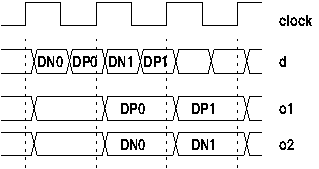
\includegraphics{iddr1}
            
            mode == "pfirst" - this is the same as above but there is an
            additional pipeline register inserted before the positive edge
            register. The two outputs thus capture +ve:-ve pairs in that order
            and both outputs are clocked on the +ve clock edge. There is an
            extra cycle of latency in this mode.
            
            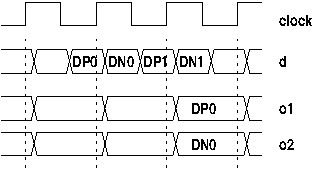
\includegraphics{iddr2}
            
            mode == "split" - input data is assigned to {\bf o1} on positive
            clock edges and to {\bf o2} on negative clock edges. The two outputs
            are thus in different (complementary) clock domains.
            
            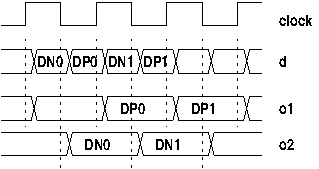
\includegraphics{iddr3}
            
            No input parameters may contain queue reads.
            
            Example code; input from a 2-channel DDR analog to digital
            converter -
            io.3pl
            \begin{lstlisting}[gobble=12, language=threepl]
               str(lvcmos33, "LVCMOS33");

               // package pins
               iopins(adc_clk_pin, lvcmos33, "str", "E17");
               iopins(adc_pins, lvcmos33, "[8]str",
                                   {"F2", "G2", "H2", "J2", "H1", "E1", "G1", "E2"});

               // ADC clock
               clock(adc_clk_in, frequency=100.0e6, loc=adc_clk_pin, ibufg=true);
               clock({global.adc_clk, adc_clk_raw}, frequency=100.0e6);
               clkdcm(clk0=adc_clk_raw <- clkin=adc_clk_in, clkfb=adc_clk);
               clockbufg(adc_clk <- adc_clk_raw);
               attributes(adc_clk, tnm="ADC_CLK");

               // ADC interface
               useclock(adc_clk);
               value({adc0, adc1}, "uint:8");
               input(adc_in, "uint:8", loc=adc_pins);
               iddr(adc0, adc1 <- adc_in,,, "nfirst");
            \end{lstlisting}
            
            Value variables {\bf adc0} and {\bf adc1} now 'point' to registers
            which are assigned ADC values on each positive edge of the clock,
            one from each channel.
            


        \subsubsection{idelay - input data delay}\label{sec:lpidelay}

            {\bf Library: xilinx/io.3pl}

            {\bf Prototype:} \\
            \vsp
            \begin{lstlisting}[gobble=12, language=threepl]
               global procedure
               idelay (
                   value(o)
                   <-
                   input(d),
                   int(delay),
                   clock(refclk),
                   value({ce, inc, rst}, "log"),
                   log(isclock)
               ) {}
            \end{lstlisting}

            {\bf Output parameters:} \\
            {\bf o} is the data output.

            {\bf Input parameters:} \\            
            {\bf d} is the data input.\\
            {\bf delay} gives a delay count.\\
            {\bf refclk} is a reference clock to control the delay.\\
            {\bf ce} is an optional clock enable for changing the delay.\\
            {\bf inc} is an optional direction control for changing the delay.\\
            {\bf rst} is an optional reset for the delay.\\
            {\bf isclock} should be true for a clock signal and false for a data
            signal.\\
         
            {\bf In-line target execution:} \\
            no

            {\bf description:} \\
            This procedure generates an input delay block.
            
            The data input {\bf d} is an input mode variable and must be a
            single bit.

            The output parameter {\bf o} is the delayed signal and is also a
            single bit.
            
            {\bf ce}, {\bf inc} and {\bf rst} inputs are used to change the
            delay value. These must be in the current clock domain.
            
            If input parameters {\bf delay} or {\bf ce} have an argument then
            the input parameter {\bf refclk} must be supplied with a clock whose
            frequency lies between 190.0MHz and 210.0MHz but is ideally 200MHz.
            If {\bf idelay()} is called more than once when {\bf variable} has
            an argument, then the same reference clock must be supplied to each
            call. Any calls to {\bf iodelay()} must also use the same reference
            clock.
            
            If input parameter {\bf ce} has no argument then the delay will be
            fixed. Input parameter {\bf delay} gives the required delay. The
            delay is $400 + 78 * delay$ pS for a reference clock frequency of
            200MHz. If {\bf delay} has no argument the delay count will be zero
            (giving $400$pS).
            
            If input parameter {\bf ce} has an argument then the delay will be
            variable. Input parameter {\bf delay} gives the initial delay count
            (default 0). The delay can be changed by asserting {\bf ce}. If {\bf
            inc} is true the delay will be incremented, otherwise it will be
            decremented. If {\bf rst} is asserted the delay will be changed back
            to the initial delay value. The clock domain of {\bf ce}, {\bf inc}
            and {\bf rst} is the current clock domain.
            
            Parameter {\bf isclock} describes the signal type which optimises
            the timing analyser for periodic or non-periodic signals.
            
            No input parameters may contain queue reads.
            
            Implementation note: this procedure will automatically create an
            IDELAYCTRL block on the first call to {\bf idelay()} that has a
            non-default delay. The Xilinx software will duplicate this across
            all locations where required. Xilinx recommend explicitly creating
            an IDELAYCTRL for each I/O region. This seems like hard work
            requiring a detailed floor plan and it is not clear why they suggest
            doing so.
            


        \subsubsection{iodelay - input/output data delay}\label{sec:lpiodelay}

            {\bf Library: xilinx/io.3pl}

            {\bf Prototype:} \\
            \vsp
            \begin{lstlisting}[gobble=12, language=threepl]
               global procedure
               iodelay (
                   value(dataout)
                   <-
                   input(idatain),
                   value(odatain),
                   log(variable),
                   int({idelay, odelay}),
                   clock(refclk),
                   value({t, ce, inc, rst}, "log")
               ) {}
            \end{lstlisting}

            {\bf Output parameters:} \\
            {\bf dataout} is the data output.

            {\bf Input parameters:} \\            
            {\bf idatain} is the data input from an IBUF (input mode variable).\\
            {\bf odatain} is the data input from OLOGIC.\\
            {\bf variable} specifies the type of input delay.\\
            {\bf idelay} gives the input delay count.\\
            {\bf odelay} gives the output delay count.\\
            {\bf refclk} is a reference clock to control the delays.\\
            {\bf t} is 3-state output control.\\
            {\bf ce} is an optional clock enable for changing the delay.\\
            {\bf inc} is an optional direction control for changing the delay.\\
            {\bf rst} is an optional reset for the delay.
        
            {\bf In-line target execution:} \\
            no

            {\bf description:} \\
            This procedure generates an input and output delay block.
            
            {\bf idatain} is an input mode variable and is the delay data
            source on input ({\bf t} is true). It must be one bit.

            {\bf odatain} is the delay data source on output ({\bf t} is false).
            This may be a CLB source ({\bf value} or {\bf static} mode variable)
            or the output of an ODDR block (output argument of oddr()). If this
            is a static mode variable it will be placed in an OLOGIC block. It must
            be a single bit.

            {\bf t} switches between input and output mode and must also control
            the output 3-state drive via an output mode variable with
            conditional assignment using {\bf t}.

            The output parameter {\bf o} is the delayed signal. It can be used
            directly or connected to an IDDR block (input argument to iddr())
            and must also be connected to an OBUFT (via an {\bf output} mode
            variable).

            If input parameter {\bf variable} is not given an argument then the
            input delay is the default fixed delay necessary for zero hold time
            on registered input data when no DCM is used. Arguments {\bf ce},
            {\bf inc} and {\bf rst} must be omitted.

            Input parameter {/bf refclk} must be supplied with a clock whose
            frequency lies between 190.0MHz and 210.0MHz but is ideally 200MHz.
            Multiple calls to {\bf iodelay()} must use the same reference clock.
            Any calls to {\bf idelay()} where parameter {\bf variable} has an
            argument must also use this same reference clock.

            If input parameter {\bf variable} has an argument whose value is
            false then the input delay will be fixed. Input parameter {\bf
            idelay} gives the required delay. The delay is $400 + 78 * delay$ pS
            for a reference clock frequency of 200MHz. If {\bf idelay} has no
            argument the delay count will be zero (giving $400$pS).

            If input parameter {\bf variable} has an argument whose value is
            true then the input delay will be variable. Input parameter {\bf
            idelay} gives the initial delay count (default 0). The delay can be
            changed by asserting {\bf ce}. If {\bf inc} is true the input delay
            will be incremented, otherwise it will be decremented. If {\bf rst}
            is asserted the input delay will be changed back to the initial
            delay value. The clock domain of {\bf ce}, {\bf inc} and {\bf rst}
            is the current clock domain.

            The output delay is set by {\bf odelay} and is $400 + 78 * delay$ pS
            for a reference clock frequency of 200MHz. If {\bf odelay} has no
            argument the delay count will be zero (giving $400$pS).

            No input parameters may contain queue reads.

            Implementation note: this procedure will automatically create an
            IDELAYCTRL block on the first call to {\bf iodelay()} that has a
            non-default delay. The Xilinx software will duplicate this across
            all locations where required. Xilinx recommend explicitly creating
            an IDELAYCTRL for each I/O region. This seems like hard work
            requiring a detailed floor plan and it is not clear why they suggest
            doing so.




        \subsubsection{iserdes - input deserialiser}\label{sec:lpiserdes}

            {\bf Library: xilinx/io.3pl}

            {\bf Prototype:} \\
            \vsp
            \begin{lstlisting}[gobble=12, language=threepl]
               global module
               iserdes (
                   value(q),
                   value({shiftout1, shiftout2}, "log")
                   <-
                   str(interface, "NETWORKING"),
                   log(master, true), log(ddr, true),
                   int(width),
                   clock({clk, clkb, oclk, oclkb, clkdiv}), value({din, ddlyin}),
                   value(bitslip, "log", false),
                   value({ce1, ce2}, "log"),
                   value({shiftin1, shiftin2, rst}, "log", false)
               ) {}
            \end{lstlisting}

            {\bf Output parameters:} \\
            see below.

            {\bf Input parameters:} \\            
            See below.
        
            {\bf In-line target execution:} \\
            no

            {\bf description:} \\
            A serial to parallel converter interface for the Xilinx
            ISERDES element. These may be used as a master-slave pair
            in DDR mode for output widths greater than 8.
            
            {\bf q} is the data output and must be of type "[n]bits:1"
            where 'n' is the output width. For a master ISERDES 'n' will be
            2, 3, 4, 5, 6, 7 or 8. For a slave ISERDES  'n' will be 2 for a
            data width of 10, or 6 for a data width of 14.
            
            {\bf shiftout1} and {\bf shiftout2} are connections to the
            slave ISERDES for widths 10 and 14.
            
            {\bf interface} selects the interface type which can be "MEMORY",
            "MEMORY\_DDR3", "MEMORY\_QDR", "OVERSAMPLE" or "NETWORKING" (default).
            
            {\bf master} selects master mode if true, or slave mode otherwise.
            Default is true (master mode)
            
            {\bf ddr} selects DDR mode if true, SDR mode if false.
            Default is true (DDR mode).
            
            {\bf width} is the data width.
            
            \begin{tabular}{| l | l | l |}
            \hline
                & networking          & memory \\
            \hline \hline
            sdc & 2, 3, 4, 5, 6, 7, 8 & not allowed \\ \hline
            ddr & 4, 6, 8, 10, 14(*)  & 4           \\ \hline
            \end{tabular}

            (* ddr mode networking interface width 14 not allowed for XC5V
            ISERDES\_NODELAY).
            
            Where a master-slave pair are used for a width of 10 or 14 that
            width argument must be the full width for both modules of the pair
            even though the data outputs {\bf q} are smaller, i.e. for a data
            width of 14 both ISERDES modules will have a width argument 14 even
            though the master has an 8-bit output and the slave a 6-bit output.
            
            {\bf clk} the main or only serial data input clock.
            
            {\bf clkb} second serial data input clock for MEMORY\_QDR mode. For
            other modes this should be the inverted main clock.
            
            {\bf oclk} is the strobe clock for memory mode.
            
            {\bf oclkb} is the inverted {\bf oclk}.
            
            {\bf clkdiv} is the frame clock input which must have a frequency
            which is serial clock frequency divided by the serial frame
            length.
            
            {\bf din} is the serial data input direct from an input pad. {\bf
            ddlyin} is the serial data input from an IDELAY element. One and
            only one of these should be given an argument.
            
            {\bf bitslip} when asserted increases the deserialiser frame
            delay by one bit position.
            
            {\bf ce1} is the clock enable for {\bf clk}.
            
            {\bf ce2} is the clock enable for {\bf clkb}.
            
            {\bf shiftin1}, {\bf shiftin2} are connections from a
            master ISERDES to a slave ISERDES for widths 10 and 14.
            
            {\bf rst} is a reset signal.
            
            See the Xilinx documentation for details on the use of this
            element.





        \subsubsection{oddr - output double data rate interface}\label{sec:lpoddr}

            {\bf Library: xilinx/io.3pl}

            {\bf Prototype:} \\
            \vsp
            \begin{lstlisting}[gobble=12, language=threepl]
               global procedure
               oddr (
                   value(o)
                   <-
                   value(i1),
                   value(i2),
                   value({ce, s, r}, "log")
               ) {}
            \end{lstlisting}

            {\bf Output parameters:} \\
            {\bf o} is the DDR data output.

            {\bf Input parameters:} \\            
            {\bf i1} is the -ve edge data input.\\
            {\bf i2} is the +ve edge data input.\\
            {\bf ce} is an optional clock enable.\\
            {\bf r} is an optional reset.\\
            {\bf s} is an optional set.
        
            {\bf In-line target execution:} \\
            no

            {\bf description:} \\
            This procedure creates an output DDR (Double Data Rate) interface.
            
            The argument to output parameter {\bf o} would usually also be
            passed as the third argument to an {\bf output()} inbuilt procedure
            call to drive output buffers.
            
            Input parameters {\bf i1} and {\bf i2} are registered on the
            current clock positive edge. The data from i1 appears at the
            output o following a positive clock edge and the data from
            i2 appears at the output o on the next negative clock edge.

            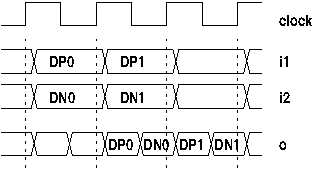
\includegraphics{oddr}
            
            The clock used for the DDR registers is the current clock.
            
            {\bf ce} is an optional clock enable.
            
            {\bf r} can be used to clear the output register and {\bf s} to set
            it to all ones. These can be synchronous or asynchronous depending
            on attribute SRTYPE and are synchronous by default.
            
            No input parameters may contain queue reads.
            
            Example; DDR output, including a clock -

            \begin{lstlisting}[gobble=12, language=threepl]
               str(lvcmos33, "LVCMOS33");

               // package pins
               iopins(out_pins, lvcmos33, "[8]str",
                                   {"F2", "G2", "H2", "J2", "H1", "E1", "G1", "E2"});
               iopins(ddr_clk_pin, lvcmos33, "str", "E17");

               static({out0, out1}, "uint:8");
               
               out0 <- .....;
               out1 <- .....;
               
               value(ddr, "uint:8");
               value(ddr_clk, "log");
               
               oddr(ddr <- out0, out1);
               oddr(ddr_clk <- false, true);
               
               output(,, ddr, loc=out_pins);
               output(,, ddr_clk, loc=ddr_clk_pin);
            \end{lstlisting}
            
            Forwarding a clock via a DDR output is a scheme suggested by
            Xilinx (XAPP 853, p9) to maintain matching phase.



        \subsubsection{oserdes - output serialiser/deserialiser}\label{sec:lposerdes}

            {\bf Library: xilinx/io.3pl}

            {\bf NOT YET IMPLEMENTED!}




    \subsection{library functions}
    
        None.





    \subsection{library classes}
    
        None.


\pagebreak

\section{Xilinx VirtexII Pro MGT library - xilinx/mgt.3pl}

    \index{library!xilinx/mgt.3pl}
    This library provide a simple 16 bit interface to a VirtexII Pro
    Multi-Gigabit Transceiver (referred to as an MGT or Rocket).
    
    This library must be incorporated by using a module statement, e.g. -
    \begin{lstlisting}[gobble=4, language=threepl]
       module "xilinx/mgt.3pl"
    \end{lstlisting}
    
    The global structures {\bf mgt\_16}, {\bf mgt\_16\_e} and {\bf mgt\_16\_ee}
    are created. They are defined as follows -

    \begin{lstlisting}[gobble=4, language=threepl]
       struct(global.gt_16,
           data,   "bits:16",  // data
           k,      "log",      // true if top 8 bits of data form a K-character
           contin, "log"       // this is a continuation word
       );
    \end{lstlisting}

    \begin{lstlisting}[gobble=4, language=threepl]
       struct(global.gt_16_e,
           data,   "bits:16",  // data
           k,      "log",      // true if top 8 bits of data form a K-character
           first,  "log",      // previous word was an idle
           error,  "log"       // disparity error or not-in-table error
       );
    \end{lstlisting}

    \begin{lstlisting}[gobble=4, language=threepl]
       struct(global.gt_16_ee,
           data,       "bits:16",  // data
           k,          "log",      // true if top 8 bits of data form a K-character
           first,      "log",      // previous word was an idle
           disperr,    "[2]log",   // disparity errors
           niterr,     "[2]log"    // not-in-table errors
       );
    \end{lstlisting}

    {\bf mgt\_16} is used for input data. {\bf mgt\_16\_e} and
    {\bf mgt\_16\_ee} are used for output data, the former providing a simpler
    error indication than the latter.
    
    The global structure {\bf ds16} is also used and it is created in
    {\bf stdlib.3pl}. It is 
    \begin{lstlisting}[gobble=4, language=threepl]
       struct(global.ds16,
           data,   "bits:16",  // data
           k,      "log"       // true if top 8 bits of data form a K-character
       );
    \end{lstlisting}


    \subsection{library modules}

        \subsubsection{gt\_custom\_16 - a 16-bit Rocket high-speed serial I/O channel}\label{sec:lmgtcustom16}

            {\bf Library: xilinx/mgt.3pl}

            {\bf Prototype:} \\
            \vsp
            \begin{lstlisting}[gobble=12, language=threepl]
               global module
                   gt_custom_16 (
                       queue(out),
                       clock(ruclk),
                       value(rxdiag, "[5]log"),
                       value(txdiag, "[2]log")
                       <-
                       str({loc, txp_pin, txn_pin, rxp_pin, rxn_pin, clkp_pin, clkn_pin}),
                       float(freq),         // MGT base frequency
                       queue(in),
                       int(run_length),
                       value(reset, "log"),
                       int(tx_diff_ctrl, 500),
                       int(tx_preemphasis, 0),
                       value(loopback, "uint:2", 0),
                       log(los_fsm)
                   ) {}
            \end{lstlisting}

            {\bf Output parameters:} \\
            {\bf out} is the data output.\\
            {\bf ruclk} is the user interface clock.\\
            {\bf rxdiag} provides five diagnostic receiver signals.\\
            {\bf txdiag} provides two diagnostic transmitter signals.

            {\bf Input parameters:} \\
            {\bf loc} gives the MGT location coordinates.\\
            {\bf txp\_pin} specifies the transmitter positive output pin.\\
            {\bf txn\_pin} specifies the transmitter negative output pin.\\
            {\bf rxp\_pin} specifies the receiver positive input pin.\\
            {\bf rxn\_pin} specifies the receiver negative input pin.\\
            {\bf clkp\_pin} specifies the clock input positive pin.\\
            {\bf clkn\_pin} specifies the clock input negative pin.\\
            {\bf freq} is the parallel input and output data frequency.\\
            {\bf in} is the data input.\\
            {\bf run\_length} is the maximum data run length.\\
            {\bf reset} when true resets the initialisation flag.\\
            {\bf tx\_diff\_ctrl} specifies the differential output voltage.\\
            {\bf tx\_preemphasis} specifies the transmitter preemphasis.\\
            {\bf loopback} when true connects the MGT in loopback mode.\\
            {\bf los\_fsm} when true connects enables the MGT loss-of-sync FSM.

            {\bf Description:} \\
            This module provides a simple interface to procedure
            {\bf mgt()} \autorefph{sec:lpmgt}, in this library.
            It creates both an input and an output interface to the
            VirtexII Pro MGT. The data width is 16 bit. A custom protocol
            is used. 
            
            The particular MGT is selected by the first 7 input arguments.
            The {\bf loc} does not seem to be required but the transmitter pin,
            receiever pin and clock pin pairs must be provided. The following
            combinations apply to the XC2VP4 -           
            
            \begin{tabular}{| l || r | r | r | r |}
            \hline
            MGT      & TXP  & TXN  & RXP  & RXN  \\
            location & pin  & pin  & pin  & pin  \\
            \hline
            \hline
            GT\_X0Y0 & AB8  & AB7  & AB9  & AB10 \\
            \hline
            GT\_X0Y1 & A8   & A7   & A9   & A10  \\
            \hline
            GT\_X1Y0 & AB14 & AB13 & AB15 & AB16 \\
            \hline
            GT\_X1Y1 & A14  & A13  & A15  & A16  \\
            \hline
            \end{tabular}
            
            and for the XC2VP40 -

            \begin{tabular}{| l || r | r | r | r |}
            \hline
            MGT      & TXP  & TXN  & RXP  & RXN  \\
            location & pin  & pin  & pin  & pin  \\
            \hline
            \hline
            GT\_X0Y0 & ap32 & ap33 & ap31 & ap30 \\
            \hline
            GT\_X0Y1 &  a32 &  a33 &  a31 &  a30 \\
            \hline
            GT\_X1Y0 & ap28 & ap29 & ap27 & ap26 \\
            \hline
            GT\_X1Y1 &  a28 &  a29 &  a27 &  a26 \\
            \hline
            GT\_X2Y0 & ap20 & ap21 & ap19 & ap18 \\
            \hline
            GT\_X2Y1 &  a20 &  a21 &  a19 &  a18 \\
            \hline
            GT\_X3Y0 & ap16 & ap17 & ap15 & ap14 \\
            \hline
            GT\_X3Y1 &  a16 &  a17 &  a15 &  a14 \\
            \hline
            GT\_X4Y0 &  ap8 &  ap9 &  ap7 &  ap6 \\
            \hline
            GT\_X4Y1 &   a8 &   a9 &   a7 &   a6 \\
            \hline
            GT\_X5Y0 &  ap4 &  ap5 &  ap3 &  ap2 \\
            \hline
            GT\_X5Y1 &   a4 &   a5 &   a3 &   a2 \\
            \hline
            \end{tabular}
            
            {\bf freq} is an immediate floating point value which specifies the
            MGT base frequency in Hz. For 2.5GHz serial the base frequency
            is 125.0MHz (serial rate divided by 20).
            
            Input parameter {\bf in} is the input data queue for the transmitter.
            If the transmitter is not used the argument is omitted. The type is
            either the struct {\bf ds16} (defined in stdlib.3pl) or the struct
            {\bf gt\_16}. The most significant byte of the word may be a
            K-character, which is signified by setting field {\bf k} true. The
            byte must be one of the allowed K-characters (this is not checked!).
            For type {\bf gt\_16} the {\bf contin} field should be true if this
            word is a continuation word, i.e. it is not the first word in a
            block. This ensures that despite the run length constraint (see
            Input parameter {\bf run\_length} below) a block will not be split
            by inserted idles. At the receiving end the first word following an
            idle can reset a block boundary.

            Input parameter {\bf run\_length} is an immediate integer which
            specifies the maximum contiguous data run for the transmitter. If
            data input is continuously available such that this length would be
            exceeded (and the data {\bf contin} field is not true - see above)
            then an idle sequence is inserted in the output stream. When no data
            are available for transmission a continuous stream of idles is
            transmitted. These idles are used by the receiver to lock initially
            and to continue checking that lock is maintained. If receiver lock
            is lost then lock can only be regained at the next idle. In the
            custom protocol used in this interface the idle sequence is a single
            16-bit word containing a comma byte. If no argument is supplied
            to parameter {\bf run\_length} then idles will only be inserted
            when the input queue is unavailable.

            Input parameter {\bf reset} is used to clear the initialisation flag
            and execute initialisation process. This initialisation process
            expects to receive idles only for 6 seconds without error. If an
            error or a non-idle word is received in this time the received is
            reset and a further wait ensues. When 6 seconds of idles have been
            received the initialisation flag is set and the channel can now receive
            data. The initialisation process occurs immediately following
            configuration of the FGA. Clearly during this initialisation, and any
            others that are explicitly induced, the transmitter must be sending
            idles.

            Input parameter {\bf tx\_diff\_ctrl} specifies the differential
            output voltage and is 500 by default. Values are 400, 500, 600, 700
            or 800 which is the differential voltage in mV. The peak-to-peak
            voltage is twice this figure.

            Input parameter {\bf tx\_preemphasis} specifies the transmitter
            preemphasis and is 0 by default. values are 0 (10\%), 1 (20\%),
            2 (25\%) or 3 (33\%).

            Input parameters {\bf tx\_diff\_ctrl} and {\bf tx\_preemphasis} control
            the transmitter output waveforms to correct for different cable types
            and lengths. Any changes to the default values are usually done
            empirically based on the measured error rate.

            Input parameter {\bf loopback} is an immediate integer which specifies
            the loopback mode. If the argument is omitted or is 0, operation is
            normal, i.e. loopback is not connected. Value 1 specifies internal
            parallel mode. Value 2 specifies internal serial mode.
            
            Input parameter {\bf los\_fsm} controls the use of the MGT loss-of-sync
            finite state machine which detects when sync is held/lost. If the argument
            to this is false then {\bf rxdiag[3]} will only indicate if channel
            initialisation was successful. If {\bf los\_fsm} is true then  {\bf
            rxdiag[3]} will be asserted when the receiver has been successfully
            initialised and remain asserted while sync is OK.

            Output parameter {\bf out} is the output data queue for the receiver.
            If the receiver is not used the argument is omitted. The type can be
            struct {\bf ds16}, struct {\bf gt\_16\_e} or  struct {\bf
            gt\_16\_ee} depending on the level of error
            detail required. The {\bf k} field in each case is true if the most
            significant byte of the received word contains a K-character.
            For {\bf gt\_16\_e} or  {\bf gt\_16\_ee} the {\bf first} field
            is true then this word follows an idle, which information may be
            used to reset a block boundary. {\bf Important note - the output
            queue must not block! The destination module must read it at a rate
            that precludes it ever becoming full, if necessary reading it to
            null. Generally the read clock domain must have an equal or higher
            frequency than the user interface clock {\bf ruclk}, but this may be
            relaxed if it is known that the serial data source has a guaranteed
            maximum data rate that would allow a lower queue read clock domain.}
            For {\bf gt\_16\_e} the {\bf error} field is true if either byte
            exhibits a disparity error or not-in-table error. {\bf gt\_16\_ee}
            provides each of these errors separately for each byte.
            
            A word in which a disparity error or a not-in-table error occurs is
            written to the output queue but the error field is true. If the top
            byte of a word is a K-character the {\bf k} field is true.

            Output parameter {\bf ruclk} is the user interface clock at the base
            frequency.
            
            Output parameter {\bf rxdiag} provides five diagnostic outputs for the
            receiver. These are -
            \blist
            \item   diag[0] - rxcommadet, which is true when a positive or
                    negative comma is being received
            \item   diag[1] - rxdisperr[0] or rxnotintable[0], which is true
                    when a disparity error or a not-in-table error is
                    flagged for the current upper byte of the 16-bit output
            \item   diag[2] - rxdisperr[1] or rxnotintable[1], which is true
                    when a disparity error or a not-in-table error is
                    flagged for the current lower byte of the 16-bit output
            \item   diag[3] - is true if the receiver is synchronised, as
                    indicated by the receiver synchronisation FSM \footnote{if
                    parameter los\_fsm is true.} , and the
                    initialisation flag is high
            \item   diag[4] - is true if the receiver is receiving idles
            \blend
            These outputs might be connected to status LEDs to indicate that the
            receiver is locked and functioning correctly. {\bf diag[0]} will be true
            while the receiver is receiving idles but will be false when data are
            received.

            Output parameter {\bf txdiag} provides two diagnostic outputs for the
            transmitter. These are -
            \blist
            \item   diag[0] - is true if the transmitter is sending idles
            \item   diag[1] - is true if the transmitter is sending a word in which
                    the top byte is a control character
            \blend


    \subsection{library procedures}

        \subsubsection{mgt - create an MGT high-speed serial I/O channel}\label{sec:lpmgt}

            {\bf Library: xilinx/mgt.3pl}

            {\bf Prototype:} \\
            \vsp
            \begin{lstlisting}[gobble=12, language=threepl]
               global procedure
               mgt (
                   // outputs
                   value(rxdata),
                   value(rxchariscomma, "[]log"),
                   value(rxcharisk, "[]log"),
                   value(rxcommadet, "log"),
                   value(rxlossofsync, "uint:2"),
                   value(rxnotintable, "[]log"),
                   value(rxbufstatus, "[2]log"),
                   value(rxcheckingcrc, "log"),
                   value(rxclkcorcnt, "uint:3"),
                   value(rxcrcerr, "log"),
                   value(rxdisperr, "[]log"),
                   value(rxrealign, "log"),
                   value(rxrecclk, "log"),
                   value(rxrundisp, "[]log"),
                   value(txbuferr, "log"),
                   value(txkerr, "[]log"),
                   value(txrundisp, "[]log"),
                   value(chbondo, "[4]log"),
                   value(chbonddone, "log")
                   <-
                   // attributes
                   str(loc),
                   str(txn_pin),
                   str(txp_pin),
                   str(rxn_pin),
                   str(rxp_pin),
                   log(align_comma_msb),
                   int(chan_bond_limit),
                   str(chan_bond_mode),
                   int(chan_bond_offset),
                   log(chan_bond_one_shot),
                   int(chan_bond_seq_1_1),
                   int(chan_bond_seq_1_2),
                   int(chan_bond_seq_1_3),
                   int(chan_bond_seq_1_4),
                   int(chan_bond_seq_2_1),
                   int(chan_bond_seq_2_2),
                   int(chan_bond_seq_2_3),
                   int(chan_bond_seq_2_4),
                   log(chan_bond_seq_2_use),
                   int(chan_bond_seq_len),
                   int(chan_bond_wait),
                   log(clk_cor_insert_idle_flag),
                   log(clk_cor_keep_idle),
                   int(clk_cor_repeat_wait),
                   int(clk_cor_seq_1_1),
                   int(clk_cor_seq_1_2),
                   int(clk_cor_seq_1_3),
                   int(clk_cor_seq_1_4),
                   int(clk_cor_seq_2_1),
                   int(clk_cor_seq_2_2),
                   int(clk_cor_seq_2_3),
                   int(clk_cor_seq_2_4),
                   log(clk_cor_seq_2_use),
                   int(clk_cor_seq_len),
                   log(clk_correct_use),
                   int(comma_10b_mask),
                   int(crc_end_of_pkt),
                   str(crc_format),
                   int(crc_start_of_pkt),
                   log(dec_mcomma_detect),
                   log(dec_pcomma_detect),
                   log(dec_valid_comma_only),
                   int(mcomma_10b_value),
                   log(mcomma_detect),
                   int(pcomma_10b_value),
                   log(pcomma_detect),
                   int(ref_clk_v_sel),
                   log(rx_crc_use),
                   int(rx_data_width),
                   log(rx_decode_use),
                   int(rx_los_invalid_incr),
                   int(rx_los_threshold),
                   log(rx_loss_of_sync_fsm),
                   log(serdes_10b),
                   int(termination_imp),
                   int(tx_crc_force_value),
                   log(tx_crc_use),
                   int(tx_data_width),
                   int(tx_diff_ctrl),
                   int(tx_preemphasis),
                   // Inputs
                   value(chbondi, "[4]log"),
                   value(enchansync, "log"),
                   value(enmcommaalign, "log"),
                   value(enpcommaalign, "log"),
                   value(loopback, "uint:2"),
                   value(powerdown, "log"),
                   value(refclk, "log"),
                   value(refclk2, "log"),
                   value(brefclk, "log"),
                   value(brefclk2, "log"),
                   value(refclksel, "log"),
                   value(rxpolarity, "log"),
                   value(rxreset, "log"),
                   clock(rxusrclk),
                   clock(rxusrclk2),
                   value(txbypass8b10b, "[]log"),
                   value(txchardispmode, "[]log"),
                   value(txchardispval, "[]log"),
                   value(txcharisk, "[]log"),
                   value(txdata),
                   value(txforcecrcerr, "log"),
                   value(txinhibit, "log"),
                   value(txpolarity, "log"),
                   value(txreset, "log"),
                   clock(txusrclk),
                   clock(txusrclk2)

               ) {}
            \end{lstlisting}

            {\bf Output parameters:} \\
            See Xilinx documentation.

            {\bf Input parameters:} \\
            See Xilinx documentation.

            {\bf In-line target execution:} \\
            no

            {\bf description:} \\
            This procedure creates an MGT high speed serial I/O channel.
            For a simpler interface
            see {\bf gt\_custom\_16} \autorefph{sec:lmgtcustom16} above.



    \subsection{library functions}
    
        None.


    \subsection{library classes}
    
        None.


\pagebreak

\section{Xilinx netlist postprocessing module - xilinx/postprocess.3pl}\label{ch:pp}

    \index{library!xilinx/postprocess.3pl}
    This module converts the EDIF netlist produced by 3PL to a configuration
    file. It has a single procedure.
    
    This library must be incorporated by using a postmodule statement, e.g. -
    \begin{lstlisting}[gobble=4, language=threepl]
       postmodule ("xilinx/postprocess.3pl");
    \end{lstlisting}
    
    See \autorefph{sec:mpfcdecl} and \autorefph{sec:xpp}.
    
    More than one postprocessing module can be specified in which case an
    additional integer argument can be supplied to specify ordering. If omitted
    the order in which the modules have been added to the list will be the order
    of execution. Thus far only this module has been used.
    


    \subsection{library modules}

        None.



    \subsection{library procedures}

        \subsubsection{postprocess - post-process the netlist file}\label{sec:lppostprocess}

            {\bf Prototype:} \\
            \vsp
            \begin{lstlisting}[gobble=12, language=threepl]
                global procedure
                postprocess(
                    str(rname),
                    str(tool),
                    float(minver, 1.0),
                    float(maxver, 9999.0)
                ) {}
            \end{lstlisting}



            {\bf Output parameters:} \\
            
            None.

            {\bf Input parameters:} \\
            \begin{tabular}{| l | l | l | l |}
            \hline
                            & mode      & type   & \\
            \hline \hline
            {\bf rname}     & immediate & str    & optional file name for recipe file \\ \hline
            {\bf tool}      & immed     & str    & "ise" or "vivado" \\ \hline
            {\bf minver}    & immediate & float  & minimum version number  \\ \hline
            {\bf maxver}    & immediate & float  & maximum version number \\ \hline
            \end{tabular}

            {\bf In-line target execution:} \\
            no

            {\bf description:} \\
            This procedure executes the Xilinx place-and-route tools to
            generate the configuration bit file from the EDIF netlist file
            produced by 3PL. To do this it executes the Xilinx tools
            on the host CPU via calls to exec().
            
            {\bf rname} optional and is the name of a file containing a recipe
            of commands. If supplied it overrides the recipe file specified by
            directive {\bf postProcessRecipe}. Recipe files
            {\bf ise\_cpld.cmd}, {\bf ise\_fpga.cmd}, {\bf ise\_xflow.cmd}
            and {\bf vivado.tcl} are available in the directory
            containing postprocess.3pl.
            
            {\bf tool} "ise" or "vivado" must be supplied and specifies the
            main place-and-route tool to be used.
            
            If directives {\bf XILINX\_ISE} or {\bf XILINX\_VIVADO} are supplied
            (as appropriate to the platform) then this specifies the specific
            path of the place-and-route tool to execute. Otherwise the path
            specified by directive {\bf XILINX} will be used along with  {\bf
            minver} and {\bf maxver} to select the specific version of the ISE
            or Vivado software. The highest version \verb'>=' minver and
            \verb'<=' maxver will be used.


            if directive {\bf postProcessAppendFile} exists it specifies
            a file to append to the bit file, usually a .info file

            if directive {\bf postProcessCompress} exists and is true
            the bit file will be compressed.

            If directive {\bf postProcessFilter} exists it specifies that the
            standard output from the place-and-route tools should be filtered.
            Values may be -
            \blist
            \item   "error" - lines starting with "ERROR" are retained
            \item   "critical" - the above plus lines starting with "CRITICAL" are
                    retained
            \item   "warning" - the above plus lines starting with "WARNING" are
                    retained
            \item   "info" - the above plus lines starting with "INFO" are
                    retained
            \blend
            any other values being ignored. If this directive is not defined or
            has an invalid value then no filtering is applied.
    
    
    


    \subsection{library functions}
    
        None.


    \subsection{library classes}
    
        None.


\pagebreak

\section{Embedded PowerPC Interface Library - xilinx/ppc405lib.3pl}
\label{chap:lmppc405lib}

    {\bf This library has never been used in earnest so its functionality has not
    been tested!}

    \index{library!xilinx/ppc405lib.3pl}
    {\bf This library provides an instantiation of an embedded PowerPC.}
    
    This library must be incorporated by using a {\bf module} statement -
    \begin{lstlisting}[gobble=4, language=threepl]
       module "xilinx/ppc405lib.3pl"
    \end{lstlisting}




    \subsection{library modules}
    
    None.



    \subsection{library procedures}

         \subsubsection{ppc405 - a PPC405}\label{sec:lpppc405}

            {\bf Library: xilinx/ppc405lib.3pl}

            {\bf Prototype:} \\
            \vsp
            \begin{lstlisting}[gobble=12, language=threepl]
               global procedure
               ppc405 (
                   value({ C405CPMCORESLEEPREQ, C405CPMMSRCE, C405CPMMSREE, C405CPMTIMERIRQ,
                           C405CPMTIMERRESETREQ, C405DBGMSRWE, C405DBGSTOPACK,
                           C405DBGWBCOMPLETE, C405DBGWBFULL, C405DCRREAD, C405DCRWRITE,
                           C405JTGCAPTUREDR, C405JTGEXTEST, C405JTGPGMOUT, C405JTGSHIFTDR,
                           C405JTGTDO, C405JTGTDOEN, C405JTGUPDATEDR, C405PLBDCUABORT,
                           C405PLBDCUCACHEABLE, C405PLBDCUGUARDED, C405PLBDCUREQUEST,
                           C405PLBDCURNW, C405PLBDCUSIZE2, C405PLBDCUU0ATTR,
                           C405PLBDCUWRITETHRU, C405PLBICUABORT, C405PLBICUU0ATTR,
                           C405RSTCHIPRESETREQ, C405RSTCORERESETREQ, C405RSTSYSRESETREQ,
                           C405TRCCYCLE, C405PLBICUREQUEST, C405TRCTRIGGEREVENTOUT,
                           C405XXXMACHINECHECK, DSOCMBRAMEN, DSOCMBUSY, ISOCMBRAMEN,
                           ISOCMBRAMEVENWRITEEN, ISOCMBRAMODDWRITEEN, C405PLBICUCACHEABLE}, "log"),
                   value(C405DBGWBIAR, "bits:30"),
                   value(C405DCRABUS, "bits:10"),
                   value(C405DCRDBUSOUT, "bits:32"),
                   value(C405PLBDCUABUS, "bits:32"),
                   value(C405PLBDCUBE, "bits:8"),
                   value(C405PLBDCUPRIORITY, "uint:2"),
                   value(C405PLBDCUWRDBUS, "bits:64"),
                   value(C405PLBICUABUS, "uint:30"),
                   value(C405PLBICUPRIORITY, "uint:2"),
                   value(C405PLBICUSIZE, "uint:2"),
                   value(C405TRCEVENEXECUTIONSTATUS, "uint:2"),
                   value(C405TRCODDEXECUTIONSTATUS, "uint:2"),
                   value(C405TRCTRACESTATUS, "uint:4"),
                   value(C405TRCTRIGGEREVENTTYPE, "uint:11"),
                   value(DSOCMBRAMABUS, "uint:22"),
                   value(DSOCMBRAMBYTEWRITE, "[4]log"),
                   value(DSOCMBRAMWRDBUS, "bits:32"),
                   value(ISOCMBRAMRDABUS, "uint:21"),
                   value(ISOCMBRAMWRABUS, "uint:21"),
                   value(ISOCMBRAMWRDBUS, "bits:32")
                   <-
                   int({XLOC, YLOC}),
                   clock({ BRAMDSOCMCLK, BRAMISOCMCLK, CPMC405CLOCK, PLBCLK}),
                   value({ CPMC405CORECLKINACTIVE, CPMC405CPUCLKEN, CPMC405JTAGCLKEN, 
                           CPMC405TIMERCLKEN, CPMC405TIMERTICK, DBGC405DEBUGHALT,
                           DBGC405EXTBUSHOLDACK, DBGC405UNCONDDEBUGEVENT, DCRC405ACK, 
                           EICC405CRITINPUTIRQ, EICC405EXTINPUTIRQ, JTGC405BNDSCANTDO,
                           JTGC405TCK, JTGC405TDI, JTGC405TMS, JTGC405TRSTNEG,
                           MCBCPUCLKEN, MCBJTAGEN, MCBTIMEREN, MCPPCRST,
                           PLBC405DCUADDRACK, PLBC405DCUBUSY, PLBC405DCUERR, 
                           PLBC405DCURDDACK, PLBC405DCUSSIZE1, PLBC405DCUWRDACK,
                           PLBC405ICUADDRACK, PLBC405ICUBUSY, PLBC405ICUERR, 
                           PLBC405ICURDDACK, PLBC405ICUSSIZE1, RSTC405RESETCHIP, 
                           RSTC405RESETCORE, RSTC405RESETSYS, TIEC405DETERMINISTICMULT,
                           TIEC405DISOPERANDFWD, TIEC405MMUEN, TRCC405TRACEDISABLE,
                           TRCC405TRIGGEREVENTIN}, "log"),
                   value(BRAMDSOCMRDDBUS, "bits:32"),
                   value(BRAMISOCMRDDBUS, "bits:64"),
                   value(DCRC405DBUSIN, "bits:32"),
                   value(DSARCVALUE, "uint:8"),
                   value(DSCNTLVALUE, "uint:8"),
                   value(ISARCVALUE, "uint:8"),
                   value(ISCNTLVALUE, "uint:8"),
                   value(PLBC405DCURDDBUS, "bits:64"),
                   value(PLBC405DCURDWDADDR, "uint:3"),
                   value(PLBC405ICURDDBUS, "bits:64"),
                   value(PLBC405ICURDWDADDR, "uint:3"),
                   value(TIEDSOCMDCRADDR, "uint:8"),
                   value(TIEISOCMDCRADDR, "uint:8")
               ) {}
            \end{lstlisting}

            {\bf Output parameters:} \\
            See Xilinx documentation.

            {\bf Input parameters:} \\
            See Xilinx documentation.

            {\bf description:} \\
            This procedure creates an instance of a PowerPC 405 core.
            For a simpler interface see procedure {\bf ppcbr} \autorefph{sec:lpppcbr}
            above.






    \subsection{library functions}
    
    None.




    \subsection{library classes}
    
        None.


\pagebreak

\section{Embedded PowerPC Interface Library - xilinx/ppclib.3pl}
\label{chap:lmppclib}

    \index{library!xilinx/ppclib.3pl}
    {\bf This library provides a way of instantiating an embedded PowerPC. The
    library was under development but work on it has ceased. Its functionality has
    not been tested!}
    
    This library must be incorporated by using a {\bf module} statement -
    \begin{lstlisting}[gobble=4, language=threepl]
       module "xilinx/ppclib.3pl"
    \end{lstlisting}



    \subsection{library modules}
    
    None.



    \subsection{library procedures}

         \subsubsection{ppcbr - a PPC405 with OCM}\label{sec:lpppcbr}

            {\bf Library: xilinx/ppclib.3pl}

            {\bf Prototype:} \\
            \vsp
            \begin{lstlisting}[gobble=12, language=threepl]
               global module
               ppcbr (
                   var({iramp, dramp0, dramp1, dramp2, dramp3}, "->")
                   <-
                   int({imsk, dmsk}),
                   log({iramea, dramea}),
                   value({cpuclken, cpureset}, "log")
               ) {}
            \end{lstlisting}

            {\bf Output parameters:} \\
            {\bf iramp} pointer to 64 bit instruction RAM\\
            {\bf dramp0} pointer to data RAM byte 0 (most sig) \\
            {\bf dramp1} pointer to data RAM byte 1 \\
            {\bf dramp2} pointer to data RAM byte 2 \\
            {\bf dramp3} pointer to data RAM byte 3 (least sig)

            {\bf Input parameters:} \\            
            {\bf imsk} instruction memory size (bytes) in K - each 2K takes a
                       block RAM - must be 4, 8, 16, 32, 64 or 128\\           
            {\bf dmsk} data memory size (bytes) in K - each 2K takes a block RAM -
                       must be 2, 4, 8, 16, 32 or 64\\
            {\bf iramea} true if instruction ram 2nd port required for external
                         access\\
            {\bf dramea} true if data ram 2nd port required for external access\\
            {\bf cpuclken} enable CPU core clock\\
            {\bf cpureset} reset the CPU - this should be raised for a clock cycle\\

            {\bf description:} \\
            This procedure creates an interface to an embedded PowerPC 405. It
            uses on-chip block RAM for separate instruction and data memory.
            Both memories are located at address 0. The memory management is
            disabled. Pointers to the memories are available as output
            parameters to enable access via the second RAM port.
            This procedure calls {\bf ppc405} \autorefph{sec:lpppc405} above
            to create the PPC instance.
    




    \subsection{library functions}
    
        None.



    \subsection{library classes}
    
        None.




\pagebreak

\section{Zynq ARM processor interface Library - xilinx/zynq\_axi.3pl}
\label{chap:lmzynqaxilib}

    \index{library!xilinx/zynq\_axi.3pl}
    This library instantiates a Zynq CPU and provides interfaces to
    the two general purpose memory-mapped slave buses and the four
    high performance DMA master buses. It also connects the DDR RAM
    and general purpose I/O pins to the CPU.
    
    This library must be incorporated by using a {\bf source} statement -
    \begin{lstlisting}[gobble=4, language=threepl]
       source "xilinx/zynq\_axi.3pl"
    \end{lstlisting}

    however xilinx/zynq\_axi.3pl is already included in board header files -\\
    boards/avnet/microzed\_7010.3pl\\
    boards/avnet/microzed\_7020.3pl\\
    boards/digilent/zybo.3pl
    
    Code to create the interface to the CPU must be executed as a trailer module
    by -
    
    \begin{lstlisting}[gobble=4, language=threepl]
        trailermodule ("zynq processor") {
            zynq_ps();
        }
    \end{lstlisting}
    and this is also incorporated in the header files listed above.

    Application code only needs to incorporate the board header file
    and create an instance of the CPU interface, e.g. -

    \begin{lstlisting}[gobble=4, language=threepl]
        module "boards/avnet/microzed_7010.3pl"

        class(cpu, cpu_api());
    \end{lstlisting}
    The CPU\_API class is documented in
    \autorefph{chap:lmxilcpulib} {\bf FPGA to CPU interface Library
    - xilinx/cpu.3pl}. This library can also be used by FPGA boards
    which have a USB serial interface to a host computer.
   
    Since cpu.3pl is included via a source statement its code shares the scope
    of this library, UART\_CPU. Thus it can call the modules, functions and
    procedures therin.
    
    {\bf cpu.3pl} defines a class {\bf CPU\_API()} which provides the following
    class procedures for data transfer between FPGA and CPU - \\
        \hspace*{1cm}{\bf read()} generic read \autorefph{sec:lpcpurd} \\
        \hspace*{1cm}{\bf write()} generic write \autorefph{sec:lpcpuwr} \\
        \hspace*{1cm}{\bf read\_memory()} memory read \autorefph{sec:lpcpurdmem} \\
        \hspace*{1cm}{\bf read\_queue()} queue read \autorefph{sec:lpcpurdqueue} \\
        \hspace*{1cm}{\bf read\_value()} value read \autorefph{sec:lpcpurdvalue} \\
        \hspace*{1cm}{\bf write\_memory()} memory write \autorefph{sec:lpcpuwrmem} \\
        \hspace*{1cm}{\bf write\_queue()} queue write \autorefph{sec:lpcpuwrqueue} \\
        \hspace*{1cm}{\bf write\_static()} static write \autorefph{sec:lpcpuwrstat} \\
        \hspace*{1cm}{\bf dma\_read()} to FPGA from CPU \autorefph{sec:lpcpudmar} \\
        \hspace*{1cm}{\bf dma\_write()} from FPGA to CPU \autorefph{sec:lpcpudmaw} \\
        \hspace*{1cm}{\bf signal\_interrupt()} interrupt from a signal \autorefph{sec:lpcpusigint} \\
        \hspace*{1cm}{\bf interrupt()} interrupt procedure \autorefph{sec:lpcpuint} \\

    each of which can generate an instance of a CPU interface to a specific 3PL
    variable of appropriate mode. An internal class {\bf CPU\_CODEGEN} is also
    created but this is not visible to the application code 
    
    cpu.3pl is sourced by both {\bf uart\_cpu.3pl} and {\bf zynq\_axi.3pl} to
    provide CPU interfaces. The former employs a serial data link and the
    latter parallel busses.
    
    When any of the procedures above are called a defining structure is
    created which is added to a list of CPU interfaces. At the end
    of immediate execution module {\bf create\_bus\_interfaces()} is called.
    {\bf create\_bus\_interfaces()} is defined in both {\bf uart\_cpu.3pl}
    and {\bf zynq\_axi.3pl} as it is specific to each. This module
    traverses the interface list constructed above and for each interface
    calls a matching procedure in class {\bf CPU\_CODEGEN} to generate the
    logic for each instance.


    
    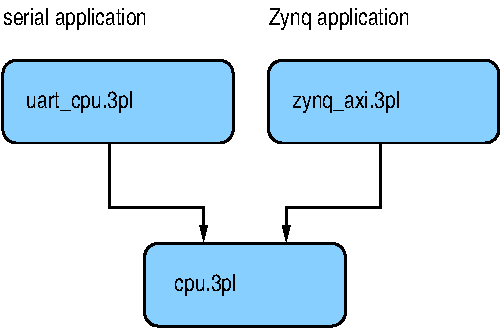
\includegraphics{cpu}
    
    Bus GP0 is used for reading 3PL expression values and queue mode variables
    and writing static and queue mode variables.

    Bus GP1 is used to read and write 3PL memory mode variables.

    For both GP buses burst transfers are used and burst lengths may be up to 8
    32-bit words. Burst transfers are executed in the CPU interface code by
    load/store multiple commands which use a contiguous set of registers. A
    maximum of 8 of the 16 available registers has been imposed, hence the
    maximum burst size of 8 32-bit words.

    An information file, design.info, is generated. This file lists the
    directives, AXI bus interface details and interrupt event parameters. The
    file is in JSON format. A python utility program, info2c,  extracts data
    from this information file and generates a .h file for CPU programs in C.
    Similar utilities may be written for other languages.

    info2c is a shell script invoking python. The first or only argument is the
    design name and info2c expects to find a file design.info. It will create a
    file design.h. If the optional second argument is provided then it is used
    as the output file name (".h" is appended).
    
    The design.info data may also be stored in block RAM (rmemory) for read-time
    access by CPU code. This is enabled by default but may be avoided via a
    directive, i.e. {\bf directive("excludeinfo", true);}, which can be executed
    at any time during 3PL immediate execution. The compression is done by
    calling inbuilt function {\bf deflate()} \autorefph{sec:ifdeflate}. The
    readback is initialised by writing to address 1 and 32-bit packed .info data
    is then read by successive 32-bit reads from address 1. The first read
    returns a 32 bit CRC-32 checksum for the remainder of the block,\. The
    second read returns the uncompressed data size in bytes and the third read
    returns the compressed data size in bytes. Reads beyond the data length will
    return zeros.
    
    The data block size depends on the size of the compressed .info data and
    varies from a minimum of 1024 32 bit words (1 RAM block) to 32,768 words (32
    RAM blocks).

    These bus interfaces allocate successive addresses. These addresses are
    embedded in C functions generated by info2c and hence the programmer does
    not need to know the addresses (they can be determined from the .info file).
    Each interface is supplied a unique name in the 3PL procedure call and this
    name is used in the associated generated function names.

    For 3PL int types info2c will generate matching C types int8\_t, int16\_t,
    int32\_t or int64\_t as appropriate to the size of the datum. The maximum
    primitive size is 64 bits.

    For 3PL uint or bits types info2c will generate matching C types uint8\_t,
    uint16\_t, uint32\_t or uint64\_t as appropriate to the size of the datum.
    The maximum primitive size is 64 bits.

    For 3PL log type info2c will generate matching type bool\_t

    For  3PL structs or enums info2c will generate a matching C bit field
    struct. The maximum size for a struct is 64 bits.

    For a 3PL float type info2c will generate a C float or double type if the
    the type matches IEEE 754 format, otherwise it will generate a C bit field
    struct containing the exponent and mantissa as fields.

    The 3PL data type may be an array of uint, bits or int of exactly 32 or 64
    bits where the dimension is a maximum of 8 for 32 bit members or 4 for 64
    bit members. The matching C type generated will be a struct containing the
    array.



    \subsection{library modules}


        \subsubsection{cpu\_write\_dma\_buffer - DMA transfer to CPU RAM}\label{sec:lmzynqdmabufr}

            {\bf Library: xilinx/zynq\_axi.3pl}

            {\bf Prototype:} \\
            \vsp
            \begin{lstlisting}[gobble=12, language=threepl]
               global module
               cpu_write_dma_buffer (
                   str(name),          // interface name
                   int(blockwords),    // block length in data words
                   int(nblocks),       // number of blocks
                   queue(in),          // data in
                   log(use_wcount),    // use queue count rather than interrupt
                   log(bigendian)      // transfer data as bigendian
               ) {}
            \end{lstlisting}

            {\bf Output parameters:} \\
            none

            {\bf Input parameters:} \\            
            {\bf name} is a string identifier for the interface.\\
            {\bf blockwords} is the DMA block length in data words.\\
            {\bf nblocks} is the number of DMA blocks used.\\
            {\bf in} is a queue of data to be transferred.\\
            {\bf use\_wcount} determines whether an interrupt or a count are
            to be used to determine when to read the 'done' queue.
            
            This module creates a DMA buffer management interface allowing the FPGA
            to write directly to CPU RAM using DMA. For a simpler interface see {\bf
            dma\_write()} \autorefph{sec:lmzynqwrdma}. The parameter {\bf name} is
            used when creating the interface functions for this module.
            
            The interface will use the next unused HP bus of the four available.
            If all four HP buses have been used then a fatal error is invoked.
            
            The interface has two queues accessible to the CPU, a 'free' queue and
            a 'done' queue.
            
            The 'free' queue contains block numbers that are available to the DMA
            for writing. This queue is loaded initially by the CPU. The DMA
            interface removes a block number from the 'free' queue when it is to
            begin writing a block. If this queue is empy then DMA will wait until
            a block number is written to it by the CPU.

            When the DMA has finished filling a block in CPU RAM then it writes
            the block number to a 'done' queue. The block numbers read from the
            'done' queue can be used to compute the associated buffer address in
            mapped DMA memory.
            
            If {\bf use\_wcount} has no argument or the argument value is FALSE
            then there is an interrupt associated with that queue on which the
            CPU can wait for completed blocks to be signalled. The interrupt is
            a level which can be used to control a loop reading one item from
            the queue on each iteration.
            
            If {\bf use\_wcount} has a TRUE argument then the number of block
            numbers queued in the done queue can be determined and read in
            a count-controlled loop.
            
            The CPU must return a block number read from the 'done' queue to the
            'free' queue after it has completed processing the data in the block.
            
            The status of block numbers in the range of blocks available for use
            is recorded in memory in this DMA interface. This status can be used
            when recovering from a CPU crash but not reloading the FPGA
            configuration. The status for a block can be read or written by the
            CPU and will be one of -

            \blist
            \item   missing - the block number is missing from the DMA interface.
            It presumably has been removed by the CPU and not yet returned.
            \item   free - the block is free for a DMA transfer
            \item   done - a DMA transfer has been completed for this block
            \item   busy - the block is currently being written by a DMA transfer
            \blend
                        
            The data input queue {\bf in} must be of type -

            \begin{lstlisting}[gobble=12, language=threepl]
               struct(...,
                   data,       ...user data type ...,
                   term,       dma_block_term,
                   tag,        tagtype
               );
            \end{lstlisting}

            where\\
            \blist
            \item {\bf data} is the user data which can be any type\\
            \item {\bf term} is a block termination enumerated type
            'dma\_block\_term' which is\\
                \blist
                \item {\bf 'none'} (default) to add the datum to the current block\\
                \item {\bf 'ignore'} to terminate the block, discarding the
                accompanying datum\\
                \item {\bf 'first'} to start a new block with the datum
                \item {\bf 'last'} to add the current datum to the block then
                terminate the block\\
                \blend
            \item {\bf tag} is a user-defined field which can be used to
            distinguish blocks of different content. The tag field of the last
            datum to be added to the current block is used as the block tag, all
            previous ones being ignored.
            \blend
            
            The block termination mechanism will not terminate an empty block.

            Blocks will be terminated when full if not explicitly terminated by use
            of the termination field.

            The input data type is rounded up in size to 8, 16, 32 or 64 bits,
            zero padded at the MSB end where necessary.
            Data are packed into 64-bit words for transmission across an HP bus
            to CPU memory. The packing is 8x8, 4x16, 2x32 or 1x64.
            Where a block is terminated before being filled any unfilled portion of
            the last 64-bit word will be zero. The remainder of the block in CPU
            memory remains unwritten.

            On completion of a block transfer the structure that is read by
            the CPU from the 'done' queue is -

            \begin{lstlisting}[gobble=12, language=threepl]
               struct(bnctype,
                  blocknum,    "uint:"+size(nblocks),
                  words,       "uint:"+size(blockwords),
                  tag,         tagtype
               );
            \end{lstlisting}

            where -
            \blist
            \item {\bf blocknum} is the block number in the DMA buffer space\\
            \item {\bf words} gives the number of words of packed user data in the block\\
            \item {\bf tag} is a user-defined block tag\\
            \blend
            
            The Zynq ARM processor is little-endian and this is the default transfer
            order. If the argument to parameter {\bf bigendian} is supplied and is
            true the data will be transferred in big-endian order instead. This
            might be used if the data is to be transferred unprocessed out of the
            Zynq to another processor which is big-endian.



            
            
            The following C functions will be created from the .info file and placed
            into an include file by executing the python script info2c -
            
            \begin{tabular}{| l | l | l |}
            \hline
            fpga\_{\em name}\_done\_read()                  &   & read done queue block number and word count\\ \hline
            fpga\_{\em name}\_done\_avail\_read()           & 1 & read number of words in done queue     \\ \hline
            fpga\_{\em name}\_done\_avail\_thresh\_write()  &   & set interrupt threshold for done queue \\ \hline
            fpga\_{\em name}\_done\_enable()                & 2 & enable done queue interrupt            \\ \hline
            fpga\_{\em name}\_done\_disable()               & 2 & disable done queue interrupt           \\ \hline 
            fpga\_{\em name}\_done\_wait()                  & 2 & wait on done queue interrupt           \\ \hline  
            fpga\_{\em name}\_free\_write()                 &   & write to free queue                    \\ \hline  
            fpga\_{\em name}\_status\_read()                &   & read block status memory              \\ \hline  
            \end{tabular}
            
            Notes:\\
            1 - only if argument wcount is true\\
            2 - only if argument wcount is omitted or false
            
            in addition entries similar to the following will also be placed
            in the include file -
            
            \begin{tabular}{| l |}
            \hline
            const unsigned fpga\_{\em name}\_blocks 4; \\
            const unsigned fpga\_{\em name}\_block\_size 160; \\
            const unsigned fpga\_{\em name}\_block\_words 80; \\
            const unsigned fpga\_{\em name}\_port 0; \\
            typedef uint32\_t fpga\_{\em name}\_t; \\
            \hline
            \end{tabular}

            In the following {\bf fpga} is the pointer to the FPGA
            structure returned by {\bf fpga\_open()}.
            
            {\bf fpga\_{\em name}\_done\_enable(fpga)}
            
            Enable the interrupt on the block completion queue non-empty. This is
            only available if {\bf use\_wcount} is FALSE.
            
            {\bf fpga\_{\em name}\_done\_wait(fpga, NULL)}
            
            Wait on the interrupt on the block completion queue. Execution will
            continue, and the interrupt is disabled, when the queue is not empty.
            This is only available if {\bf use\_wcount} is FALSE. The second
            argument if not NULL is a timeout period (struct timeval).
            
            {\bf fpga\_{\em name}\_done\_avail\_read(fpga)}
            
            Read the availability count on the block completion queue. This is
            only available if {\bf use\_wcount} is TRUE.
            
            {\bf fpga\_{\em name}\_done\_read(fpga)}
            
            Read the block completion queue. The function returns a structure
            similar to the following -
            
            \begin{lstlisting}[gobble=12, language=C]
               typedef union {
                   struct {
                       uint16_t blocknum: 3;
                       uint16_t words: 6;
                       uint16_t blocktype: 2;
                       uint16_t : 5;
                   };
                   uint16_t __word;
               } fpga_{\em name}_done_t;
            \end{lstlisting}
            where {\bf blocknum} is the
            block number of a completed block in the DMA buffer,
            {\bf words} is the number of words of type {\bf fpga\_{\em name}\_t}
            written to that buffer (i.e. data words, not necessarily 64-bit words)
            and {\bf blocktype} is the user's arbitrary block type code. The
            last unnamed field (5) is padding to make up 16 bits.
            
            {\bf fpga\_{\em name}\_free\_write(fpga, blocknum)}
            
            Write a block number to the free block queue for re-use by the
            DMA interface ({\bf blocknum} is just an integer, not the struct
            shown above).

            {\bf fpga\_{\em name}\_status\_read(fpga, blocknum)}
            
            Read the status of a block from the DMA interface.
            For an interface named "xyz" the returned status would be a
            byte of type -
            
            \begin{lstlisting}[gobble=12, language=C]
                typedef enum {
                    fpga_xyz_status_busy = 2,
                    fpga_xyz_status_done = 3,
                    fpga_xyz_status_free = 1,
                    fpga_xyz_status_missing = 0,
                } fpga_xyz_status_t;
            \end{lstlisting}
            
            Any block number that has status 'missing' can be written to the free
            queue to make it once again available for use.
            
            {\bf const unsigned fpga\_{\em name}\_blocks}
            
            The number of DMA blocks for this interface.
            
            {\bf const unsigned fpga\_{\em name}\_block\_size}
            
            The block length in bytes for this interface, rounded up to a
            multiple of 8.
            
            {\bf const unsigned fpga\_{\em name}\_block\_words}
            
            The number of data words in this block.

            {\bf const unsigned fpga\_{\em name}\_port}
            
            The HP bus used for this interface, 0 to 3.
            
            {\bf typedef uint32\_t fpga\_{\em name}\_t}
            
            The type of data word.
            
            The CPU C code (using interrupt) might appear as follows,
            "DMA1" being the interface name -
            
            \begin{lstlisting}[gobble=12, language=C]
                   fpga_t *        fpga = NULL;
                   fpga_DMA_done_t bn;

                   nrete( fpga = fpga_open(fpga_unit_default, fpga_flag_default) );
                   erete( fpga_configdata_load(fpga, prog_fpga_config_data, prog_fpga_config_size) );
                   erete( fpga_map (fpga) );
    
                   // Load the block numbers into the 'free' queue.
                   for (i=0 ; i<HP0_buffers ; i++)
                       fpga_DMA1_free_write(fpga, i);

                   fpga_DMA1_done_enable(fpga);                     // enable interrupt
                   for (;;) {
                       erete( fpga_DMA1_done_wait(fpga, NULL) );
                       // When there is a completed block number available
                       // read it, process the data in the associated buffer,
                       // then return the block number of the now free block.
                       bn = fpga_DMA1_done_read(fpga);             // fetch block number
                       p = fpga->dma.base + bn.blocknum * fpga_DMA1_block_size;
                       for (int i=0 ; i<bn.words ; i++) {
                           .
                           . process data in DMA buffer block pointed to by p
                           .
                       }
                       fpga_DMA1_free_write(fpga, bn.blocknum);    // return block number
                       fpga_DMA1_done_enable(fpga);                // re-enable interrupt
                   }
            \end{lstlisting}

            The code in this module executes in the bus clock domain (c100).
            The clock domain in use when this module is called is restored when
            the module is exited.




        \subsubsection{create\_bus\_interfaces - create the individual CPU interfaces}\label{sec:lmzynqdmabufr}

            {\bf Library: xilinx/zynq\_axi.3pl)}

            {\bf Prototype:} \\
            \vsp
            \begin{lstlisting}[gobble=12, language=threepl]
                module
                create_bus_interfaces () {}
            \end{lstlisting}
            
            {\bf Output parameters:} \\
            
                none.                       
            
            {\bf Input parameters:} \\
            
                none.
                       
            {\bf description:} \\
            This module creates the logic for each of the CPU interfaces. Each
            of these communicates via queues to logic within {\bf zynq\_ps()}
            \autorefph{sec:lpzynqps} below.




    
        \subsubsection{dma\_read - DMA transfer from memory to FPGA}\label{sec:lmzynqrddma}

            {\bf Library: xilinx/zynq\_axi.3pl}


            {\bf Prototype:} \\
            \vsp
            \begin{lstlisting}[gobble=12, language=threepl]
               global module
               dma_read (
                   queue(data, "bits:64")
                   <-
                   int(bus),
                   queue(address, "uint:32"),
                   queue(burstlen, "uint:4")
               ) {}
            \end{lstlisting}

            {\bf Output parameters:} \\Zynq
            {\bf data} is the memory data read

            {\bf Input parameters:} \\            
            {\bf bus} is the high performance master bus, 0 to 3 \\  
            {\bf address} is the physical memory address from which to read \\  
            {\bf burstlen} is the burst length, which is the number of data
            words to be read

            {\bf description:} \\            
            DMA from RAM to FPGA using an AXI HP bus.
            This is a low-level module, providing only a simple DMA interface.
            
            This module can also be called indirectly via library cpu.3pl
            as a procedure in class {\bf CPU\_API}.
            \autorefph{chap:lmxilcpulib} {\bf FPGA to CPU interface Library
            - xilinx/cpu.3pl}.
            
            A datum on each of queues 'address' and 'burstlen' will trigger the
            DMA transfer if queue 'data' is not full. The transfer will consume
            one datum from each of 'address' and 'burstlen' and will write the
            number of data to queue 'data' necessary to satisfy the burst length.
            changed by this procedure,

            The code in this module executes in the bus clock domain (c100).
            The clock domain in use when this module is called is restored when
            the module is exited.



    
        \subsubsection{dma\_write - DMA transfer from FPGA to memory}\label{sec:lmzynqwrdma}

            {\bf Library: xilinx/zynq\_axi.3pl}


            {\bf Prototype:} \\
            \vsp
            \begin{lstlisting}[gobble=12, language=threepl]
               global module
               dma_write (
                   <-
                   int(bus),
                   queue(data, "bits:64")
                   queue(address, "uint:32"),
                   queue(burstlen, "uint:4")
               ) {}
            \end{lstlisting}

            {\bf Output parameters:} \\
            {\bf data} is the memory data read

            {\bf Input parameters:} \\            
            {\bf bus} is the high performance master bus, 0 to 3 \\  
            {\bf address} is the physical memory address to write to \\  
            {\bf burstlen} is the burst length, which is the number of data
            words to be written minus 1

            {\bf description:} \\            
            DMA from PL to RAM using an AXI HP bus.
            This is a low-level module, providing only a simple DMA interface.
            See {\bf cpu\_write\_dma\_buffer()} \autorefph{sec:lmzynqdmabufr}
            for a higher level interface supporting CPU buffer control.
            This is a low-level module, providing only a simple DMA interface.            
            
            This module can also be called indirectly via library cpu.3pl
            as a procedure in class {\bf CPU\_API}.
            \autorefph{chap:lmxilcpulib} {\bf FPGA to CPU interface Library
            - xilinx/cpu.3pl}.
    
            A datum on each of queues 'address' and 'burstlen' will trigger the
            DMA transfer if queue 'data' is not empty. The transfer will consume
            one datum from each of 'address' and 'burstlen' and will read the
            number of data from queue 'data' necessary to satisfy the burst
            length. The 'burstlen' is from 0 for one word to 15 for 16 words.

            The code in this module executes in the bus clock domain (c100).
            The clock domain in use when this module is called is restored when
            the module is exited.

            not empty.

        \subsubsection{sigint - interrupt the CPU on a signal}\label{sec:lmzynqcpusigint}

            {\bf Library: xilinx/zynq\_axi.3pl)}

            {\bf Prototype:} \\
            \vsp
            \begin{lstlisting}[gobble=12, language=threepl]
                module
                sigint(int(n), value(sig, "log")) {}
            \end{lstlisting}
            
            {\bf Output parameters:} \\
            
                none.                       
            
            {\bf Input parameters:} \\
                        
                {\bf n} is the interrupt index, 0 to 16.\\
                {\bf sig} is a signal on whose rising edge the interrupt
                is triggered.\\
                       
            {\bf description:} \\
            When the signal {\bf sig} is asserted the interrupt is triggered.
            The interrupt number, 0 to 15, is given by {\bf index}.



    
        \subsubsection{zynq\_ps - instantiate Zynq CPU}\label{sec:lpzynqps}

            {\bf Library: xilinx/zynq\_axi.3pl}

            {\bf Prototype:} \\
            \vsp
            \begin{lstlisting}[gobble=12, language=threepl]
               module
               zynq_ps () {}
            \end{lstlisting}

            {\bf Output parameters:} \\
            none

            {\bf Input parameters:} \\            
            none
        
            {\bf In-line target execution:} \\
            no

            {\bf description:} \\            
            This instantiates the Zynq CPU and connects the DDR RAM and
            general purpose I/O pins to the CPU. It also defines all the
            CPU pins. After calling this module all the following
            procedures are available.

            The code in this module executes in the bus clock domain (c100).
            The clock domain in use when this module is called is restored when
            the module is exited.



    
    \subsection{library procedures}

                                           
            


        \subsubsection{add\_interface - add an interface to the interface list}\label{sec:lpzynqcpuai}

            {\bf Library: xilinx/zynq\_axi.3pl)}

            {\bf Prototype:} \\
            \vsp
            \begin{lstlisting}[gobble=12, language=threepl]
                procedure
                add_interface (var(v, "->")) {}
            \end{lstlisting}
            
            {\bf Output parameters:} \\
            
                none.
                       
            {\bf Input parameters:} \\
            {\bf v} is an instance of class {\bf busCommon}, defined in
            cpu.3pl.
                     
            {\bf description:} \\
            The instance of {\bf busCommon} is added to the interface list.
            The list is processed at completion of immediate execution to
            create the whole CPU interface.




        \subsubsection{cpu\_read - write to CPU}\label{sec:lpzynqcpurd}

            {\bf Library: xilinx/zynq\_axi.3pl)}

            {\bf Prototype:} \\
            \vsp
            \begin{lstlisting}[gobble=12, language=threepl]
                procedure
                cpu_read (
                    value(access, "log"),
                    value(init, "log"), 
                    queue(out)
                    <-
                    int(bus),
                    int(addr),
                    value(data_in),
                    value(contin, "log")
                ) {}
            \end{lstlisting}
            
            {\bf Output parameters:} \\
            {\bf access} is an optional output parameter which is asserted
            when a CPU to FPGA write occurs.\\
            {\bf init} is an output parameter which is asserted in the case
            of a memory read to initiate the read.\\
            {\bf out} is an optional queue variable which will be written to
            when a transfer occurs.\\

                       
            {\bf Input parameters:} \\
            {\bf bus} is not used (applies to Zynq).\\
            {\bf address} is a 6 bit interface address.\\
            {\bf data\_in} input data.\\
            {\bf contin} is only used for a memory read and is asserted
            when the memory read has occured and the transfer can begin.\\
                     
            {\bf description:} \\
            This procedure provides a low-level interface to transfer
            data from the FPGA to the CPU via the USB serial port. It is
            used by modules and procedures in library cpu.3pl and is not
            intended for use directly by application code.
            
            The CPU initiates the transfer. The transfer may consist of
            multiple bytes.


        \subsubsection{cpu\_write - write to CPU}\label{sec:lpzynqcpuwr}

            {\bf Library: xilinx/zynq\_axi.3pl)}

            {\bf Prototype:} \\
            \vsp
            \begin{lstlisting}[gobble=12, language=threepl]
                procedure
                cpu_write (
                    var(out),
                    value(access, "log")
                    <-
                    int(bus),
                    int(addr)
                ) {}
            \end{lstlisting}
            
            {\bf Output parameters:} \\
            {\bf var} is a static or queue mode variable.\\          
            {\bf access} is an optional output parameter which is asserted
            when a CPU to FPGA write occurs.\\
                       
            {\bf Input parameters:} \\
            {\bf bus} is not used (applies to Zynq).\\
            {\bf address} is a 6 bit interface address.\\           
                     
            {\bf description:} \\
            This procedure provides a low-level interface to transfer
            data from the CPU to the FPGA via the USB serial port. It is
            used by modules and procedures in library cpu.3pl and is not
            intended for use directly by application code.
            
            The CPU initiates the transfer. The transfer may consist of
            multiple bytes.





    \subsection{library functions}
            

        \subsubsection{cpu\_api - CPU communications interface}\label{sec:lfcpuapi}

            {\bf Library: xilinx/zynq\_axi.3pl)}

            {\bf Prototype:} \\
            \vsp
            \begin{lstlisting}[gobble=12, language=threepl]
               global function
               cpu_api () {}
            \end{lstlisting}

            {\bf Return mode and type:} \\
            immediate, class

            {\bf Input parameters:} \\            
            
            none.
            
            {\bf description:} \\
            This function returns an instance of class CPU\_API

            {\bf Library: xilinx/zynq\_axi.3pl}

            {\bf Prototype:} \\
            \vsp
            \begin{lstlisting}[gobble=12, language=threepl]
                global function cpu_api () {}
            \end{lstlisting}
    
        None.




    \subsection{library classes}
    
        None.




\pagebreak

\section{FPGA to CPU interface Library File - xilinx/cpu.3pl}
\label{chap:lmxilcpulib}

    \index{library!xilinx/cpu.3pl}
    This library provides a class for basic FPGA-CPU interface for platforms
    which provide a communications path between a CPU and FPGA. This includes
    the zynq FPGA and various FPGA prototype boards which have a USB port for
    configuration loading and serial data communications. These procedures allow
    the CPU to read and write static variables, queues and memories and the FPGA
    to interrupt the CPU.
    
    This library contains alternative interfaces for reading and writing 3PL
    variables from the CPU. There are class procedures which are mode-specific - \\
            \hspace*{1cm}{\bf CPU\_API.read\_value()}\\
            \hspace*{1cm}{\bf CPU\_API.read\_queue()}\\
            \hspace*{1cm}{\bf CPU\_API.read\_memory()}\\
            \hspace*{1cm}{\bf CPU\_API.write\_static()}\\
            \hspace*{1cm}{\bf CPU\_API.write\_queue()}\\
            \hspace*{1cm}{\bf CPU\_API.write\_memory()}\\
    and there are generic class procedures - \\
            \hspace*{1cm}{\bf CPU\_API.read()}  \\          
            \hspace*{1cm}{\bf CPU\_API.write()}\\
    
    The former have the advantage that the mode of the variable being accessed
    is reflected in the procedure identifer and this may improve the readability
    the source code. On the other hand the latter are generic and shorter.
    
    There are DMA class modules for reading and writing CPU memory from the
    FPGA -\\
            \hspace*{1cm}{\bf CPU\_API.dma\_read()} \\
            \hspace*{1cm}{\bf CPU\_API.dma\_write()}\\
    and an interrupt class module and an interrupt class procedure -\\
            \hspace*{1cm}{\bf CPU\_API.sigint()}\\
            \hspace*{1cm}{\bf CPU\_API.interrupt()}\\
            
    For example the following three examples are equivalent - 

    \begin{lstlisting}[gobble=12, language=threepl]
        cpu_api.read_queue(entries, , acc <- q, "QR", true, 10 );
    \end{lstlisting}

    \begin{lstlisting}[gobble=12, language=threepl]
        cpu_api.read_queue(entries, , acc <- q, "QR", wordcount=true, ilevel=10 );
    \end{lstlisting}

    \begin{lstlisting}[gobble=12, language=threepl]
        cpu_api.read(count=entries, access=acc <- q, "QR", wordcount=true, ilevel=10);
    \end{lstlisting}
    
    A more detailed description of use of this class can be found in
    (\autorefph{ch:serialcpu}) for platforms with a USB serial link to the
    FPGA and (\autorefph{ch:zynqcpu}) for Zynq platforms. These sections
    include both C and Python3 coding examples.
    
    
    This library is incorporated by using a {\bf source} statement -
    \begin{lstlisting}[gobble=4, language=threepl]
       source "xilinx/cpu.3pl"
    \end{lstlisting}
    {\bf however this library is already included via xilinx/uart\_cpu.3pl
    (\autorefph{chap:lmuartcpulib}) or xilinx/zynq\_axi.3pl
    (\autorefph{chap:lmzynqaxilib}) and so should not be included directly by
    application programs.}

    
    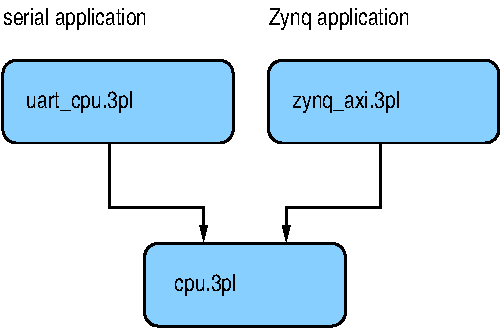
\includegraphics{cpu}

    
    xilinx/zynq\_axi.3pl is included in -\\
    boards/avnet/microzed\_7010.3pl\\
    boards/avnet/microzed\_7020.3pl\\
    boards/digilent/zybo.3pl
    
    xilinx/uart\_cpu.3pl is included in -\\
    boards/avnet/aes\_sp3a\_eval400.3pl\\
    board/gadget\_factory/papilio\_one\_100.3pl\\
    board/gadget\_factory/papilio\_one\_250.3pl\\
    board/gadget\_factory/papilio\_one\_500.3pl\\
    board/gadget\_factory/papilio\_pro\_lx4.3pl\\
    board/gadget\_factory/papilio\_pro\_lx9.3pl
    
    The class for the FPGA interface is created by -
    
    \begin{lstlisting}[gobble=4, language=threepl]
    class(cpu, CPU_API());
    \end{lstlisting}

    cpu.3pl -
    \blist   
    \item   defines class {\bf busCommon} which is used to describe each
            interface.    
    \item   creates an instance of class {\bf CPU\_CODEGEN} whose procedures
            create the logic to implement each type of interface.        
    \item   creates an instance of class {\bf CPU\_API} whose modules
            provide the application program interface. Procedures within
            this class create instances of {\bf busCommon} and add them to
            an interface list. {\bf busCommon} contains all the information
            necessary to create a CPU interface. Class {\bf CPU\_API} in
            turn assigns module create\_bus\_interfaces() as a trailer
            module.
    \blend
    
    Module create\_bus\_interfaces() executes at the end of immediate execution
    (it is a trailer module). It creates the basic CPU interface logic by
    calling module {\bf cpu\_interface} and then traverses the interface list
    and creates code for each interface via procedures in class {\bf
    CPU\_CODEGEN}.
    
    {\bf CPU\_API}, {\bf CPU\_CODEGEN}, {\bf create\_bus\_interfaces} and
    {\bf cpu\_interface} are defined in both UART\_CPU.3pl and zynq\_axi.3pl,
    as the underlying interface logic is quite different for the two platforms.






    \subsection{class library modules}
            
                
        \subsubsection{CPU\_API.signal\_interrupt - interrupt from a signal}\label{sec:lpcpusigint}

            {\bf Library: xilinx/cpu.3pl}

            {\bf Prototype:} \\
            \vsp
            \begin{lstlisting}[gobble=12, language=threepl]

                module
                signal_interrupt (str(event), value(sig, "log")) {}
            \end{lstlisting}

            {\bf Output parameters:} \\
            
            none.

            {\bf Input parameters:} \\
            {\bf event} is the event identifier string.\\
            {\bf sig} is the signal causing the event.\\
        
            {\bf In-line target execution:} \\
            no

            {\bf description:} \\
            This procedure generates a module which will cause a CPU interrupt
            when its input signal {\bf sig} is asserted.
            The argument to parameter {\bf event} is an identifier with
            which to refer to the interrupt in the CPU interface software.

            See also class procedure {\bf interrupt()}
            \autorefph{sec:lpcpuint} which generates a CPU interrupt when
            executed in the FPGA.
    
     
     
     
     
        \subsubsection{CPU\_API.dma\_read - DMA transfer to FPGA from CPU}\label{sec:lpcpudmar}

            {\bf Library: xilinx/cpu.3pl}

            {\bf Prototype:} \\
            \vsp
            \begin{lstlisting}[gobble=12, language=threepl]
                module
                dma_read (
                    queue(data, "bits:64")      // read data
                    <-
                    queue(address, "uint:32"),  // memory address
                    queue(burstlen, "uint:4"),  // burst length - 1
                    int(bus)                    // HP bus 0 to 3
                ) {}
            \end{lstlisting}

            {\bf Output parameters:} \\
            
            {\bf data} is the queue to which data from the transfer is returned.\\

            {\bf Input parameters:} \\
            {\bf address} is a queue supplying the CPU memory physical read address.\\
            {\bf burstlen} is a queue giving the burst length in the case of Zynq.\\
            {\bf bus} is the HP bus, 0 to 3, in the case of Zynq.\\
        
            {\bf In-line target execution:} \\
            no

            {\bf description:} \\
            This procedure generates a module which reads data from the CPU
            memory. For platforms with serial communications between the
            FPGA and the CPU this is not really DMA but instead data is transferred
            from CPU memory by a software thread.
            
            In the case of a platform with a serial interface only one input
            argument, {\bf address}, is valid - {\bf burstlen} and {\bf bus} must
            not be given arguments. \bf{This address is relative to a base address
            set by calling} {\bf set\_dma\_address()} \autorefph{tools_c_serial}.
            
            When an address becomes available on the {\bf address} input queue
            and the output {\bf data} queue is not full a DMA transfer (read)
            will take place. For a serial interface platform this is not a real
            DMA transfer but is carried out in software by a separate CPU
            thread.

            For the Zynq the address is a physical address. When an address and
            a burstlength become available on the {\bf address} and {\bf
            burstlen} input queues and the output {\bf data} queue is not full,
            a DMA transfer (read) will take place. The HP bus selected cannot be
            used for any other interfaces.

            See also class module {\bf CPU\_API.dma\_write()}
            \autorefph{sec:lpcpudmaw} which generates a DMA write module.



        \subsubsection{CPU\_API.dma\_write - DMA transfer from FPGA to CPU}\label{sec:lpcpudmaw}

            {\bf Library: xilinx/cpu.3pl}

            {\bf Prototype:} \\
            \vsp
            \begin{lstlisting}[gobble=12, language=threepl]
                module
                dma_write (
                    queue(data, "bits:64"),     // write data
                    queue(address, "uint:32"),  // memory address
                    queue(burstlen, "uint:4"),  // burst length - 1
                    int(bus)                    // HP bus 0 to 3
                ) {}
            \end{lstlisting}

            {\bf Output parameters:} \\
            
            None.

            {\bf Input parameters:} \\
            {\bf data} is a queue supplying data for the transfer.\\
            {\bf address} is a queue supplying the CPU memory physical write address.\\
            {\bf burstlen} is a queue giving the burst length in the case of Zynq.\\
            {\bf bus} is the HP bus, 0 to 3, in the case of Zynq.\\
        
            {\bf In-line target execution:} \\
            no

            {\bf description:} \\
            This procedure generates a module which writes data to the CPU
            memory. For platforms with serial communications between the
            FPGA and the CPU this is not really DMA but instead data is transferred
            to CPU memory by a software thread.
            
            In the case of a platform with a serial interface only two input
            arguments, {\bf data} and {\bf address}, are valid - {\bf burstlen}
            and {\bf bus} must not be given arguments. \bf{This address is
            relative to a base address set by calling} {\bf set\_dma\_address()}
            \autorefph{tools_c_serial}.
            
            When data and an address become available on the {\bf data} and {\bf
            address} input queues a DMA transfer (read) will take place. For a
            serial interface platform this is not a real DMA transfer but is
            carried out in software by a separate CPU thread.

            For the Zynq When data, an address and a burstlength become available
            on the {\bf data}, {\bf address} and {\bf burstlen} input queues a
            DMA transfer (write) will take place. The HP bus selected cannot be
            used for any other interfaces.

            See also class module {\bf CPU\_API.dma\_read()}
            \autorefph{sec:lpcpudmar} which generates a DMA read module.



    
    \subsection{class library procedures}
            
                
        \subsubsection{CPU\_API.interrupt - interrupt procedure}\label{sec:lpcpuint}

            {\bf Library: xilinx/cpu.3pl}

            {\bf Prototype:} \\
            \vsp
            \begin{lstlisting}[gobble=12, language=threepl]

                procedure
                interrupt (str(event)) {}
            \end{lstlisting}

            {\bf Output parameters:} \\
            
            none.

            {\bf Input parameters:} \\
            {\bf event} is the event identifier string.\\
        
            {\bf In-line target execution:} \\
            yes

            {\bf description:} \\
            This procedure generates an interrupt when executed in the FPGA.
            The argument to parameter {\bf event} is an identifier with
            which to refer to the interrupt in the CPU interface software.

            See also class module {\bf signal\_interrupt()}
            \autorefph{sec:lpcpusigint} which creates a module which sources an
            interrupt from a signal.





        \subsubsection{CPU\_API.read - a CPU-readable interface}\label{sec:lpcpuread}

            {\bf Library: xilinx/cpu.3pl}

            {\bf Prototype:} \\
            \vsp
            \begin{lstlisting}[gobble=12, language=threepl]
                procedure
                read (
                        static(access, "log"),
                        varargs
                        <- 
                        str(name),
                        var(in),
                        varargs
                    ) {}
            \end{lstlisting}

            {\bf Output parameters:} \\
            {\bf access} is an optional static logical variable which is true
            for one clock cycle following a CPU read.
            {\bf varargs} optional output, parameters {\bf out} and {\bf count}.\\

            {\bf Input parameters:} \\
            {\bf in} is the value, queue, cmemory or rmemory mode variable
            to be read.\\
            {\bf name} is a string identifier for the interface.\\
            {\bf varargs} optional input parameters {\bf wordcount}, {\bf ilevel} and
                {\bf port}.\\
        
            {\bf In-line target execution:} \\
            no

            {\bf description:} \\
            This procedure creates a module which provides a CPU-readable
            interface for the the CPU for  3PL variables of mode value, static,
            queue, cmemory or rmemory.
            
            In the case of Zynq the interface uses AXI bus GP0.            
            The size of the input data type must not exceed 256 bits as the CPU
            interface software limits burst transfers to 8 32-bit words.
            
            Boards having a serial interface to the CPU use that interface.
            The size of the input data type must not exceed 1016 bits (127 bytes).
            
            The module is created at the end of immediate execution from
            arguments queued by this procedure. It can be any type, primitive or
            compound.
                        
            It is a common wrapper for the procedures \\
            {\bf CPU\_API.read\_value()} \autorefph{sec:lpcpurdvalue} \\
            {\bf CPU\_API.read\_queue()} \autorefph{sec:lpcpurdqueue} \\
            {\bf CPU\_API.read\_memory()} \autorefph{sec:lpcpurdmem} \\
            
            Parameter {\bf name} is a string identifier that can be used
            in the CPU code to refer to this interface.
            
            Parameter {\bf in} is the input variable or expression to be read
            by the CPU.
           
            Optional input and output varargs parameters are -
            
            \begin{tabular}{| l | l | l |}
            \hline
                    & input varargs         & output varargs    \\
            \hline \hline
            value   &                       &                   \\
            static  &                       &                   \\
            \hline
            queue   &   wordcount ilevel    & out count         \\
            \hline
            cmemory & port                  &                   \\
            rmemory &                       &                   \\
            \hline
            \end{tabular}




            
            \vspace{\baselineskip}\vspace{\baselineskip}
            {\Large \bfseries Value or Static mode}

                
                            Parameter {\bf in} is the value-mode input variable or expression.
            Since it is value mode the argument may be a value mode variable,
            static mode variable or an expression containing these. An expression
            must not contain a queue read.            
            
            The module is created at the end of immediate execution from arguments
            queued by this procedure. It can be any type, primitive or compound. The
            optional output static logical variable {\bf access} goes true for one
            clock cycle to indicate that a read has occurred.
            
            This procedure can be called via the more cryptic and general
            procedure {\bf cpu\_api.read()} \autorefph{sec:lpcpuread} instead.
            
            In the case of Zynq the interface uses AXI bus GP0.            
            The size of the input data type must not exceed 256 bits as the CPU
            interface software limits burst transfers to 8 32-bit words.
            
            Boards having a serial interface to the CPU use that interface.
            The size of the input data type must not exceed 1016 bits (127 bytes).
            

            The optional output static logical variable {\bf access} goes true
            for one clock cycle to indicate that a read has occurred.
            
            The clock domain of output {\bf access} need not be the same as
            that of {\bf in}. If {\bf access} has no clock domain it will be
            given the bus clock domain.
            
            The parameters associated with this bus interface, including an
            allocated bus address, are written
            to the {\em design}.info file.

            The utility info2c is used to process this file and create
            an include file {\em design}.h which contains a funcion
            definition to access this interface. for example the 3PL
            code
            \begin{lstlisting}[gobble=12, language=threepl]
               cpu_read_value("alpha", v);
            \end{lstlisting}
            will result in info2c producing a declaration like
            \begin{lstlisting}[gobble=12, language=C]
               uint32_t alpha_read (fpga_t * fpga) {}
            \end{lstlisting}
            
            When the CPU reads a value it is sampling that value, hence data may
            be lost if the sampling rate is lower than the rate at which data
            changes. The data sampling logic ensures that the data is a valid
            sample even when the source is changing at the time of the
            read. This is a primitive interface which depends on additional
            protocols being imposed by the application code. For example to
            guarantee data integrity a write to register the data in a static
            variable prior to reading could be used. For a more complex interface see {\bf cpu\_api.read\_queue()}
            \autorefph{sec:lpcpurdqueue}.
            
            On running info2c on the .json file the following C function will have been
            defined for interface {\em name} -
            
            \begin{tabular}{| l | l |}
            \hline
            function                   &                 \\ \hline \hline
            fpga\_{\em name}\_read()   & read a datum    \\ \hline
            \end{tabular}
            
            Example: \\
            If 3PL source file prog.3pl contains the following \\
            \begin{lstlisting}[gobble=12, language=threepl]
               class(cpu, cpu_api());
               
               static(s, "uint:16");
               .
               .
               cpu.read_value("S1", s);
               .
               .
            \end{lstlisting}
            the CPU code should contain something like \\
            \begin{lstlisting}[gobble=12, language=C]
                   #include "prog_fpga.h"
                   .
                   .
                   fpga_t *fpga = NULL;
                   int     d;
                   .
                   .
                   fpga_open(portName);
                   .
                   .
                   d = fpga_S1_read(fpga);
                   .
            \end{lstlisting}
            
            This procedure creates no in-line target code so the current clock domain
            when this procedure is called is not relevant. The clock domain is not
            changed by this procedure,
            The CPU code in Python3 should contain something like \\
            \begin{lstlisting}[gobble=12, language=python]
                import sys
                sys.path.append("/Users/......./install/3pl")
                import info2py
                import prog_fpga as fpga

                fpga_open()

                fpga = info2py.info_from_file("prog")   # load info from prog.info file

                d = fpga.P1_read()

            \end{lstlisting}

                        


            \vspace{\baselineskip}\vspace{\baselineskip}
            {\Large \bfseries Queue mode}
                        


                            Parameter {\bf in} is the queue-mode input variable.
            
            The queue must be written somewhere in the program (queues without
            sources result in a fatal error on completion of immediate
            execution). When the module is created the argument queue must have
            an established write clock domain or a fatal error is generated.

            If the input queue is read anywhere else in the program (i.e. other
            than in this module) then it must be read in the bus clock domain
            since that is the clock domain in which it is read in the module
            created by this procedure.

            If optional parameter {\bf wordcount} has an argument and it
            is true, the number of words in the queue buffer can be interrogated
            by the CPU. The input queue may have any of the allowed buffer sizes.
            If the queue is asynchronous, i.e. the read domain is not the bus
            clock domain, the count will not be exact but will be a guaranteed
            minimum number of readable data.

            If optional parameter {\bf wordcount} has an argument and it
            is false, the data returned from reading the number of words in the
            buffer is 0 or 1 instead of a count. A return of 1 means the queue
            buffer is not empty, i.e. can be read. This option is provided to
            simplify the logic where a simple empty/non-empty status is required.

            If optional parameter {\bf wordcount} has no argument then
            there will no interface to directly read the number of words in the
            queue buffer, however an interrupt may be used instead.            

            Note that an empty queue is guaranteed to return all ones to the CPU
            when read. For most data types this single value will usually be
            invalid and hence in that case it can be used as an indication of an
            empty queue. This can be used instead of explicitly reading the
            available word count.

            If an argument to optional parameter {\bf ilevel} is provided then a
            level interrupt on queue buffer status is established as follows -

            If there is no argument then no interrupt is provided.

            If the argument is type "log" with value false then the interrupt will
            be asserted when the queue buffer is not empty.

            If the argument is type "log" with value true then the interrupt will be
            asserted when the number of words in the buffer equals or exceeds a
            level which has been written to the interface from the CPU. The initial
            value of this level is 1. A level value of 0 should not be written to
            the interface as that will result in a continuous level interrupt
            regardless of queue state.

            If the argument is type "uint" or "int" then the interrupt will be
            asserted when the number of words in the buffer equals or exceeds the
            fixed value specified by the integer argument.

            The optional output parameter {\bf count} provides a count of the
            number of data in the queue. The inbuilt function queuewords() can
            only be used in a module which reads the queue, which is usually not
            the case where {\bf cpu\_api.read\_queue()} is the queue destination.
            {\bf count} must have clock domain {\bf bus\_clk}. If it has no clock
            domain, {\bf cpu\_api.read\_queue()} will set it to {\bf bus\_clk}.
            The width of {\bf count} must be sufficient to hold the input queue
            depth.

            If optional output parameter {\bf out} has an argument, each datum
            read from the input queue {\bf in} to the CPU local bus is also
            written to queue {\bf out}. The type of {\bf out} must be such that
            it can be assigned from {\bf in}. {\bf out} should not be allowed to
            block since it cannot stop data being popped from {\bf in} to the CPU
            bus. While {\bf out} in unavailable for writing, no attempt is made
            to write data popped from {\bf in} to it.

            If optional output parameter {\bf access} has an argument, the static
            variable of type "log" is assigned true for one clock cycle every
            time a datum is popped from the input queue {\bf in}. {\bf access}
            may have any clock domain.
            
            On running info2c on the .json file the following C functions will have
            been defined for interface {\em name} -
            
            \begin{tabular}{| l | l | l |}
            \hline
            function                                 & action when?           &                         \\ \hline \hline
            fpga\_{\em name}\_read()                 & always                 & read a datum            \\ \hline
            fpga\_{\em name}\_avail\_read()          & wordcount has argument & read number of words    \\ \hline
            fpga\_{\em name}\_avail\_thresh\_write() & ilevel "log" true      & set interrupt threshold \\ \hline
            fpga\_{\em name}\_enable()               & ilevel has argument    & enable interrupt        \\ \hline
            fpga\_{\em name}\_disable()              & ilevel has argument    & disable interrupt       \\ \hline 
            fpga\_{\em name}\_wait()                 & ilevel has argument    & wait on interrupt       \\ \hline  
            \end{tabular}
            
            Example: \\
            If 3PL source file prog.3pl contains the following \\
            \begin{lstlisting}[gobble=12, language=threepl]
                class(cpu, cpu_api());
                
                queue(p, "uint:16");
                .
                .
                cpu.read("P1", p, wordcount=false, ilevel=false);
                .
                .
            \end{lstlisting}
            the CPU code in C should contain something like \\
            \begin{lstlisting}[gobble=12, language=C]
                #include "prog_fpga.h"
                .
                .
                fpga_t *fpga = NULL;
                int     d[...];
                int     i = 0;
                .
                .
                fpga_open();
                .
                .
                fpga_P1_event_wait(fpga);
                while (fpga_P1_avail_read(fpga) != 0)
                    d[i++] = fpga_P1_read(fpga);
                .
            \end{lstlisting}
            The code will wait until the queue p goes from empty to non-empty
            when an interrupt will release the wait. A loop while the queue
            remains non-empty reads until the queue is empty. Note that since
            {\bf wordcount} is given an argument but the value is false, the count
            will only have values 0/1 for empty/not-empty.
           
            This procedure creates no in-line target code so the current clock
            domain when this procedure is called is not relevant. The clock domain
            is not changed by this procedure,
            
            The CPU code in Python3 should contain something like \\
            \begin{lstlisting}[gobble=12, language=python]
                import sys
                sys.path.append("/Users/......./install/3pl")
                import info2py
                from cpu_serial import *

                fpga_open()

                fpga = info2py.info_from_file("prog")   # load info from prog.info file

                d = []
                fpga.P1_wait()
                while (fpga.P1_avail_read() != 0)
                    d.append = fpga.P1_read()

            \end{lstlisting}
            
            Note that in the unusual case where a queue variable is both read and
            written by the CPU and is not otherwise accessed in the FPGA the input
            and output clock domains of the queue will be undefined. To overcome
            this the clock domain can be set when the queu is created, e.g.
            
            \begin{lstlisting}[gobble=12, language=threepl]
            queue(q, "uint10", domain=null);
            \end{lstlisting}
            
            which will set both the input (write) and output (read) clock domains
            to the current clock domain - see \autorefph{sec:ipqueue}).

                        


            
            \vspace{\baselineskip}\vspace{\baselineskip}
            {\Large \bfseries cmemory or rmemory mode}
            
                        
                            Parameter {\bf in} is the cmemory-mode or rmemory-mode input variable.
            
            If optional output parameter {\bf access} has an argument, the
            static variable of type "log" is assigned true for one clock cycle
            every time the port of {\bf in} is read. {\bf access} may have any
            clock domain.
            
            In the case of Zynq the interface uses AXI bus GP0.            
            The size of the input data type must not exceed 256 bits as the CPU
            interface software limits burst transfers to 8 32-bit words.
            
            Boards having a serial interface to the CPU use that interface.
            The size of the input data type must not exceed 1016 bits (127 bytes).
            
            This interface can use any memory port and that port can also be
            used by other application code, but no arbitration of shared access
            via a port is provided. Coincident access will usually result in
            data corruption. If it is not feasible to dedicate a port to CPU
            access then the CPU application code must limit acccess to the
            memory to times when it is known that the FPGA logic will not also
            be accessing the memory port.
            
            On running info2c on the .json file the following C function will have been
            defined for interface {\em name} -
            
            \begin{tabular}{| l | l |}
            \hline
            function                 &                                \\ \hline \hline
            fpga\_{\em name}\_read() & read a datum from FPGA memory  \\ \hline
            \end{tabular}
            
            Example: \\
            If 3PL source file prog.3pl contains the following \\
            \begin{lstlisting}[gobble=12, language=threepl]
               class(cpu, cpu_api());
               rmemory(m, 2, "uint:8", "uint:16");
               .
               .
               cpu.read_memory("MEM1", m, 0);
               .
               .
            \end{lstlisting}
            then for zynq the CPU code should contain something like \\
            \begin{lstlisting}[gobble=12, language=C]
                   #include "prog.h"
                   .
                   .
                   fpga_t *fpga = NULL;
                   int     d;
                   .
                   .
                   fpga_open();
                   .
                   .
                   d = fpga_MEM1_read(addr);
                   .
            \end{lstlisting}
            where addr is the memory address. The returned data is assigned
            to variable {\bf d}.

            This procedure creates no in-line target code so the current clock domain
            when this procedure is called is not relevant. The clock domain is not
            changed by this procedure,

            








        \subsubsection{CPU\_API.write - a CPU-writable interface}\label{sec:lpcpuwrite}

            {\bf Library: xilinx/cpu.3pl}

            {\bf Prototype:} \\
            \vsp
            \begin{lstlisting}[gobble=12, language=threepl]
                procedure
                write (
                        var(out),
                        varargs
                        <- 
                        str(name),
                        varargs
                    ) {
            \end{lstlisting}

            {\bf Output parameters:} \\
            {\bf out} is the target variable to be written to \\
            {\bf varargs} optional output parameter {\bf access} \\

            {\bf Input parameters:} \\
            {\bf name} is a string identifier for the interface.\\
            {\bf varargs} optional input parameters {\bf freecount}, {\bf ilevel}, {\bf port}
            and {\bf reset}.\\
        
            {\bf In-line target execution:} \\
            no

            {\bf description:} \\
            This procedure provides a write interface for the the CPU for 
            3PL variables of mode static, queue, cmemory or rmemory.
            
            In the case of Zynq the interface uses AXI bus GP0.            
            The size of the input data type must not exceed 256 bits as the CPU
            interface software limits burst transfers to 8 32-bit words.
            
            Boards having a serial interface to the CPU use that interface.
            The size of the input data type must not exceed 1016 bits (127 bytes).
            
            The module is created at the end of immediate execution from
            arguments queued by this procedure. It can be any type, primitive or
            compound.
                        
            It is a common wrapper for the procedures \\
            {\bf CPU\_API.write\_static()} \autorefph{sec:lpcpuwrstat} \\
            {\bf CPU\_API.write\_queue()} \autorefph{sec:lpcpuwrqueue} \\
            {\bf CPU\_API.write\_memory()} \autorefph{sec:lpcpuwrmem} \\
            
            Parameter {\bf name} is a string identifier that can be used
            in the CPU code to refer to this interface.
            
            Parameter {\bf out} is the output variable to be written to
            by the CPU.

            The only optional output parameter is {\bf access} which must have
            a static mode argument of type "log". If this optional parameter is
            given an argument then parameter {\bf out} may be omitted. In that
            case the write serves only to generate a single cycle pulse to
            the {\bf access} argument in the FPGA.
           
            Optional input varargs parameters are -
            
            \begin{tabular}{| l | l |}
            \hline
                    & input varargs             \\
            \hline \hline
            static  &                           \\
            \hline
            queue   & freecount ilevel reset    \\
            \hline
            cmemory & port                      \\
            rmemory &                           \\
            \hline
            \end{tabular}





            
            \vspace{\baselineskip}\vspace{\baselineskip}
            {\Large \bfseries Static mode}

                        
                            Parameter {\bf out} is the static-mode output variable. Its argument
            may be omitted if the optional parameter {\bf access} is given an argument.
            
            In the case of Zynq the interface uses AXI bus GP0.            
            The size of the output data type must not exceed 256 bits as the CPU
            interface software limits burst transfers to 8 32-bit words.
            
            Boards having a serial interface to the CPU use that interface.
            The size of the output data type is not limited.

            Output parameter {\bf out} is examined in order to determine its clock
            domain. If it has no clock domain it is given the bus clock domain.

            On running info2c on the .json file the following C function will
            have been defined for interface {\em name} -
            
            \begin{tabular}{| l | l |}
            \hline
            function                   & action         \\ \hline \hline
            fpga\_{\em name}\_write()  & write a datum  \\ \hline
            \end{tabular}
            
            Example: \\
            If 3PL source file prog.3pl contains the following \\
            \begin{lstlisting}[gobble=12, language=threepl]
               class(cpu, cpu_api());
               
               static(s, "uint:16");
               .
               .
               cpu.write_static(s <- "S2");
               .
               .
            \end{lstlisting}
            then for zynq the CPU code should contain something like \\
            \begin{lstlisting}[gobble=12, language=C]
                   #include "prog_fpga.h"
                   .
                   .
                   int     d;
                   .
                   .
                   fpga_open();
                   .
                   .
                   fpga_S2_write(d);          // write
                   .
            \end{lstlisting}

            This procedure creates no in-line target code so the current clock domain
            when this procedure is called is not relevant. The clock domain is not
            changed by this procedure,


                        
            

            \vspace{\baselineskip}\vspace{\baselineskip}
            {\Large \bfseries Queue mode}
                        


                            In the case of Zynq the interface uses AXI bus GP0.            
            The size of the output data type must not exceed 256 bits as the CPU
            interface software limits burst transfers to 8 32-bit words.
            
            Boards having a serial interface to the CPU use that interface.
            The size of the output data type is not limited.

            The queue must be read somewhere in the program (queues without
            sinks result in a fatal error on completion of immediate execution).
            When the module is created the argument queue must have an established
            read clock domain or a fatal error is generated.

            If the output queue is written anywhere else in the program (i.e. other
            than in this module) then it must be written in the bus clock domain
            (c100) since that is the clock domain in which it is written in this
            module.

            If the argument to {\bf freecount} is true the number of free entries in
            the queue buffer can be interrogated by the CPU. The output queue may
            have any of the allowed buffer sizes. If the queue is asynchronous, i.e.
            the write domain is not the bus clock domain (c100), the count will not
            be exact but will be a guaranteed minimum number of writable spaces.

            If the argument to {\bf freecount} is false the data returned from
            reading the number of free spaces in the buffer is 0 or 1 instead of a
            count. A return of 1 means the queue buffer is not full, i.e. can be
            written. This option is provided to simplify the logic where a simple
            full/non-full status is required.

            If {\bf freecount} has no argument then there will no interface to
            directly read the space remaining in the queue buffer, however an
            interrupt may be used instead.            

            Arguments to parameter {\bf ilevel} control provision of a level
            interrupt on queue buffer status as follows -

            If there is no argument then no interrupt is provided.

            If the argument is type "log" with value false then the interrupt will
            be asserted when the queue buffer is not full.

            If the argument is type "log" with value true then the interrupt will be
            asserted when the number of free spaces in the buffer equals or exceeds
            a level which has been written to the interface from the CPU. The
            initial value of this level is 1. A level value of 0 should not be
            written to the interface as that will result in a continuous level
            interrupt regardless of queue state.

            If the argument is type "uint" or "int" then the interrupt will be
            asserted when the number of free spaces in the buffer equals or exceeds
            the fixed value specified by the integer argument. Again this should not
            be 0.

            If parameter {\bf reset} has an argument it provides a means of
            resetting (clearing) the output queue. The argument may have a
            different clock domain to that of the write side of the queue and hence
            this may be more convenient than directly resetting the queue where a
            change of clock domain may need to be explicitly provided.

            Note that a write to a queue variable from {\bf cpu\_api.write\_queue()} (or
            indeed from anywhere) can be detected within the FPGA by means of the
            inbuilt function {\bf waswritten()} \autorefph{sec:ifwaswritten}. When
            using this function the clock domain must be the same as that of the
            queue write, i.e. {\bf bus\_clk}.
            Parameter {\bf out} is the queue-mode output variable.
            
            On running info2c on the .json file the following C functions will have
            been defined for interface {\em name} -
            
            \begin{tabular}{| l | l | l |}
            \hline
            function                                 & when                   &                            \\ \hline \hline
            fpga\_{\em name}\_write()                & always                 & write a datum              \\ \hline
            fpga\_{\em name}\_avail\_read()          & freecount has argument & read number of spaces free \\ \hline
            fpga\_{\em name}\_avail\_thresh\_write() & ilevel "log" true      & set interrupt threshold    \\ \hline
            fpga\_{\em name}\_enable()               & ilevel has argument    & enable interrupt           \\ \hline
            fpga\_{\em name}\_disable()              & ilevel has argument    & disable interrupt          \\ \hline 
            fpga\_{\em name}\_wait()                 & ilevel has argument    & wait on interrupt          \\ \hline  
            \end{tabular}


            
            Example: \\
            If 3PL source file prog.3pl contains the following \\
            \begin{lstlisting}[gobble=12, language=threepl]
               class(cpu, cpu_api());
               queue(p, "uint:16");
               .
               .
               cpu.write_queue(p <- "P2",, true);
               .
               .
            \end{lstlisting}
            then for zynq the CPU code should contain something like \\
            \begin{lstlisting}[gobble=12, language=C]
                   #include "prog_fpga.h"
                   .
                   .
                   fpga_t *fpga = NULL;
                   int     d[...];
                   int     i = 0;
                   int     n = sizeof(d) / sizeof int;
                   .
                   .
                   fpga_open(portName, INTERRUPTS);
                   .
                   .
                   fpga_P2_avail_thresh_write(fpga, n); // set interrupt level
                   fpga_P2_wait(fpga);                  // wait for interrupt
                   for (i=0 ; i<n ; i++) {              // transmit data block
                       fpga_P2_write(fpga, d[i]);       // write item
                   fpga_P2_enable(fpga);                // enable interrupt
                   .
            \end{lstlisting}
            
            or perhaps -
            \begin{lstlisting}[gobble=12, language=threepl]
               class(cpu, cpu_api());
               queue(p, "uint:16");
               .
               .
               cpu.write_queue(p <- "P2", false);
               .
               .
            \end{lstlisting}
            then for zynq the CPU code should contain something like \\
            \begin{lstlisting}[gobble=12, language=C]
                   #include "prog_fpga.h"
                   .
                   .
                   fpga_t *fpga = NULL;
                   int     d[...];
                   int     i = 0;
                   int     n = sizeof(d) / sizeof int;
                   .
                   .
                   fpga_open(portName, INTERRUPTS);
                   .
                   .
                   for ( i=0 ; i<n ; i++) {                // transmit data block
                       while (fpga_P2_avail(fpga) == 0)    // poll until not full
                           ;
                       fpga_P2_write(fpga, d[i]);          // write item
                   }
                   .
            \end{lstlisting}

            This procedure creates no in-line target code so the current clock domain
            when this procedure is called is not relevant. The clock domain is not
            changed by this procedure,
            
            {\bf The support CPU software for the UART CPU interface is still
            under development, but application code wil be similar to the
            above.}

                        
            

            
            \vspace{\baselineskip}\vspace{\baselineskip}
            {\Large \bfseries cmemory or rmemory mode}
            
                            Parameter {\bf out} is the cmemory or rmemory mode output variable.

            
            In the case of Zynq the interface uses AXI bus GP0.            
            The size of the output data type must not exceed 256 bits as the CPU
            interface software limits burst transfers to 8 32-bit words.
            
            Boards having a serial interface to the CPU use that interface.
            The size of the output data type is not limited.
            
            This interface can use any memory port and that port can also be
            used by other application code, but no arbitration of shared access
            via a port is provided. Coincident access will usually result in
            data corruption. If it is not feasible to dedicate a port to CPU
            access then the CPU application code must limit acccess to the
            memory to times when it is known that the FPGA logic will not also
            be accessing the memory port.
            
            On running info2c on the .json file the following C function will have been
            defined for interface {\em name} -
            
            \begin{tabular}{| l | l |}
            \hline
            function                   &                              \\ \hline \hline
            fpga\_{\em name}\_write()  & write a datum to FPGA memory \\ \hline
            \end{tabular}
            
            Example: \\
            If 3PL source file prog.3pl contains the following \\
            \begin{lstlisting}[gobble=12, language=threepl]
               class(cpu, cpu_api())
               rmemory(m, 2, "uint:8", "uint:16");
               .
               .
               cpu.write_memory(m <- "MEM2", 1);
               .
               .
            \end{lstlisting}
            then for zynq the CPU code should contain something like \\
            \begin{lstlisting}[gobble=12, language=C]
                   #include "prog.h"
                   .
                   .
                   fpga_t *fpga = NULL;
                   int     d;
                   .
                   .
                   fpga_open(portName, INTERRUPTS);
                   .
                   .
                   fpga_MEM2_write(fpga, addr, d);
                   .
            \end{lstlisting}
            where addr is the memory addressd the data to be written.

            This procedure creates no in-line target code so the current clock domain
            when this procedure is called is not relevant. The clock domain is not
            changed by this procedure,







        \subsubsection{CPU\_API.read\_memory - a CPU-readable interface
                                            to a memory}\label{sec:lpcpurdmem}

            {\bf Library: xilinx/cpu.3pl}

            {\bf Prototype:} \\
            \vsp
            \begin{lstlisting}[gobble=12, language=threepl]
               global procedure
               cpu_api.read_memory (
                   static(access, "log")
                   <-
                   str(name),
                   var(mem),
                   int(port)
               ) {}
            \end{lstlisting}

            {\bf Output parameters:} \\
            {\bf access} is an optional access indicator.\\        

            {\bf Input parameters:} \\
            {\bf name} is a string identifier for the interface.\\
            {\bf mem} is the cmemory or rmemory variable.\\
            {\bf port} is memory port, 0 or 1, to be used for the read.
        
            {\bf In-line target execution:} \\
            no

            {\bf description:} \\
            This procedure creates a module which allows the CPU to read
            from a registered output memory (rmemory) or a CLB memory (cmemory)
            via the GP1 AXI bus.
            
            This procedure can be called via the more cryptic and general
            procedure {\bf CPU\_API.read()} \autorefph{sec:lpcpuread} instead.

                        Parameter {\bf in} is the cmemory-mode or rmemory-mode input variable.
            
            If optional output parameter {\bf access} has an argument, the
            static variable of type "log" is assigned true for one clock cycle
            every time the port of {\bf in} is read. {\bf access} may have any
            clock domain.
            
            In the case of Zynq the interface uses AXI bus GP0.            
            The size of the input data type must not exceed 256 bits as the CPU
            interface software limits burst transfers to 8 32-bit words.
            
            Boards having a serial interface to the CPU use that interface.
            The size of the input data type must not exceed 1016 bits (127 bytes).
            
            This interface can use any memory port and that port can also be
            used by other application code, but no arbitration of shared access
            via a port is provided. Coincident access will usually result in
            data corruption. If it is not feasible to dedicate a port to CPU
            access then the CPU application code must limit acccess to the
            memory to times when it is known that the FPGA logic will not also
            be accessing the memory port.
            
            On running info2c on the .json file the following C function will have been
            defined for interface {\em name} -
            
            \begin{tabular}{| l | l |}
            \hline
            function                 &                                \\ \hline \hline
            fpga\_{\em name}\_read() & read a datum from FPGA memory  \\ \hline
            \end{tabular}
            
            Example: \\
            If 3PL source file prog.3pl contains the following \\
            \begin{lstlisting}[gobble=12, language=threepl]
               class(cpu, cpu_api());
               rmemory(m, 2, "uint:8", "uint:16");
               .
               .
               cpu.read_memory("MEM1", m, 0);
               .
               .
            \end{lstlisting}
            then for zynq the CPU code should contain something like \\
            \begin{lstlisting}[gobble=12, language=C]
                   #include "prog.h"
                   .
                   .
                   fpga_t *fpga = NULL;
                   int     d;
                   .
                   .
                   fpga_open();
                   .
                   .
                   d = fpga_MEM1_read(addr);
                   .
            \end{lstlisting}
            where addr is the memory address. The returned data is assigned
            to variable {\bf d}.

            This procedure creates no in-line target code so the current clock domain
            when this procedure is called is not relevant. The clock domain is not
            changed by this procedure,

            
            See also - \\
            {\bf CPU\_API.read()} \autorefph{sec:lpcpuread} \\
            {\bf CPU\_API.write()} \autorefph{sec:lpcpuwrite} \\
            {\bf CPU\_API.read\_value()} \autorefph{sec:lpcpurdvalue} \\
            {\bf CPU\_API.write\_static()} \autorefph{sec:lpcpuwrstat} \\
            {\bf CPU\_API.read\_queue()} \autorefph{sec:lpcpurdqueue} \\
            {\bf CPU\_API.write\_queue()} \autorefph{sec:lpcpuwrqueue} \\
            {\bf CPU\_API.write\_memory()} \autorefph{sec:lpcpuwrmem} \\
            {\bf CPU\_API.dma\_write()} \autorefph{sec:lmzynqwrdma} \\
            {\bf CPU\_API.dma\_read()} \autorefph{sec:lmzynqrddma} \\



            

            
                





        \subsubsection{CPU\_API.read\_queue - a CPU read from a queue
                                        variable}\label{sec:lpcpurdqueue}

            {\bf Library: xilinx/cpu.3pl}

            {\bf Prototype:} \\
            \vsp
            \begin{lstlisting}[gobble=12, language=threepl]
               global procedure
               cpu_api.read_queue (
                   static(access, "log"),
                   static(count),
                   queue(out)
                   <-
                   str(name),
                   queue(in),
                   log(wordcount),
                   var(ilevel)
               ) {}
            \end{lstlisting}

            {\bf Output parameters:} \\
            {\bf access} is an optional access indicator.\\        
            {\bf count} is an optional queue occupancy count.\\
            {\bf out} is an optional output queue.\\

            {\bf Input parameters:} \\            
            {\bf name} is a string identifier for the interface.\\
            {\bf in} is the input queue.\\            
            {\bf wordcount} is an optional flag to enable the number of words
            available in the queue to be determined.\\
            {\bf ilevel} is an optional argument to allow the queue buffer level
            at which an interrupt occurs to be set.\\
        
            {\bf In-line target execution:} \\
            no

            {\bf description:} \\
            This procedure creates a module which is an interface to allow the CPU
            to read a queue variable. The module is created at the end of immediate
            execution from arguments queued by this procedure. The queue can be any
            type, primitive or compound. When the CPU reads from the queue a datum
            is removed from the queue buffer. If the CPU reads from the specified
            address when the queue is empty the read will return all ones .
            
            This procedure can be called via the more cryptic and general
            procedure {\bf CPU\_API.read()} \autorefph{sec:lpcpuread} instead.
            
            In the case of Zynq the interface uses AXI bus GP0.            
            The size of the input data type must not exceed 256 bits as the CPU
            interface software limits burst transfers to 8 32-bit words.
            
            Boards having a serial interface to the CPU use that interface.
            The size of the input data type must not exceed 1016 bits (127 bytes).

                        Parameter {\bf in} is the queue-mode input variable.
            
            The queue must be written somewhere in the program (queues without
            sources result in a fatal error on completion of immediate
            execution). When the module is created the argument queue must have
            an established write clock domain or a fatal error is generated.

            If the input queue is read anywhere else in the program (i.e. other
            than in this module) then it must be read in the bus clock domain
            since that is the clock domain in which it is read in the module
            created by this procedure.

            If optional parameter {\bf wordcount} has an argument and it
            is true, the number of words in the queue buffer can be interrogated
            by the CPU. The input queue may have any of the allowed buffer sizes.
            If the queue is asynchronous, i.e. the read domain is not the bus
            clock domain, the count will not be exact but will be a guaranteed
            minimum number of readable data.

            If optional parameter {\bf wordcount} has an argument and it
            is false, the data returned from reading the number of words in the
            buffer is 0 or 1 instead of a count. A return of 1 means the queue
            buffer is not empty, i.e. can be read. This option is provided to
            simplify the logic where a simple empty/non-empty status is required.

            If optional parameter {\bf wordcount} has no argument then
            there will no interface to directly read the number of words in the
            queue buffer, however an interrupt may be used instead.            

            Note that an empty queue is guaranteed to return all ones to the CPU
            when read. For most data types this single value will usually be
            invalid and hence in that case it can be used as an indication of an
            empty queue. This can be used instead of explicitly reading the
            available word count.

            If an argument to optional parameter {\bf ilevel} is provided then a
            level interrupt on queue buffer status is established as follows -

            If there is no argument then no interrupt is provided.

            If the argument is type "log" with value false then the interrupt will
            be asserted when the queue buffer is not empty.

            If the argument is type "log" with value true then the interrupt will be
            asserted when the number of words in the buffer equals or exceeds a
            level which has been written to the interface from the CPU. The initial
            value of this level is 1. A level value of 0 should not be written to
            the interface as that will result in a continuous level interrupt
            regardless of queue state.

            If the argument is type "uint" or "int" then the interrupt will be
            asserted when the number of words in the buffer equals or exceeds the
            fixed value specified by the integer argument.

            The optional output parameter {\bf count} provides a count of the
            number of data in the queue. The inbuilt function queuewords() can
            only be used in a module which reads the queue, which is usually not
            the case where {\bf cpu\_api.read\_queue()} is the queue destination.
            {\bf count} must have clock domain {\bf bus\_clk}. If it has no clock
            domain, {\bf cpu\_api.read\_queue()} will set it to {\bf bus\_clk}.
            The width of {\bf count} must be sufficient to hold the input queue
            depth.

            If optional output parameter {\bf out} has an argument, each datum
            read from the input queue {\bf in} to the CPU local bus is also
            written to queue {\bf out}. The type of {\bf out} must be such that
            it can be assigned from {\bf in}. {\bf out} should not be allowed to
            block since it cannot stop data being popped from {\bf in} to the CPU
            bus. While {\bf out} in unavailable for writing, no attempt is made
            to write data popped from {\bf in} to it.

            If optional output parameter {\bf access} has an argument, the static
            variable of type "log" is assigned true for one clock cycle every
            time a datum is popped from the input queue {\bf in}. {\bf access}
            may have any clock domain.
            
            On running info2c on the .json file the following C functions will have
            been defined for interface {\em name} -
            
            \begin{tabular}{| l | l | l |}
            \hline
            function                                 & action when?           &                         \\ \hline \hline
            fpga\_{\em name}\_read()                 & always                 & read a datum            \\ \hline
            fpga\_{\em name}\_avail\_read()          & wordcount has argument & read number of words    \\ \hline
            fpga\_{\em name}\_avail\_thresh\_write() & ilevel "log" true      & set interrupt threshold \\ \hline
            fpga\_{\em name}\_enable()               & ilevel has argument    & enable interrupt        \\ \hline
            fpga\_{\em name}\_disable()              & ilevel has argument    & disable interrupt       \\ \hline 
            fpga\_{\em name}\_wait()                 & ilevel has argument    & wait on interrupt       \\ \hline  
            \end{tabular}
            
            Example: \\
            If 3PL source file prog.3pl contains the following \\
            \begin{lstlisting}[gobble=12, language=threepl]
                class(cpu, cpu_api());
                
                queue(p, "uint:16");
                .
                .
                cpu.read("P1", p, wordcount=false, ilevel=false);
                .
                .
            \end{lstlisting}
            the CPU code in C should contain something like \\
            \begin{lstlisting}[gobble=12, language=C]
                #include "prog_fpga.h"
                .
                .
                fpga_t *fpga = NULL;
                int     d[...];
                int     i = 0;
                .
                .
                fpga_open();
                .
                .
                fpga_P1_event_wait(fpga);
                while (fpga_P1_avail_read(fpga) != 0)
                    d[i++] = fpga_P1_read(fpga);
                .
            \end{lstlisting}
            The code will wait until the queue p goes from empty to non-empty
            when an interrupt will release the wait. A loop while the queue
            remains non-empty reads until the queue is empty. Note that since
            {\bf wordcount} is given an argument but the value is false, the count
            will only have values 0/1 for empty/not-empty.
           
            This procedure creates no in-line target code so the current clock
            domain when this procedure is called is not relevant. The clock domain
            is not changed by this procedure,
            
            The CPU code in Python3 should contain something like \\
            \begin{lstlisting}[gobble=12, language=python]
                import sys
                sys.path.append("/Users/......./install/3pl")
                import info2py
                from cpu_serial import *

                fpga_open()

                fpga = info2py.info_from_file("prog")   # load info from prog.info file

                d = []
                fpga.P1_wait()
                while (fpga.P1_avail_read() != 0)
                    d.append = fpga.P1_read()

            \end{lstlisting}
            
            Note that in the unusual case where a queue variable is both read and
            written by the CPU and is not otherwise accessed in the FPGA the input
            and output clock domains of the queue will be undefined. To overcome
            this the clock domain can be set when the queu is created, e.g.
            
            \begin{lstlisting}[gobble=12, language=threepl]
            queue(q, "uint10", domain=null);
            \end{lstlisting}
            
            which will set both the input (write) and output (read) clock domains
            to the current clock domain - see \autorefph{sec:ipqueue}).


            See also - \\
            {\bf CPU\_API.read()} \autorefph{sec:lpcpuread} \\
            {\bf CPU\_API.write()} \autorefph{sec:lpcpuwrite} \\
            {\bf CPU\_API.read\_value()} \autorefph{sec:lpcpurdvalue} \\
            {\bf CPU\_API.write\_static()} \autorefph{sec:lpcpuwrstat} \\
            {\bf CPU\_API.write\_queue()} \autorefph{sec:lpcpuwrqueue} \\
            {\bf CPU\_API.read\_memory()} \autorefph{sec:lpcpurdmem} \\
            {\bf CPU\_API.write\_memory()} \autorefph{sec:lpcpuwrmem} \\
            {\bf CPU\_API.dma\_write()} \autorefph{sec:lmzynqwrdma} \\
            {\bf CPU\_API.dma\_read()} \autorefph{sec:lmzynqrddma} \\




        \subsubsection{CPU\_API.read\_value - CPU read from a
                                                value}\label{sec:lpcpurdvalue}
            Parameter {\bf in} is the queue-mode input variable.

            {\bf Library: xilinx/cpu.3pl}

            {\bf Prototype:} \\
            \vsp
            \begin{lstlisting}[gobble=12, language=threepl]
               global procedure
               cpu_api.read_value (
                   static(access, "log")
                   <-
                   str(name),
                   value(in)
               ) {}
            \end{lstlisting}

            {\bf Output parameters:} \\
            {\bf access} is an optional static logical variable which is true
            for one clock cycle following a CPU read.

            {\bf Input parameters:} \\
            {\bf name} is a symbolic identifier string for the bus object.\\
            {\bf in} is a value to be read by the CPU. It takes its type from
            the argument. It must not contain queue reads. It may have any
            clock domain.
        
            {\bf In-line target execution:} \\
            no
            
            {\bf description:} \\
            This procedure creates a module which provides a CPU-readable
            interface to a value.
            
            Parameter {\bf name} is a string identifier that can be used
            in the CPU code to refer to this interface.
            
                        Parameter {\bf in} is the value-mode input variable or expression.
            Since it is value mode the argument may be a value mode variable,
            static mode variable or an expression containing these. An expression
            must not contain a queue read.            
            
            The module is created at the end of immediate execution from arguments
            queued by this procedure. It can be any type, primitive or compound. The
            optional output static logical variable {\bf access} goes true for one
            clock cycle to indicate that a read has occurred.
            
            This procedure can be called via the more cryptic and general
            procedure {\bf cpu\_api.read()} \autorefph{sec:lpcpuread} instead.
            
            In the case of Zynq the interface uses AXI bus GP0.            
            The size of the input data type must not exceed 256 bits as the CPU
            interface software limits burst transfers to 8 32-bit words.
            
            Boards having a serial interface to the CPU use that interface.
            The size of the input data type must not exceed 1016 bits (127 bytes).
            

            The optional output static logical variable {\bf access} goes true
            for one clock cycle to indicate that a read has occurred.
            
            The clock domain of output {\bf access} need not be the same as
            that of {\bf in}. If {\bf access} has no clock domain it will be
            given the bus clock domain.
            
            The parameters associated with this bus interface, including an
            allocated bus address, are written
            to the {\em design}.info file.

            The utility info2c is used to process this file and create
            an include file {\em design}.h which contains a funcion
            definition to access this interface. for example the 3PL
            code
            \begin{lstlisting}[gobble=12, language=threepl]
               cpu_read_value("alpha", v);
            \end{lstlisting}
            will result in info2c producing a declaration like
            \begin{lstlisting}[gobble=12, language=C]
               uint32_t alpha_read (fpga_t * fpga) {}
            \end{lstlisting}
            
            When the CPU reads a value it is sampling that value, hence data may
            be lost if the sampling rate is lower than the rate at which data
            changes. The data sampling logic ensures that the data is a valid
            sample even when the source is changing at the time of the
            read. This is a primitive interface which depends on additional
            protocols being imposed by the application code. For example to
            guarantee data integrity a write to register the data in a static
            variable prior to reading could be used. For a more complex interface see {\bf cpu\_api.read\_queue()}
            \autorefph{sec:lpcpurdqueue}.
            
            On running info2c on the .json file the following C function will have been
            defined for interface {\em name} -
            
            \begin{tabular}{| l | l |}
            \hline
            function                   &                 \\ \hline \hline
            fpga\_{\em name}\_read()   & read a datum    \\ \hline
            \end{tabular}
            
            Example: \\
            If 3PL source file prog.3pl contains the following \\
            \begin{lstlisting}[gobble=12, language=threepl]
               class(cpu, cpu_api());
               
               static(s, "uint:16");
               .
               .
               cpu.read_value("S1", s);
               .
               .
            \end{lstlisting}
            the CPU code should contain something like \\
            \begin{lstlisting}[gobble=12, language=C]
                   #include "prog_fpga.h"
                   .
                   .
                   fpga_t *fpga = NULL;
                   int     d;
                   .
                   .
                   fpga_open(portName);
                   .
                   .
                   d = fpga_S1_read(fpga);
                   .
            \end{lstlisting}
            
            This procedure creates no in-line target code so the current clock domain
            when this procedure is called is not relevant. The clock domain is not
            changed by this procedure,
            The CPU code in Python3 should contain something like \\
            \begin{lstlisting}[gobble=12, language=python]
                import sys
                sys.path.append("/Users/......./install/3pl")
                import info2py
                import prog_fpga as fpga

                fpga_open()

                fpga = info2py.info_from_file("prog")   # load info from prog.info file

                d = fpga.P1_read()

            \end{lstlisting}


            See also - \\
            {\bf CPU\_API.read()} \autorefph{sec:lpcpuread} \\
            {\bf CPU\_API.write()} \autorefph{sec:lpcpuwrite} \\
            {\bf CPU\_API.write\_static()} \autorefph{sec:lpcpuwrstat} \\
            {\bf CPU\_API.read\_queue()} \autorefph{sec:lpcpurdqueue} \\
            {\bf CPU\_API.write\_queue()} \autorefph{sec:lpcpuwrqueue} \\
            {\bf CPU\_API.read\_memory()} \autorefph{sec:lpcpurdmem} \\
            {\bf CPU\_API.write\_memory()} \autorefph{sec:lpcpuwrmem} \\
            {\bf CPU\_API.dma\_write()} \autorefph{sec:lmzynqwrdma} \\
            {\bf CPU\_API.dma\_read()} \autorefph{sec:lmzynqrddma} \\
           





        \subsubsection{CPU\_API.receive\_event - interrupt the CPU}\label{sec:lprcvevent}

            {\bf Library: xilinx/cpu.3pl}

            {\bf Prototype:} \\
            \vsp
            \begin{lstlisting}[gobble=12, language=threepl]
               global procedure
               cpu_receive_event (value(sig, "log"), name) {}
            \end{lstlisting}

            {\bf Output parameters:} \\
            none

            {\bf Input parameters:} \\            
            {\bf sig} is an interrupt signal \\
            {\bf name} is the interrupt event identifier string. \\
        
            {\bf In-line target execution:} \\
            no

            {\bf description:} \\
            This procedure connects a target variable of type log to the interrupt
            logic to drive the CPU interrupt on execution. The signal may
            be any clock domain and may be true for any period, the false to
            true transition causing the interrupt.
            
                This procedure can be called more than once for the same event number, the
                signals from the instances being ORed. Parameter {\bf in} is the queue-mode
                input variable. Because the signals are ORed a long signal may mask several
                shorter ones so the interrupt signal should be kept short.
            
            On running info2c on the .json file the following C functions will have been
            defined for interface {\em name} -
            
            \begin{tabular}{| l | l |}
            \hline
            function                     &                    \\ \hline \hline
            fpga\_{\em name}\_enable()   & enable interrupt   \\ \hline
            fpga\_{\em name}\_disable()  & disable interrupt  \\ \hline 
            fpga\_{\em name}\_wait()     & wait on interrupt  \\ \hline  
            \end{tabular}
            
            Example: \\
            If 3PL source file prog.3pl contains the following \\
            \begin{lstlisting}[gobble=12, language=threepl]
               value(sig, "log");

               cpu_receive_event("EV1", sig);
               .
               .
               assert(sig <-);
               .
            \end{lstlisting}
            then for zynq the CPU code should contain something like \\
            \begin{lstlisting}[gobble=12, language=C]
                   #include "prog_fpga.h"
                   .
                   .
                   fpga_t *fpga = NULL;
                   .
                   .
                   fpga_open(portName, INTERRUPTS);
                   .
                   .
                   fpga_EV1_wait(fpga);
                   .
            \end{lstlisting}

            This procedure creates no in-line target code so the current clock domain
            when this procedure is called is not relevant. The clock domain is not
            changed by this procedure,
            
            {\bf The support CPU software for the UART CPU interface is still
            under development, but application code wil be similar to the
            above.}
            
            See also - \\
            {\bf interrupt()} Parameter {\bf in} is the queue-mode input variable.
            \autorefph{sec:lpinterrupt} \\



            

        \subsubsection{CPU\_API.write\_memory - a CPU-writable interface
                                            to a memory}\label{sec:lpcpuwrmem}

            {\bf Library: xilinx/cpu.3pl}

            {\bf Prototype:} \\
            \vsp
            \begin{lstlisting}[gobble=12, language=threepl]
               global procedure
               cpu_write_memory (
                   var(mem)
                   <-
                   str(name),
                   int(port)
               ) {}
            \end{lstlisting}

            {\bf Output parameters:} \\
            {\bf mem} is the cmemory or rmemory variable.\\

            {\bf Input parameters:} \\
            {\bf name} is a string identifier for the interface.\\
            {\bf port} is memory port, 0 or 1, to be used for the write. For
            cmemory port 1 is read-only.
        
            {\bf In-line target execution:} \\
            no

            {\bf description:} \\
            This procedure creates a module which allows the CPU to write
            to a registered output memory (rmemory) or a CLB memory (cmemory)
            via the AXI GP1 bus.
            
            This procedure can be called via the more cryptic and general
            procedure {\bf CPU\_API.write()} \autorefph{sec:lpcpuwrite} instead.
            
                        Parameter {\bf out} is the cmemory or rmemory mode output variable.

            
            In the case of Zynq the interface uses AXI bus GP0.            
            The size of the output data type must not exceed 256 bits as the CPU
            interface software limits burst transfers to 8 32-bit words.
            
            Boards having a serial interface to the CPU use that interface.
            The size of the output data type is not limited.
            
            This interface can use any memory port and that port can also be
            used by other application code, but no arbitration of shared access
            via a port is provided. Coincident access will usually result in
            data corruption. If it is not feasible to dedicate a port to CPU
            access then the CPU application code must limit acccess to the
            memory to times when it is known that the FPGA logic will not also
            be accessing the memory port.
            
            On running info2c on the .json file the following C function will have been
            defined for interface {\em name} -
            
            \begin{tabular}{| l | l |}
            \hline
            function                   &                              \\ \hline \hline
            fpga\_{\em name}\_write()  & write a datum to FPGA memory \\ \hline
            \end{tabular}
            
            Example: \\
            If 3PL source file prog.3pl contains the following \\
            \begin{lstlisting}[gobble=12, language=threepl]
               class(cpu, cpu_api())
               rmemory(m, 2, "uint:8", "uint:16");
               .
               .
               cpu.write_memory(m <- "MEM2", 1);
               .
               .
            \end{lstlisting}
            then for zynq the CPU code should contain something like \\
            \begin{lstlisting}[gobble=12, language=C]
                   #include "prog.h"
                   .
                   .
                   fpga_t *fpga = NULL;
                   int     d;
                   .
                   .
                   fpga_open(portName, INTERRUPTS);
                   .
                   .
                   fpga_MEM2_write(fpga, addr, d);
                   .
            \end{lstlisting}
            where addr is the memory addressd the data to be written.

            This procedure creates no in-line target code so the current clock domain
            when this procedure is called is not relevant. The clock domain is not
            changed by this procedure,


            See also - \\
            {\bf CPU\_API.read()} \autorefph{sec:lpcpuread} \\
            {\bf CPU\_API.write()} \autorefph{sec:lpcpuwrite} \\
            {\bf CPU\_API.read\_value()} \autorefph{sec:lpcpurdvalue} \\
            {\bf CPU\_API.write\_static()} \autorefph{sec:lpcpuwrstat} \\
            {\bf CPU\_API.read\_queue()} \autorefph{sec:lpcpurdqueue} \\
            {\bf CPU\_API.write\_queue()} \autorefph{sec:lpcpuwrqueue} \\
            {\bf CPU\_API.read\_memory()} \autorefph{sec:lpcpurdmem} \\
            {\bf CPU\_API.dma\_write()} \autorefph{sec:lmzynqwrdma} \\
            {\bf CPU\_API.dma\_read()} \autorefph{sec:lmzynqrddma} \\


           



        \subsubsection{CPU\_API.write\_queue - a CPU write to a queue
                                            variable}\label{sec:lpcpuwrqueue}

            {\bf Library: xilinx/cpu.3pl}

            {\bf Prototype:} \\
            \vsp
            \begin{lstlisting}[gobble=12, language=threepl]
               global procedure
               cpu_write_queue (
                   queue(out)
                   <-
                   str(name),
                   log(freecount),
                   var(ilevel),
                   value(reset, "log")
               ) {}
            \end{lstlisting}

            {\bf Output parameters:} \\
            {\bf out} is the queue written to from the CPU. It takes its type
            from the argument.

            {\bf Input parameters:} \\            
            {\bf name} is a string identifier for the interface.\\
            {\bf freecount} is an optional flag to enable the number of free spaces
            available in the queue to be determined.\\
            {\bf ilevel} is an optional argument to allow the queue buffer level
            at which an interrupt occurs to be set.\\
            {\bf reset} is an optional queue reset.\\
        
            {\bf In-line target execution:} \\
            no

            {\bf description:} \\
            This procedure creates a module which writes to a queue variable from
            the CPU. The module is created at the end of immediate execution from
            arguments queued by this procedure. The queue can be any type, primitive
            or compound (including type null). When the CPU writes to the bus data
            address given by {\bf daddr} a datum is appended to the queue buffer. If
            the CPU writes to the specified address when the queue is full the data
            is lost.
            
            This procedure can be called via the more cryptic and general
            procedure {\bf CPU\_API.write()} \autorefph{sec:lpcpuwrite} instead.
            
                        In the case of Zynq the interface uses AXI bus GP0.            
            The size of the output data type must not exceed 256 bits as the CPU
            interface software limits burst transfers to 8 32-bit words.
            
            Boards having a serial interface to the CPU use that interface.
            The size of the output data type is not limited.

            The queue must be read somewhere in the program (queues without
            sinks result in a fatal error on completion of immediate execution).
            When the module is created the argument queue must have an established
            read clock domain or a fatal error is generated.

            If the output queue is written anywhere else in the program (i.e. other
            than in this module) then it must be written in the bus clock domain
            (c100) since that is the clock domain in which it is written in this
            module.

            If the argument to {\bf freecount} is true the number of free entries in
            the queue buffer can be interrogated by the CPU. The output queue may
            have any of the allowed buffer sizes. If the queue is asynchronous, i.e.
            the write domain is not the bus clock domain (c100), the count will not
            be exact but will be a guaranteed minimum number of writable spaces.

            If the argument to {\bf freecount} is false the data returned from
            reading the number of free spaces in the buffer is 0 or 1 instead of a
            count. A return of 1 means the queue buffer is not full, i.e. can be
            written. This option is provided to simplify the logic where a simple
            full/non-full status is required.

            If {\bf freecount} has no argument then there will no interface to
            directly read the space remaining in the queue buffer, however an
            interrupt may be used instead.            

            Arguments to parameter {\bf ilevel} control provision of a level
            interrupt on queue buffer status as follows -

            If there is no argument then no interrupt is provided.

            If the argument is type "log" with value false then the interrupt will
            be asserted when the queue buffer is not full.

            If the argument is type "log" with value true then the interrupt will be
            asserted when the number of free spaces in the buffer equals or exceeds
            a level which has been written to the interface from the CPU. The
            initial value of this level is 1. A level value of 0 should not be
            written to the interface as that will result in a continuous level
            interrupt regardless of queue state.

            If the argument is type "uint" or "int" then the interrupt will be
            asserted when the number of free spaces in the buffer equals or exceeds
            the fixed value specified by the integer argument. Again this should not
            be 0.

            If parameter {\bf reset} has an argument it provides a means of
            resetting (clearing) the output queue. The argument may have a
            different clock domain to that of the write side of the queue and hence
            this may be more convenient than directly resetting the queue where a
            change of clock domain may need to be explicitly provided.

            Note that a write to a queue variable from {\bf cpu\_api.write\_queue()} (or
            indeed from anywhere) can be detected within the FPGA by means of the
            inbuilt function {\bf waswritten()} \autorefph{sec:ifwaswritten}. When
            using this function the clock domain must be the same as that of the
            queue write, i.e. {\bf bus\_clk}.
            Parameter {\bf out} is the queue-mode output variable.
            
            On running info2c on the .json file the following C functions will have
            been defined for interface {\em name} -
            
            \begin{tabular}{| l | l | l |}
            \hline
            function                                 & when                   &                            \\ \hline \hline
            fpga\_{\em name}\_write()                & always                 & write a datum              \\ \hline
            fpga\_{\em name}\_avail\_read()          & freecount has argument & read number of spaces free \\ \hline
            fpga\_{\em name}\_avail\_thresh\_write() & ilevel "log" true      & set interrupt threshold    \\ \hline
            fpga\_{\em name}\_enable()               & ilevel has argument    & enable interrupt           \\ \hline
            fpga\_{\em name}\_disable()              & ilevel has argument    & disable interrupt          \\ \hline 
            fpga\_{\em name}\_wait()                 & ilevel has argument    & wait on interrupt          \\ \hline  
            \end{tabular}


            
            Example: \\
            If 3PL source file prog.3pl contains the following \\
            \begin{lstlisting}[gobble=12, language=threepl]
               class(cpu, cpu_api());
               queue(p, "uint:16");
               .
               .
               cpu.write_queue(p <- "P2",, true);
               .
               .
            \end{lstlisting}
            then for zynq the CPU code should contain something like \\
            \begin{lstlisting}[gobble=12, language=C]
                   #include "prog_fpga.h"
                   .
                   .
                   fpga_t *fpga = NULL;
                   int     d[...];
                   int     i = 0;
                   int     n = sizeof(d) / sizeof int;
                   .
                   .
                   fpga_open(portName, INTERRUPTS);
                   .
                   .
                   fpga_P2_avail_thresh_write(fpga, n); // set interrupt level
                   fpga_P2_wait(fpga);                  // wait for interrupt
                   for (i=0 ; i<n ; i++) {              // transmit data block
                       fpga_P2_write(fpga, d[i]);       // write item
                   fpga_P2_enable(fpga);                // enable interrupt
                   .
            \end{lstlisting}
            
            or perhaps -
            \begin{lstlisting}[gobble=12, language=threepl]
               class(cpu, cpu_api());
               queue(p, "uint:16");
               .
               .
               cpu.write_queue(p <- "P2", false);
               .
               .
            \end{lstlisting}
            then for zynq the CPU code should contain something like \\
            \begin{lstlisting}[gobble=12, language=C]
                   #include "prog_fpga.h"
                   .
                   .
                   fpga_t *fpga = NULL;
                   int     d[...];
                   int     i = 0;
                   int     n = sizeof(d) / sizeof int;
                   .
                   .
                   fpga_open(portName, INTERRUPTS);
                   .
                   .
                   for ( i=0 ; i<n ; i++) {                // transmit data block
                       while (fpga_P2_avail(fpga) == 0)    // poll until not full
                           ;
                       fpga_P2_write(fpga, d[i]);          // write item
                   }
                   .
            \end{lstlisting}

            This procedure creates no in-line target code so the current clock domain
            when this procedure is called is not relevant. The clock domain is not
            changed by this procedure,
            
            {\bf The support CPU software for the UART CPU interface is still
            under development, but application code wil be similar to the
            above.}

            
            See also - \\
            {\bf CPU\_API.read()} \autorefph{sec:lpcpuread} \\
            {\bf CPU\_API.write()} \autorefph{sec:lpcpuwrite} \\
            {\bf CPU\_API.read\_value()} \autorefph{sec:lpcpurdvalue} \\
            {\bf CPU\_API.write\_static()} \autorefph{sec:lpcpuwrstat} \\
            {\bf CPU\_API.read\_queue()} \autorefph{sec:lpcpurdqueue} \\
            {\bf CPU\_API.read\_memory()} \autorefph{sec:lpcpurdmem} \\
            {\bf CPU\_API.write\_memory()} \autorefph{sec:lpcpuwrmem} \\
            {\bf CPU\_API.dma\_write()} \autorefph{sec:lmzynqwrdma} \\
            {\bf CPU\_API.dma\_read()} \autorefph{sec:lmzynqrddma} \\


            

            
                
        \subsubsection{CPU\_API.write\_static - a CPU-writable static
                                            variable}\label{sec:lpcpuwrstat}

            {\bf Library: xilinx/cpu.3pl}

            {\bf Prototype:} \\
            \vsp
            \begin{lstlisting}[gobble=12, language=threepl]
                global procedure
                cpu_write_static (
                    static(out)
                    static(access, "log")
                    <-
                    str(name)
                ) {}
            \end{lstlisting}

            {\bf Output parameters:} \\
            {\bf out} is the static variable to be written to by the CPU. It
            takes its type from the argument.The argument may be omitted if only
            an access signal is required.\\
            {\bf access} is a static logical variable which is true for one clock
            cycle following a CPU write to. This argument is optional.\\

            {\bf Input parameters:} \\
            {\bf name} is a string identifier for the interface.\\
        
            {\bf In-line target execution:} \\
            no

            {\bf description:} \\
            This procedure creates a module which allows the CPU to write to a
            static variable. The module is created at the end of immediate
            execution from arguments queued by this procedure. The variable can
            be any type, primitive or compound.
                       
            The optional output parameter {\bf access} must have a static mode
            argument of type "log". If this optional parameter is given an
            argument then an argument to parameter {\bf out} may be omitted. In
            that case the write serves only to generate a single cycle pulse to
            the {\bf access} argument in the FPGA.
                        
                        Parameter {\bf out} is the static-mode output variable. Its argument
            may be omitted if the optional parameter {\bf access} is given an argument.
            
            In the case of Zynq the interface uses AXI bus GP0.            
            The size of the output data type must not exceed 256 bits as the CPU
            interface software limits burst transfers to 8 32-bit words.
            
            Boards having a serial interface to the CPU use that interface.
            The size of the output data type is not limited.

            Output parameter {\bf out} is examined in order to determine its clock
            domain. If it has no clock domain it is given the bus clock domain.

            On running info2c on the .json file the following C function will
            have been defined for interface {\em name} -
            
            \begin{tabular}{| l | l |}
            \hline
            function                   & action         \\ \hline \hline
            fpga\_{\em name}\_write()  & write a datum  \\ \hline
            \end{tabular}
            
            Example: \\
            If 3PL source file prog.3pl contains the following \\
            \begin{lstlisting}[gobble=12, language=threepl]
               class(cpu, cpu_api());
               
               static(s, "uint:16");
               .
               .
               cpu.write_static(s <- "S2");
               .
               .
            \end{lstlisting}
            then for zynq the CPU code should contain something like \\
            \begin{lstlisting}[gobble=12, language=C]
                   #include "prog_fpga.h"
                   .
                   .
                   int     d;
                   .
                   .
                   fpga_open();
                   .
                   .
                   fpga_S2_write(d);          // write
                   .
            \end{lstlisting}

            This procedure creates no in-line target code so the current clock domain
            when this procedure is called is not relevant. The clock domain is not
            changed by this procedure,



            See also - \\
            {\bf CPU\_API.read()} \autorefph{sec:lpcpuread} \\
            {\bf CPU\_API.write()} \autorefph{sec:lpcpuwrite} \\
            {\bf CPU\_API.read\_value()} \autorefph{sec:lpcpurdvalue} \\
            {\bf CPU\_API.read\_queue()} \autorefph{sec:lpcpurdqueue} \\
            {\bf CPU\_API.write\_queue()} \autorefph{sec:lpcpuwrqueue} \\
            {\bf CPU\_API.read\_memory()} \autorefph{sec:lpcpurdmem} \\
            {\bf CPU\_API.write\_memory()} \autorefph{sec:lpcpuwrmem} \\
            {\bf CPU\_API.dma\_write()} \autorefph{sec:lmzynqwrdma} \\
            {\bf CPU\_API.dma\_read()} \autorefph{sec:lmzynqrddma} \\





        \subsubsection{CPU\_API.interrupt - interrupt the CPU}\label{sec:lpinterrupt}

            {\bf Library: xilinx/cpu.3pl}

            {\bf Prototype:} \\
            \vsp
            \begin{lstlisting}[gobble=12, language=threepl]
               global procedure
               interrupt (var(v)) {}
            \end{lstlisting}

            {\bf Output parameters:} \\
            none

            {\bf Input parameters:} \\            
            {\bf v} is an event interrupt event string identifier or the
            interrupt event number, 0 to 15.
        
            {\bf In-line target execution:} \\
            yes

            {\bf description:} \\
            This procedure
            causes an interrupt event. It executes in one cycle.
            
            The in-line code for this procedure executes in the current clock
            domain which is unchanged on exiting the procedure.
            
            On running info2c on the .json file the following C functions will have been
            defined for interface {\em name} -
            
            \begin{tabular}{| l | l |}
            \hline
            function                    &                   \\ \hline \hline
            fpga\_{\em name}\_enable()  & enable interrupt  \\ \hline
            fpga\_{\em name}\_disable() & disable interrupt \\ \hline 
            fpga\_{\em name}\_wait()    & wait on interrupt \\ \hline  
            \end{tabular}
            
            Example: \\
            If 3PL source file prog.3pl contains the following \\
            \begin{lstlisting}[gobble=12, language=threepl]
               .
               .
               interrupt("EV2");
               .
               .
            \end{lstlisting}
            then \\
            info2c prog \\
            is run, the CPU code should contain something like \\
            \begin{lstlisting}[gobble=12, language=C]
                   #include "prog_fpga.h"
                   .
                   .
                   fpga_t *fpga = NULL;
                   .
                   .
                   fpga_open(portName, INTERRUPTS);
                   .
                   .
                   fpga_EV2_wait(fpga);
                   .
            \end{lstlisting}
            
            See also \\
            {\bf CPU\_API.receive\_event()} \autorefph{sec:lprcvevent} \\




    \subsection{class library functions}
    
    None.



\pagebreak

\section{UART CPU interface Library - xilinx/uart\_cpu.3pl}
\label{chap:lmuartcpulib}

    \index{library!xilinx/uart\_cpu.3pl}
    This library provides a CPU interface using a serial interface. This is
    by an FTDI USB port or similar.
    
    This library must be incorporated by using a {\bf module} statement -
    \begin{lstlisting}[gobble=4, language=threepl]
       module "xilinx/uart\_cpu.3pl"
    \end{lstlisting}

    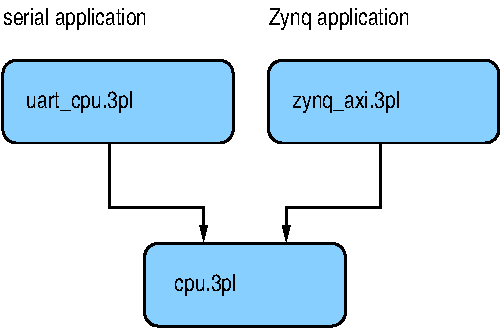
\includegraphics{cpu}

    xilinx/uart\_cpu.3pl is included in -\\
    boards/avnet/aes\_sp3a\_eval400.3pl\\
    board/gadget\_factory/papilio\_one\_100.3pl\\
    board/gadget\_factory/papilio\_one\_250.3pl\\
    board/gadget\_factory/papilio\_one\_500.3pl\\
    board/gadget\_factory/papilio\_pro\_lx4.3pl\\
    board/gadget\_factory/papilio\_pro\_lx9.3pl
    
    uart\_cpu begins by -
    
    \begin{lstlisting}[gobble=4, language=threepl]
    source "xilinx/cpu.3pl"         // CPU API classes file
    class(cpu, CPU_API());          // Create API class here as used below
    global function cpu_api () {    // Pass the API class to application code
        return(cpu);
    }
    \end{lstlisting}
    
    Since cpu.3pl is included via a source statement its code shares the scope
    of this library, UART\_CPU. Thus it can call the modules, functions and
    procedures therin.
    
    {\bf cpu.3pl} defines a class {\bf CPU\_API()} which provides the following
    class procedures for data transfer between FPGA and CPU - \\
        \hspace*{1cm}{\bf read()} generic read \autorefph{sec:lpcpurd} \\
        \hspace*{1cm}{\bf write()} generic write \autorefph{sec:lpcpuwr} \\
        \hspace*{1cm}{\bf read\_memory()} memory read \autorefph{sec:lpcpurdmem} \\
        \hspace*{1cm}{\bf read\_queue()} queue read \autorefph{sec:lpcpurdqueue} \\
        \hspace*{1cm}{\bf read\_value()} value read \autorefph{sec:lpcpurdvalue} \\
        \hspace*{1cm}{\bf write\_memory()} memory write \autorefph{sec:lpcpuwrmem} \\
        \hspace*{1cm}{\bf write\_queue()} queue write \autorefph{sec:lpcpuwrqueue} \\
        \hspace*{1cm}{\bf write\_static()} static write \autorefph{sec:lpcpuwrstat} \\
        \hspace*{1cm}{\bf dma\_read()} to FPGA from CPU \autorefph{sec:lpcpudmar} \\
        \hspace*{1cm}{\bf dma\_write()} from FPGA to CPU \autorefph{sec:lpcpudmaw} \\
        \hspace*{1cm}{\bf signal\_interrupt()} interrupt from a signal \autorefph{sec:lpcpusigint} \\
        \hspace*{1cm}{\bf interrupt()} interrupt procedure \autorefph{sec:lpcpuint} \\

    each of which can generate an instance of a CPU interface to a specific 3PL
    variable of appropriate mode. An internal class {\bf CPU\_CODEGEN} is also
    created but this is not visible to the application code 
    
    cpu.3pl is sourced by both {\bf uart\_cpu.3pl} and {\bf zynq\_axi.3pl} to
    provide CPU interfaces. The former employs a serial data link and the
    latter parallel busses.
    
    When any of the procedures above are called a defining structure is
    created which is added to a list of CPU interfaces. At the end
    of immediate execution module {\bf create\_bus\_interfaces()} is called.
    {\bf create\_bus\_interfaces()} is defined in both {\bf uart\_cpu.3pl}
    and {\bf zynq\_axi.3pl} as it is specific to each. This module
    traverses the interface list constructed above and for each interface
    calls a matching procedure in class {\bf CPU\_CODEGEN} to generate the
    logic for each instance.








    \subsection{library modules}
    



        \subsubsection{cpu\_interface - create the CPU interface low-level logic}\label{sec:lmuartcpui}

            {\bf Library: xilinx/uart\_cpu.3pl)}

            {\bf Prototype:} \\
            \vsp
            \begin{lstlisting}[gobble=12, language=threepl]
                module
                cpu_interface () {}
            \end{lstlisting}
            
            {\bf Output parameters:} \\
            
                none.                       
            
            {\bf Input parameters:} \\
            
                none.
                       
            {\bf description:} \\
            This module is called by module {\bf create\_bus\_interfaces}
            to generate the low-level interface logic to the CPU.




        \subsubsection{create\_bus\_interfaces - create the individual CPU interfaces}\label{sec:lmuartcpucbi}

            {\bf Library: xilinx/uart\_cpu.3pl)}

            {\bf Prototype:} \\
            \vsp
            \begin{lstlisting}[gobble=12, language=threepl]
                module
                create_bus_interfaces () {}
            \end{lstlisting}
            
            {\bf Output parameters:} \\
            
                none.                       
            
            {\bf Input parameters:} \\
            
                none.
                       
            {\bf description:} \\
            This module creates the logic for each of the CPU interfaces. Each
            of these communicates via logic created by module {\bf cpu\_interface}
            described above.







        \subsubsection{dma\_read - DMA read to the FPGA from CPU RAM}\label{sec:lmuartcpudmar}

            {\bf Library: xilinx/uart\_cpu.3pl)}

            {\bf Prototype:} \\
            \vsp
            \begin{lstlisting}[gobble=12, language=threepl]
                module
                dma_read (
                    queue(data)
                    <-
                    queue(address, "uint:16")   // relative memory address
                ) {}
            \end{lstlisting}
            
            {\bf Output parameters:} \\
            
                {\bf data} is the data output queue.                       
            
            {\bf Input parameters:} \\
            
                {\bf address} is a queue supplying the CPU RAM address
                relative to the DMA base address.
                       
            {\bf description:} \\
            This module performs a DMA read to the FPGA from CPU RAM. The
            transfer occurs when input queue {\bf address} is not empty
            and the output queue {\bf data} is not full.\\







        \subsubsection{dma\_write - DMA write from the FPGA to CPU RAM}\label{sec:lmuartcpudmaw}

            {\bf Library: xilinx/uart\_cpu.3pl)}

            {\bf Prototype:} \\
            \vsp
            \begin{lstlisting}[gobble=12, language=threepl]
                module
                dma_write (
                    queue(data),
                    queue(address, "uint:16")   // relative memory address
                ) {}
            \end{lstlisting}
            
            {\bf Output parameters:} \\
            
                none.                       
            
            {\bf Input parameters:} \\
                        
                {\bf data} is the data input queue.\\
                {\bf address} is a queue supplying the CPU RAM address
                relative to the DMA base address.\\
                       
            {\bf description:} \\
            This module performs a DMA write from the FPGA to CPU RAM. The
            transfer occurs when input queues {\bf address} and data are
            not empty.

        \subsubsection{sigint - interrupt the CPU on a signal}\label{sec:lmuartcpusigint}

            {\bf Library: xilinx/uart\_cpu.3pl)}

            {\bf Prototype:} \\
            \vsp
            \begin{lstlisting}[gobble=12, language=threepl]
                module
                sigint(int(n), value(sig, "log")) {}
            \end{lstlisting}
            
            {\bf Output parameters:} \\
            
                none.                       
            
            {\bf Input parameters:} \\
                        
                {\bf n} is the interrupt index, 0 to 16.\\
                {\bf sig} is a signal on whose rising edge the interrupt
                is triggered.\\
                       
            {\bf description:} \\
            When the signal {\bf sig} is asserted the interrupt is triggered.
            The interrupt number, 0 to 15, is given by {\bf index}.


    
    \subsection{library procedures}
            


        \subsubsection{add\_interface - add an interface to the interface list}\label{sec:lpuartcpuai}

            {\bf Library: xilinx/uart\_cpu.3pl)}

            {\bf Prototype:} \\
            \vsp
            \begin{lstlisting}[gobble=12, language=threepl]
                procedure
                add_interface (var(v, "->")) {}
            \end{lstlisting}
            
            {\bf Output parameters:} \\
            
                none.
                       
            {\bf Input parameters:} \\
            {\bf v} is an instance of class {\bf busCommon}, defined in
            cpu.3pl.
                     
            {\bf description:} \\
            The instance of {\bf busCommon} is added to the interface list.
            The list is processed at completion of immediate execution to
            create the whole CPU interface.


        \subsubsection{cpu\_read - write to CPU}\label{sec:lpuartcpurd}

            {\bf Library: xilinx/uart\_cpu.3pl)}

            {\bf Prototype:} \\
            \vsp
            \begin{lstlisting}[gobble=12, language=threepl]
                procedure
                cpu_read (
                    value(access, "log"),
                    value(init, "log"), 
                    queue(out)
                    <-
                    int(bus),
                    int(addr),
                    value(data_in),
                    value(contin, "log")
                ) {}
            \end{lstlisting}
            
            {\bf Output parameters:} \\
            {\bf access} is an optional output parameter which is asserted
            when a CPU to FPGA write occurs.\\
            {\bf init} is an output parameter which is asserted in the case
            of a memory read to initiate the read.\\
            {\bf out} is an optional queue variable which will be written to
            when a transfer occurs.\\

                       
            {\bf Input parameters:} \\
            {\bf bus} is not used (applies to Zynq).\\
            {\bf address} is a 6 bit interface address.\\
            {\bf data\_in} input data.\\
            {\bf contin} is only used for a memory read and is asserted
            when the memory read has occured and the transfer can begin.\\
                     
            {\bf description:} \\
            This procedure provides a low-level interface to transfer
            data from the FPGA to the CPU via the USB serial port. It is
            used by modules and procedures in library cpu.3pl and is not
            intended for use directly by application code.
            
            The CPU initiates the transfer. The transfer may consist of
            multiple bytes.


        \subsubsection{cpu\_write - write to CPU}\label{sec:lpuartcpuwr}

            {\bf Library: xilinx/uart\_cpu.3pl)}

            {\bf Prototype:} \\
            \vsp
            \begin{lstlisting}[gobble=12, language=threepl]
                procedure
                cpu_write (
                    var(out),
                    value(access, "log")
                    <-
                    int(bus),
                    int(addr)
                ) {}
            \end{lstlisting}
            
            {\bf Output parameters:} \\
            {\bf var} is a static or queue mode variable.\\          
            {\bf access} is an optional output parameter which is asserted
            when a CPU to FPGA write occurs.\\
                       
            {\bf Input parameters:} \\
            {\bf bus} is not used (applies to Zynq).\\
            {\bf address} is a 6 bit interface address.\\           
                     
            {\bf description:} \\
            This procedure provides a low-level interface to transfer
            data from the CPU to the FPGA via the USB serial port. It is
            used by modules and procedures in library cpu.3pl and is not
            intended for use directly by application code.
            
            The CPU initiates the transfer. The transfer may consist of
            multiple bytes.



    \subsection{library functions}

        \subsubsection{cpu\_api - CPU communications interface}\label{sec:lfcpuapi}

            {\bf Library: xilinx/uart\_cpu.3pl)}

            {\bf Prototype:} \\
            \vsp
            \begin{lstlisting}[gobble=12, language=threepl]
               global function
               cpu_api () {}
            \end{lstlisting}

            {\bf Return mode and type:} \\
            immediate, class

            {\bf Input parameters:} \\            
            
            none.
            
            {\bf description:} \\
            This function returns an instance of class CPU\_API














\pagebreak

\section{The Standard Library - stdlib.3pl}

    \index{library!stdlib.3pl}
    This library contains modules, procedures and functions common
    to all platforms.
    
    This library must be incorporated by using a {\bf module} statement -
    \begin{lstlisting}[gobble=4, language=threepl]
       module "stdlib.3pl"
    \end{lstlisting}
    
    This library includes {\bf multlib.3pl} and {\bf divlib.3pl}. These are
    not documented separately.

    \subsection{global structs}
        
%        Global struct {\em bram} is created for use with block RAM
%        extended access procedures {\em rwrite2()} and {\em rread2()} and
%        function {\em rmemoryout2()}.
%
%        \begin{lstlisting}[gobble=8, language=threepl]
%           struct(bram,
%               bwidth, "int",  // block data width (in 1st only)
%               twidth, "int",  // total data width (in 1st only)
%               block,  "->",   // memory block
%               next,   "->"    // next bram struct in linked list
%           );
%        \end{lstlisting}
%        
%        Global struct {\em mem\_ad} is created for use with external memory
%        access.
%
%        \begin{lstlisting}[gobble=8, language=threepl]
%           struct (mem\_ad,
%               address,    "uint:20",
%               data,       "bits:18"
%           );
%        \end{lstlisting}
%        
%        It is used by the modules {\bf extramread} and {\bf extramwrite}.
        
        Global structs {\bf ds16}, {\bf ds16e} and {\bf ds32} are
        used for block protocols and for high speed serial channel data.

        \begin{lstlisting}[gobble=8, language=threepl]
           struct(global.ds16,
               data,   "bits:16",  // data word
               k,      "log"       // data word contains K-character in MS byte
           );
        \end{lstlisting}

        \begin{lstlisting}[gobble=8, language=threepl]
           struct(global.ds16e,
               data,   "bits:16",  // data word
               k,      "log",      // data word contains K-character in MS byte
               error,  "log"       // data word is erroneous
           );
        \end{lstlisting}

        \begin{lstlisting}[gobble=8, language=threepl]
           struct(global.ds32,
               data,   "uint:32",  // data word
               k,      "log"       // data word contains K-character in MS byte
           );
        \end{lstlisting}


    \subsection{library modules}
    
        \subsubsection{array\_to\_queue - serialise an array to a
                                                    queue}\label{sec:lmarraytoqueue}


            {\bf Library: stdlib.3pl}

            {\bf Prototype:} \\
            \vsp
            \begin{lstlisting}[gobble=12, language=threepl]
               global module
               array_to_queue (
                   queue(pout),
                   value(busy, "log")
                   <-
                   value(in),
                   value(enable),
                   value(go, "log")
               );
            \end{lstlisting}

            {\bf Output parameters:} \\
            {\bf pout} is the output queue variable\\
            {\bf busy} is true when the module cannot accept another input

            {\bf Input parameters:} \\
            {\bf in} is the input array.\\
            {\bf enable} is an optional argument controlling the number of
            items in {\bf in} to process.\\
            {\bf go} is asserted to trigger the serialisation.

            {\bf description:} \\
            Parameter {\bf in} is an array. It may be value, static, queue,
            selectvalue or priority mode.
            
            Parameter {\bf enable} is a one dimensional array of "log" and may
            be value, static, or selectvalue mode. It must have the same
            dimension as the first or only dimension of parameter {\bf in}.            
            
            When {\bf go} is true the input array is copied to an internal
            structure which is then shifted out to the output queue {\bf pout}.
            The {\bf enable} array indicates which members of array {\bf in} are
            to be copied and shifted, the lowest index false member of {\bf
            enable} indicating that all members of array {\bf in} from that
            index up are ignored. Thus array {\bf enable} must have a number of
            contiguous entries which are true, starting at index 0, and that
            selects the number of contiguous entries in array {\bf in} which
            will be copied and shifter to the output queues, again starting with
            index 0. {\bf go} may contain queue reads.
            
            The second input argument, for parameter {\bf enable}, may be
            omitted in which case all members of {\bf in} will be shifted and
            copied to the output queue.
            
            The output queue must be the same type as the input
            array members. While the serialisation is in progress output value
            {\bf busy} is true. If input {\bf go} is true when {\bf busy} returns to
            false another conversion will take place. If the input {\bf in} is a queue
            then {\bf go} may be held true.
            
            The serialisation takes a number of clock cycles equal to the number
            of entries in the input array that are enabled plus one and hence
            the input data rate is limited to $\frac{1}{n+1}$ where $n$ is the
            number of enabled entries in the input array.



    
        \subsubsection{crc\_8\_16 - 16 bit CRC from 8 bit data}\label{sec:lmcrc816}


            {\bf Library: stdlib.3pl}

            {\bf Prototype:} \\
            \vsp
            \begin{lstlisting}[gobble=12, language=threepl]
               global module
               crc_8_16 (
                   static(out, "uint:16")
                   <-
                   queue(in, "uint:8"),
                   str(poly, "CRC16")
               ) {}
            \end{lstlisting}

            {\bf Output parameters:} \\
            {\bf out} is the output static variable.

            {\bf Input parameters:} \\
            {\bf in} is the input queue.\\
            {\bf poly} is an optional string argument to select the polynomial
            used.

            {\bf description:} \\
            This module accumulate a 16 bit CRC from 8 bit data. Parameter {\bf
            in} is the data input queue, type "uint:8". The CRC is updated as
            each input datum is read. The optional parameter {\bf poly} selects
            one of two polynomials to use. "CRC16" (default) selects $x^{16} +
            x^{15} + x^{13} + 1$. "CCITT" selects $x^{16} + x^{12} + x^5 + 1$. parameter
            {\bf out} is a "uint:16" static variable in which the CRC value is
            accumulated Input data can be read at clock rate.



    
        \subsubsection{crc\_16\_16 - 16 bit CRC from 8 bit data}\label{sec:lmcrc1616}


            {\bf Library: stdlib.3pl}

            {\bf Prototype:} \\
            \vsp
            \begin{lstlisting}[gobble=12, language=threepl]
               global module
               crc_16_16 (
                   static(out, "uint:16")
                   <-
                   queue(in, "uint:16"),
                   str(poly, "CRC16")
               ) {}
            \end{lstlisting}

            {\bf Output parameters:} \\
            {\bf out} is the output static variable.

            {\bf Input parameters:} \\
            {\bf in} is the input queue.\\
            {\bf poly} is an optional string argument to select the polynomial
            used.

            {\bf description:} \\
            This module accumulate a 16 bit CRC from 16 bit data. Parameter {\bf
            in} is the data input queue, type "uint:16". The CRC is updated as
            each input datum is read. The CRC is computed successively from each
            8-bit half of each input datum but in one clock cycle. The optional
            parameter {\bf poly} selects one of two polynomials to use. "CRC16"
            (default) selects $x^{16} + x^{15} + x^{13} + 1$. "CCITT" selects
            $x^{16} + x^{12} + x^5 + 1$. parameter {\bf out} is a "uint:16"
            static variable in which the CRC value is accumulated Input data can
            be read at clock rate.








    
        \subsubsection{crcblock - block 32 bit data with a CRC}\label{sec:lmcrcblock}


            {\bf Library: stdlib.3pl}

            {\bf Prototype:} \\
            \vsp
            \begin{lstlisting}[gobble=12, language=threepl]
               global module
               crcblock (
                   queue(out, ds16)
                   <-
                   queue(in, ds32),
                   int(max_blk_len, 20),
                   int({sob, eob}),
                   log(fixed)
               ) {}
            \end{lstlisting}

            {\bf Output parameters:} \\
            {\bf out} is the output queue, type ds16.

            {\bf Input parameters:} \\
            {\bf in} is the input queue, type ds32.\\
            {\bf max\_blk\_len} is the maximum variable block size or the fixed
                    block size.\\
            {\bf sob} is the start-of-block K-character to be used.\\
            {\bf eob} is the end-of-block K-character to be used.\\
            {\bf fixed} is an optional logical argument to select fixed
                    length blocks.

            {\bf description:} \\
            This module encloses data in a block containing a cyclic reduncancy
            check word. The 16 bit CRC polynomial is $x^{16} + x^{15} + x^{13} +
            1$. Blocks can be fixed or variable length.

            When input data become available the start-of-block word is written
            to the output queue. The start-of-block word has the most significant
            byte set to the start-of-block K character, the least significant
            byte to zero and the K flag is true. If 'fixed' is false (default),
            incoming data is read until either unavailable or max\_block\_len
            items have been read and the block is then terminated. If 'fixed' is
            true, incoming data is read until max\_block\_len items have been
            read and the block is then terminated. each 32 bit word is written
            to the output as a pair of 16 bit words. A 16 bit CRC is accumulated
            from each 16 bit data word. When the block is terminated the 16 bit
            CRC is written to the output followed by an end-of-block word. The
            end-of-block word has the most significant byte set to the
            end-of-block K character, the least significant byte to zero and the
            K flag is true.

            \begin{tabular}{| c | c | c | l}
            \cline{1-3}
            K & upper & lower & \\
            flag & byte & byte & \\
            \cline{1-3}
            \cline{1-3}
            1 & sob &  0  & start-of-block \\ \cline{1-3}
            0 & \multicolumn{2}{| c |}{data word 1} & first data word \\ \cline{1-3}
            0 & \multicolumn{2}{| c |}{data word 2} & second data word \\ \cline{1-3}
            . & \multicolumn{2}{| c |}{.} &  \\
            . & \multicolumn{2}{| c |}{.} &  \\ \cline{1-3}
            0 & \multicolumn{2}{| c |}{data word n} & last data word \\ \cline{1-3}
            0 & \multicolumn{2}{| c |}{CRC} & CRC \\ \cline{1-3}
            1 & eob &  0  & end-of-block \\ \cline{1-3}
            \end{tabular}








    
        \subsubsection{crcunblock - unblock 32 bit data with a CRC}\label{sec:lmcrcunblock}


            {\bf Library: stdlib.3pl}

            {\bf Prototype:} \\
            \vsp
            \begin{lstlisting}[gobble=12, language=threepl]
               global module
               crcunblock (
                   queue(dout, ds32),
                   static(eout)
                   <-
                   queue(in, ds16),
                   int(max_blk_len, 20),
                   int({sob, eob})
               ) {}
            \end{lstlisting}

            {\bf Output parameters:} \\
            {\bf out} is the output queue, type ds32.\\
            {\bf eout} is an optional error counter static variable.

            {\bf Input parameters:} \\
            {\bf in} is the input queue, type ds16.\\
            {\bf max\_blk\_len} is the maximum variable block size or the fixed
                    block size.\\
            {\bf sob} is the start-of-block K-character to be used.\\
            {\bf eob} is the end-of-block K-character to be used.

            {\bf description:} \\
            This module unwraps data from a block containing a cyclic reduncancy
            check word. The 16 bit CRC polynomial is $x^{16} + x^{15} + x^{13} +
            1$. Blocks can be fixed or variable length. The start-of-block word,
            CRC word and end-of-block word are stripped off the input stream and
            data words are packed into 32 bit words (ds32 struct). A CRC is
            computed from the block data including the transmitted CRC word. If
            the resulting CRC is zero the block is written to the output queue.
            If the CRC is not zero the block is discarded.
            
            When a block CRC error is encountered if the output parameter 'eout'
            has an argument the data length of the discarded block is added to
            the value of that variable. Any words received that do not match the
            block format cause 'eout' to be incremented. The size of the 'eout'
            counter is determined by the argument passed in the call to
            crcunblock().

            If the block length exceeds the maximum block length the block is
            terminated and discarded and if the optional error counter output
            parameter is used, the block length is added to the error count.

            Unpacked data is written to a dual-port circular buffer so that
            completed correct data words can be copied to the output data queue
            in parallel with unpacking of incoming blocks. If the output queue
            becomes unavailable for writing, data words will be discarded.


    
  
        \subsubsection{cread - read combinatorial output memory to a
                                                        queue}\label{sec:lmcread}

            {\bf Library: stdlib.3pl}


            {\bf Prototype:} \\
            \vsp
            \begin{lstlisting}[gobble=12, language=threepl]
               global module
               cread (queue(data) <- rmemory(m), int(port), queue(addr)) {}
            \end{lstlisting}

            {\bf Output parameters:} \\
            {\bf data} is the queue variable to be written to from the memory
            read. It takes its type from the argument.

            {\bf Input parameters:} \\
            {\bf m} is the memory.\\
            {\bf port} is the memory port.\\
            {\bf addr} is the memory address.

            {\bf description:} \\
            Read the combinatorial output memory when the input and output
            queues are available. The program logic must ensure that this
            memory port access is mutually exclusive to all other accesses
            to that port.
            
            This module is just a wrapper around a single statement. The source
            is
            \begin{lstlisting}[gobble=12, language=threepl]
               global module
               cread (queue(data) <- rmemory(m), int(port), queue(addr)) {
                   data <<- cast(cmemoryread(m, port, addr), type(data));
               }
            \end{lstlisting}
                        
            It is provided to complete the set {\bf cread()}, {\bf cwrite()},
            {\bf rread()} and {\bf rwrite()} where only rread() contains
            significant code.
            
            See also - \\
            {\bf cwrite()} \autorefph{sec:lmcwrite}, \\
            {\bf rread()} \autorefph{sec:lmrread}, \\
            {\bf rwrite()} \autorefph{sec:lmrwrite}.

    
        \subsubsection{cwrite - write combinatorial output memory from a
                                                    queue}\label{sec:lmcwrite}

            {\bf Library: stdlib.3pl}

            {\bf Prototype:} \\
            \vsp
            \begin{lstlisting}[gobble=12, language=threepl]
               global module
               cwrite (rmemory(m), int(port), queue({addr, data})) {}
            \end{lstlisting}

            {\bf Output parameters:} \\
            none

            {\bf Input parameters:} \\ 
            {\bf m} is the memory.\\
            {\bf port} is the memory port.\\
            {\bf addr} is the memory address.\\            
            {\bf data} is the data to be written.

            {\bf description:} \\
            Write to the combinatorial output memory when the input queues are
            available. The program logic must ensure that this memory port
            access is mutually exclusive to all other accesses to that port.
            
            This module is just a wrapper around a single statement. The source
            is
            \begin{lstlisting}[gobble=12, language=threepl]
               global module
               cwrite (rmemory(m), int(port), queue(addr), queue(data)) {
                   cmemorywrite(m, port, addr, data);
               }
            \end{lstlisting}
                        
            It is provided to complete the set {\bf cread()}, {\bf cwrite()},
            {\bf rread()} and {\bf rwrite()} where only rread() contains
            significant code.
            
            See also - \\
            {\bf cread()} \autorefph{sec:lmcread}, \\
            {\bf rread()} \autorefph{sec:lmrread}, \\
            {\bf rwrite()} \autorefph{sec:lmrwrite}.





        \subsubsection{demultiplex - demultiplex a source\\
                    demultiplex\_l - demultiplex a source using port bit\\
                    demultiplex\_e - demultiplex a source using port number}\label{sec:lmdemultiplex}

            {\bf Library: stdlib.3pl}

            {\bf Prototypes:} \\
            \vsp
            \begin{lstlisting}[gobble=12, language=threepl]
               global module
               demultiplex.... (varargs <- queue(in)) {}
            \end{lstlisting}

            {\bf Output parameters:} \\
            {\bf varargs} any number of output sinks, an array of pointers
            to sinks or a list of sinks.

            {\bf Input parameters:} \\
            {\bf in} is a single input queue.

            {\bf description:} \\
            These modules are intended to demultiplex a single input queue to a
            number of output queues. Outputs need not be the same type but they must
            be assignable from the input type (or {\bf body} field of the input -
            see below). The input need not contain queue reads in which case it will
            be read on every clock cycle.

            These modules may also be called with a single output argument which
            is an array of pointers to queues. In this case they behave as though
            called with the queues as separate arguments. Similarly the single
            output argument may be of type "list", the list containing pointers
            to queues.

            The output types must be a type assignable from the input data
            type. By 'assignable' is meant that the types need not be identical,
            e.g. the number of bits may differ in which case truncation or
            padding will occur or a "uint" may be assigned to an "int".

            For {\bf demultiplex()} the input can be any type. The input is
            copied to the outputs in turn. If an output is not available the
            next available output in cyclic order is selected. If no outputs
            are available the module waits until any output is available and
            this is written to.

            For {\bf demultiplex\_l()} the input type is a wrapper struct
            containing the datum and an output port identifier. That identifier
            is an array of type "log" in which one member is {\bf true} to
            identify the output port. The struct can be created by calling the
            library global function {\bf multiplex\_struct\_l()}
            \autorefph{sec:lfmultiplexstruct}.

            For {\bf demultiplex\_e()} the input type is a wrapper struct
            containing the datum and an output port identifier. That identifier
            is  a "uint" containing the port number (starting at 0). The struct
            can be created by calling the library global function {\bf
            multiplex\_struct\_e()} \autorefph{sec:lfmultiplexstruct}.

            If the selected output queue is an unmatched parameter then the input is
            still read but the data is discarded. For {\bf demultiplex\_l()} and
            {\bf demultiplex\_e()} the directive "demultiplex\_skip\_null\_outputs"
            can be set to true to ignore any unmatched output parameters, but note
            that if an input is directed to that output port the input will not be
            read.

            These modules read and write in the current clock domain.
            Input and output queues may be asynchronous.
            
            The module {\bf demultiplex()} operates by means of a token placed
            on one output. When the input becomes available the first available
            output downstream of the token is written and the token is moved to
            the output following the one written. There are no clock cycles
            lost, as in a traditional token ring, in waiting for the token to
            move around the ring to an available output, thus the module is
            capable of forwarding an input datum on every clock cycle. The
            implementation uses the Xilinx carry chain to minimise the delay
            through the logic cascade of the token ring. If the carry chain were
            not used the logic delays would severely limit the clock rate at
            which this module could be used. Modules {\bf demultiplex\_l()} and
            {\bf demultiplex\_e()} do not need the token ring as the required
            output is explicitly specified by the input.

            
            See also - \\
            {\bf multiplex()} \autorefph{sec:lmmultiplex} \\
            {\bf multiplex\_l()} \autorefph{sec:lmmultiplex} \\
            {\bf multiplex\_e()} \autorefph{sec:lmmultiplex} \\
            {\bf multiplexp()} \autorefph{sec:lmmultiplex} \\
            {\bf multiplexp\_l()} \autorefph{sec:lmmultiplex} \\
            {\bf multiplexp\_e()} \autorefph{sec:lmmultiplex} \\
            {\bf multiplext()} \autorefph{sec:lmmultiplex} \\
            {\bf multiplext\_l()} \autorefph{sec:lmmultiplex} \\
            {\bf multiplext\_e()} \autorefph{sec:lmmultiplex} \\
            {\bf multiplex\_struct\_l()} \autorefph{sec:lfmultiplexstruct} \\
            {\bf multiplex\_struct\_e()} \autorefph{sec:lfmultiplexstruct}.



        \subsubsection{divide - pipeline divide}\label{sec:lmdivide}

            {\bf Library: stdlib.3pl}

            {\bf Prototype:} \\
            \vsp
            \begin{lstlisting}[gobble=12, language=threepl]
               global module
               divide (queue(quot), queue(rem) <- value(num), value(denom)) {}
            \end{lstlisting}

            {\bf Output parameters:} \\
            {\bf quot} is the quotient.\\
            {\bf rem} is the remainder.

            {\bf Input parameters:} \\
            {\bf num} is the dividend.\\
            {\bf denom} is the divisor.
            
            This module is in divlib.3pl which is included in stdlib.3pl.

            {\bf description:} \\
            This module is a pipeline divider. The numerator and denominator
            arguments may be int, uint, int:, uint:, fixed: or ufixed: where the
            trailing ":" indicates target types. For integer types the quotient
            and remainder outputs are integer, signed if either input is signed,
            and either or both the quotient and remainder outputs may be used.
            For one or both inputs fixed point the quotient output will be fixed
            point, signed if either input is signed, and the remainder output
            is not used.
            
            If neither input is a queue or an expression containing a queue the
            divider will accept input on every clock cycle. Either input may be
            immediate mode but both inputs must not be immediate mode. The
            quotient and remainder will become available at the outputs after a
            latency which is determined by the numerator width. Data in transit
            through the module will continue to the outputs regardless of the
            availability of further input data.

            The remainder queue output argument should be at least as wide as the
            denominator argument otherwise the resulting truncation may lose
            data (if the range is known to be constrained then this is
            acceptable).

            For unsigned integer divide (both numerator and denominator
            arguments unsigned target types or non-negative immediate) the
            result width is the width of the numerator argument.

            For signed integer divide (either or both numerator or denominator
            arguments int target types or negative immediate) the result width
            will be one bit wider than for unsigned divide. The extra bit is
            only required for the single case where both numerator and
            denominator are the maximum negative values (e.g. -8 / -1 gives +8,
            but -8 has a width of 4 bits and +8 as a signed int has a width of 5
            bits). If this case is known not to arise a narrower output queue may
            be used.
            
            For fixed point divide the result width is the sum of the numerator
            and denominator widths and the result binary point offset is
            the numerator offset + denominator width - denominator offset.

            The number of pipeline stages is equal to the number of bits in the
            numerator plus one.

            Divide by zero is not detected and gives an undefined result.





        \subsubsection{fifo - a fifo with static interface}\label{sec:lmfifo}

            {\bf Library: stdlib.3pl}

            {\bf Prototype:} \\
            \vsp
            \begin{lstlisting}[gobble=12, language=threepl]
               global module
               fifo (
                   value(out), value({emptyout, fullout}, "log")
                   <-
                   value(in), value({read, write}, "log")
               ) {}
            \end{lstlisting}

            {\bf Output parameters:} \\
            {\bf out} is the data output for a fifo read.\\
            {\bf emptyout} is true if the fifo is empty.\\
            {\bf fullout} is true if the fifo is full.

            {\bf Input parameters:} \\
            {\bf in} is the data input for a fifo write.\\
            {\bf read} causes a fifo read on a clock cycle when high.\\
            {\bf write} causes a fifo write on a clock cycle when high.

            {\bf description:} \\
            Read or write a fifo. On each clock cycle {\bf emptyout} and {\bf
            fullout} indicate when reads and writes respectively cannot be
            executed. The program must ensure that these conditions are
            checked as the module does not do so! If {\bf read} or {\bf
            write} are high in a clock cycle then a read or write will be
            performed. These can be done on the same clock cycle.





        \subsubsection{multiplex - multiplex sources\\
                    multiplex\_l - multiplex sources giving port bit\\
                    multiplex\_e - multiplex sources giving port number\\
                    multiplexp - multiplex queues with priority\\
                    multiplexp\_l - multiplex queues with priority giving port bit\\
                    multiplexp\_e - multiplex queues with priority giving port number\\
                    multiplext - multiplex queues via a tree\\
                    multiplext\_l - multiplex queues via a tree giving port bit\\
                    multiplext\_e - multiplex queues via a tree giving port number}\label{sec:lmmultiplex}

            {\bf Library: stdlib.3pl}

            {\bf Prototype:} \\
            \vsp
            \begin{lstlisting}[gobble=12, language=threepl]
               global module
               multiplex.... (queue(out) <- varargs) {}
            \end{lstlisting}

            {\bf Output parameters:} \\
            {\bf out} is a single output queue.

            {\bf Input parameters:} \\
            {\bf varargs} any number of input sources, an array of pointers
            to sources or a list of sources.

            {\bf description:} \\
            These modules are intended to multiplex a number of input queues to a
            single output queue. Inputs need not be the same type but they must
            be assignable to the output type (or {\bf body} field of the output
            queue - see below). By 'assignable' is meant that the types need not
            be identical, e.g. the number of bits may differ in which case
            truncation or padding will occur or a "uint" may be assigned to an
            "int".          
            
            When inputs become available simultaneously modules {\bf
            multiplex()}, {\bf multiplex\_l()} and {\bf multiplex\_e()} use a
            pseudo-token ring to give equal treatment to all inputs. Note that
            although these modules were written to multiplex queues (or more
            correctly expressions containing queue reads), the input arguments
            could be other modes, say value or static. Where no queue reads are
            involved an expression is always available. In that case the inputs
            would be sampled and copied to the output queue continuously in a
            cyclic order. In principle the inputs could be a mixture of modes in
            which case they would be read cyclically but a queue would be skipped
            if not available for reading.

            Modules {\bf multiplexp()}, {\bf multiplexp\_l()} and {\bf
            multiplexp\_e()} handle simultaneous inputs by choosing the
            left-most available queue in the argument list. For these modules the
            inputs must contain queue reads.

            Modules {\bf multiplext()}, {\bf multiplext\_l()} and {\bf
            multiplext\_e()} handle simultaneous inputs by means of a balanced tree
            structure.
            
            All nine modules may also be called with a single input argument
            which is an array of pointers to sources. In this case they behave
            as though called with the sources as separate arguments. Similarly
            the single input argument may be of type "list", the list containing
            pointers to sources.
            
            In many applications it is necessary to be able to identify the
            origin of an output datum, i.e. the input argument to the module
            from which the datum was read. To facilitate this the module output
            queue type may be a struct which is a wrapper containing the output
            datum and an input port identifier. The output type for {\bf
            multiplex()} and {\bf multiplexp()} do not use a wrapper type, the
            output type being directly compatible with the input type(s).
            
            The output type for {\bf multiplex\_l()}, {\bf multiplexp\_l()} and
            {\bf multiplext\_l()} is a wrapper with two field, {\bf body}
            containing the datum and {\bf port}  which is an array of type "log"
            in which one member is {\bf true} to identify the input port. The
            struct can be created by calling the library global function {\bf
            multiplex\_struct\_l()} \autorefph{sec:lfmultiplexstruct}.
            
            The output type for {\bf multiplex\_e()}, {\bf multiplexp\_e()} and
            {\bf multiplext\_e()} is a wrapper with two fields, {\bf body}
            containing the datum and {\bf port}  which is a "uint" containing
            the port number (starting at 0). The struct can be created by
            calling the library global function {\bf multiplex\_struct\_e()}
            \autorefph{sec:lfmultiplexstruct}.
            
            In the case of {\bf multiplex()}, {\bf multiplexp()} and {\bf
            multiplext()} the inputs are copied to the output queue when
            available. For {\bf multiplex\_l()}, {\bf multiplexp\_l()} and {\bf
            multiplext\_l()} the selected input is copied to the {\bf body}
            field output queue when available and the associated port field has
            the member of the array indexed by the port number assigned true.
            For {\bf multiplex\_e()}, {\bf multiplexp\_e()} and {\bf
            multiplext\_e()} the same applies except that the port number is
            assigned to the "uint" {\bf port} field.
            
            The modules read and write in the current clock domain. Input
            and output queues may be asynchronous.
            
            The modules {\bf multiplex()}, {\bf multiplex\_l()} and {\bf
            multiplex\_e()} operate by means of a token placed on one input.
            When one or more inputs become available the first input downstream
            of the token is read and the token is moved to the input following
            the one read. There are no clock cycles lost, as in a traditional
            token ring, in waiting for the token to move around the ring to an
            available input, thus the module is capable of forwarding an input
            datum on every clock cycle. The implementation uses the Xilinx carry
            chain to minimise the delay through the logic cascade of the token
            ring. Unfortunately the carry chain must be circular and the link
            back from the top of a linear carry chain to the bottom introduces
            a significant delay. The propagation time around the token ring
            is large enough to severely lower the clock rate that can be used
            as the number of inputs increases.
            
            The modules {\bf multiplexp()}, {\bf multiplexp\_l()} and {\bf
            multiplexp\_e()} use a priority mode variable to select which input
            to read. For FPGAs priority mode variables are implemented using the
            Xilinx carry chain if the number of inputs exceeds the maximum
            number of LUT inputs. This is to minimise the delay through cascaded
            logic.
            
            The modules {\bf multiplext()}, {\bf multiplext\_l()} and {\bf
            multiplext\_e()} use a balanced tree with nodes of degree 2 to
            converge the inputs to the output. Each tree node arbitrates between
            its two inputs based on the number of leaves converging on each
            branch. The disadvantage of this scheme is that arbitration is
            based on the fixed configuration, not on the traffic through
            each branch. For example a four input multiplexer where
            input 4 is idle will arbitrate among the other three unfairly
            giving input 3 half the clock cycles, inputs 1 and 2 sharing the
            other half. The advantage of this multiplexer is that it will
            operate at a high clock rate since the arbitration is local to
            the nodes.
                        
            See also - \\
            {\bf demultiplex()} \autorefph{sec:lmdemultiplex} \\
            {\bf demultiplex\_l()} \autorefph{sec:lmdemultiplex} \\
            {\bf demultiplex\_e()} \autorefph{sec:lmdemultiplex} \\
            {\bf multiplex\_struct\_l()} \autorefph{sec:lfmultiplexstruct} \\
            {\bf multiplex\_struct\_e()} \autorefph{sec:lfmultiplexstruct}.
        




        \subsubsection{multiply - pipelined multiply}\label{sec:lmmultiply}

            {\bf Library: stdlib.3pl}

            {\bf Prototype:} \\
            \vsp
            \begin{lstlisting}[gobble=12, language=threepl]
               global module
               multiply (queue(prod) <- value(m1), value(m2)) {}
            \end{lstlisting}

            {\bf Output parameters:} \\
            {\bf prod} is the product.

            {\bf Input parameters:} \\
            {\bf m1} is the multiplicand.\\
            {\bf m2} is the multiplier.
            
            This module is in multlib.3pl which is included in stdlib.3pl.

            {\bf description:} \\
            This module is a pipeline multiplier for signed or unsigned
            integers. The module is useful for Virtex, Virtex E and Spartan 2
            FPGAs which do not contain hardware multipliers. Later Virtex and
            Spartan3 FPGAs containing hardware multipliers offer no reason to
            use this module.
            
            If neither input is a queue or an expression containing a queue the
            multiplier will accept input on every clock cycle unless the output
            queue becomes unavailable. Either input may be a constant but both
            inputs must not be constant. If either input is signed (a target int
            or a -ve constant) the output queue must be signed (an int, not a
            uint).

            The product will become available at the output after a latency
            which is determined by the input widths. Data in transit through the
            module will continue to the output regardless of the availability of
            further input data. The number of pipeline stages depends on the
            size and types of input arguments as follows -

            \begin{tabular}{ l l l }
            unsigned  & expr x expr     & bits in smallest expr \\
            signed    & expr x expr     & bits in smallest expr + 1 \\
            unsigned  & expr x constant & 1-bits in constant \\
            signed    & expr x constant & 1-bits in constant + 1 \\
            \end{tabular}
            
            where signed means that either input argument is signed. {\bf
            expr} means a target variable or expression, possibly containing
            queues. {\bf constant} means an immediate constant, variable or
            expression. Either input argument may be the constant.
            
            The width of the output queue argument should be at least the sum
            of the widths of the two input arguments. If narrower the result
            will be truncated at the most significant end. If the range of
            the product is known to be constrained then truncation of the
            product is acceptable.
            
            


        \subsubsection{pfifo - a prewrite fifo with static interface}\label{sec:lmpfifo}

            {\bf Library: stdlib.3pl}

            {\bf Prototype:} \\
            \vsp
            \begin{lstlisting}[gobble=12, language=threepl]
               global module
               pfifo (
                   value(out),
                   value({emptyout, fullout}, "log")
                   <-
                   value(in),
                   value({read, prewrite, write}, "log"),
                   value(reset, "log")
               ) {}
            \end{lstlisting}

            {\bf Output parameters:} \\
            {\bf out} is the data output for a fifo read.\\
            {\bf emptyout} is true if the fifo is empty.\\
            {\bf fullout} is true if the fifo is full.

            {\bf Input parameters:} \\
            {\bf in} is the data input for a fifo write.\\
            {\bf read} causes a fifo read on a clock cycle when high.\\
            {\bf prewrite} notifies the fifo that a write will be done
            in the future, reserving a place. When no free places remain the
            full condition will be come true.\\
            {\bf write} causes a fifo write on a clock cycle when high. The
            empty condition takes account of data actually written, not
            notified writes (prewrites).\\
            {\bf reset} is an optional reset to clear the fifo.

            {\bf description:} \\
            This fifo is intended to be used where data is to be passed
            through a fifo but there is a delay between execution of the
            data-producing operation and availability of that data. An
            example of this is external memory reads where the data only
            becomes available a number of cycles after the read command has
            been sent. The resulting data are then to be buffered in this
            fifo. To ensure that the memory reads can be pipelined it is
            necessary to notify the fifo that a write will occur later so
            that its test for space can take that into account. Once the
            memory read has been signaled it cannot be stopped so the fifo
            must have space available for the resulting datum some cycles
            later.
            
            On each clock cycle {\bf emptyout} and {\bf fullout} indicate
            when reads and writes respectively cannot be executed. The
            program must ensure that these conditions are checked as the
            module does not do so! If {\bf read}, {\bf prewrite} or {\bf
            write} are high in a clock cycle then a read, prewrite or write
            will be performed. Any combination of these can all occur on
            one clock cycle.


        \subsubsection{pdelay - delay pipeline data}\label{sec:lmpdelay}

            {\bf Library: stdlib.3pl}

            {\bf Prototype:} \\
            \vsp
            \begin{lstlisting}[gobble=12, language=threepl]
               global module
               pdelay (
                   queue(out)
                   <-
                   queue(in),
                   int(delay),
                   value(reset, "log")
               ) {}
            \end{lstlisting}

            {\bf Output parameters:} \\
            {\bf out} is the data output.

            {\bf Input parameters:} \\
            {\bf in} is the data input.\\
            {\bf delay} is the numnber of data to be delayed.\\
            {\bf reset} is an optional reset.

            {\bf description:} \\
            This module delays data by the number specified by argument
            {\bf delay}. The module will only operate when both input
            and output queues are available. Initially {\em delay} input data
            will be consumed while outputing default values (0, false etc.).
            Following this the output datum will be that input {\em delay}
            data cycles ago. The optional reset can be used to return the
            module to its initial condition.


        \subsubsection{rread - read registered output memory to a
                                                    queue}\label{sec:lmrread}

            {\bf Library: stdlib.3pl}

            {\bf Prototype:} \\
            \vsp
            \begin{lstlisting}[gobble=12, language=threepl]
               global module
               rread (queue(data) <- rmemory(m), int(port), queue(addr)) {}
            \end{lstlisting}

            {\bf Output parameters:} \\
            {\bf data} is the queue variable to be written to from the memory
            read. It takes its type from the argument.

            {\bf Input parameters:} \\
            {\bf m} is the memory.\\
            {\bf port} is the memory port.\\
            {\bf addr} is the memory address.

            {\bf description:} \\
            Read the registered output memory when the input and output
            queues are available. There is a latency of 2 cycles between input
            and output.
            
            The program logic must ensure that this
            memory port access is mutually exclusive to all other accesses
            to that port.
            
            See also - \\
            {\bf cread()} \autorefph{sec:lmcread}, \\
            {\bf cwrite()} \autorefph{sec:lmcwrite}, \\
            {\bf rwrite()} \autorefph{sec:lmrwrite}.


        \subsubsection{rwrite - write registered output memory from a
                                                    queue}\label{sec:lmrwrite}

            {\bf Library: stdlib.3pl}

            {\bf Prototype:} \\
            \vsp
            \begin{lstlisting}[gobble=12, language=threepl]
               global module
               rwrite (rram(m), int(port), queue({addr, data})) {}
            \end{lstlisting}

            {\bf Output parameters:} \\
            none

            {\bf Input parameters:} \\
            {\bf m} is the memory.\\
            {\bf port} is the memory port.\\
            {\bf addr} is the memory address.\\            
            {\bf data} is the data to be written.

            {\bf description:} \\
            Write to the registered output memory when the input queues are
            available. The program logic must ensure that this memory port
            access is mutually exclusive to all other accesses to that port.

            The registered output of the port is also changed to the written
            value.
            
            This module is just a wrapper around a single statement. The source
            is
            \begin{lstlisting}[gobble=12, language=threepl]
               global module
               rwrite (rmemory(m), int(port), value(addr), value(data)) {
                   rmemorywrite(m, port, addr, data);
               }
            \end{lstlisting}
                        
            It is provided to complete the set {\bf cread()}, {\bf cwrite()},
            {\bf rread()} and {\bf rwrite()} where only rread() contains
            significant code.
            
            See also - \\
            {\bf cread()} \autorefph{sec:lmcread}, \\
            {\bf cwrite()} \autorefph{sec:lmcwrite}, \\
            {\bf rread()} \autorefph{sec:lmrread}.


        \subsubsection{sort - generate a parallel Batcher sort network}\label{sec:lmsort}

            {\bf Library: stdlib.3pl}

            {\bf Prototype:} \\
            \vsp
            \begin{lstlisting}[gobble=12, language=threepl]
               global module
               sort (queue(out) <- queue(in)) {}
            \end{lstlisting}

            {\bf Output parameters:} \\
            {\bf out} is the output queue.

            {\bf Input parameters:} \\
            {\bf in} is the input queue.

            {\bf description:} \\
            This module generates a parallel sort network. The input and output
            arguments are queues which are 1-dimensional arrays of type uint or
            int. The output ordering depends on the The input and output array
            dimensions and types must be the same. The number of pipeline
            stages in this module depends on the dimensions of the queues. The
            sort network is generated using Batcher's algorithm. Note that the
            amount of logic used grows rapidly with the dimensionality of the
            queues!



        \subsubsection{sqrt - target fixed point square root}\label{sec:lmsqrt}

            {\bf Library: stdlib.3pl}

            {\bf Prototype:} \\
            \vsp
            \begin{lstlisting}[gobble=12, language=threepl]
               global module
               sqrt (queue(out) <- queue(in)) {}
            \end{lstlisting}

            {\bf Output parameters:} \\
            {\bf out} is the output queue.

            {\bf Input parameters:} \\
            {\bf in} is the input queue.

            {\bf description:} \\
            This module performs a bitwise iterative square root on an unsigned
            integer or unsigned fixed point value. The input and output
            arguments must be queue mode variables. The input and output types
            must be both "uint:" or both "ufixed:". The integer or fractional
            widths of input and output need not match. For integers the output
            width will usually be half the input width. For fixed point the
            output type would usually have the point moved left with respect to
            the input. If a result value exceeds the integer or fractional width
            of the output type, left or right truncation will occur.

            Where the operand is not an exact square the result is truncated at
            the least significant end, i.e. the result is the largest value
            whose square is not larger than the operand.
            
            The module does not process data at clock rate; it processes an
            operand in a fixed time of n/2+2 clock cycles where 'n' is the width
            of the (internal) operand.
            
            For an integer square root 'n' is the width of the input, plus 1
            if the width is odd.
            
            For a fixed point square root 'n' is calculated as follows -
            \begin{lstlisting}[gobble=12, language=threepl]
               int(n, size(in));       // total operand width - initially that of input
               int(ifb, offset(in));   // input fraction part width
               int(iib, n - ifb);      // input integer part width
               int(ioffset);           // input left offset to form internal integer
               int(ofb, offset(out));  // output fraction part width
               int(xoffset);           // extra offset for more fractional precision

               if ((ifb % 2) != 0) {   // if input fractional part width odd --
                   n++;                // increment n to make even
                   ioffset = 1;        // input must now be offset by 1 bit
               }
               xoffset = (2 * ofb) - (ifb + ioffset); // extra precision for output fractional part
               if (xoffset > 0) {      // if extra width for output fractional precision --
                   n += xoffset;       // add to n
                   ioffset += xoffset; // add to input offset
               }
               if ((n % 2) != 0)   // if total width odd --
                   n++;            // increment n to make even
            \end{lstlisting}
            This increments n for either integer or fraction part of odd width
            and also widens the the internal operand to account for extra
            precision in the output fractional part compared to the input.
            
            



        \subsubsection{stretch - generate a long pulse from a transition}\label{sec:lmstretch}

            {\bf Library: stdlib.3pl}

            {\bf Prototype:} \\
            \vsp
            \begin{lstlisting}[gobble=12, language=threepl]
               global module
               stretch (static(out, "log") <- value(in, "log"), int(n)) {}
            \end{lstlisting}

            {\bf Output parameters:} \\
            {\bf out} is the output static variable.

            {\bf Input parameters:} \\
            {\bf in} is the input value.\\
            {\bf n} is the required length of the output pulse.

            {\bf description:} \\
            When input argument {\bf in} goes from false to true generate an
            output {\bf out} which is true for the number of cycles specified
            by argument {\bf n}.


        \subsubsection{timebase - generate decadic pulses}\label{sec:lmtimebase}

            {\bf Library: stdlib.3pl}

            {\bf Prototype:} \\
            \vsp
            \begin{lstlisting}[gobble=12, language=threepl]
               global module
               timebase(
                   static({tb_1us, tb_10us, tb_100us, tb_1ms, tb_10ms, tb_100ms, tb_1s}, "log")
                   <-
               ) {}
            \end{lstlisting}

            {\bf Output parameters:} \\
            {\bf tb\_1us} is a $1\mu S$ interval pulse stream. \\
            {\bf tb\_10us} is  a $10\mu S$ interval pulse stream. \\
            {\bf tb\_100us} is  a $100\mu S$ interval pulse stream. \\
            {\bf tb\_1ms} is  a $1mS$ interval pulse stream. \\
            {\bf tb\_10ms} is  a $10mS$ interval pulse stream. \\
            {\bf tb\_100ms} is  a $100mS$ interval pulse stream. \\
            {\bf tb\_1s} is  a $1S$ interval pulse stream. 

            {\bf Input parameters:} \\
            None.

            {\bf description:} \\
            This module generates pulse streams at decade intervals of $1\mu S$
            up to $1S$. Each pulse is one cycle in the current clock domain.
            Each output pulse is aligned with the pulses from higher frequency
            outputs. The current clock frequency must be $\ge$ 2MHz.
            
            The $1\mu S$ pulses are derived from the current clock by integer
            division and hence if the current clock is not an integer
            multiple of 1MHz the interval will differ from $1\mu S$. Each of
            the other outputs is derived from the next higher frequency
            output by division by 10.


        \subsubsection{to\_pulse - generate a pulse from a
                                                    transition}\label{sec:lmtopulse}

            {\bf Library: stdlib.3pl}

            {\bf Prototype:} \\
            \vsp
            \begin{lstlisting}[gobble=12, language=threepl]
               global module
               to_pulse (static(out, "log") <- value(in, "log")) {}
            \end{lstlisting}

            {\bf Output parameters:} \\
            {\bf out} is the output static variable.

            {\bf Input parameters:} \\
            {\bf in} is the input value.

            {\bf description:} \\
            Generate a pulse on {\bf out} when the input argument {\bf in}
            changes from false to true.



        \subsubsection{tws\_recv - two wire serial receiver}\label{sec:lmtwsrecv}

            {\bf Library: stdlib.3pl}


            {\bf Prototype:} \\
            \vsp
            \begin{lstlisting}[gobble=12, language=threepl]
               tws_recv(
                   queue(out)
                   <-
                   value(sck, "log"), value(sdo, "log"), varargs
               ) {}
            \end{lstlisting}

            {\bf Output parameters:} \\
            {\bf out} is the output queue variable.

            {\bf Input parameters:} \\
            {\bf sck} is the input serial clock. \\
            {\bf sdo} is the input serial data. \\
            {\bf varargs} matches two optional arguments, {\bf silence} and
            {\bf settle}.

            {\bf description:} \\
            This module receives a two-wire serial stream and produces
            a parallel output on a queue. Input {\bf sck} is the input clock
            and input {\bf sdo} is the serial data. The data is captured
            on the positive edges of the clock. The clock is low between
            words.
            
            Optional argument {\bf silence} (first argument matched by varags)
            specifies the minimum time between serial words. If {\bf sck}
            goes high before the specified interval has elapsed since the end
            of the current word, the current word will be discarded. The
            argument may be an immediate integer, in which case it specifies
            the number of clock cycles in the current clock domain, or it
            may be immediate floating point, which will be interpreted as
            a time in second. If the argument is missing or is zero no
            minimum time period between words will be enforced.
            
            Optional argument {\bf settle} (second argument matched by varags)
            specifies the minimum time {\bf sck} or {\bf sdo} must remain
            unchanged following a transition for that transition to be
            recognised, i.e. it is a deglitch time period. The argument may be
            an immediate integer, in which case it specifies the number of clock
            cycles in the current clock domain, or it may be immediate floating
            point, which will be interpreted as a time in second. If the argument
            is missing or is zero no deglitching will be applied. Note that
            deglitching will introduce a data output latency.
            
            The clock domain within which this module is called must be
            of a frequency high enough to properly sample {\bf sck} and
            {\bf sdo}, i.e. at least twice the frequency of {\bf sck}.

            See also library module {\bf tws\_send()} \autorefph{sec:lmtwssend}.



        \subsubsection{tws\_send - two wire serial transmitter}\label{sec:lmtwssend}

            {\bf Library: stdlib.3pl}


            {\bf Prototype:} \\
            \vsp
            \begin{lstlisting}[gobble=12, language=threepl]
               tws_send(
                   static(sck, "log"), static(sdo, "log")
                   <-
                   queue(in), varargs
               ) {}
            \end{lstlisting}

            {\bf Output parameters:} \\
            {\bf sck} is the output serial clock. \\
            {\bf sdo} is the output serial data.

            {\bf Input parameters:} \\
            {\bf in} is the input queue variable. \\
            {\bf varargs} matches two required arguments, {\bf timebase} and
            {\bf silence}.

            {\bf description:} \\
            This module transmits a two-wire serial stream from
            a parallel input on a queue. Output {\bf sck} is the serial clock
            and output {\bf sdo} is the serial data. The data changes
            on the negative edges of the clock.{\bf sck} is low between
            words.

            Argument {\bf timebase} (first argument matched by varags)
            may be immediate, value or static mode.
            
            If {\bf timebase} is immediate mode it must be type "float", "int"
            or "uint". If type "float" it specifies the period of the output
            clock {\bf sck} in second. If it is type "int" or "uint" it gives
            the period of {\bf sck} as a multiple of the period of the
            current clock.
            
            If {\bf timebase} is value or static mode it must be a stream
            of pulses in the current clock domain, each pulse initiating
            the next sck transition during serial transmission. If
            {\bf timebase} is continuously high then {\bf sck} will be at
            half the current clock rate.
            
            Argument {\bf silence} specifies the minimum gap between transmitted
            words. The argument may be an immediate integer, in which case it
            specifies the number of clock cycles in the current clock domain, or
            it may be immediate floating point, which will be interpreted as a
            time in second. If the argument is zero no gap between successive words
            will be inserted.
            
            The clock domain within which this module is called must be
            at least twice the frequency of {\bf sck}.

            See also library module {\bf tws\_recv()} \autorefph{sec:lmtwsrecv}.


    \subsection{library procedures}
            





        \subsubsection{assign - generalised assignment}\label{sec:lpassign}

            {\bf Library: stdlib.3pl}

            {\bf Prototype:} \\
            \vsp
            \begin{lstlisting}[gobble=12, language=threepl]
               global procedure
               assign (var(out) <- varargs) {}
            \end{lstlisting}

            {\bf Output parameters:} \\
            {\bf out} is the variable to be assigned.

            {\bf Input parameters:} \\            
            {\bf varargs} expects a single argument which is the input value.
        
            {\bf In-line target execution:} \\
            yes

            {\bf description:} \\
            This procedure is provided for cases where assignment is to be
            made to a variable whose mode is not known or which varies from
            instance to instance.
            
            The output variable may be of mode immediate, value, priority,
            clock, static, queue or selectvalue. The input may be any expression,
            immediate or target mode and in the latter case may contain queue
            reads.





        \subsubsection{cinclude - convert a C include file}\label{sec:lpcinclude}

            {\bf Library: stdlib.3pl}

            {\bf Prototype:} \\
            \vsp
            \begin{lstlisting}[gobble=12, language=threepl]
               global procedure
               cinclude(str(filename)) {}
            \end{lstlisting}

            {\bf Output parameters:} \\
            none

            {\bf Input parameters:} \\            
            {\bf filename} is the C include file name.
        
            {\bf In-line target execution:} \\
            no

            {\bf description:} \\
            This procedure reads a C include file and defines variables
            corresponding to each \#define entry that it finds. This enables
            a C include file to be shared between a CPU C program and
            an associated 3PL FPGA program where there is a CPU/FPGA interface
            and constants such as bus or register addresses must be the same.

            Note that {\bf cinclude()} only handles \#define, C-comments and
            blank lines. Anything else gives a fatal error.
            
            {\bf cinclude()} processes \#define definitions with integer,
            string and floating point definitions. It also handles a
            \#define with no value, creating a {\bf log} type initialised
            to {\bf true}.
            
            {\bf cinclude()} ignores C style comments (which must not extend
            beyond one line), C++ style comments and empty lines.
            
            Lines beginning with \#define must contain an identifier and an
            optional associated constant. Integer constants may be decimal,
            hexadecimal (0x\dots or 0X\dots), octal (0\dots) or binary (0b\dots or
            0B\dots). String constants must be enclosed quotes -  "\dots".
            
            \#defines cannot be nested.
            
            Each definition produces a corresponding global immediate {\bf int},
            {\bf str}, {\bf float} or {\bf log} as appropriate whose initial value
            is the associated value from the definition. If there is no value a
            {\bf log} type is created initialised to {\bf true}.
            
            For a C include file def.h as follows -
            \begin{lstlisting}[gobble=12, language=C]
                   /* Include file */
                   /* has only single line C style comments */

                   #define VARA    3   // also ignores c++ style comments
                   #define VARB    0xf /* second */
                   #define VARC    "name"
                   #define VARD    5.67
                   #define ENABLE
            \end{lstlisting}

            The 3PL source
            \begin{lstlisting}[gobble=12, language=threepl]
               cinclude("def.h");
            \end{lstlisting}
            will read the file def.h and effectively execute the following
            in the global module -
            \begin{lstlisting}[gobble=12, language=threepl]
               int(VARA, 3);
               int(VARB, 0xf);
               str(VARC, "name");
               float(VARD, 5.67);
               log(ENABLE, true);
            \end{lstlisting}


        \subsubsection{netlistcommentfromdirs - directives to nelist comment}\label{sec:lpncfromd}

            {\bf Library: stdlib.3pl}

            {\bf Prototype:} \\
            \vsp
            \begin{lstlisting}[gobble=12, language=threepl]
               global procedure
               netlistcommentfromdirs () {}
            \end{lstlisting}

            {\bf Output parameters:} \\
            none.

            {\bf Input parameters:} \\            
            none.
        
            {\bf In-line target execution:} \\
            no

            {\bf description:} \\
            This procedure copies a listing of the current identifiers and values
            of all directives to the directive "netlistcomment". Directive
            "netlistcomment" if defined is copied as comments to the output netlist
            and constraint files. If this procedure is called at the beginning
            of source code only directives defined by -D command line options
            and the directive "sourceversion" will be listed. If called at the end
            of execution then directives "part" and "family" will be listed
            along with the optinal "author" directive and any other directives
            defined by the program.


        \subsubsection{queuearray - construct an array of queues}\label{sec:lpqueuearray}

            {\bf Library: stdlib.3pl}

            {\bf Prototype:} \\
            \vsp
            \begin{lstlisting}[gobble=12, language=threepl]
               global procedure
               queuearray(var(ptr) <- type(type)) {}
            \end{lstlisting}

            {\bf Output parameters:} \\
            {\bf ptr} is an array of pointers to queues. Each
            queue has the type given by the input parameter.

            {\bf Input parameters:} \\            
            {\bf type} is the type of the queues.
        
            {\bf In-line target execution:} \\
            no

            {\bf description:} \\
            Create an array of queues. Since 'queue' is a mode, not a type,
            there cannot be an array of them, hence an array of pointers to
            queues must be used instead (the queue type itself can be an
            array, but that is not what is wanted in this case).
            
            The pointers to created queues are assigned to the output
            argument which must be a pointer or pointer array. The array may
            have more than one dimension. The queue type is given by the input
            argument which may be a type or a string equivalent. The created
            queues have the default depth of 2. If the output argument is a
            single pointer then a single new queue will be assigned to that
            pointer.



        \subsubsection{prelementIntPropertys - print a list of variable attributes}\label{sec:lpprintattrs}

            {\bf Library: stdlib.3pl}

            {\bf Prototype:} \\
            \vsp
            \begin{lstlisting}[gobble=12, language=threepl]
               global procedure
               prelementIntPropertys (str(lv, "[](key, str, mode, str, value, str)")) {
            \end{lstlisting}

            {\bf Output parameters:} \\
            none

            {\bf Input parameters:} \\            
            A call to listattributes().
        
            {\bf In-line target execution:} \\
            no

            {\bf description:} \\
            This procedure prints a list of attributes for a variable. Each line
            list in order -
            \begin{lstlisting}[gobble=12, language=threepl]
               key mode value
            \end{lstlisting}
            the fields being separated by horizontal tabs. The format is
            not very sophisticated.
        
            The argument must be a call to inbuilt function
            {\bf listattributes()} \autorefph{sec:iflistattrs} which itself
            has one argument, the variable identifier.



        \subsubsection{printdirs - print a list of directives}\label{sec:lpprintdirs}

            {\bf Library: stdlib.3pl}

            {\bf Prototype:} \\
            \vsp
            \begin{lstlisting}[gobble=12, language=threepl]
               global procedure
               printdirs () {}
            \end{lstlisting}

            {\bf Output parameters:} \\
            none

            {\bf Input parameters:} \\            
            none.
        
            {\bf In-line target execution:} \\
            no

            {\bf description:} \\
            This procedure prints a list of directives. Each line list
            in order -
            \begin{lstlisting}[gobble=12, language=threepl]
               identifier type value
            \end{lstlisting}
            the fields being separated by horizontal tabs. The format is
            not very sophisticated.




        \subsubsection{printvars - print a list of variables}\label{sec:lpprintvars}

            {\bf Library: stdlib.3pl}

            {\bf Prototype:} \\
            \vsp
            \begin{lstlisting}[gobble=12, language=threepl]
               global procedure
               printvars (var(lv, "[](scope, str, ident, str, var, ->)")) {}
            \end{lstlisting}

            {\bf Output parameters:} \\
            none

            {\bf Input parameters:} \\            
            A call to listvars().
        
            {\bf In-line target execution:} \\
            no

            {\bf description:} \\
            This procedure prints a list of variables. Each line list
            in order -
            \begin{lstlisting}[gobble=12, language=threepl]
               scope identifier mode type
            \end{lstlisting}
            the fields being separated by horizontal tabs. The format is
            not very sophisticated.

            The argument must be a call to inbuilt function
            {\bf listvars()} \autorefph{sec:iflistvars} which itself
            has an optional argument.

            Argument "global" causes only global variables to be printed.

            Argument "file" causes only file scope variables to be printed.

            Argument "files" causes variables in all file scopes to be printed.

            Argument "local" causes only local variables to be printed, i.e. only
            those declared within the current module, procedure or function, and
            not variables in nested control structures.

            Argument "" selects the default, i.e. all block and local variables,
            the file scope variables and global scope variables will be printed.

            See also inbuilt function {\bf listvars()} \autorefph{sec:iflistvars}.

%
%        \subsubsection{rread2 - read from an extended dual-port registered
%                                            output memory}\label{sec:lprread2}
%
%            {\bf Library: stdlib.3pl}
%
%            {\bf Prototype:} \\
%            \vsp
%            \begin{lstlisting}[gobble=12, language=threepl]
%               global procedure
%               rread2 (var(m, "->"), int(port), value(addr)) {}
%            \end{lstlisting}
%
%            {\bf Output parameters:} \\
%            none
%
%            {\bf Input parameters:} \\            
%            {\bf m} is a pointer to the registered output memory struct.\\
%            {\bf port} is the port.\\
%            {\bf addr} is the read address.
%        
%            {\bf In-line target execution:} \\
%            yes
%
%            {\bf description:} \\
%            This procedure reads from an extended registered output memory that
%            has been created by the function {\em bram2()} \autorefph{sec:lfbram2}. The
%            read is not arbitrated and the application code must ensure that
%            reads and writes are mutually exclusive. There may be any number of
%            calls to this procedure and the associated write procedure {\em
%            rwrite2()} \autorefph{sec:lprwrite2} for the same port of the same memory as
%            long as their target execution is mutually exclusive.
%
%            The address expression must match the type given by the address type
%            argument to {\em bram2()} \autorefph{sec:lfbram2} and may be immediate, value,
%            selectvalue, static or queue mode. (for primitive types the bit width
%            may differ).
%            
%            The value resulting from the read will be available from the
%            following clock cycle at the output of the memory. This value can
%            be accessed via the library function {\em rramout2} \autorefph{sec:lfrramout2}.
%
%
%        \subsubsection{rwrite2 - write to an extended dual-port registered
%                                            output memory}\label{sec:lprwrite2}
%
%            {\bf Library: stdlib.3pl}
%
%            {\bf Prototype:} \\
%            \vsp
%            \begin{lstlisting}[gobble=12, language=threepl]
%               global procedure
%               rwrite2 (var(m, "->"), int(port), value(addr), value(data)) {}
%            \end{lstlisting}
%
%            {\bf Output parameters:} \\
%            none
%
%            {\bf Input parameters:} \\            
%            {\bf m} is a pointer to the registered output memory struct.\\
%            {\bf port} is the port.\\
%            {\bf addr} is the write address.\\
%            {\bf data} is the data to be written.
%        
%            {\bf In-line target execution:} \\
%            yes
%
%            {\bf description:} \\
%            This procedure writes to an extended registered output memory that
%            has been created by the function {\em bram2()} \autorefph{sec:lfbram2}. The
%            write is not arbitrated and the application code must ensure that
%            reads and writes are mutually exclusive. There may be any number of
%            calls to this procedure and the associated read procedure {\em
%            rread2()} \autorefph{sec:lprread2} for the same port of the same memory as
%            long as their target execution is mutually exclusive.
%            
%            The registered output of the port is also changed to the written
%            value.
%
%            The address and data expressions must match the types given by
%            the arguments to {\em bram2()} \autorefph{sec:lfbram2} and may be
%            immediate, value, selectvalue, static or queue mode (for primitive
%            types the bit width may differ).
%

        \subsubsection{wait - wait for a time period}\label{sec:lpwait}

            {\bf Library: stdlib.3pl}

            {\bf Prototype:} \\
            \vsp
            \begin{lstlisting}[gobble=12, language=threepl]
               global procedure
               wait (var(t)) {}
            \end{lstlisting}

            {\bf Output parameters:} \\
            none

            {\bf Input parameters:} \\            
            {\bf t} is the delay in cycles or second.
        
            {\bf In-line target execution:} \\
            yes

            {\bf description:} \\
            This procedure waits until a time has elapsed. The input
            argument may be immediate, value or static mode. If immediate
            the wait period is determined on immediate execution. If
            a target mode the wait period is given by the value of the
            argument at the time the procedure is executed in the FPGA.
            
            If the input argument is immediate mode, it must be type {\bf
            uint}, {\bf int} or {\bf float}. If the argument is type {\bf
            float} it is the number of second to wait. The delay will be
            rounded to the nearest integer number of clock cycles of the
            current clock. If the argument is an integer it is the number of
            clock cycles to wait.

            If the input argument is value or static mode it must be type {\bf
            uint} or {\bf int} and is the number of clock cycles to wait. The
            value must not be zero - this will generate the longest wait
            consistent with the width of the argument variable.
           


        \subsubsection{wait\_until - wait on a logical value}\label{sec:lpwaituntil}

            {\bf Library: stdlib.3pl}

            {\bf Prototype:} \\
            \vsp
            \begin{lstlisting}[gobble=12, language=threepl]
               global procedure
               wait_until (value(v, "log")) {}
            \end{lstlisting}

            {\bf Output parameters:} \\
            none

            {\bf Input parameters:} \\            
            {\bf v} is the input value to wait on.
        
            {\bf In-line target execution:} \\
            yes

            {\bf description:} \\
            This procedure waits until the logical input argument 'v' is
            true.


        \subsubsection{wait\_while - wait on a logical value}\label{sec:lpwaitwhile}

            {\bf Library: stdlib.3pl}

            {\bf Prototype:} \\
            \vsp
            \begin{lstlisting}[gobble=12, language=threepl]
               global procedure
               wait_while (value(v, "log")) {}
            \end{lstlisting}

            {\bf Output parameters:} \\
            none

            {\bf Input parameters:} \\            
            {\bf v} is the input value to wait on.
        
            {\bf In-line target execution:} \\
            yes

            {\bf description:} \\
            This procedure waits while the logical input argument 'v' is
            true.





    \subsection{library functions}




        \subsubsection{argstomap - create a map from key=value arguments}\label{sec:lfargstomap}

            {\bf Library: stdlib.3pl}

            {\bf Prototype:} \\
            \vsp
            \begin{lstlisting}[gobble=12, language=threepl]
               global function
               argstomap (varargs) {}
            \end{lstlisting}

            {\bf Return mode and type:} \\
            immediate, map

            {\bf Input parameters:} \\            
            See description.

            {\bf description:} \\
            This function takes a number of key=value arguments and from them
            builds a map.



 
            


        \subsubsection{asyncqueuespaces - space count for asynchronous queue}\label{sec:lfasyncqueuespaces}

            {\bf Library: stdlib.3pl}

            {\bf Prototype:} \\
            \vsp
            \begin{lstlisting}[gobble=12, language=threepl]
               global function
               asyncqueuespaces (queue(p)) {}
            \end{lstlisting}

            {\bf Return mode and type:} \\
            value, "uint:"

            {\bf Input parameters:} \\            
            {\bf p} is an asynchronous queue variable.

            {\bf description:} \\
            This function returns a target value which gives a guaranteed
            minimum number of free spaces in the asynchronous queue, rather than
            a precise count. The count is determined from status bits derived
            from the most significant two bits of the of the read and write gray
            coded addresses  (see inbuilt function {\bf queuewritestatus(})
            (\autorefph{sec:ifqueuewritestatus}). This uses much less logic than
            an exact determination of the word count.
            
            This function is intended for an external interface to the FPGA
            which writes a queue. The count can be used to avoid the extra
            transfers which would be required to determine non-full status
            prior to every write.
            
            This must be called in the write clock domain.
             


        \subsubsection{asyncqueuewords - word count for asynchronous queue}\label{sec:lfasyncqueuewords}

            {\bf Library: stdlib.3pl}

            {\bf Prototype:} \\
            \vsp
            \begin{lstlisting}[gobble=12, language=threepl]
               global function
               asyncqueuewords (queue(p)) {}
            \end{lstlisting}

            {\bf Return mode and type:} \\
            value, "uint:"

            {\bf Input parameters:} \\            
            {\bf p} is an asynchronous queue variable.

            {\bf description:} \\
            This function returns a target value which gives a guaranteed
            minimum number of words in the asynchronous queue, rather than a
            precise count. The count is determined from status bits derived from
            the most significant two bits of the of the read and write gray
            coded addresses (see inbuilt function {\bf queuereadstatus(}
            (\autorefph{sec:ifqueuereadstatus})). This uses much less logic than
            an exact determination of the word count.
            
            This function is intended for an external interface to the FPGA
            which reads a queue. The count can be used to avoid the extra
            transfers which would be required to determine non-empty status
            prior to every read.
            
            This must be called in the read clock domain.
           


        \subsubsection{bin\_to\_gray - convert binary count to gray count}\label{sec:lfbintogray}

            {\bf Library: stdlib.3pl}

            {\bf Prototype:} \\
            \vsp
            \begin{lstlisting}[gobble=12, language=threepl]
               global function
               bin_to_gray (value(b)) {}
            \end{lstlisting}

            {\bf Return mode and type:} \\
            immediate, \verb'->'

            {\bf Input parameters:} \\            
            {\bf b} is the input binary count value.

            {\bf description:} \\
            This function converts an input weighted binary value to




        \subsubsection{bitset - test if a bit is set}\label{sec:lfbitset}

            {\bf Library: stdlib.3pl}

            {\bf Prototype:} \\
            \vsp
            \begin{lstlisting}[gobble=12, language=threepl]
               global function
               bitset (value(in), int(bit)) {}
            \end{lstlisting}

            {\bf Input parameters:} \\            
            {\bf in} is the input value. It may be any target type.\\
            {\bf bit} is the index of the required bit.

            {\bf return mode:} \\
            value

            {\bf return type:} \\
            log

            {\bf Description:} \\
            Returns true if a selected bit from the first (target) argument is
            set. The second argument is an immediate integer giving the bit
            index, 0 selecting the LSB. The first argument type need not be
            primitive, but it is better coding practice to select a bit from an
            array member or struct field rather than from the compound type.
            
            See also {\bf getbit()} \autorefph{sec:lfgetbit} which does the same
            but returns as type "bits:1".
            





        \subsubsection{deglitch - deglitch an input signal}\label{sec:lfdeglitch}

            {\bf Library: stdlib.3pl}

            {\bf Prototype:} \\
            \vsp
            \begin{lstlisting}[gobble=12, language=threepl]
               global function
               deglitch (value(in), varargs) {}
            \end{lstlisting}

            {\bf Return mode and type:} \\
            value, same type as input

            {\bf Input parameters:} \\            
            {\bf in} is the input signal. \\
            {\bf varargs} expects a single argument (at most) giving the
            deglitch time constant.
            
            The output of this function follows the input value, however
            the output will not follow an input change until the input
            has maintained its new value for a time specified by the
            second argument.
            
            The first argument is the input signal or value. It may be any
            target type. It would normally be input mode or an expression
            containing an input mode variable.
            
            Other modes are allowed for the input (except cmemory, rmemory or
            clock mode) and it may contain queue reads, but there would not seem
            to be any reason to use any of these.
            
            The second argument may be missing, in which case the output is just
            connected to the input and there is no deglitching performed. The
            second argument may be immediate mode of type "int", "uint" or
            "float", or static mode of type "int:" or "uint:". If integer it
            specifies the deglitching time in terms of clock cycles of the
            current clock. If it is floating point the argument specifies an
            explicit time in second and the delay will be of the minimum
            number of clock cycles which encompass the delay time. The second
            argument will be ignored if it is immediate and the number of clock
            cycles specified, or the number derived from the floating point
            time, is 1 or 0 (or -ve). In that case the output is again simply
            connected to the input.




        \subsubsection{delay - fixed delay}\label{sec:lfdelay}

            {\bf Library: stdlib.3pl}

            {\bf Prototype:} \\
            \vsp
            \begin{lstlisting}[gobble=12, language=threepl]
               global function
               delay (value(in), int(len), value(step, "log"), log(ram)) {}
            \end{lstlisting}

            {\bf Return mode and type:} \\
            value, same type as input

            {\bf Input parameters:} \\            
            {\bf in} is the input signal. \\
            {\bf len} is the length of the delay line.\\
            {\bf step} is an optional step control.\\
            {\bf ram} is an optional switch to force usage of RAM

            This has up to 4 input arguments. Input argument {\bf len} is
            immediate mode. {\bf step} may be immediate or target mode as
            described below. The data input argument {\bf in} must not be modes
            {\bf immediate}, {\bf queue}, {\bf memory} or {\bf clock} and value
            mode arguments must not contain queue reads.
            
            The output of this function follows the input value delayed by {\bf
            del} clock cycles.
            
            The argument to {\bf step} must be type "log" and may be as follows -
            \blist
            \item   no argument - the delay will advance on each clock cycle
            \item   an immediate mode value (or constant value mode) which is
                    {\bf true} - the delay will advance on each clock cycle
            \item   an immediate mode value (or constant value mode) which is
                    {\bf false} - the delay will advance on clock cycles in
                    which the function is evaluated in the target code, e.g.
                    on used in assignment
            \item   a static, selectvalue or value mode value - the delay will
                    advance on clock cycles when {\bf step} is true.
            \blend
            For example -
            \begin{lstlisting}[gobble=12, language=threepl]
                when (l)
                    a <- delay(b, 10, false);
            \end{lstlisting}
            will shift the current value of {\bf b} into the delay line every
            time the assignment to {\bf a} is made ({\bf l} is true), the
            assigned value being popped off the end.
           
            {\bf step} false can only be used where {\bf delay()} is evaluated
            in a statement executing within an execution thread. For example -
            \begin{lstlisting}[gobble=12, language=threepl]
                output(,, delay(b, 10, false), loc=A_pins[0]);
            \end{lstlisting}
            would give an error (function used() called in illegal context).
            
            Whereas -
            \begin{lstlisting}[gobble=12, language=threepl]
                when (l)
                    a <- delay(b, 10);
            \end{lstlisting}
            will shift {\bf b} into the delay line every clock cycle, popping
            off the vaue at the other end. When {\bf l} is true the value popped
            off will also be assigned to {\bf a}.
            \begin{lstlisting}[gobble=12, language=threepl]
                when (l)
                    a <- delay(b, 10, true);
            \end{lstlisting}
            will behave the same way.

            Where {\bf step} is variable during target execution the shifting
            is controlled solely by step while the assignment, controlled by
            {\bf l}, assigns the end value of the delay line to {\bf a}
            regardless of whether a shift has occured or not.
            \begin{lstlisting}[gobble=12, language=threepl]
                when (l)
                    a <- delay(b, 10, step);
            \end{lstlisting}
            
            The data width is not limited. This function can operate as a
            sequence generator if the output is connected back to the input.
            
            For the first {\bf del} steps the output will be 0, false etc.
            
            {\bf in} may be any type. It must not contain queue reads (fatal
            error).
            
            The return value is the same type as {\bf in} and is the delayed
            input.
            
            If the delay is small enough (see table below) this will call
            inbuilt module {\bf del()} \autorefph{sec:imdel} to implement the
            delay using CLB shift registers, otherwise rmemory (block RAM) will
            be used. In the latter case the length {\bf len} is limited to the
            maximum allowed memory depth for the FPGA family -
            
            \begin{tabular}{| l | l | l |} \hline
                                     &  CLB SR maximum length & maximum RAM depth             \\ \hline \hline
            Spartan-II, Spartan IIE,
            Virtex, Virtex-E         &   16 & 4096 \\ \hline
            Spartan-3, Virtex-II,
            Virtex-II Pro,
            Virtex 4,                &  16 & 16384 \\ \hline
            Spartan 6, Virtex 5,
            Virtex 6, series 7, Zynq &  32 & 32768 \\ \hline
            \end{tabular}

            If parameter {\bf ram} is true block RAM will be used for the
            delay despite a small delay being specified.


            See also library function {\bf del()} \autorefph{sec:lfdel} in
            library xilinx/common which allows a variable-length delay line but
            does not offer the option of using block RAM rather than shift
            registers. That section also ilustrates a way of using a queue input,
            getting around the no-queue limitation described above.


        \subsubsection{forcecast - force a prohibited cast}\label{sec:lfforcecast}

            {\bf Library: stdlib.3pl}

            {\bf Prototype:} \\
            \vsp
            \begin{lstlisting}[gobble=12, language=threepl]
               global function
               forcecast (value(v), type(t)) {}
             \end{lstlisting}

            {\bf Input parameters:} \\            
            {\bf v} is the input value. It may be any target type.\\
            {\bf t} is the target type to which the input value is to be cast.

            {\bf return mode:} \\
            value

            {\bf return type:} \\
            given by 2nd argument

            {\bf Description:} \\
            Returns the target first argument value cast to the target type
            given by the second argument.
            
            This function can be used to perform an otherwise prohibited
            cast operation. It does this by casting in two steps via an
            intermediate "bits:" type. This should be used with caution!




        \subsubsection{getbit - get a bit}\label{sec:lfgetbit}

            {\bf Library: stdlib.3pl}

            {\bf Prototype:} \\
            \vsp
            \begin{lstlisting}[gobble=12, language=threepl]
               global function
               getbit (value(in), int(bit)) {}
            \end{lstlisting}

            {\bf Input parameters:} \\            
            {\bf in} is the input value. It may be any target type.\\
            {\bf bit} is the index of the required bit.

            {\bf return mode:} \\
            value

            {\bf return type:} \\
            bits:1

            {\bf Description:} \\
            Returns a selected bit from the first (target) argument. The second
            argument is an immediate integer giving the bit index, 0 selecting
            the LSB. The first argument type need not be primitive, but
            it is better coding practice to select a bit from an array member
            or struct field rather than from the compound type.
            
            See also {\bf bitset()} \autorefph{sec:lfbitset} which does the same
            but returns as type "log".
    



        \subsubsection{incrdecr - dynamically increment or decrement}\label{sec:lfincrdecr}

            {\bf Library: stdlib.3pl}

            {\bf Prototype:} \\
            \vsp
            \begin{lstlisting}[gobble=12, language=threepl]
               global function
               incrdecr (value(in), value(incr, "log")) {}
            \end{lstlisting}

            {\bf Return mode and type:} \\
            value, type(in)

            {\bf Input parameters:} \\            
            {\bf in} is the input value to increment or decrement. It may be
            types int or uint.\\
            {\bf incr} selects incrementing (true) or decrementing (false).

            {\bf description:} \\
            Increment or decrement a value according to a logical input.



        \subsubsection{isclear - verify a run of clear bits}\label{sec:lfisclear}

            {\bf Library: stdlib.3pl}

            {\bf Prototype:} \\
            \vsp
            \begin{lstlisting}[gobble=12, language=threepl]
               global function
               isclear (value(in), int(bit), int(len, 1)) {}
            \end{lstlisting}

            {\bf Return mode and type:} \\
            value, log

            {\bf Input parameters:} \\            
            {\bf in} is the value to be tested. \\
            {\bf bit} is the bit index from the least significant end. \\
            {\bf len} is the number of bits.

            {\bf description:} \\
            This target function returns true if {\bf len} bits starting at
            bit {\bf bit} are all clear.



        \subsubsection{isset - verify a run of set bits}\label{sec:lfisset}

            {\bf Library: stdlib.3pl}

            {\bf Prototype:} \\
            \vsp
            \begin{lstlisting}[gobble=12, language=threepl]
               global function
               isset (value(in), int(bit), int(len, 1)) {}
            \end{lstlisting}

            {\bf Return mode and type:} \\
            value, log

            {\bf Input parameters:} \\            
            {\bf in} is the value to be tested. \\
            {\bf bit} is the bit index from the least significant end. \\
            {\bf len} is the number of bits.

            {\bf description:} \\
            This target function returns true if {\bf len} bits starting at
            bit {\bf bit} are all set.



        \subsubsection{lfsr - linear feedback shift register}\label{sec:lfsr}

            {\bf Library: stdlib.3pl}

            {\bf Prototype:} \\
            \vsp
            \begin{lstlisting}[gobble=12, language=threepl]
               global function
               lfsr (var(t), value(step, "log", true), int(init)) {}
            \end{lstlisting}

            {\bf Return mode and type:} \\
            value, uint

            {\bf Input parameters:} \\            
            {\bf t} is the result type. \\
            {\bf step} is an optional control input to advance the output. \\
            {\bf init} is an optional initial value.

            {\bf description:} \\
            This target function returns a pseudo-random number. The first
            argument specifies the type of the function value. It may be
            a type "str" or type "type". If the former it must be a valid
            type specification string. Any output type may be specified though
            it is difficult to imagine occasions where a compound type would
            be appropriate. The size of the type must be in the range 3 to 32
            bits.
            
            If the second argument is provided it controls the advance of the
            pseudo-random sequence from one to the next. If absent the sequence
            will advance on every clock cycle.
            
            If the last parameter has an argument it provides an initial
            value for the register. This may have any value. If the value
            is larger than can be accommodated in the register it will be
            truncated at the most significant end. If the last parameter
            has no argument then the initial value of the register will
            be a random number derived from calls to inbuilt function
            random() for each bit.
            
            For an output type of size n bits all $2^n$ values are produced (there
            is no lock-up state, or rather the 'lock-up' state is explicitly forced
            and exited.



        \subsubsection{lszeros - count least significant zero bits}\label{sec:lflszeros}

            {\bf Library: stdlib.3pl}

            {\bf Prototype:} \\
            \vsp
            \begin{lstlisting}[gobble=12, language=threepl]
               global function
               lszeros (value(in, "uint:")) {}
            \end{lstlisting}

            {\bf Return mode and type:} \\
            value, uint

            {\bf Input parameters:} \\            
            {\bf in} is the operand.

            {\bf description:} \\
            This target function returns the number of least significant zero
            bits in a non-zero unsigned integer. If the argument is zero the
            result is also zero. This function was written for use in floating
            point number normalisation (the mantissa is the argument) but may
            find other uses.




        \subsubsection{maxval - target maximum value}\label{sec:lfmaxval}

            {\bf Library: stdlib.3pl}

            {\bf Prototype:} \\
            \vsp
            \begin{lstlisting}[gobble=12, language=threepl]
               global function
               maxval (varargs) {}
            \end{lstlisting}

            {\bf return mode:} \\
            immediate or value

            {\bf return type:} \\
            type of arguments

            {\bf Description:} \\
            Returns the maximum value of any number of immediate or target
            variables or expressions. The arguments must be type int or uint and
            must all be the same type. A mixture of immediate and target
            arguments is allowed, but in that case only a single immediate
            argument should be used as the function will not optimise the
            immediate arguments to a single immediate value.            


        \subsubsection{minval - target maximum value}\label{sec:lfminval}

            {\bf Library: stdlib.3pl}

            {\bf Prototype:} \\
            \vsp
            \begin{lstlisting}[gobble=12, language=threepl]
               global function
               minval (varargs) {}
            \end{lstlisting}

            {\bf return mode:} \\
            immediate or value

            {\bf return type:} \\
            type of arguments

            {\bf Description:} \\
            Returns the minimum value of any number of immediate or target
            variables or expressions. The arguments must be type int or uint and
            must all be the same type. A mixture of immediate and target
            arguments is allowed, but in that case only a single immediate
            argument should be used as the function will not optimise the
            immediate arguments to a single immediate value.            



        \subsubsection{multiplex\_struct\_l - multiplex output type with log array\\
                    multiplex\_struct\_e - multiplex output type with uint}\label{sec:lfmultiplexstruct}

            {\bf Library: stdlib.3pl}

            {\bf Prototypes:} \\
            \vsp
            \begin{lstlisting}[gobble=12, language=threepl]
               multiplex_struct_l (type(intype), int(n)) {}

               multiplex_struct_p (type(intype), int(n)) {}
            \end{lstlisting}

            {\bf return mode:} \\
            immediate

            {\bf return type:} \\
            a struct type

            {\bf Description:} \\
            These functions are used in conjunction with library modules
            {\bf multiplex()} \autorefph{sec:lmmultiplex} \\
            {\bf multiplex\_l()} \autorefph{sec:lmmultiplex} \\
            {\bf multiplex\_e()} \autorefph{sec:lmmultiplex} \\
            {\bf multiplexp()} \autorefph{sec:lmmultiplex} \\
            {\bf multiplexp\_l()} \autorefph{sec:lmmultiplex} \\
            {\bf multiplexp\_e()} \autorefph{sec:lmmultiplex} \\
            {\bf multiplext()} \autorefph{sec:lmmultiplex} \\
            {\bf multiplext\_l()} \autorefph{sec:lmmultiplex} \\
            {\bf multiplext\_e()} \autorefph{sec:lmmultiplex} \\
            {\bf demultiplex()} \autorefph{sec:lmdemultiplex} \\
            {\bf demultiplex\_l()} \autorefph{sec:lmdemultiplex} \\
            {\bf demultiplex\_e()} \autorefph{sec:lmdemultiplex}
            They return a struct which is a
            wrapper for the output data type. The wrapper allows for an
            associated identifier for the source port of a datum. The struct has
            two fields. Field {\bf body} is the same type as the multiplexer
            inputs and contains a multiplexed datum. Field {\bf port} contains
            an identifier for the source port from which the datum originated.

            The first argument is the type of the inputs to module {\bf
            multiplex()} or {\bf multiplexp()} or the outputs of {\bf
            demultiplex()}.

            The second argument is the number of inputs to module {\bf
            multiplex()} or {\bf multiplexp()} or outputs to {\bf
            demultiplex()}.

            In the case of {\bf multiplex\_struct\_l()} field {\bf port} will be
            an array of type log whose dimension is equal to the number of
            inputs to the associated multiplexer or the outputs of the
            associated demultiplexer. This field has one member of the array
            true to identify the associated datum source port.

            In the case of {\bf multiplex\_struct\_e()} field {\bf port} will be
            a "uint" large enough to contain the port number (starting at 0).

            See also - \\
            {\bf multiplex()} \autorefph{sec:lmmultiplex} \\
            {\bf multiplex\_l()} \autorefph{sec:lmmultiplex} \\
            {\bf multiplex\_e()} \autorefph{sec:lmmultiplex} \\
            {\bf multiplexp()} \autorefph{sec:lmmultiplex} \\
            {\bf multiplexp\_l()} \autorefph{sec:lmmultiplex} \\
            {\bf multiplexp\_e()} \autorefph{sec:lmmultiplex} \\
            {\bf multiplext()} \autorefph{sec:lmmultiplex} \\
            {\bf multiplext\_l()} \autorefph{sec:lmmultiplex} \\
            {\bf multiplext\_e()} \autorefph{sec:lmmultiplex} \\
            {\bf demultiplex()} \autorefph{sec:lmdemultiplex} \\
            {\bf demultiplex\_l()} \autorefph{sec:lmdemultiplex} \\
            {\bf demultiplex\_e()} \autorefph{sec:lmdemultiplex}


        \subsubsection{mux - multiplex inputs}\label{sec:lfmux}

            {\bf Library: stdlib.3pl}

            {\bf Prototype:} \\
            \vsp
            \begin{lstlisting}[gobble=12, language=threepl]
               global function
               mux (value(s), varargs) {}
            \end{lstlisting}

            {\bf return mode:} \\
            value

            {\bf return type:} \\
            type of data argument

            {\bf Description:} \\
            Returns one of the data inputs. The first argument must be
            target mode of type {\bf uint} and selects which of the following
            input arguments is to be returned as the value of the function.
            The remaining arguments are the data inputs.

            If the data input expressions are primitive they must be the same
            type but their numeric widths may differ. The function value will be
            the width of the widest data input. If the data inputs are not
            primitive then they must all be exactly the same type, including
            primitive component widths.

        \subsubsection{ptr2expr - a pointer to an expression}\label{sec:lfptr2expr}

            {\bf Library: stdlib.3pl}

            {\bf Prototype:} \\
            \vsp
            \begin{lstlisting}[gobble=12, language=threepl]
               global function
               ptr2expr (varargs) {}
            \end{lstlisting}

            {\bf return mode:} \\
            value

            {\bf return type:} \\
            type of argument

            {\bf Description:} \\
            Returns a pointer to a value mode variable which has been
            assigned the target expression passed as the argument. The
            argument may also be a variable or constant. The argument
            cannot be mode clock or mode memory.


        \subsubsection{resync - resynchronise a pulse or level to another clock}\label{sec:lfresync}

            {\bf Library: stdlib.3pl}

            {\bf Prototype:} \\
            \vsp
            \begin{lstlisting}[gobble=12, language=threepl]
               global function
               resync (value(in, "log")) {}
            \end{lstlisting}

            {\bf return mode:} \\
            value

            {\bf return type:} \\
            log

            {\bf Description:} \\
            {\bf in} is an expression or a value, selectvalue, static or
            priority variable of type log. The argument must not contain queues.
        
            When the input is clocked true in its clock domain the function
            returned value will go true at the next positive edge of the
            current clock and will then go false at the following edge. This
            process cannot repeat until the input has returned to false for at
            least one clock cycle in its clock domain after the output has
            gone false.
            
            This function is used to produce a single cycle pulse in the
            current clock domain from a pulse or level in another clock
            domain.
            

%
%        \subsubsection{rramout2 - get the value of an extended dual-port
%                                registered output memory}\label{sec:lfrramout2}
%
%            {\bf Library: stdlib.3pl}
%
%            {\bf Prototype:} \\
%            \vsp
%            \begin{lstlisting}[gobble=12, language=threepl]
%               global function
%               rramout2 (var(m, "->"), int(port)) {}
%            \end{lstlisting}
%
%            {\bf Return mode and type:} \\
%            value, data type
%
%            {\bf Input parameters:} \\            
%            {\bf m} is a pointer to the registered output memory struct.\\
%            {\bf port} is the port.
%
%            {\bf description:} \\
%            This function returns a value which is the output register
%            of the memory port. The type returned is the data type passed
%            to {\em bram2()} \autorefph{sec:lfbram2} when creating the memory structure.
%





        \subsection{select - a combinatorial selector}\label{sec:lfselect}

            {\bf Library: stdlib.3pl}

            {\bf Prototype:} \\
            \vsp
            \begin{lstlisting}[gobble=12, language=threepl]
               global function
               select(s1, d1, s2, d2,...) {}
            \end{lstlisting}

            {\bf return mode:} \\
            value

            {\bf return type:} \\
            type of data inputs

            {\bf Description:} \\
            An inbuilt selector function using gate logic.
            This has any number of argument pairs.

            The 1st input argument of each pair is a logical expression which
            selects the following data input expression if true.

            The 2nd input argument of each pair is a data input signal. If the
            data input expressions are primitive they must be the same type but
            their numeric widths may differ. The function value will be the
            width of the widest data input. If the data inputs are not
            primitive then they must all be exactly the same type, including
            primitive component widths.

            The function has a defined value when at most one select input
            is available and true and the associated data input is available,
            the value reflecting the selected data input. If more than one
            input is selected the value is undefined. If no inputs are
            selected, the value is zero or false depending on data type(s).

            If none of the function inputs contain queues, the function value is
            always available. If any function inputs contain queues the function
            value is available when an input selector and its associated data
            input are available and the selector is true. Note that if some
            inputs contain queues but one input selector and its associated data
            do not, the function will be available when that selector is true.
            Note that the use of this function as a gate with a clear value
            when no selectors are true is only possible if the inputs contain
            no queues since any queues in any inputs will render the function
            value unavailable when no input is selected.
            
            See also inbuilt function {\bf selecta()} \autorefph{sec:ifselecta}
            where the select and data inputs are arrays of values or pointers.




        \subsubsection{sprintf - format a string from variables}\label{sec:lfsprintf}

            {\bf Library: stdlib.3pl}

            {\bf Prototype:} \\
            \vsp
            \begin{lstlisting}[gobble=12, language=threepl]
               global function
               sprintf (fmt, v1, v2, ...) {}
            \end{lstlisting}

            {\bf return mode:} \\
            immediate

            {\bf return type:} \\
            str

            {\bf Description:} \\
            This function is a wrapper for the inbuilt procedure
            {\bf sprintf()} \autorefph{sec:ipsprintf}. It returns the formatted string.
        
            The format argument may be followed by a single argument which is an array of
            pointers, for example {\bf inargs} in the calling module, procedure or function.
            In that case the pointers are resolved and provide the input variable list to be
            printed.







%        \subsubsection{svn\_version - get the current subversion version number}\label{sec:lfsvnversion}
%
%            {\bf Library: stdlib.3pl}
%
%            {\bf Prototype:} \\
%            \vsp
%            \begin{lstlisting}[gobble=12, language=threepl]
%               global function
%               svn_version () {}
%            \end{lstlisting}
%
%            {\bf Return mode and type:} \\
%            immediate, "str"
%
%            {\bf Input parameters:} \\            
%            None.
%
%            {\bf description:} \\
%            This function returns the current subversion version number as a
%            string. It does this by running the command "svnversion" in a shell in
%            the current directory and returning the resulting string from the shell
%            standard output with the trailing newline removed.


        \subsubsection{to\_pulse - generate a pulse from a transition}\label{sec:lftopulse}

            {\bf Library: stdlib.3pl}

            {\bf Prototype:} \\
            \vsp
            \begin{lstlisting}[gobble=12, language=threepl]
               global function
               to_pulse (value(in, "log")) {}
            \end{lstlisting}

            {\bf Return mode and type:} \\
            value, "log"

            {\bf Input parameters:} \\
            {\bf in} is the input value.

            {\bf description:} \\
            Generate a pulse out when the input argument {\bf in}
            changes from false to true.


        \subsubsection{truthtable - an expression from a truth table}\label{sec:lftruthtable}

            {\bf Library: stdlib.3pl}

            {\bf Prototype:} \\
            \vsp
            \begin{lstlisting}[gobble=12, language=threepl]
               global function
               truthtable (
                   var(table, "[64][6]str"),
                   value({i1, i2, i3, i4, i5, i6}, "log")
               ) {}
            \end{lstlisting}

            {\bf Return mode and type:} \\
            value, "log"

            {\bf Input parameters:} \\
            {\bf table} is the input value.
            {\bf i1} to {\bf i6} are the input values.

            {\bf description:} \\
            The first argument is the truth table as a 2-dimensional
            array of strings. This argument would usually be a 2-dimensional
            compound value, in which case its dimensions need not match the
            parameter dimensions as long as they do not exceed them. If the
            argument is a string array its dimensions must match those of the
            parameter, but the array would normally be initialised from
            a 2-dimensional compound value which again may have smaller
            dimensions. The string array dimensions are such as to allow
            a maximum of all 64 combinations of 6 variables.
            
            Truth table entries must be "0" or "1" for explicit entries
            or "", "x" or "X" for 'don`t care' entries. Compound values
            for string arrays may contain constant values of other types
            in which case these will be converted to strings. Thus a
            true entry may be given as {\bf "1"}, {\bf 1} or {\bf true},
            a false entry as {\bf "0"}, {\bf 0} or {\bf false} and a 'don`t
            care' entry may be simply omitted.
            
            The 2nd and following arguments are the input variables to the
            function described by the truth table. One to six of these
            arguments may be provided, trailing arguments being omitted.
            The arguments provided must be contiguous from {\bf i1}, i.e.
            there must be no omitted arguments except for trailing arguments.
            The number of arguments is used to determine how many columns of the
            truth table to process but no checks are made, e.g. extra columns
            are ignored and omitted columns will be treated as 'don`t care'
            entries.
            
            Example 1 - 4 input variables, compound value argument -
            \begin{lstlisting}[gobble=12, language=threepl]
               value({i, j, k, l, v}, "log");
               v := truthtable(
                       {  {1,  , 0, 1},
                          {0, 0, 1,  }  },
                           i, j, k, l
                    );
            \end{lstlisting}
            Note that the simplest and neatest truth table scheme is to
            use integers 0 and 1 for explicit entries (these will be converted
            to strings "0" and "1") and omit 'don`t care' entries. Note also
            that the input variables occur in the same order as the truth table
            columns and hence readability is aided by positioning them under
            the truth table when formatting the source code.
            
            Example 2 - 3 input variables, string array argument -
            \begin{lstlisting}[gobble=12, language=threepl]
               value({i, j, k, v}, "log");
               var(tt, "[64][6]str", {  {1,  , 0},
                                        {0, 0, 1}  });
               v := truthtable(tt, i, j, k);
            \end{lstlisting}
            Here a string array of the correct dimensions has been supplied
            as the truth table argument but the array initialisation is the
            same compound value as before. Of course the truth table string
            array could be generated by an algorithm if that were required.
            
            Example 3 - truth table function as a value variable initialiser -
            \begin{lstlisting}[gobble=12, language=threepl]
               value({i, j, k, l}, "log");
               value({v, "log", truthtable( {  {1,  , 0, 1},
                                               {0, 0, 1,  }  },
                                                i, j, k, l         );
            \end{lstlisting}



    \subsection{library classes}
    
        None.


\pagebreak

\section{Capture a data stream - capture.3pl}\label{chap:capture}

    \index{library!capture.3pl}
    This library contains a single function. That function captures a
    data stream when triggered.
    
    This library must be incorporated by using a {\bf source} statement, i.e.
    \begin{lstlisting}[gobble=4, language=threepl]
       cource "capture.3pl"
    \end{lstlisting}



    \subsection{library modules}
    
    
        \subsubsection{capture - capture a data sequence}\label{sec:lmcapture}

            {\bf Library: capture.3pl}


            {\bf Prototype:} \\
            \vsp
            \begin{lstlisting}[gobble=12, language=threepl]
               queue(out),
               static({running, triggered}, "log")
               <-
               value(in),
               int(length),
               value(trigger_position, "uint:20", 0),
               value({start, trigger, readout}, "empty")
               ) {}
            \end{lstlisting}

            {\bf Output parameters:} \\
            {\bf out} is the output queue variable\\
            {\bf running} is true when data storage is running\\
            {\bf triggered} is true when a trigger has occured\\

            {\bf Input parameters:} \\
            {\bf in} is the data stream input.\\
            {\bf length} is the length of captured data.\\
            {\bf trigger\_position} controls the length of data captured
            after the trigger.\\
            {\bf start} is asserted to start data storing.\\
            {\bf trigger} is asserted to halt data storage after
            some number of samples.\\
            {\bf readout} is asserted to trigger stored data readout.\\

            {\bf description:} \\
            The {\bf capture()} module acts like a logic analyser. Following
            assertion of {\bf start} input data {\bf in} is stored continuously,
            the data buffer wrapping around. When {\bf trigger} is asserted data
            will continue to be stored such that the data value that occured
            coincident with the trigger is stored at the point in the stored
            data given by {\bf trigger\_position} (buffer wraparound is taken
            care of).

            The length of captured data is given by immediate input parameter
            length. This must be a power of 2 and may have values -\\
            256 to 4096 for Virtex and Virtex-E\\
            512 to 16384 for Virtex2 and Virtex2 Pro\\
            1024 to 32768 for Virtex5.

            The input data may be any type.

            Input parameter {\bf start} starts data recording. If the argument
            does not contain queue reads it must be type "log" in which case the
            transition from false to true starts recording (it may stay true for
            some time as only the transition is recognised). If the argument
            does contain queue reads then it may be any type, including "null",
            and arrival of a datum starts recording (the type and value is not
            significant). If this parameter is not supplied with an argument
            then data recording will start following global logic start and will
            continue following readout. {\bf start} is ignored if already
            running or during readout.

            Input parameter {\bf trigger} finalises the data capture, data
            recording running on for some time if necessary to position the
            captured data around the trigger position. If the argument does not
            contain queue reads it must be type "log" in which case the
            transition from false to true finalises the data capture (it may
            stay true for some time as only the transition is recognised). If
            the argument does contain queue reads then it may be any type,
            including "null", and arrival of a datum finalises the data capture
            (the type and value is not significant). If the trigger position is
            not zero then data recording must have started an appropriate number
            of clock cycles prior to the trigger to have stored valid data. The
            trigger is ignored if data recording is not running, the trigger has
            already occured or if readout is in progress.

            Input parameter {\bf readout} starts a readout of the stored data to
            the output queue. If the argument does not contain queue reads it must
            be type "log" in which case the transition from false to true starts
            the readout (it may stay true for some time as only the transition
            is recognised). If the argument does contain queue reads then it may
            be any type, including "null", and arrival of a datum starts the
            readout (the type and value is not significant). If the output queue
            blocks, readout will pause until write availability is restored. If
            this parameter is not supplied with an argument then readout will
            occur automatically following a trigger and subsequent completion of
            data capture. {\bf readout} is ignored if data recording is running.

            The input parameter {\bf trigger\_position} may have either an
            immediate or target argument. The trigger position is recognised
            each time a trigger occurs. The trigger position is the index into
            the output data block of the clock cycle in which the trigger
            occured.

            The output queue {\bf out} should be the same type as {\bf in} (it
            can differ if it can nevertheless be assigned from the type of {\bf
            in}, e.g. it may be an integer type of different width).

            Output parameter {\bf running} is true when data reecording is
            running, including after the trigger.

            Output parameter {\bf triggered} is true following the trigger
            input. It is false on completion of readout or when data recording
            is restarted if no readout is performed.
 
 
 


    \subsection{library procedures}
    
        None.




    \subsection{library functions}
    
        None.


    \subsection{library classes}
    
        None.


\pagebreak

\section{Conversion of 3PL struct and enum types to C types - ctypes.3pl}\label{chap:ctypes}

    \index{library!ctypes.3pl}
    This library contains two functions. The first takes a 3PL struct or
    enumerated type and generates an equivalent C type as a string.
    The second function creates a string array of identifiers from an
    enumerated type.
    
    This library must be incorporated by using a {\bf module} statement, i.e.
    \begin{lstlisting}[gobble=4, language=threepl]
       module "ctypes.3pl"
    \end{lstlisting}



    \subsection{library modules}
    
    
        None.


    \subsection{library procedures}
    
        None.




    \subsection{library functions}
    



        \subsubsection{ctypes - converts 3PL types to C types}\label{sec:lfctypes}

            {\bf Library: ctypes.3pl}

            {\bf Prototype:} \\
            \vsp
            \begin{lstlisting}[gobble=12, language=threepl]
               global function
               ctypes (type(t), str(name), str(prefix, "")) {}
            \end{lstlisting}

            {\bf Return mode and type:} \\
            immediate, "str"

            {\bf Input parameters:} \\            
            {\bf t} is the type to be converted. \\
            {\bf name} is the identifier to be used in the C type.\\
            {\bf prefix} is an optional string prefix to prepend to enum
            identifiers.

            {\bf description:} \\
            This function takes a 3PL variable of type {\bf type} and
            returns a string representing the equivalent C type. It is
            intended to allow non-primitive data to be passed between an FPGA and
            a CPU via a 32 bit port. The conversion allows types declared in 3PL
            to be converted to C types for inclusion and compilation.
            
            The only types converted are {\bf struct} and {\bf enum}. A struct may
            contain enums but must not contain nested structs. Any enums contained
            within a struct must have been previously converted by this function.
            Enums where the ordinals have been specified explicitly and
            non-sequentially are converted correctly.
            
            The second argument is the identifier to be given to the enum or
            struct. Since the type is passed by value from the argument there is
            no type identifier available, so one must be provided.
            
            3PL structs are converted to C bit field structs with an additional
            field to pack the struct to 32 bits if necessary. If the total
            number of bits is greater than 32 an error exit occurs. The packed
            bit fields are in reverse order as required.

            As an example, the following 3PL code -
            \begin{lstlisting}[gobble=12, language=threepl]
               type(grptype, "[16]log");
               enum(src_type,
                       TIME,
                       PIXEL,
                       CPU
               );
               enum(subj_type,
                       NONE,
                       LINEARISE,
                       GAINTRIM,
                       GROUP,
                       PILEUP,
                       THROTTLE,
                       ENERGY,
                       DACOLMAP,
                       TIMER,
                       TIMER_IM 
               );
               struct(command,
                   src,        src_type,
                   subject,    subj_type,
                   index,      "uint:4",
                   groups,     grptype, 
                   pileup,     "log",
                   discard,    "log"
               );
               file(tf, open("fpga_types.h", "w"));
               writeln(tf, ctypes(src_type, "src_type", "SRC_"));
               writeln(tf, ctypes(subj_type, "subj_type"));
               writeln(tf, ctypes(command, "command"));
               close(tf);
            \end{lstlisting}
            
            would create file fpga\_types.h and write the following to it -
            \begin{lstlisting}[gobble=12, language=C]
                   enum src_type {
                       SRC_TIME = 0,
                       SRC_PIXEL = 1,
                       SRC_CPU = 2
                   };

                   enum subj_type {
                       NONE = 0,
                       LINEARISE = 1,
                       GAINTRIM = 2,
                       GROUP = 3,
                       PILEUP = 4,
                       THROTTLE = 5,
                       ENERGY = 6,
                       DACOLMAP = 7,
                       TIMER = 8,
                       TIMER_IM = 9
                   };

                   typedef union {
                       struct {
                           unsigned   packing: 4;
                           unsigned   discard: 1;
                           unsigned   pileup: 1;
                           unsigned   groups: 16;
                           unsigned   index: 4;
                           unsigned   subject: 4;
                           unsigned   src: 2;
                       } bits;
                       uint32_t word;
                   } command;
            \end{lstlisting}

            To allow structs packed into 32 bit words to be both transmitted
            and received as words and also accessed via struct fields it is
            best to declare a suitable union, e.g.
            \begin{lstlisting}[gobble=12, language=C]
                   typedef union {
                       struct command  assign;
                       uint32_t        word;
                   } COMMAND;
                   
                   COMMAND     c;
                   
                   c.assign.subject = ENERGY;  /* assign using fields */
                       .
                       .
                   c.assign.src = CPU;
                   
                   transmit_to_fpga(c.word);   /* transmit as 32 bit word */
            \end{lstlisting}








        \subsubsection{cdatas - generate a C name array for 3PL enum type}\label{sec:lfcdatas}

            {\bf Library: ctypes.3pl}

            {\bf Prototype:} \\
            \vsp
            \begin{lstlisting}[gobble=12, language=threepl]
               global function
               cdatas (type(t), str(name)) {}
            \end{lstlisting}

            {\bf Return mode and type:} \\
            immediate, "str"

            {\bf Input parameters:} \\            
            {\bf t} is the enum type. \\
            {\bf name} is the identifier to be used for the C string array.

            {\bf description:} \\
            This function takes a 3PL variable of type {\bf type} whose value is
            type {\bf enum} and returns a string defining a C data object that
            matches the given type. The object has the C name given by {\bf
            name}. Presently this function only operates on enum types, where
            the C object is a NULL-terminated string table formed from the enum
            values. The string array can be indexed by an enum ordinal
            to get the associated identifier string.
            
            The following 3PL code -
            \begin{lstlisting}[gobble=12, language=threepl]
               enum(e, V1, V2, V3);
               println(cdatas(e, "vname"));
            \end{lstlisting}
            would print -

            \begin{lstlisting}[gobble=12, language=C]
               static const char *vname[] __attribute((unused)) = {
                   "V1",
                   "v2",
                   "V3",
                   NULL
               };
            \end{lstlisting}



    \subsection{library classes}
    
        None.


\pagebreak

\section{Floating Point Library - float.3pl}\label{chap:fp}

    \index{library!float.3pl}
    This library provides floating point modules, procedures and functions for
    all Xilinx FPGAs.
    
    This library must be incorporated by using a {\bf module} statement, i.e.
    \begin{lstlisting}[gobble=4, language=threepl]
       module "float.3pl"
    \end{lstlisting}
    
    This library was developed for a specific project, but it was soon determined
    that fixed point operations were far better suited and used far fewer
    logic resources. Hence a fixed point target type was incorporated fully
    into 3PL and this floating point library has never been used in earnest.
    It passed early testing but probably needs much more development.



    \subsection{library modules}


        \subsubsection{fadd - floating add}\label{sec:lmfadd}

            {\bf Library: float.3pl}

            {\bf Prototype:} \\
            \vsp
            \begin{lstlisting}[gobble=12, language=threepl]
               global module
               fadd (queue(out) <- value(in1), value(in2)) {}
            \end{lstlisting}

            {\bf Output parameters:} \\
            {\bf out} is the output queue variable.

            {\bf Input parameters:} \\
            {\bf in1} is the first input value. \\
            {\bf in1} is the second input value.

            {\bf description:} \\
            This module adds the two input floating point values and assigns
            the sum to the output queue. The input values and the output queue
            must be type {\bf float}. The input exponent and mantissa widths
            may differ from each other and from those of the output format. The
            module will assign data to the output queue when both inputs and the
            output are available.
            
            The latency through this module is $5 + \lceil \log_2 m \rceil + r$
            where $m$ is the number of bits in the mantissa and $r$ is 1 if
            either of the input formats differs to the output format and 0
            otherwise.
            
            Overflow and underflow are not handled.


        \subsubsection{fdiv - floating divide}\label{sec:lmfdiv}

            {\bf Library: float.3pl}

            {\bf Prototype:} \\
            \vsp
            \begin{lstlisting}[gobble=12, language=threepl]
               global module
               fdiv (queue(out) <- value(in1), value(in2)) {}
            \end{lstlisting}

            {\bf Output parameters:} \\
            {\bf out} is the output queue variable.

            {\bf Input parameters:} \\
            {\bf in1} is the first input value. \\
            {\bf in1} is the second input value.

            {\bf description:} \\
            This module divides the first input floating point value by the
            second and assigns the quotient to the output queue. The input
            values and the output queue must be type {\bf float}. The input
            exponent and mantissa widths may differ from each other and from
            those of the output format. The module will assign data to the
            output queue when both inputs and the output are available.        
            
            Overflow and underflow are not handled.
            
            {\bf {\large This module has not yet been written}}


        \subsubsection{fmul - floating multiply}\label{sec:lmfmul}

            {\bf Library: float.3pl}

            {\bf Prototype:} \\
            \vsp
            \begin{lstlisting}[gobble=12, language=threepl]
               global module
               fmul (queue(out) <- value(in1), value(in2)) {}
            \end{lstlisting}

            {\bf Output parameters:} \\
            {\bf out} is the output queue variable.

            {\bf Input parameters:} \\
            {\bf in1} is the first input value. \\
            {\bf in1} is the second input value.

            {\bf description:} \\
            This module multiplies the two input floating point values and
            assigns the product to the output queue. The input values and the
            output queue must be type {\bf float}. The input exponent and
            mantissa widths may differ from each other and from those of the
            output format. The module will assign data to the output queue when
            both inputs and the output are available.
            
            The latency through this module is $2 + \lceil \log_2 m \rceil + r$
            where $m$ is the number of bits in the mantissa and $r$ is 1 if
            either of the input formats differs to the output format and 0
            otherwise.
            
            Overflow and underflow are not handled.


        \subsubsection{fneg - negate a floating point value}\label{sec:lmfneg}

            {\bf Library: float.3pl}

            {\bf Prototype:} \\
            \vsp
            \begin{lstlisting}[gobble=12, language=threepl]
               global module
               fneg (queue(out) <- value(in)) {}
            \end{lstlisting}

            {\bf Output parameters:} \\
            {\bf out} is the output queue variable.

            {\bf Input parameters:} \\
            {\bf in} is the input value.

            {\bf description:} \\
            This module negates the input floating point value and assigns the
            result to the output queue. The input value and the output queue must
            be type {\bf float}. The input exponent and mantissa widths may
            differ from those of the output format. The module will assign data
            to the output queue when both input and output are available.

            The latency through this module is 2 if the input format
            differs to that of the output and 1 otherwise.
            
            This module simply changes the sign bit, including the


        \subsubsection{fsub - floating subtract}\label{sec:lmfsub}

            {\bf Library: float.3pl}

            {\bf Prototype:} \\
            \vsp
            \begin{lstlisting}[gobble=12, language=threepl]
               global module
               fsub (queue(out) <- value(in1), value(in2)) {}
            \end{lstlisting}

            {\bf Output parameters:} \\
            {\bf out} is the output queue variable.

            {\bf Input parameters:} \\
            {\bf in1} is the first input value. \\
            {\bf in1} is the second input value.

            {\bf description:} \\
            This module subtracts the second input floating point value
            from the first and assigns the difference to the output queue.
            The input values and the output queue must be type {\bf float}.
            The input exponent and mantissa widths may differ from each other
            and from those of the output format.
            The module will assign data to the output queue when both
            inputs and the output are available.
            
            The latency through this module is $5 + \lceil \log_2 m \rceil + r$
            where $m$ is the number of bits in the mantissa and $r$ is 1 if
            either of the input formats differs to the output format and 0
            otherwise.
            
            Overflow and underflow are not handled.


        \subsubsection{itof - convert an integer to a floating point value}\label{sec:lmitof}

            {\bf Library: float.3pl}

            {\bf Prototype:} \\
            \vsp
            \begin{lstlisting}[gobble=12, language=threepl]
               global module
               itof (queue(out) <- value(in)) {}
            \end{lstlisting}

            {\bf Output parameters:} \\
            {\bf out} is the output queue variable.

            {\bf Input parameters:} \\
            {\bf in} is the input queue variable.

            {\bf description:} \\
            This module converts the integer in the input argument to a floating
            point value which is assigned to the output queue.
            The input value must be type {\bf int} or {\bf uint} and the
            output queue must be type {\bf float}.
            The module will assign data to the output queue when both
            input and output arguments are available.
            
            The latency through this module is $1 + \lceil \log_2 m \rceil$
            where $m$ is the number of bits in the mantissa.
            
            Overflow is not handled, but is very unlikely to occur in converting
            integer to floating point.





    \subsection{library procedures}
    
        None.




    \subsection{library functions}
    

        None.


    \subsection{library classes}
    
        None.


\pagebreak

\section{JSON type Library - jsontype.3pl}\label{chap:jsont}

    \index{library!float.3pl}
    This library provides a conversion between a 3PL type and a JSON string.
    
    This library must be incorporated by using a {\bf module} statement, i.e.
    \begin{lstlisting}[gobble=4, language=threepl]
       module "jsontype.3pl"
    \end{lstlisting}



    \subsection{library modules}


        none.


    \subsection{library procedures}
    
        None.




    \subsection{library functions}
    


        \subsubsection{jsontype - generate a JSON string from a 3PL type}\label{sec:lfjsontype}

            {\bf Library: jsontype.3pl}

            {\bf Prototype:} \\
            \vsp
            \begin{lstlisting}[gobble=12, language=threepl]
               global function
               jsontype (type(t), int(indent)) {}
            \end{lstlisting}

            {\bf Return mode and type:} \\
            immediate, "str"

            {\bf Input parameters:} \\            
            {\bf t} is the 3PL type.\\
            {\bf indent} is the level of indenting of the formatted string, default 0.

            {\bf description:} \\
            This function takes a 3PL type and generates a JSON description as a
            single returned string. The string contains leading indenting and newlines
            as required so that the resulting string is formatted to be easily human-readable.



    \subsection{library classes}
    
        None.


\pagebreak

\section{General UART Library File - uart.3pl}

    \index{library!uart.3pl}
    This library provides a general Universal Asynchronous Receiver/Transmitter
    which can be dynamically configured. For a simple UART see the next
    chapter, "Simple UART library file - uarts.3pl". These modules can only be
    used where the current clock is 100MHz, 50MHz or 16MHz.
    
    This library must be incorporated by using a {\bf module} statement -
    \begin{lstlisting}[gobble=4, language=threepl]
       module "uart.3pl"
    \end{lstlisting}

    \subsection{global variables}

        A {\bf value} mode variable is created for each baud rate.
        These are type {\bf log} and oscillate at 16 times the baud
        rate. The variables are -

        \begin{tabular}{| l l l |}
        \hline
        uart\_brc16\_500000 & uart\_brc16\_460800 & uart\_brc16\_307200 \\ \hline
        uart\_brc16\_230400 & uart\_brc16\_153600 & uart\_brc16\_115200 \\ \hline
        uart\_brc16\_76800  & uart\_brc16\_57600  & uart\_brc16\_38400  \\ \hline
        uart\_brc16\_19200  & uart\_brc16\_9600   & uart\_brc16\_4800   \\ \hline
        uart\_brc16\_2400   & uart\_brc16\_1200   & uart\_brc16\_600    \\ \hline 
        uart\_brc16\_300    &                   &                   \\ \hline  
        \end{tabular}

        Two {\bf static} mode variables are created, one a millisecond clock,
        the other a microsecond clock. These are {\bf uart\_brc\_us} and
        {\bf uart\_brc\_ms} and are type {\bf log}.

    \subsection{library modules}

        \subsubsection{uart\_tx - general UART transmitter}\label{sec:lmuarttx}

            {\bf Library: uart.3pl}

            {\bf Prototype:} \\
            \vsp
            \begin{lstlisting}[gobble=12, language=threepl]
               global module
               uart_tx (
                   value({txd, txbusy}, "log")
                   value(brc, "log")
                   <-
                   queue(in, "bits:8"),
                   value(brc16, "log"),
                   value(txen, "log", true),
                   value(cts, "log"),
                   value(csize, "uint:2", 3),
                   value(parenb, "log")
                   value(parodd, "log", false)
                   value(cstopb, "log")
               ) {}
            \end{lstlisting}

            {\bf Output parameters:} \\
            {\bf txd} is the serial output.\\
            {\bf brc} is the baud rate clock.

            {\bf Input parameters:} \\
            {\bf in} is the 8-bit input.\\
            {\bf br16} is the 16 times baud rate clock.\\
            {\bf txen} is transmit enable.\\
            {\bf cts} is 'clear to send'.\\
            {\bf csize} is 0 to 2 for 6, 7 or 8 bits.\\
            {\bf parenb} is parity enable.\\
            {\bf parodd} selects odd parity.\\
            {\bf cstopb} adds a second stop bit.

            {\bf description:} \\
            A UART output section. {\bf txd} is the transmit output, usually
            connected direct to an output pin.

            {\bf in} is the input data, always 8 bits.

            Transmission occurs only if {\bf txen} and {\bf cts} (if connected)
            are asserted. If either go false the transmitter will stop at the
            end of the current character. {\bf cts} usually connects to an
            output pin. {\bf txbusy} indicates the transmitter is operating.

            {\bf brc16} is a clock enable signal at 16 times the output baud
            rate. {\bf csize} is the char size (0 = 5 bits, 1 = 6 bits, 2 = 7
            bits, 3 = 8 bits). If PARENB is true, an even parity bit is added,
            odd if {\bf parodd} is also true. If {\bf cstopb} is true, a second
            stop bit is added. It is unsafe to change any of these while {\bf
            txbusy} is high.

            {\bf brc} is the internal baud clock, 1/16 the rate of {\bf brc16},
            and is brought out in case anything wants it

            The default is 8-bit characters, no parity, 1 stop bit.

            Flow-control ({\bf cts}) has not yet been tested.
            {\bf uart\_tx} cannot produce BREAK.


        \subsubsection{uart\_rx - general UART receiver}\label{sec:lmuartrx}

            {\bf Library: uart.3pl}

            {\bf Prototype:} \\
            \vsp
            \begin{lstlisting}[gobble=12, language=threepl]
               global module
               uart_rx (
                   queue(out, "bits:8"), value({oferr, operr, overflow, rts}, "log")
               <-
                   value({rxd, brc16}, "log"),
                   value(rxen, "log", true),
                   value(csize, "uint:2", 3),
                   value(parenb, "log")
                   value(parodd, "log", true)
                   value(cstopb, "log")
               ) {}
            \end{lstlisting}

            {\bf Output parameters:} \\
            {\bf out} is the 8-bit output output.\\
            {\bf oferr} indicates a framing error.\\
            {\bf operr} indicates a parity error.\\
            {\bf overflow} indicates an output queue buffer overflow.\\
            {\bf rts} is 'ready to send'.

            {\bf Input parameters:} \\
            {\bf rxd} is the serial input.\\
            {\bf br16} is the 16 times baud rate clock.\\
            {\bf rxen} is receive enable.\\
            {\bf parenb} is parity enable.\\
            {\bf parodd} selects odd parity.\\
            {\bf cstopb} expects a second stop bit.

            {\bf description:} \\
            A UART receiver section. {\bf rxd} is the receive input, usually
            connected direct to an input pin.

            {\bf oferr} is true if there was a framing error, and {\bf operr} indicates
            a parity error (can only occur if {\bf parenb} is true). {\bf oferr} and
            {\bf operr} are valid whenever out is available.

            Optional input {\bf rxen} if false will disable the receiver when the
            current character is complete. Output {\bf rts} is true when the
            receiver will accept a character. It goes false when {\bf rxen} is
            false or a received character was not acknowledged before the
            expected start of the next character.

            {\bf brc16}, {\bf csize}, {\bf parenb}, {\bf parodd} and {\bf cstopb} have the same
            meanings as in {\bf uart\_out()}.

            Flow-control ({\bf rts}) is supported but has not been tested.
            BREAK should be detect but is not.






    \subsection{library procedures}
    
        \subsubsection{uart\_brc16 - create baud rate clocks}\label{sec:lpuartbrc16}

            {\bf Library: uart.3pl}

            {\bf Prototype:} \\
            \vsp
            \begin{lstlisting}[gobble=12, language=threepl]
               global procedure
               uart_brc16 () {
             \end{lstlisting}

            {\bf Output parameters:} \\
            None.

            {\bf Input parameters:} \\
            None.
       
            {\bf description:} \\
            This procedure should be called once in each UART installation.
            It generates the global 16 x baud rate clock signals from the
            given input clock, which must be the same clock given to the
            calls to {\bf uart()}.


    \subsection{library functions}
    
        None.


    \subsection{library classes}
    
        None.


\pagebreak

\section{Simple UART Library File - uarts.3pl}

    \index{library!uarts.3pl}
    This library provides a simple Universal Asynchronous Receiver/Transmitter
    whose configuration is set at compile time. For a UART which can be
    dynamically reconfigured see the previous chapter "General UART library
    file - uart.3pl". The number of data bits is determined from the size
    of the data input or output argument.
    
    This library must be incorporated by using a {\bf module} statement -
    \begin{lstlisting}[gobble=4, language=threepl]
       module "uarts.3pl"
    \end{lstlisting}
    
    For a baud rate $br$ and a current clock frequency $f_c$,
    $br < f_c / 32$ unless $br = f_c / 16$.
    Serial data sampling is controlled by a counter which runs at approximately
    16 times the baud rate. The error on the rate of this counter results
    in a cumulative error which has most impact on the sampling of the
    last serial data bit. If the sampling tolerance exceeds 1/16 of the bit
    width of the last bit a warning message is printed. The calculated sampling tolerance
    includes both the error in the sampling counter and an allowance of
    plus or minus 100ppm in the clocks at either end.


    \subsection{library modules}



        \subsubsection{subsecond\_clocks - millisecond and microsecond
                                    clocks}\label{sec:lmssubsecondclocks}

            {\bf Library: uarts.3pl}

            {\bf Prototype:} \\
            \vsp
            \begin{lstlisting}[gobble=12, language=threepl]
               global module
               subsecond_clocks (value({ms, us}, "log") <- ) {}
            \end{lstlisting}

            {\bf Output parameters:} \\
            {\bf ms} is a millisecond clock.\\
            {\bf us} is a microsecond clock.

            {\bf Input parameters:} \\            
            none           

            {\bf description:} \\
            Outputs a millisecond clock and a microsecond clock.




        \subsubsection{uart\_rx - simple UART receiver}\label{sec:lmsuartrx}

            {\bf Library: uarts.3pl}

            {\bf Prototype:} \\
            \vsp
            \begin{lstlisting}[gobble=12, language=threepl]
               global module
               uart_rx (
                   queue(out), value({oferr, operr, overflow, rts}, "log")
               <-
                   value(rxd, "log"),
                   int(br),
                   value(rxen, "log", true),
                   log(parenb),
                   log(parodd, true),
                   log({cstopb, tq})
               ) {}
            \end{lstlisting}

            {\bf Output parameters:} \\
            {\bf out} is the 8-bit output output.\\
            {\bf oferr} indicates a framing error.\\
            {\bf operr} indicates a parity error.\\
            {\bf overflow} indicates an output queue buffer overflow.\\
            {\bf rts} is 'ready to send'.

            {\bf Input parameters:} \\
            {\bf rxd} is the serial input.\\
            {\bf br} is the baud rate.\\
            {\bf rxen} is receive enable.\\
            {\bf parenb} is parity enable.\\
            {\bf parodd} selects odd parity.\\
            {\bf cstopb} expects a second stop bit.

            {\bf description:} \\
            A UART receiver section. {\bf rxd} is the receive input, usually
            connected direct to an input pin.

            {\bf out} is the output data. The size of the argument to
            this parameter determines the number of bits to be received.

            {\bf oferr} is true if there was a framing error, and {\bf operr}
            indicates a parity error (can only occur if {\bf parenb} is true).
            {\bf oferr} and {\bf operr} are valid whenever out is available.

            Optional input {\bf rxen} if false will disable the receiver when
            the current character is complete. Output {\bf rts} is true when
            the receiver will accept a character. It goes false when {\bf rxen}
            is false or a received character was not acknowledged before the
            expected start of the next character.

            {\bf br} is the baud rate.
            
            If {\bf parenb} is true, an even parity bit is added, odd if {\bf
            parodd} is also true. If {\bf cstopb} is true, a second stop bit is
            added.
            
            {\bf tq} if true shifts the data sampling point from the
            middle of the serial bit period to the 3/4 point. This is
            useful where an open collector driver is the serial data source
            as the -ve transition of the start bit and any data bits is fast
            but +ve transitions rely on the pullup resistor and may be slow.
            Thus the start bit starts the data sampling at the right time
            but later slow +ve transitions on data bits dictate later sampling.

            Flow-control ({\bf rts}) is supported but has not been tested.
            BREAK should be detect but is not.





        \subsubsection{uart\_tx - simple UART transmitter}\label{sec:lmsuarttx}

            {\bf Library: uarts.3pl}

            {\bf Prototype:} \\
            \vsp
            \begin{lstlisting}[gobble=12, language=threepl]
               global module
               uart_tx (
                   value({txd, txbusy}, "log"),
                   value(brc, "log")
                   <-
                   value(in),
                   int(br),
                   value(txen, "log", true),
                   value(cts, "log", true),
                   log(parenb),
                   log(parodd, false),
                   log(cstopb)
               ) {}
            \end{lstlisting}

            {\bf Output parameters:} \\
            {\bf txd} is the serial output.\\
            {\bf brc} is the baud rate clock.

            {\bf Input parameters:} \\
            {\bf in} is the input.\\
            {\bf br} is the baud rate.\\
            {\bf txen} is transmit enable.\\
            {\bf cts} is 'clear to send'.\\
            {\bf csize} is the number of data bits.\\
            {\bf parenb} is parity enable.\\
            {\bf parodd} selects odd parity.\\
            {\bf cstopb} adds a second stop bit.

            {\bf description:} \\
            A UART output section. {\bf txd} is the transmit output, usually
            connected direct to an output pin.

            {\bf in} is the input data. The size of {\bf in} determines the
            number of bits transmitted. If the data input is a queue or an
            expression containing a queue, transmission will only occur when the
            input is available.

            Transmission occurs only if {\bf txen} and {\bf cts} (if connected)
            are asserted. If either go false the transmitter will stop at the
            end of the current character. {\bf cts} usually connects to an
            output pin. {\bf txbusy} indicates the transmitter is operating.

            {\bf br} is the baud rate.
            
            If {\bf parenb} is true, an even parity bit is added, odd if {\bf
            parodd} is also true. If {\bf cstopb} is true, a second stop bit is
            added.

            {\bf brc} is the internal baud clock and is brought out in case
            anything wants it.

            The default is 8-bit characters, no parity, 1 stop bit.

            Flow-control ({\bf cts}) has not yet been tested. {\bf uart\_tx}
            cannot produce BREAK.


    \subsection{library procedures}
    
        None.
        


    \subsection{library functions}
    
        None.


    \subsection{library classes}
    
        None.


\pagebreak

\section{External QDR II memory Library - qdr2\_ram.3pl}

    \index{library!qdr2\_ram.3pl}
    This library provides read and write interfaces for quad data rate (QDR II)
    synchronous static RAM.
    
    This library must be incorporated by using a {\bf module} statement -
    \begin{lstlisting}[gobble=4, language=threepl]
       module "qdr2_ram.3pl"
    \end{lstlisting}

    
    The RAM address and data dimensions are inferred from the dimensions
    of the address and data FPGA pin arguments supplied to the class
    call.

    Multiple read and write ports are allowed. Addresses and data are
    transferred using queue mode variables and simultaneous requests are handled
    by arbitration based on fair access or priority - see below.
    
    The interfaces to a single external RAM chip are incorporated in
    an instance of a class. Reads and writes are provided by modules in
    that class.


    \subsection{library modules}
    
        None.

    \subsection{library procedures}
    
        None.

    \subsection{library functions}
    
        None.

    
    
    \subsection{library classes}
    
    
        \subsubsection{class qdr2\_ram\label{sec:lcqdr2ram}}
        
            {\bf Prototype:} \\
            \vsp
            \begin{lstlisting}[gobble=12, language=threepl]
                global class
                qdr2_ram (
                    var(addr\_pins, "[]str"),
                    var(data\_pins, "[]str"),
                    var(q_pins, "[]str"),
                    str(_r_pin),
                    str(_w_pin),
                    str(_bw0_pin),
                    str(_bw1_pin),
                    str(_doff_pin),
                    str(cq_pin),
                    str(_cq_pin),
                    str(k_pin),
                    str(_k_pin),
                    clock(clk_0),       // clock domain for the interface
                    clock(clk_90),      // clk_0 delayed 90 degrees
                    clock(del_clk),     // nominally 200MHz clock for IDELAY timing
                    str(slew, "slow"),  // output pad slew rate
                    int(drive, 2),      // output pad drive current - 2mA
                    str(tnm, "QDRPAD")  // pad timing group name
                    int(  qdel, 0),     // Q input delay
                    int( cqdel, 12),    // CQ input delay
                    int(_cqdel, 12),    //_CQ input delay
                    str(cqbufloc),      // CQ inut buffer location - probably not necessary
                    str(_cqbufloc)      // _CQ inut buffer location - probably not necessary
                ) {}
            \end{lstlisting}

            {\bf Output parameters:} \\
            
            none.

            {\bf Input parameters:} \\
            {\bf addr\_pins} are the RAM address FPGA output pins \\
            {\bf data\_pins} are the RAM write data FPGA output pins \\
            {\bf q\_pins} are the RAM read data FPGA input pins \\
            {\bf \_r\_pin} is 
            {\bf \_w\_pin} is 
            {\bf \_bw0\_pin} is 
            {\bf \_bw1\_pin} is 
            {\bf \_doff\_pin} is the \\
            {\bf cq\_pin} is 
            {\bf \_cq\_pin} is 
            {\bf k\_pin} is 
            {\bf \_k\_pin} is 
            {\bf clk\_0} is the clock domain of the RAM interface \\
            {\bf clk\_90} is the clock domain of the RAM interface \\
            {\bf del\_clk} is the clock domain of the RAM interface \\
            {\bf slew} is the output pad slew rate \\
            {\bf drive} is the output pad drive current in mA \\
            {\bf tnm} is a timing group name applied to all pads
            connected to this interface. \\
            {\bf qdel} is the default input delay for the Q input \\
            {\bf cqdel} is the default input delay for the CQ input \\
            {\bf \_cqdel} is the default input delay for the \_CQ input \\
            {\bf cqbufloc} is an optional location for the CQ input buffer -
            probably not necessary.
            {\bf \_cqbufloc} is an optional location for the \_CQ input buffer -
            probably not necessary.
                       
            It is presumed that the external RAM chip has a clock source
            which is also input to the FPGA and that argument {\bf clk\_0}
            is the FPGA version of that clock. {\bf clk\_0} is the clock
            domain in which the interface logic to the QDR II RAM is to
            operate. If this argument is omitted the current clock domain is
            assumed.
            
            Argument clk\_90 is a clock delayed 90 degrees from clk\_0 (or
            from the current clock if clk\_0 is omitted).
            
            Argument del\_clk must be an approximately 200MHz clock to
            control IDELAY element input signal delays. The {\bf clk\_0},
            {\bf clk\_90} and {\bf del\_clk} arguments must be provided.
            
            Optional arguments {\bf slew} ("slow" or "fast" and {\bf drive}
            (2, 4, 6, 8, 12, 16 or 24 mA) specify the slew rate and drive
            current for FPGA output pads.
            
            Optional argument {\bf tnm} specifies a timing group name for
            the pads of the interface (default "QDRPAD"),
            
            Optional arguments {\bf qdel}, {\bf cqdel} and {\bf \_cqdel}
            specify input delays for the Q, CQ and \_CQ inputs from the QDR
            RAMs. These can be adjusted from the default values to centre
            the clocks in the data 'eyes' if need be - see class procedures
            {\bf incr\_qdel()}, {\bf decr\_qdel()}, {\bf reset\_qdel()},
            {\bf incr\_cqdel()}, {\bf decr\_cqdel()}, {\bf reset\_cqdel()},
            {\bf incr\_\_cqdel()}, {\bf decr\_\_cqdel()}, {\bf
            reset\_\_cqdel()} below.
            
            It is assumed that there is no data skew and hence all data
            inputs have the same delay.
            
            Optional arguments{\bf cqbufloc} and {\bf \_cqbufloc} are location
            strings for the CQ and \_CQ BUFIO input buffers but are probably
            not necessary.
            
            There is no provision for digitally controlled impedance in this
            interface. If this is necessary it must be provided separately.
                        
            It may prove advantageous to provide locations constraints for
            clock BUFIOs but this is probably not necessary and has not.
 
            The following is an example of creation of a class instance - 
 
            \begin{lstlisting}[gobble=12, language=threepl]
                class(qdr2);
                qdr =   qdr2_ram(
                            addr_pins=ext_ram_a_pins[0],
                            data_pins=ext_ram_d_pins[0],
                            q_pins=ext_ram_q_pins[0],
                            _r_pin=_ext_ram_r_pins[0],
                            _w_pin=_ext_ram_w_pins[0],
                            _bw0_pin=_ext_ram_bw0_pins[0],
                            _bw1_pin=_ext_ram_bw1_pins[0],
                            _doff_pin=_ext_ram_doff_pins[0],
                            cq_pin=ext_ram_cq_pins[0],
                            _cq_pin=_ext_ram_cq_pins[0],
                            k_pin=ext_ram_k_pins[0],
                            _k_pin=_ext_ram_k_pins[0],
                            clk_0_pin=ext_ram_clk_0,
                            clk_90_pin=ext_ram_clk_90,
                            del_clk=c200
                        );
            \end{lstlisting}



        \subsubsection{class module read - read from external QDR2 memory\\
                       class module readp - read from external QDR2 memory with priority}\label{sec:lcqdr2ramread}

            {\bf Library: xilinx/hymod/qdr2\_ram.3pl}

            {\bf Prototypes:} \\
            \vsp
            \begin{lstlisting}[gobble=12, language=threepl]
               global module
               read (queue(data) <- queue(address))) {}
            \end{lstlisting}
            \begin{lstlisting}[gobble=12, language=threepl]
               global module
               readp (queue(data) <- int(pri), queue(address)) {}
            \end{lstlisting}

            {\bf Output parameters:} \\
            {\bf data} is the queue receiving the data read from the memory.

            {\bf Input parameters:} \\
            {\bf pri} is the priority of the read request. \\
            {\bf addr} is the address to be read.

            {\bf description:} \\
            When the output and input queues are available an external memory
            read will be executed, subject to access arbitration. The address
            input queue and the data output queue may be any type, but a
            crude pad/truncate cast to the address and data primitive sizes
            will be performed.
            
            The internal code of this module executes in clock domain {\bf clk\_0}
            (but the call to the module returns with the current clock domain
            restored). If the clock domains in which input queue {\em addr} is
            written or output queue {\em data} is read are not the c166 clock
            domain then these queues will be asynchronous, i.e. their read and
            write clock domains will be different. Any other source to queue {\em
            data} must be in the c166 clock domain.
            
            For {\bf read()} access arbitration among competing read
            requests is based on a fair strategy. Read requests are funnelled to
            a single queue via a binary tree of queues. At each node conflicting
            requests are resolved in favour of one of the two inputs by a scheme
            which alternates priority between the inputs based on the number of
            tree leaves on each side.
            
            For {\bf readp()} access is subject to access priority, priority
            order being given by input parameter {\bf pri}. Lower numbers are
            higher priority. The priorities do not need to form a contiguous
            set but the same priority must not be used on more than one call
            to {\bf readp()}.
            
            For one bank of external RAM, calls to {\bf read()} and {\bf
            write()} cannot be mixed with calls to {\bf readp()} and
            {\bf writep()}.


        \subsubsection{class module write - write to external QDR2 memory\\
                       class module writep - write to external QDR2 memory with priority}\label{sec:lcqdr2ramwrite}

            {\bf Library: xilinx/hymod/qdr2\_ram.3pl}

            {\bf Prototype:} \\
            \vsp
            \begin{lstlisting}[gobble=12, language=threepl]
               global module
               write (queue(addrout) <- varargs) {}
            \end{lstlisting}
            {\bf Prototype:} \\
            \vsp
            \begin{lstlisting}[gobble=12, language=threepl]
               global module
               writep (queue(addrout) <- int(pri), varargs) {}
            \end{lstlisting}

            {\bf Output parameters:} \\
            {\bf addrout} is optional and is the address of the datum that
            has been written.

            {\bf Input parameters:} \\
            {\bf pri} is the priority of the write request. \\
            {\bf varags} expects either two arguments, the address and the data,
            or a single argument which is a struct containing both address and
            data.

            {\bf description:} \\
            The two forms allow the address and data to be given in a single
            queue or as two separate queues or expressions.
            
            For the first form the address and data are contained in a
            struct with fields {\bf address} and {\bf data}.
            
            For the second form the address and data are separate arguments
            which may be any type, but a crude pad/truncate cast to the
            address and data primitive sizes will be performed. At least one of
            the input arguments must contain a queue read.
            
            When the input queue or queues is/are available an external memory
            write will be executed, subject to access arbitration.
           
            If the output parameter is passed a queue variable argument the
            write address is written to the queue when the memory write occurs.
            This can be used to verify that the write has occurred and at what
            address. This might be used for example where the external
            memory is being used as a FIFO and the read address must not
            pass the write address. The output argument may be a queue of type
            "null" if write notification is required but the address value is not
            of interest.
            
            The internal code of this module executes in clock domain {\bf clk\_0}
            (but the call to the module returns with the current clock domain
            restored). If the clock domains in which input queues {\em addr} and
            {\em data} are written are not the external memory clock domain then
            these queues will be asynchronous, i.e. their read and write clock
            domains will be different. Any other sinks to these queues must be in
            the c166 clock domain.
            
            For {\bf write()} access arbitration among competing write
            requests is based on a fair strategy. Access requests are funnelled
            to a single queue via a binary tree of queues. At each node
            conflicting requests are resolved in favour of one of the two inputs
            by a scheme which alternates priority between the inputs based on
            the number of tree leaves on each side.
            
            For {\bf writep()} access is subject to access priority,
            priority order being given by input parameter {\bf pri}. Lower
            numbers are higher priority. The priorities do not need to form a
            contiguous set but the same priority must not be used on more than
            one call {\bf writep()}.
            
            For one bank of external RAM, calls to {\bf read()} and {\bf
            write()} cannot be mixed with calls to {\bf readp()} and
            {\bf writep()}.



        \subsubsection{ class procedure incr\_qdel - increment Q input delay\\
                        class procedure decr\_qdel - decrement Q input delay\\
                        class procedure reset\_qdel - reset Q input delay}\label{sec:lcqdr2ramqdel}
        

            {\bf Library: xilinx/hymod/qdr2\_ram.3pl}

            {\bf Prototype:} \\
            \vsp
            \begin{lstlisting}[gobble=12, language=threepl]
               procedure
               incr_qdel () {}
            \end{lstlisting}
            \vsp
            \begin{lstlisting}[gobble=12, language=threepl]
               procedure
               decr_qdel () {}
            \end{lstlisting}
            \vsp
            \begin{lstlisting}[gobble=12, language=threepl]
               procedure
               reset_qdel () {}
            \end{lstlisting}

            {\bf Output parameters:} \\
            
            none.

            {\bf Input parameters:} \\
            
            none.

            {\bf description:} \\
            Increment, decrement or reset the input delay of the {\bf Q}
            signal from the RAM. This procedure is provided to allow the Q
            signal delay to be altered during execution of test code to
            position data signals within the clock eye.
            



        \subsubsection{ class procedure incr\_cqdel - increment CQ input delay\\
                        class procedure decr\_cqdel - decrement CQ input delay\\
                        class procedure reset\_cqdel - reset CQ input delay}\label{sec:lcqdr2ramcqdel}
        

            {\bf Library: xilinx/hymod/qdr2\_ram.3pl}

            {\bf Prototype:} \\
            \vsp
            \begin{lstlisting}[gobble=12, language=threepl]
               procedure
               incr_cqdel () {}
            \end{lstlisting}
            \vsp
            \begin{lstlisting}[gobble=12, language=threepl]
               procedure
               decr_cqdel () {}
            \end{lstlisting}
            \vsp
            \begin{lstlisting}[gobble=12, language=threepl]
               procedure
               reset_cqdel () {}
            \end{lstlisting}

            {\bf Output parameters:} \\
            
            none.

            {\bf Input parameters:} \\
            
            none.

            {\bf description:} \\
            Increment, decrement or reset the input delay of the {\bf CQ}
            signal from the RAM. This procedure is provided to allow the CQ
            signal delay to be altered during execution of test code to
            position data signals within the clock eye.


        \subsubsection{ class procedure incr\_\_cqdel - increment \_CQ input delay\\
                        class procedure decr\_\_cqdel - decrement \_CQ input delay\\
                        class procedure reset\_\_cqdel - reset \_CQ input delay}\label{sec:lcqdr2ramncqdel}
        

            {\bf Library: xilinx/hymod/qdr2\_ram.3pl}

            {\bf Prototype:} \\
            \vsp
            \begin{lstlisting}[gobble=12, language=threepl]
               procedure
               incr__cqdel () {}
            \end{lstlisting}
            \vsp
            \begin{lstlisting}[gobble=12, language=threepl]
               procedure
               decr__cqdel () {}
            \end{lstlisting}
            \vsp
            \begin{lstlisting}[gobble=12, language=threepl]
               procedure
               reset__cqdel () {}
            \end{lstlisting}

            {\bf Output parameters:} \\
            
            none.

            {\bf Input parameters:} \\
            
            none.

            {\bf description:} \\
            Increment, decrement or reset the input delay of the {\bf \_CQ}
            signal from the RAM. This procedure is provided to allow the \_CQ
            signal delay to be altered during execution of test code to
            position data signals within the clock eye.


\pagebreak

\section{External ZBT RAM interface - zbt\_ram.3pl}

    \index{library!zbt\_ram.3pl}
    This library provides read and write interfaces for zero bus turnaround
    (ZBT) synchronous static RAM.
    
    This library must be incorporated by using a {\bf module} statement -
    \begin{lstlisting}[gobble=4, language=threepl]
       module "zbt_ram.3pl"
    \end{lstlisting}
    
    
    The RAM address and data dimensions are inferred from the dimensions
    of the address and data FPGA pin arguments supplied to the class
    call.

    Multiple read and write ports are allowed. Addresses and data are
    transferred using queue mode variables and simultaneous requests are handled
    by arbitration based on fair access or priority - see below.
    
    The interfaces to a single external RAM chip are incorporated in
    an instance of a class. Reads and writes are provided by modules in
    that class.


    

    \subsection{library modules}
    
        none.

    \subsection{library procedures}
    
        None.

    \subsection{library functions}
    
        None.


    \subsection{library classes}
    
        \subsubsection{class zbt\_ram\label{sec:lczbtram}}
        
            {\bf Prototype:} \\
            \vsp
            \begin{lstlisting}[gobble=12, language=threepl]
                global class
                zbt_ram (
                    var(addr_pins, "[]str"),
                    var(data_pins, "[]str"),
                    str(_we_pin),
                    str(_wea_pin),
                    str(_web_pin),
                    str(_wec_pin),
                    str(_wed_pin),
                    str(_cke_pin),
                    clock(clk),
                    str(slew, "fast"),
                    int(drive, 12),     // 12mA
                    str(tnm, "ZBTPAD")
                ) {}
            \end{lstlisting}

            {\bf Output parameters:} \\
            
            none.

            {\bf Input parameters:} \\
            {\bf addr\_pins} are the RAM address FPGA output pins \\
            {\bf data\_pins} are the RAM data FPGA bi-directional pins \\
            {\bf \_we\_pin} is the RAM write enable FPGA output pin \\
            {\bf \_wea\_pin} is the RAM byte A write enable FPGA output pin \\
            {\bf \_web\_pin} is the RAM byte B write enable FPGA output pin \\
            {\bf \_wec\_pin} is the RAM byte C write enable FPGA output pin \\
            {\bf \_wed\_pin} is the RAM byte D write enable FPGA output pin \\
            {\bf \_cke\_pin} is the RAM clock enable FPGA output pin \\
            {\bf clk} is the clock domain of the RAM interface \\
            {\bf slew} is the output pad slew rate ("fast", "slow") \\
            {\bf drive} is the output pad current drive (2 to 24 mA)\\
            {\bf tnm} is the timing group name for the pads \\
            
            It is presumed that the external RAM chip has a clock source
            which is also input to the FPGA and that {\bf clk} is the
            FPGA version of that clock. If that argument is missing the
            current clock domain is used for the interface logic.
            
            The output pad slew rate and drive current are optional arguments
            which if omitted have the default values shown.
            
            The timing group name {\bf tnm} is applied to all input and output pads
            connected to this interface.
            
 
            The following is an example of creation of a class instance - 
 
            \begin{lstlisting}[gobble=12, language=threepl]
                class(zbt);
                zbt =   zbt_ram(
                            addr_pins=ext_ram_a_pins[0],
                            data_pins=ext_ram_d_pins[0],
                            _we_pin=_ext_ram_we_pins[0],
                            _wea_pin=_ext_ram_wea_pins[0],
                            _web_pin=_ext_ram_web_pins[0],
                            _wec_pin=_ext_ram_wec_pins[0],
                            _wed_pin=_ext_ram_wed_pins[0],
                            _cke_pin=_ext_ram_cke_pins[0],
                            clk=c166
                        );
            \end{lstlisting}

 
            


        \subsubsection{class module read - read from external ZBT memory\\
                       class module readp - read from external ZBT memory with priority}\label{sec:lczbtramread}

            {\bf Library: zbt\_ram.3pl}

            {\bf Prototypes:} \\
            \vsp
            \begin{lstlisting}[gobble=12, language=threepl]
               module
               read (queue(data) <- queue(address))) {}
            \end{lstlisting}
            \begin{lstlisting}[gobble=12, language=threepl]
               module
               readp (queue(data) <- int(pri), queue(address)) {}
            \end{lstlisting}

            {\bf Output parameters:} \\
            {\bf data} is the queue receiving the data read from the memory.

            {\bf Input parameters:} \\
            {\bf pri} is the priority of the read request. \\
            {\bf addr} is the address to be read.

            {\bf description:} \\
            When the output and input queues are available an external memory
            read will be executed, subject to access arbitration. The address
            input queue and the data output queue may be any type, but a
            crude pad/truncate cast to the address and data primitive sizes
            will be performed.
            
            The internal code of this module executes in clock domain {\bf clk}
            (but the call to the module returns with the current clock domain
            restored). If the clock domains in which input queue {\em addr} is
            written or output queue {\em data} is read are not the external memory
            clock domain then these queues will be asynchronous, i.e. their read
            and write clock domains will be different.
            
            For {\bf read()} access arbitration among competing read and
            write requests is based on a fair strategy (but see the final
            paragraph below). Access requests are funnelled to a single queue
            via a binary tree of queues. At each node conflicting requests
            are resolved in favour of one of the two inputs by a scheme which
            alternates priority between the inputs based on the number of
            tree leaves on each side.
            
            For {\bf readp()} access is subject to access priority, priority
            order being given by input parameter {\bf pri}. Lower numbers are
            higher priority. The priorities do not need to form a contiguous
            set but the same priority must not be used on more than one call
            to {\bf readp()} or {\bf writep()}.
            
            Calls to {\bf read()} and {\bf write()} cannot be mixed with calls
            to {\bf readp()} and {\bf writep()}.


        \subsubsection{class module write - write to external ZBT memory\\
                       class module writep - write to external ZBT memory with priority}\label{sec:lczbtramwrite}

            {\bf Library: zbt\_ram.3pl}

            {\bf Prototype:} \\
            \vsp
            \begin{lstlisting}[gobble=12, language=threepl]
               global module
               write (queue(addrout) <- varargs) {}
            \end{lstlisting}
            {\bf Prototype:} \\
            \vsp
            \begin{lstlisting}[gobble=12, language=threepl]
               global module
               writep (queue(addrout) <- int(pri), varargs) {}
            \end{lstlisting}

            {\bf Output parameters:} \\
            {\bf addrout} is optional and is the address of the datum that
            has been written.

            {\bf Input parameters:} \\
            {\bf pri} is the priority of the write request. \\
            {\bf varargs} expects either two arguments, the address and the data,
            or a single argument which is a struct containing both address and
            data.

            {\bf description:} \\
            The two forms allow the address and data to be given in a single
            queue or as two separate queues or expressions.
            
            For the first form the address and data are contained in a
            struct with fields {\bf address} and {\bf data} that is defined in
            the class -            
            \begin{lstlisting}[gobble=12, language=threepl]
                struct(in_struct,
                    address,    addr_t,
                    data,       data_t,
                    write,      "log"
                );
            \end{lstlisting}
            (the {\bf write} field is assigned internally and can be ignored.)

            
            For the second form the address and data are separate arguments
            which may be any type, but a crude pad/truncate cast to the
            address and data primitive sizes will be performed. At least one of
            the input arguments must contain a queue read.
            
            When the input queue or queues is/are available an external memory
            write will be executed, subject to access arbitration.
           
            If the output parameter is passed a queue variable argument the
            write address is written to the queue when the memory write occurs.
            This can be used to verify that the write has occurred and at what
            address. This might be used for example where the external
            memory is being used as a FIFO and the read address must not
            pass the write address. The output argument may be a queue of type
            "null" if write notification is required but the address value is not
            of interest.
            
            The internal code of this module executes in clock domain {\bf clk}
            (but the call to the module returns with the current clock domain
            restored). If the clock domains in which input queues {\em addr} and
            {\em data} are written are not the external memory clock domain then
            these queues will be asynchronous, i.e. their read and write clock
            domains will be different. Any other sinks to these queues must be in
            the external memory clock domain.
            
            For {\bf write()} access arbitration among competing read and
            write requests is based on a fair strategy (but see the final
            paragraph below). Access requests are funnelled to a single queue
            via a binary tree of queues. At each node conflicting requests
            are resolved in favour of one of the two inputs by a scheme which
            alternates priority between the inputs based on the number of
            tree leaves on each side.
            
            For {\bf writep()} access is subject to access priority, priority
            order being given by input parameter {\bf pri}. Lower numbers are
            higher priority. The priorities do not need to form a contiguous set
            but the same priority must not be used on more than one call to {\bf
            readp()} or {\bf writep()}.
            
            Calls to {\bf read()} and {\bf write()} cannot be mixed with calls
            to {\bf readp()} and {\bf writep()}.




\pagebreak

\section{SPI Library File - spi.3pl}

    \index{library!spi.3pl}
    SPI is a simple, synchronous serial protocol used to control peripheral
    chips through a four-wire bus, at typical speeds of 1Mbit/s. SPI is more
    or less defined in Section 8 of the Motorola MC68HC11 Reference Manual.
    A subset of SPI is known as Microwire.

    This implementation provides separate modules for SPI master and slave. Each
    module can receive and transmit, although in many cases it will only do one or
    the other. The SPI master is the initiator of all transfers. It generates the
    synchronous clock ({\bf SCK}) and chip select ({\bf \_nSS}) signals, and drives
    the master-out-slave-in ({\bf MOSI}) data line. The slave drives the
    master-in-slave-out ({\bf MISO}) data line. 

    Often there will be one master and one slave. However, single-master,
    multi-slave situations are common. In this case, the master drives multiple
    chip-select signals ({\bf \_nSS}), one per slave, and {\bf SCK}, {\bf MOSI} and
    {\bf MISO} are common. Slaves must in these cases use tri-state or
    open-collector logic to drive MISO. Multi-master operation is possible, but
    requires separate arbitration arrangements between masters, usually performed
    at a software level.

    Peripheral chip manufacturers often alter aspects of the interface, for
    example, inverting signals, using wired-or or tri-state logic, omitting {\bf
    \_nSS}, using a common wire for {\bf MOSI}/{\bf MISO}, and so on. This
    implementation should still be useful in these cases, using some additional
    glue logic  to account for the differences.
    
    This library must be incorporated by using a {\bf module} statement -
    \begin{lstlisting}[gobble=4, language=threepl]
       module "spi.3pl"
    \end{lstlisting}
    


    \subsection{library modules}

        \subsubsection{spi\_master - SPI master transmitter/receiver}\label{sec:lmspimaster}

            {\bf Library: spi.3pl}

            {\bf Prototype:} \\
            \vsp
            \begin{lstlisting}[gobble=12, language=threepl]
               global module spi_master(
                   static(SCK, "log"),
                   static(MOSI, "log"),
                   static(_NSS, "log"),
                   queue(rx)
               <-
                   queue(tx),
                   value(MISO, "log", false),
                   value(timebase, "log", true),
                   log(chpa, false)
               ) {}
            \end{lstlisting}

            {\bf Output parameters:} \\
            {\bf SCK} is the output data clock.\\
            {\bf MOSI} is the master data output to a slave. \\
            {\bf \_NSS} is a slave chip select. \\
            {\bf rx} is the data output queue for the input data from MISO.

            {\bf Input parameters:} \\
            {\bf tx} is the data input queue for the output data to MOSI.\\
            {\bf MISO} is the master data input from a slave.\\
            {\bf timebase} is the .\\
            {\bf chpa} controls the clock sense.

            {\bf description:} \\
            SPI master transmitter/receiver. Data written to the tx queue is
            serialised and clocked out to the {\bf MOSI} (master-out slave-in)
            output in synchronism with the generated {\bf SCK} output.
            Simultaneously, input data on {\bf MISO} is sampled, deserialised and
            written to the {\bf rx} queue. {\bf \_NSS} goes low for the duration of
            the transmission. {\bf SCK}, {\bf MOSI}, {\bf MISO} and {\bf \_NSS} are
            normally routed to FPGA pins for connection to SPI peripherals.

            The data word size is the larger of that of the rx and tx queues.
            Generally these will be the same. Where the receive size is larger, 
            transmit words will be zero-padded at trailing end. Where the transmit
            size is larger, the only the trailing receive bits will be returned.

            Timing is regulated by the {\bf timebase} signal. Normally this is a stream
            of single-clock pulses at twice the SPI baud rate; SPI peripheral chips
            normally run at 1Mbaud or lower. If the timebase signal is tied true,
            the baud rate will be one quarter the prevailing clock rate, and if the
            timebase parameter is omitted, it will be one half. Note that SPI
            slaves may not work reliably at high speeds.

            Input {\bf chpa} is an immediate input which controls the phase of {\bf
            SCK}. When false (the default), data will be sampled on the rising edge
            of of {\bf SCK}. When true, the falling edge is used. (Note this is not
            the same as inverting {\bf SCK}).

            The master may be configured transmitter-only by omitting the {\bf rx}
            queue and {\bf MISO} input. This is a common situation. Similarly, the 
            master may be configured receiver-only by making the type of the {\bf
            tx} queue null. In this case (empty) writes to the {\bf tx} queue initiate
            receives.

            If, following a receive, the {\bf rx} queue is not available, the received
            data word is silently discarded.



        \subsubsection{spi\_slave - SPI slave transmitter/receiver}\label{sec:lmspislave}

            {\bf Library: spi.3pl}

            {\bf Prototype:} \\
            \vsp
            \begin{lstlisting}[gobble=12, language=threepl]
               global module spi_slave(
                   value(MISO, "log"),
                   queue(rx),
                   static(SOSI, "log")
               <-
                   value(tx),
                   value(SCK, "log", false),
                   value(MOSI, "log", false),
                   value(_NSS, "log", true),
                   log(chpa, false)
               ) {}
            \end{lstlisting}

            {\bf Output parameters:} \\
            {\bf MISO} is the data output to the master.\\
            {\bf rx} is the output queue for data received from the master.\\
            {\bf SOSI} is an optional output to a daisy-chained slave.

            {\bf Input parameters:} \\
            {\bf tx} is the data input for transmission to the master.\\
            {\bf SCK} is the input clock from the master.\\
            {\bf MOSI} is the data input from the master.\\
            {\bf \_NSS} is the slave chip select from the master.\\
            {\bf chpa} controls the clock sense.

            {\bf description:} \\
            SPI slave transmitter/receiver. When the connected SPI master initiates
            a transfer, the value of input {\bf tx} is sampled, serialised and
            clocked out to the {\bf MISO} (master-out slave-in) output in
            synchronism with the received SCK input. Simultaneously, input data on
            {\bf MOSI} is sampled, deserialised and written to the {\bf rx} queue.
            {\bf \_NSS} must be low throughout the operation.

            Input {\bf chpa} controls the phase of the expected {\bf SCK}. The meaning is
            as described in module spi\_master() ({\bf not implemented yet}).

            The data word length is determined by the connected SPI master, although
            generally the slave will match. However, the word length may be dynamic,
            especially in a multi-master system.

            The slave may be configured as a transmitter only by omitting the {\bf
            rx} queue and {\bf MOSI} input. Similarly, the slave may be configured
            as a receiver only by omitting the the {\bf tx} parameter.

            If, during a receive, the {\bf rx} queue is not available (i.e., full),
            the received data word is silently discarded.

            In the unlikely event slave daisy-chaining is desired, the {\bf SOSI}
            output can be connected to the {\bf MOSI} input of subsequent slaves.
            {\bf SOSI} is the  output of the recieve shift-register, and so is the
            same as the slave's {\bf MOSI} input but delayed by the bit-width of
            the receiver. {\bf This feature is untested.}




    \subsection{library procedures}
    
        None.
        


    \subsection{library functions}
    
        None.


    \subsection{library classes}
    
        None.


\pagebreak

\section{\\AVNET Spartan3A Evaluation Board Header File - boards/avnet/aes\_sp3a\_eval400.3pl}

    
    This library must be incorporated by using a {\bf module} statement -
    \begin{lstlisting}[gobble=4, language=threepl]
       module "boards/avnet/aes_sp3a_eval400.3pl"
    \end{lstlisting}
    
    A 16MHz clock is available as {\bf c16}. The clock source is a Maxim silicon
    oscillator hence the frequency is not accurate and displays short term
    variation.
    
    The header code sets the current clock as {\bf c16}.

    The following pins are defined (as strings for single pins and arrays
    of strings otherwise) -

    \begin{tabular}{| l | r | l |}
    \hline
    name & pins & \\
    \hline
    \hline
    c12\_pin           &    & 12MHz clock input - seems to be 3MHz! \\ \hline
    c16\_pin           &    & 16MHz clock input \\ \hline
    c32\_pin           &    & 32MHz clock input - doesn't seem to work! \\ \hline
    j6\_pins           & 4  & 4 pin digilent header J6 \\ \hline
    j7\_pins           & 4  & 4 pin digilent header J7 \\ \hline
    j4\_r0\_pins       & 17 & row of 2 x 20 pin connector J4 \\ \hline
    j4\_r1\_pins       & 18 & row of 2 x 20 pin connector J4 \\ \hline
    flash\_ce\_pin     &    & flash CE \\ \hline
    flash\_oe\_pin     &    & flash OE \\ \hline
    flash\_we\_pin     &    & flash WE \\ \hline
    flash\_ry\_by\_pin &    & flash ready/busy \\ \hline
    flash\_word\_pin   &    & flash 8/16 bit mode selector \\ \hline
    flash\_reset\_pin  &    & flash reset \\ \hline
    flash\_addr\_8     & 22 & flash 8-bit mode address \\ \hline
    flash\_data\_8     & 8  & flash 8-bit mode data \\ \hline
    flash\_addr\_16    & 21 & flash 16-bit mode address \\ \hline
    flash\_data\_16    & 16 & flash 16-bit mode data \\ \hline
    cap\_button\_pins  & 4  & touch buttons \\ \hline
    led\_pins          & 4  & LEDs \\ \hline
    \end{tabular}




    \subsection{library modules}
    
        None.




    \subsection{library procedures}
    
        None.
        



    \subsection{library functions}
    
        None.


    \subsection{library classes}
    
        None.


\pagebreak

\section{AVNET Microzed Evaluation Board Header File - boards/avnet/microzed\_70x0.3pl}

    
    These library must be incorporated by using a {\bf module} statements -
    \begin{lstlisting}[gobble=4, language=threepl]
       module "boards/avnet/microzed_7010.3pl"
    \end{lstlisting}
    or
    \begin{lstlisting}[gobble=4, language=threepl]
       module "boards/avnet/microzed_7020.3pl"
    \end{lstlisting}
    
    The following is included -
    \begin{lstlisting}[gobble=4, language=threepl]
       source "boards/avnet/microzed_base.3pl"
    \end{lstlisting}
    which in turn includes -
    \begin{lstlisting}[gobble=4, language=threepl]
       module "xilinx/xc7.3pl"
       source "xilinx/zynq_axi.3pl"
    \end{lstlisting}
    
    Module zynq\_ps() is called as a trailer module (defined in
    xilinx/zynq\_axi.3pl). It instantiates the Zynq CPU and connects up the DDR
    RAM and some general purpose I/O pins. It also derives a 100MHz clock from
    the CPU which is the bus clock and is available as {\bf c100}.
    
    The following are defined as I/O pins with standard "LVCMOS33" -
    
    Test pins tp6\_pin to tp20\_pin("str").
    
    The 50 pins on each of connector 1 and connector 2,
    con1\_pins and con2\_pins ("[50]str").
    
    The I/O pins on each connector are grouped with GND and VCC pins between
    groups. For convenience the pin groups are also defined separately
    as con1\_3\_16\_pins, con1\_19\_38\_pins etc., each being an array of "str".
    




    \subsection{library modules}
    
        None.




    \subsection{library procedures}
    
        None.
        



    \subsection{library functions}
    
        None.


    \subsection{library classes}
    
        None.


\pagebreak

\section{Digilent Zybo Evaluation Board Header File - boards/digilent/zybo.3pl}

    
    These library must be incorporated by using a {\bf module} statement -
    \begin{lstlisting}[gobble=4, language=threepl]
       module "boards/digilent/zybo.3pl"
    \end{lstlisting}
    
    The following are included -
    \begin{lstlisting}[gobble=4, language=threepl]
       module "xilinx/xc7.3pl"
       source "xilinx/zynq_axi.3pl"
    \end{lstlisting}
    
    Module zynq\_ps() is called as a trailer module (defined in
    xilinx/zynq\_axi.3pl). It instantiates the Zynq CPU and connects up the DDR
    RAM and some general purpose I/O pins. It also derives a 100MHz clock from
    the CPU which is the bus clock and is available as {\bf c100}.
    
    See header file for I/O pins.
    




    \subsection{library modules}
    
        None.




    \subsection{library procedures}
    
        None.
        



    \subsection{library functions}
    
        None.



    \subsection{library classes}
    
        None.


\pagebreak

\section{Xilinx ML5050 Virtex-5 Demonstration Board Header File - boards/xilinx/ml505.3pl}

    
    This library must be incorporated by using a {\bf module} statement -
    \begin{lstlisting}[gobble=4, language=threepl]
       module "boards/xilinx/ml505.3pl"
    \end{lstlisting}
    
    This header file incorporates "xilinx/xc5v.3pl", "xilinx/common.3pl" and
    "stdlib.3pl".
    
    {\bf This header file contains some useful pin definitions and device
    interfaces but is far from complete. What is there can be used. Thus far
    the initial code in the header file is not yet worth documenting!}


    \subsection{library modules}
    
        None.




    \subsection{library procedures}
    
        None.
        


    \subsection{library functions}
    
        None.


    \subsection{library classes}
    
        None.


\pagebreak

\section{memec Board Header Files -\\
            boards/memec/v4fx12lc.3pl\\
            boards/memec/v4fx12mm.3pl}

    Description yet to be written.



\pagebreak

\section{papilio Spartan 3E Board Header Files -\\
            boards/gadgetfactory/papilio\_250.3pl\\
            boards/gadgetfactory/papilio\_500.3pl}

    
    These libraries must be incorporated by using a {\bf module} statement -
    \begin{lstlisting}[gobble=4, language=threepl]
       module "boards/gadgetfactory/papilio_250.3pl"
    \end{lstlisting}
    or
    \begin{lstlisting}[gobble=4, language=threepl]
       module "boards/gadgetfactory/papilio_500.3pl"
    \end{lstlisting}
    
    This header file incorporates "xilinx/xc3s.3pl", "xilinx/common.3pl" and
    "stdlib.3pl".
    
    These header files define the pins and create the 32MHz clock, c32.
    
    If the following lines begin the source file
    \begin{lstlisting}[gobble=4, language=threepl]
       float(global.user_clock_ratio, 2.0);
       module "demo/.3pl"
    \end{lstlisting}
    clock {\bf uclk} will also be established, in this case at half the
    {\bf c32} frequency. Values allowed are 1.5, 2.0, 2.5, 3.0, 3.5, 4.0,
    4.5, 5.0, 5.5, 6.0, 6.5, 7.0, 7.5, 8.0, 9.0, 10.0, 11.0, 12.0, 13.0,
    14.0, 15.0 and 16.0.
    
    The header code in both cases leaves the current clock as {\bf c32} for the
    beginning of application code.


    \subsection{library modules}
    
        None.




    \subsection{library procedures}
    
        None.
        


    \subsection{library functions}
    
        None.



    \subsection{library classes}
    
        None.

